\documentclass[11pt]{article}

\usepackage[top=0.5in, bottom=0.5in, left=0.5in, right=0.5in]{geometry}
\usepackage{floatrow}
\usepackage{authblk}
\usepackage{filecontents,catchfile}
\usepackage{hyperref}
\usepackage[utf8]{inputenc}
\usepackage{amsmath}
\usepackage{amsfonts}
\usepackage{amssymb}
\usepackage{siunitx}
\usepackage{graphicx}
\usepackage{subcaption}
\usepackage{float}
\usepackage[nottoc,numbib]{tocbibind}
\usepackage{biblatex}

\bibliography{references.bib}

\newfloatcommand{capbtabbox}{table}[][\FBwidth]

\title{Sentiment and Bias Analysis over News Data on Social Media }
\author{Mohammad Mahdi Abdollahpour}

\makeatletter
\let\inserttitle\@title
\let\insertauthor\@author
\makeatother

\begin{document}

\begin{center}
  \LARGE{\inserttitle}
  \vskip 0.8em
  \large{NLP Project Phase 1 Report}
  \vskip 0.8em
  \small{\insertauthor}
\end{center}

\section{Overview}
The goal of this phase is to construct a dataset consisting of posts written by english news channels such as CNN, BBC, Fox, Reuters, etc on Twitter and perform some analysis on the collected data.

\section{Raw Data Retrieval}
My method for collecting data consists of two main parts. First, to find several sources which already have analyzed news channels and have labeled them based on their political bias. Then, collect all of their labeled data and combine them to extract several news sources with their bias labels. Second, to find each of the news channels' Twitter account and collect as many tweets as possible.
\paragraph{How I found news channels}
As mentioned earlier, as a prerequisite for the second step, I had to come up with some news channel titles. To reach this goal, I found three well-known websites that review and label news channels based on their political bias: 
\begin{itemize}
\item \url{mediabiasfactcheck.com}
\item \url{adfontesmedia.com}
\item \url{allsides.com}
\end{itemize}
For each of the above labeling sources I found a way to collect data from their websites. Notes on technical know-hows are provided in the attachment. \footnote{Notes on data retrieval from labeling sources are written in markdown format and placed in the file news\_label\_retrieval.md}
Thus far, artifacts include three json files named after each source. Challenging times started when I realized that spellings of the news channels are slightly (and sometimes vastly) different in each labeling source and as a result merging these three files is a cumbersome task. Making things even harder, I have to take in account that labeling formats and strategies among different sources do not match up either. For example, one source labels using floating point numbers but the two others use string categorical format. Refer to the technical notes for further details on this. My first attempt was to manually go through the files and hopefully find some matching pairs. By matching pairs, I mean the news channels that have been reviewed by at least two labeling sources. As a result, I could manage to find more than one hundred titles with their labels. However, after a while I came up with a second idea which was to use a fuzzy pattern matching algorithm like the "Levenshtein edit distance". I ended up using the Ratcliff/Obershelp algorithm provided by the difflib python library. To be more explicit about my method, let us name labeling sources A, B and C sorted by their label count ascending. Now, consider A, which has the least amount of data, to be our target. For this target create a table with the following columns:
\begin{itemize}
  \item Title from A
  \item Title from B with the most probability of being matched with the value of the first column
  \item Title from B with the second most probability
  \item Title from B with the third most probability
  \item 3 other similar columns from C
\end{itemize}
Exporting this table into a spreadsheet, reviewing and marking matchings has become much quicker and much more accurate. Repeat this process by considering B as the target. By the use of this method, the results of the first step increased to 465 news channel titles with labels from at least two labeling sources.

\begin{figure}
  \centering
  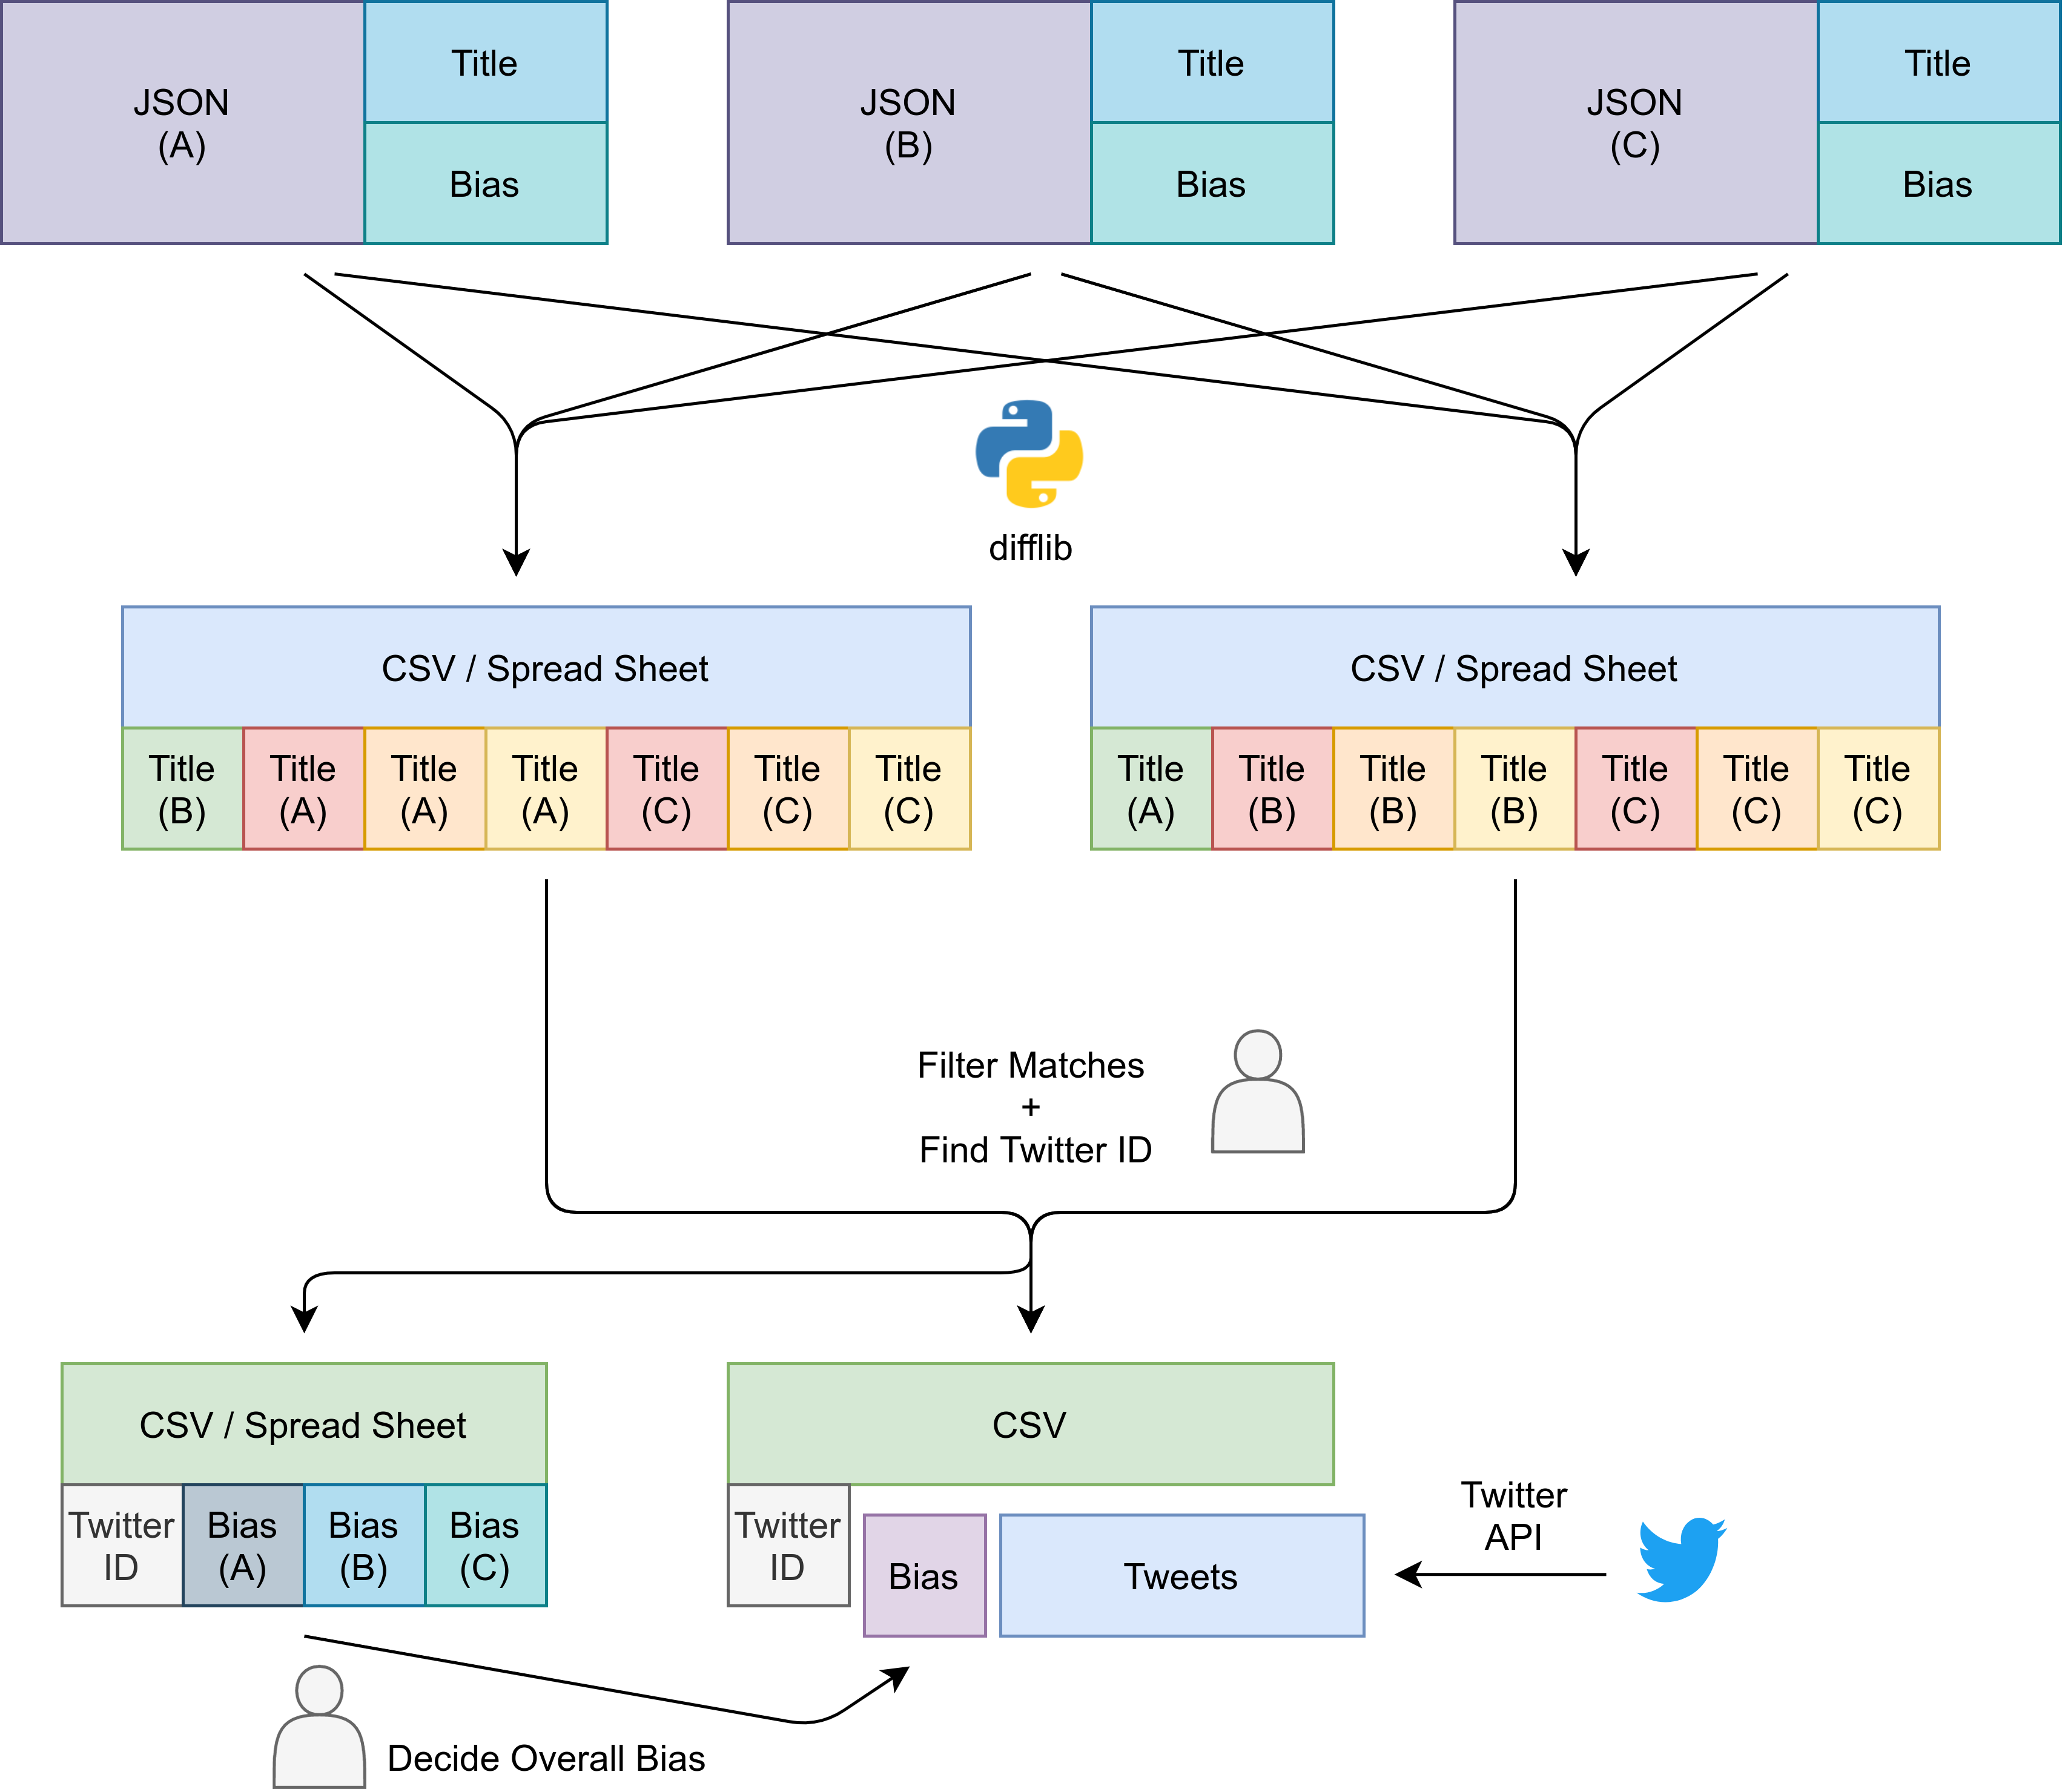
\includegraphics[width=0.7\textwidth]{figs/nlp_phase_1_summary.png}
  \caption{Summary of labeling process}
\end{figure}

\paragraph{How I labeled news channels}
To finalize the first step, I had to decide how to aggregate bias labels. Towards this end, I generated another table with columns including labeling data from all three sources for each matched channel title and exported it into a spreadsheet again. Row by row, I reviewed each label and if needed investigated more to come up with an accurate label as much as possible. In this process I tried to follow the following rules although in rare cases some rules may have been violated:
\begin{itemize}
  \item If at least two sources have the same point of view then their common view should be chosen.
  \item If there are only two sources, and they have opinions with difference of 1 then the bias label nearer to the center left or to the center right should be chosen.
  \item Otherwise, internet search and further investigation is needed.
  \item For the floating point labeling use -9 and 9 as boundaries between Left (Right) and Center-Left (Center-Right).
\end{itemize}
I labeled each news channel with an integer number from -2 to 2 which is equivalent to "Left", "Center-Left", "Center", "Center-Right", and "Right" respectively.

\paragraph{How I collected tweets}
I used official Twitter API via two standard developer accounts in parallel on a virtual private server. With ridiculously low rate limits, the process of collecting tweets from 458 accounts\footnote{Seven news channels did not have a Twitter account.} took about 12 hours. Using this method, 1,179,794 tweets have been collected. It has to be mentioned that Twitter allows up to only 3K latest tweets to be collected from each account via an standard developer account.

\section{Data Preprocessing}

\subsection{Sentence and Word Braking}
I used NLTK library for breaking tweets into sentences and words. Each tweet, has been broken into two or three sentences on average due to the short length of the original unit of data. Furthermore, word braking has been done in two steps. First, using NLTK word tokenizer a list of tokens has been generated from each tweet and saved. Second, filtered out non-alpha tokens using python str.isalpha function to generate a word list from each token list.
In this phase, stop-words has been removed from tokens and words but for the next phases this hardcoded approach will be replaced with a more dynamic approach of having an incrementally growing stop-word list and using it at runtime.

\subsection{Data Cleaning}
I used tweet-preprocessor python library to clean tweets. With the help of this library, I removed URLs, Mentions, Reserved Words (RT, FAV), Emojis, Smileys, and Numbers. I did not remove Hashtags because many are used instead of normal words in the sentences, hence containing essential semantics. This step needed more time and effort to be considered completed because the results of analyses show that some unwanted words seem important. Most of them are channel titles and unnormalized hashtags which are repeated over and over by few channels. To mitigate this issue, I removed the words and tokens that are only used by less than 4 channels.

\section{Data Statistics}
I used the following libraries in this step:
\begin{itemize}
  \item tabulate: to generate grid and latex formatted tables
  \item matplotlib: to generate graphs
  \item seaborn: to generate graphs
  \item tqdm: to show progress bar in the cli
\end{itemize}

\pagebreak

\subsection{Tweets Count}
\begin{center}
\CatchFileDef{\CountTweetsTable}{figs/count_tweets/table.latex.txt}
  
\CountTweetsTable
\begin{figure}[h!]
  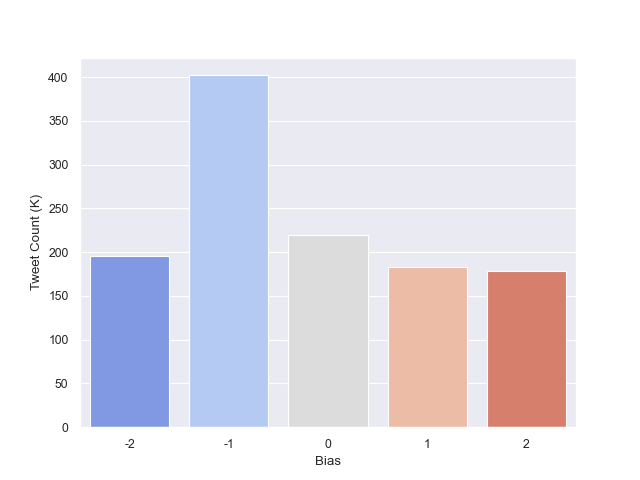
\includegraphics[width=0.55\textwidth]{figs/count_tweets/count_tweets.png}
\end{figure}
\end{center}

% \begin{figure}[h!]
%   \begin{floatrow}
%   \ffigbox{%
%   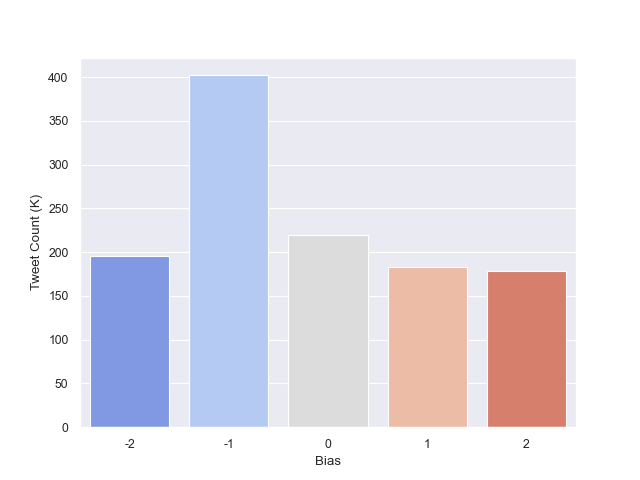
\includegraphics[width=0.5\textwidth]{figs/count_tweets/count_tweets.png}%
%   }{%
%     \caption{A figure}%
%   }
%   \capbtabbox{%
%   \begin{tabular}{rr}
%         \hline
%             Bias &   Tweet Count \\
%         \hline
%             -2 &        196214 \\
%             -1 &        404790 \\
%             0 &        220807 \\
%             1 &        184506 \\
%             2 &        177995 \\
%         \hline
%         \end{tabular}
%   }{%
%     \caption{A table}%
%   }
%   \end{floatrow}
%   \end{figure}

\subsection{Sentences Count}
\begin{center}

\CatchFileDef{\CountSentencesTable}{figs/count_sentences/table.latex.txt}

\CountSentencesTable
\begin{figure}[h!]
  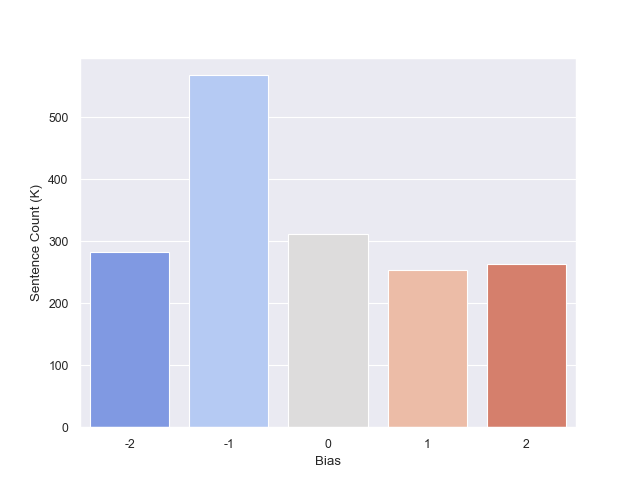
\includegraphics[width=0.55\textwidth]{figs/count_sentences/count_sentences.png}
\end{figure}
\end{center}


\subsection{Tokens \& Words Count}
\begin{center}

\CatchFileDef{\CountTWTable}{figs/count_words/table.latex.txt}

\CountTWTable
\begin{figure}[h!]
  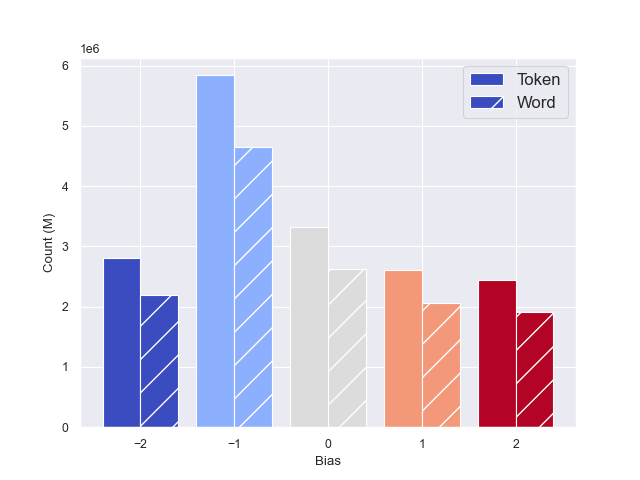
\includegraphics[width=0.55\textwidth]{figs/count_words/count_tokens_words.png}
\end{figure}
\end{center}


\subsection{Unique Words Count}
\begin{center}

\CatchFileDef{\CountUWTable}{figs/count_unique_words/table.latex.txt}

\CountUWTable
\begin{figure}[h!]
  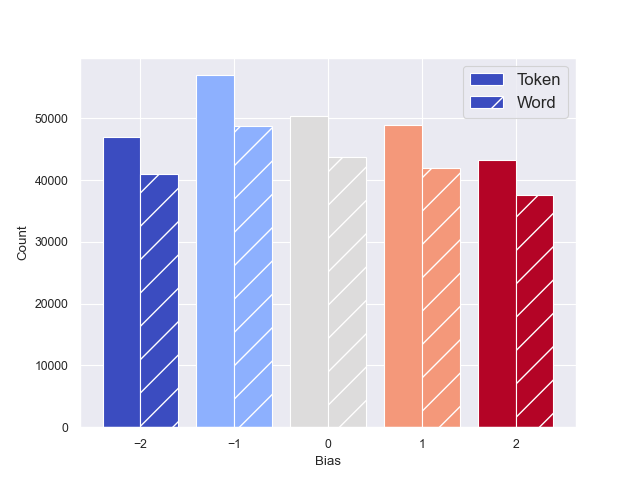
\includegraphics[width=0.55\textwidth]{figs/count_unique_words/count_tokens_words.png}
\end{figure}
\end{center}


\subsection{Common Tokens Count}
\begin{center}

\CatchFileDef{\CountCTTable}{figs/count_cuc_words/table_c_t.latex.txt}

\CountCTTable
\begin{figure}[h!]
  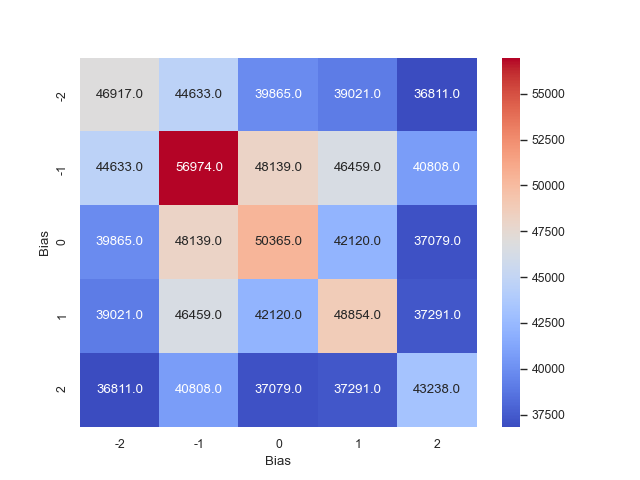
\includegraphics[width=0.55\textwidth]{figs/count_cuc_words/c_t.png}
\end{figure}
\end{center}

\subsection{Uncommon Tokens Count}
\begin{center}

\CatchFileDef{\CountUCTTable}{figs/count_cuc_words/table_uc_t.latex.txt}

\CountUCTTable
\begin{figure}[h!]
  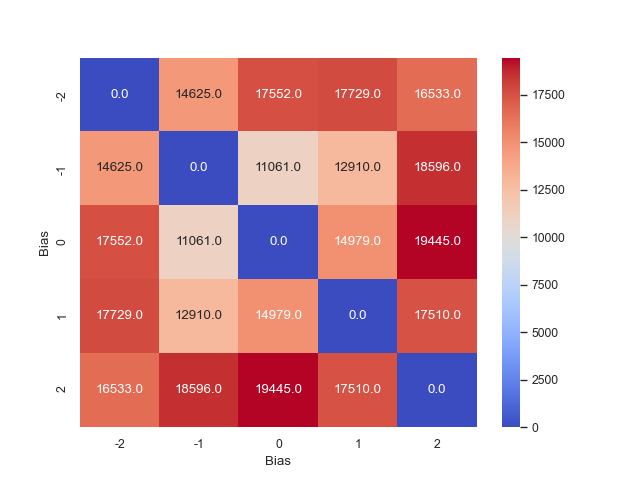
\includegraphics[width=0.55\textwidth]{figs/count_cuc_words/uc_t.png}
\end{figure}
\end{center}


\subsection{Common Words Count}
\begin{center}

\CatchFileDef{\CountCWTable}{figs/count_cuc_words/table_c_w.latex.txt}

\CountCWTable
\begin{figure}[h!]
  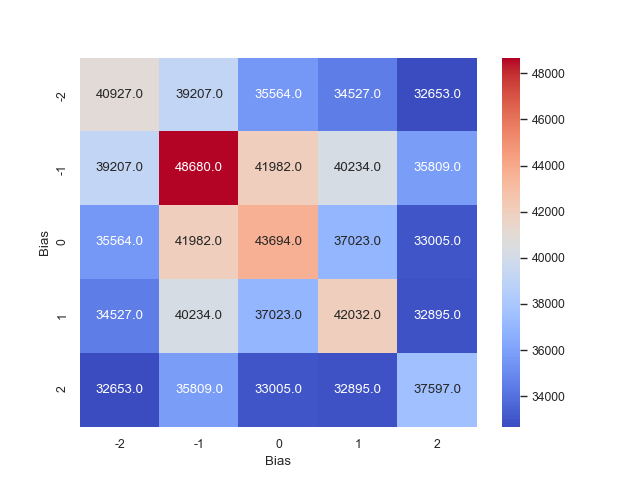
\includegraphics[width=0.55\textwidth]{figs/count_cuc_words/c_w.png}
\end{figure}
\end{center}


\subsection{Uncommon Words Count}
\begin{center}

\CatchFileDef{\CountUCWTable}{figs/count_cuc_words/table_uc_w.latex.txt}

\CountUCWTable
\begin{figure}[h!]
  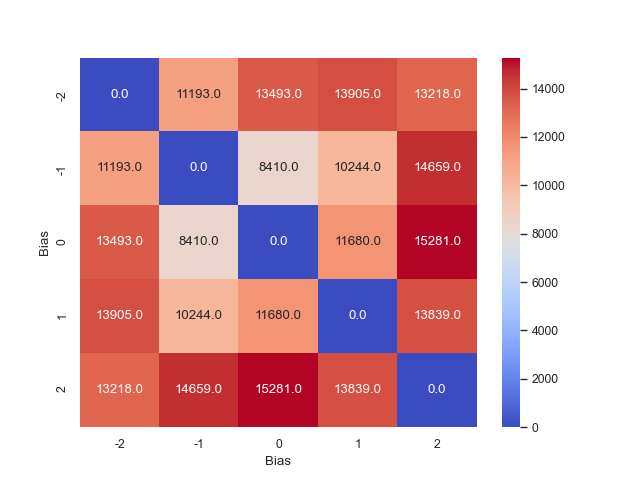
\includegraphics[width=0.55\textwidth]{figs/count_cuc_words/uc_w.png}
\end{figure}
\end{center}


\subsection{Top Ten Uncommon Tokens}
\begin{center}

\CatchFileDef{\TTUCTTable}{figs/top_ten_uc_words/table_token.latex.txt}

\resizebox{\columnwidth}{!}
{
\TTUCTTable
}
\begin{figure}[h!]
  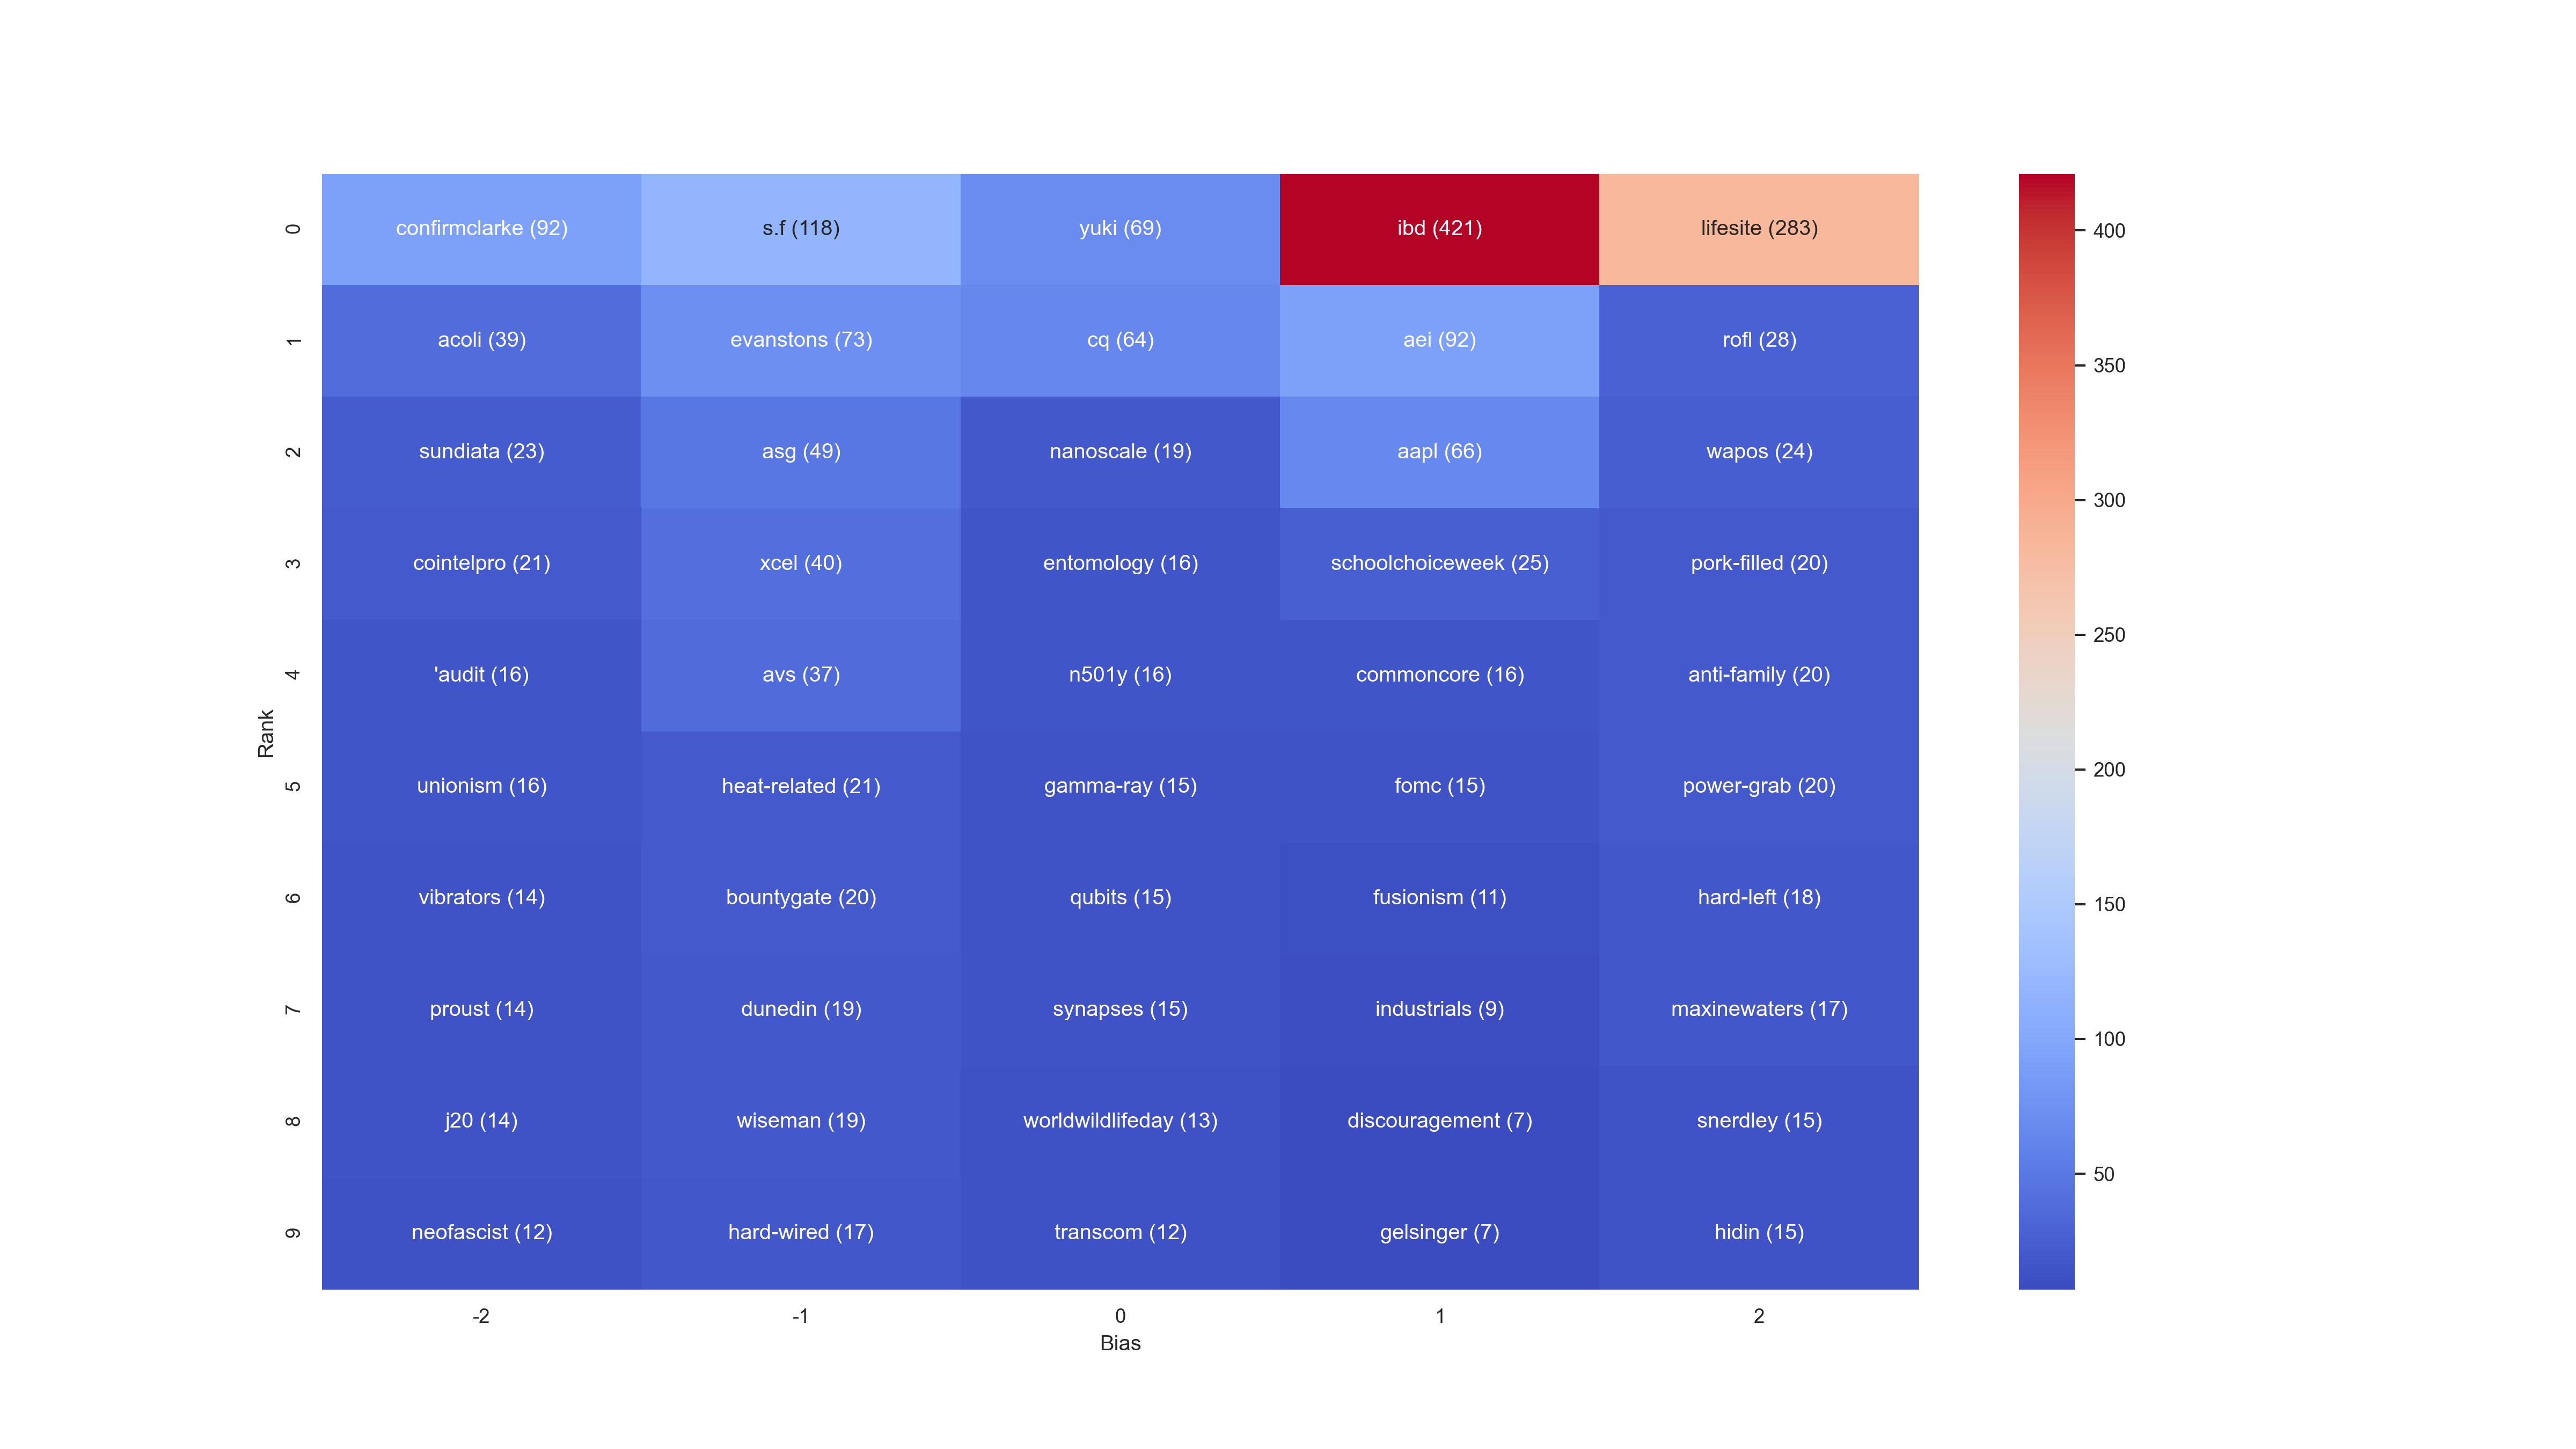
\includegraphics[width=1.1\textwidth]{figs/top_ten_uc_words/token.png}
\end{figure}
\end{center}

\pagebreak

\subsection{Top Ten Uncommon Words}
\begin{center}

\CatchFileDef{\TTUCTable}{figs/top_ten_uc_words/table_word.latex.txt}

\resizebox{\columnwidth}{!}
{
\TTUCTable
}
\begin{figure}[h!]
  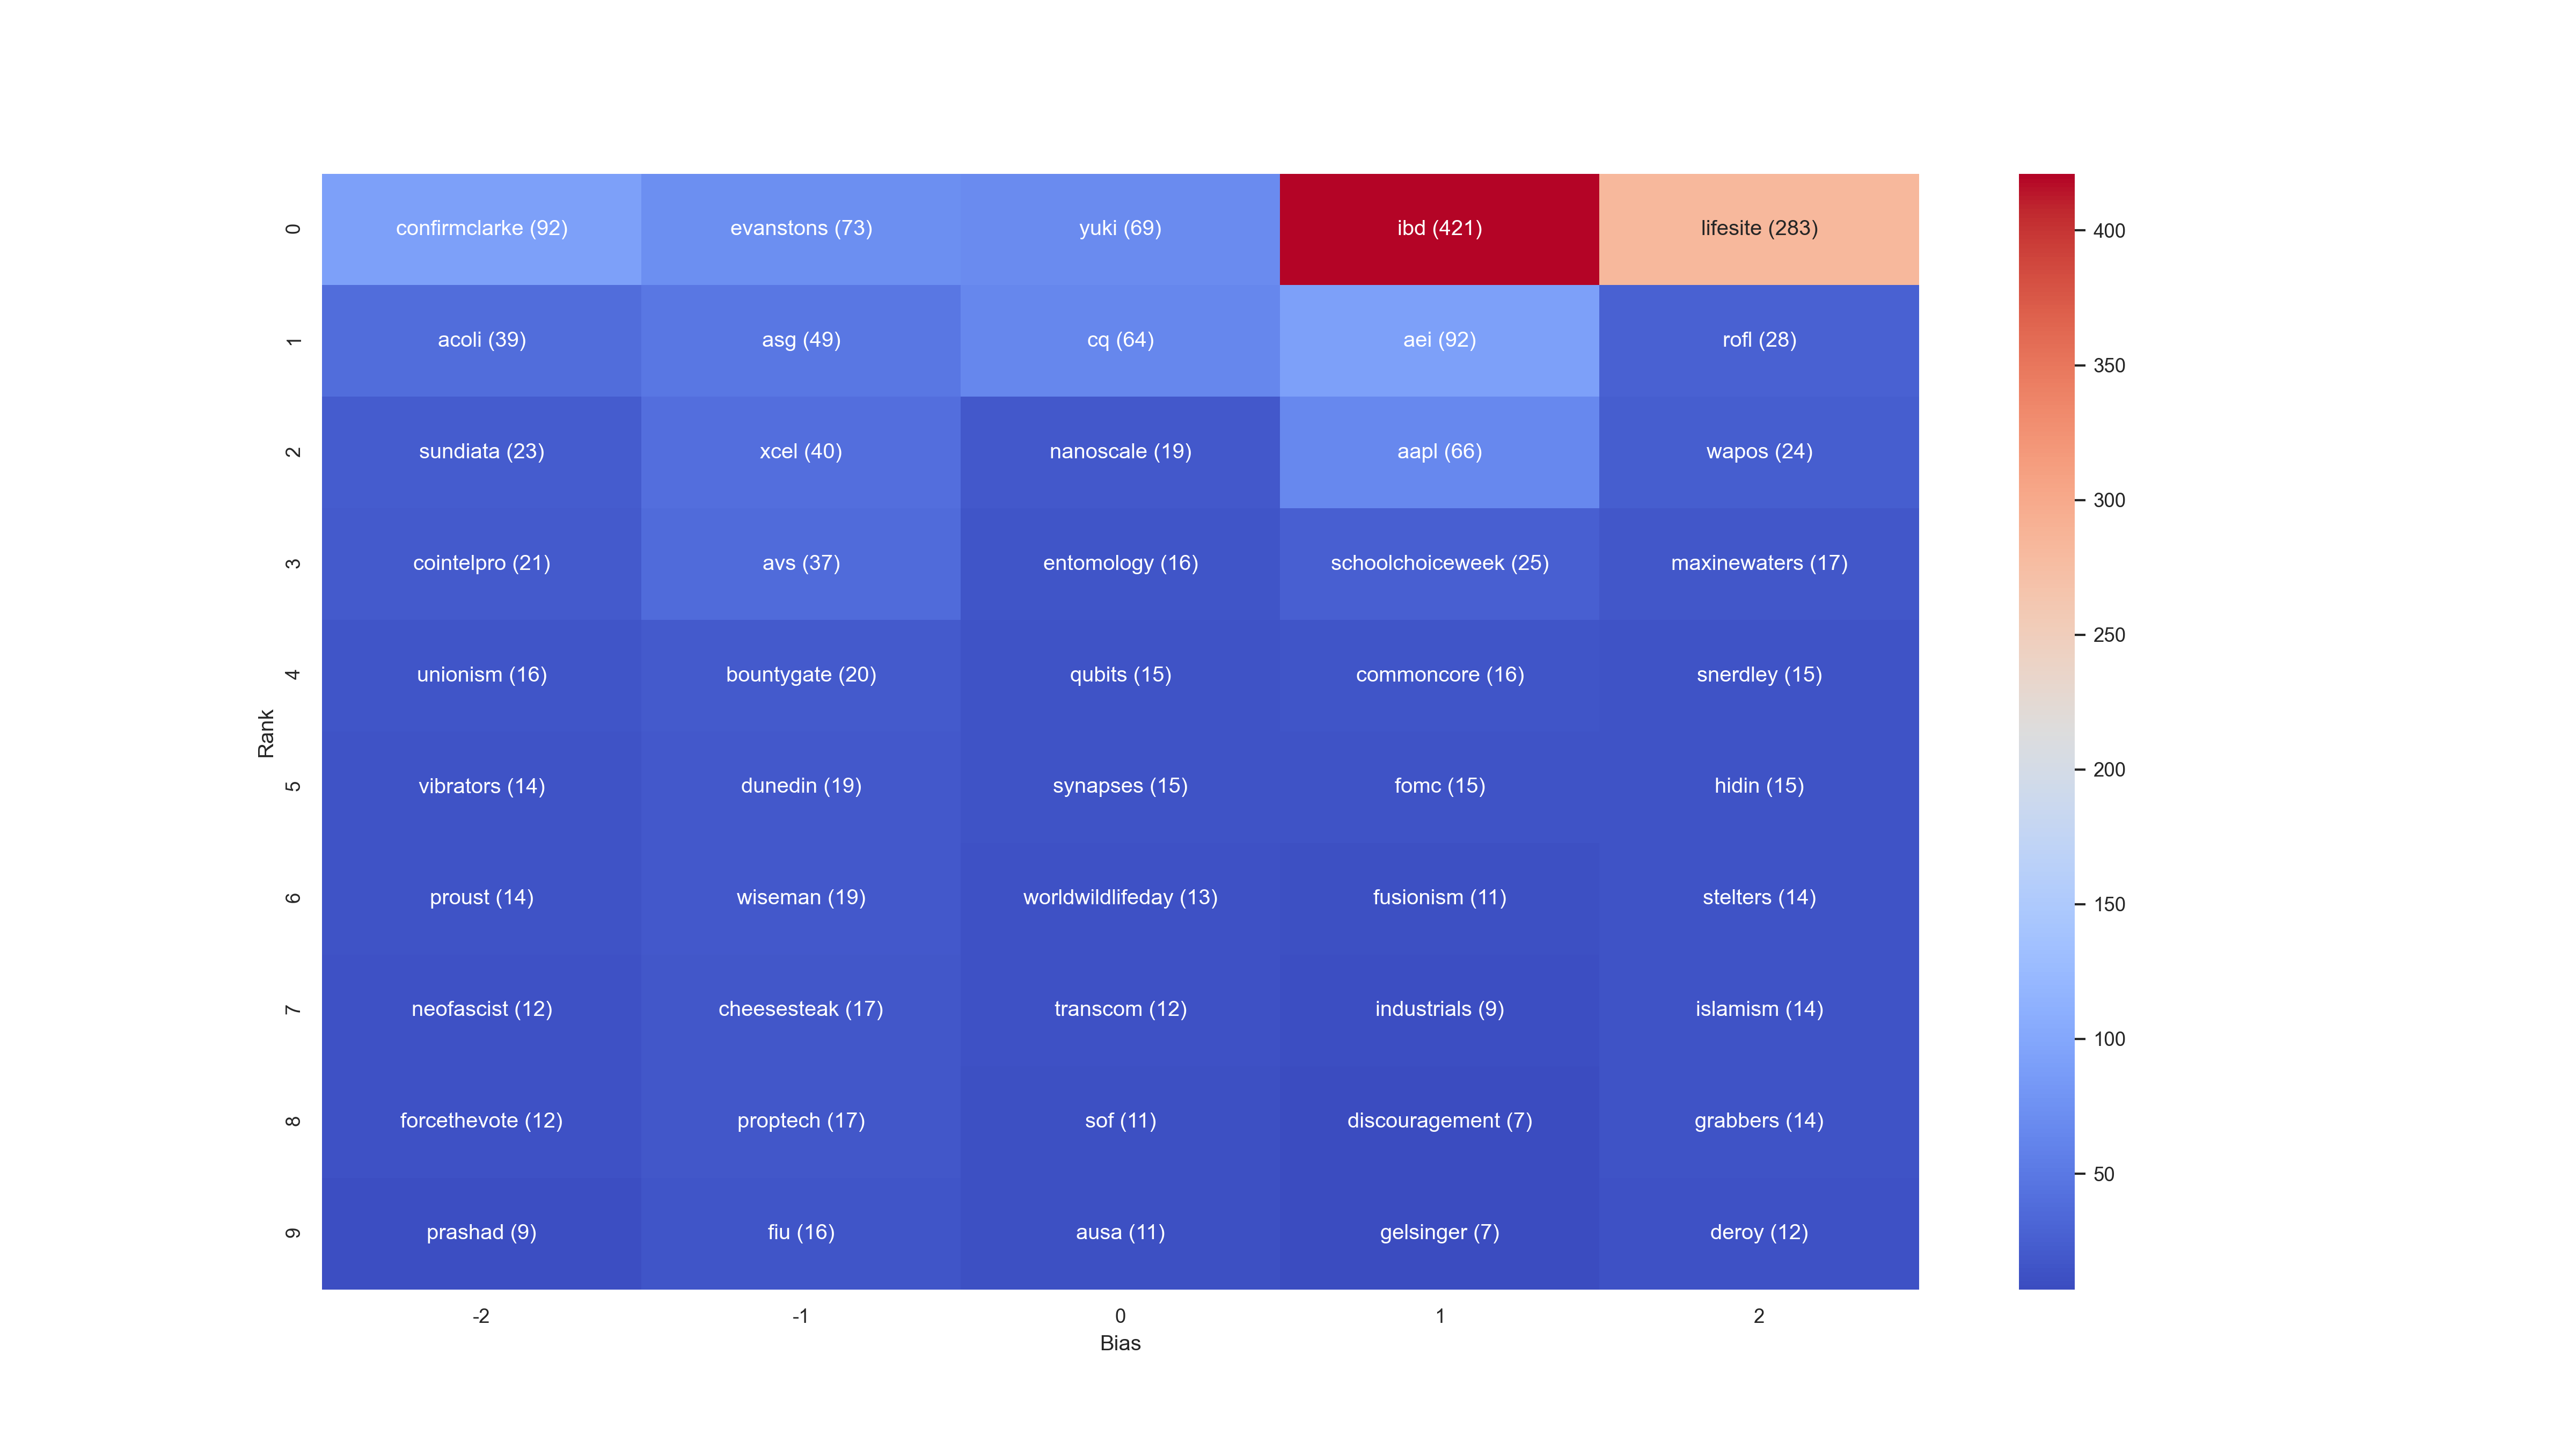
\includegraphics[width=1.1\textwidth]{figs/top_ten_uc_words/word.png}
\end{figure}
\end{center}

\pagebreak

\subsection{Top Ten Common Tokens Based on Relative Normalized Frequency}
\subsubsection{Rank 0}
\begin{center}

\CatchFileDef{\TTRNFTable}{figs/top_ten_rnf/table_rnf_t_rank_0.latex.txt}

\resizebox{\columnwidth}{!}
{
\TTRNFTable
}
\begin{figure}[h!]
  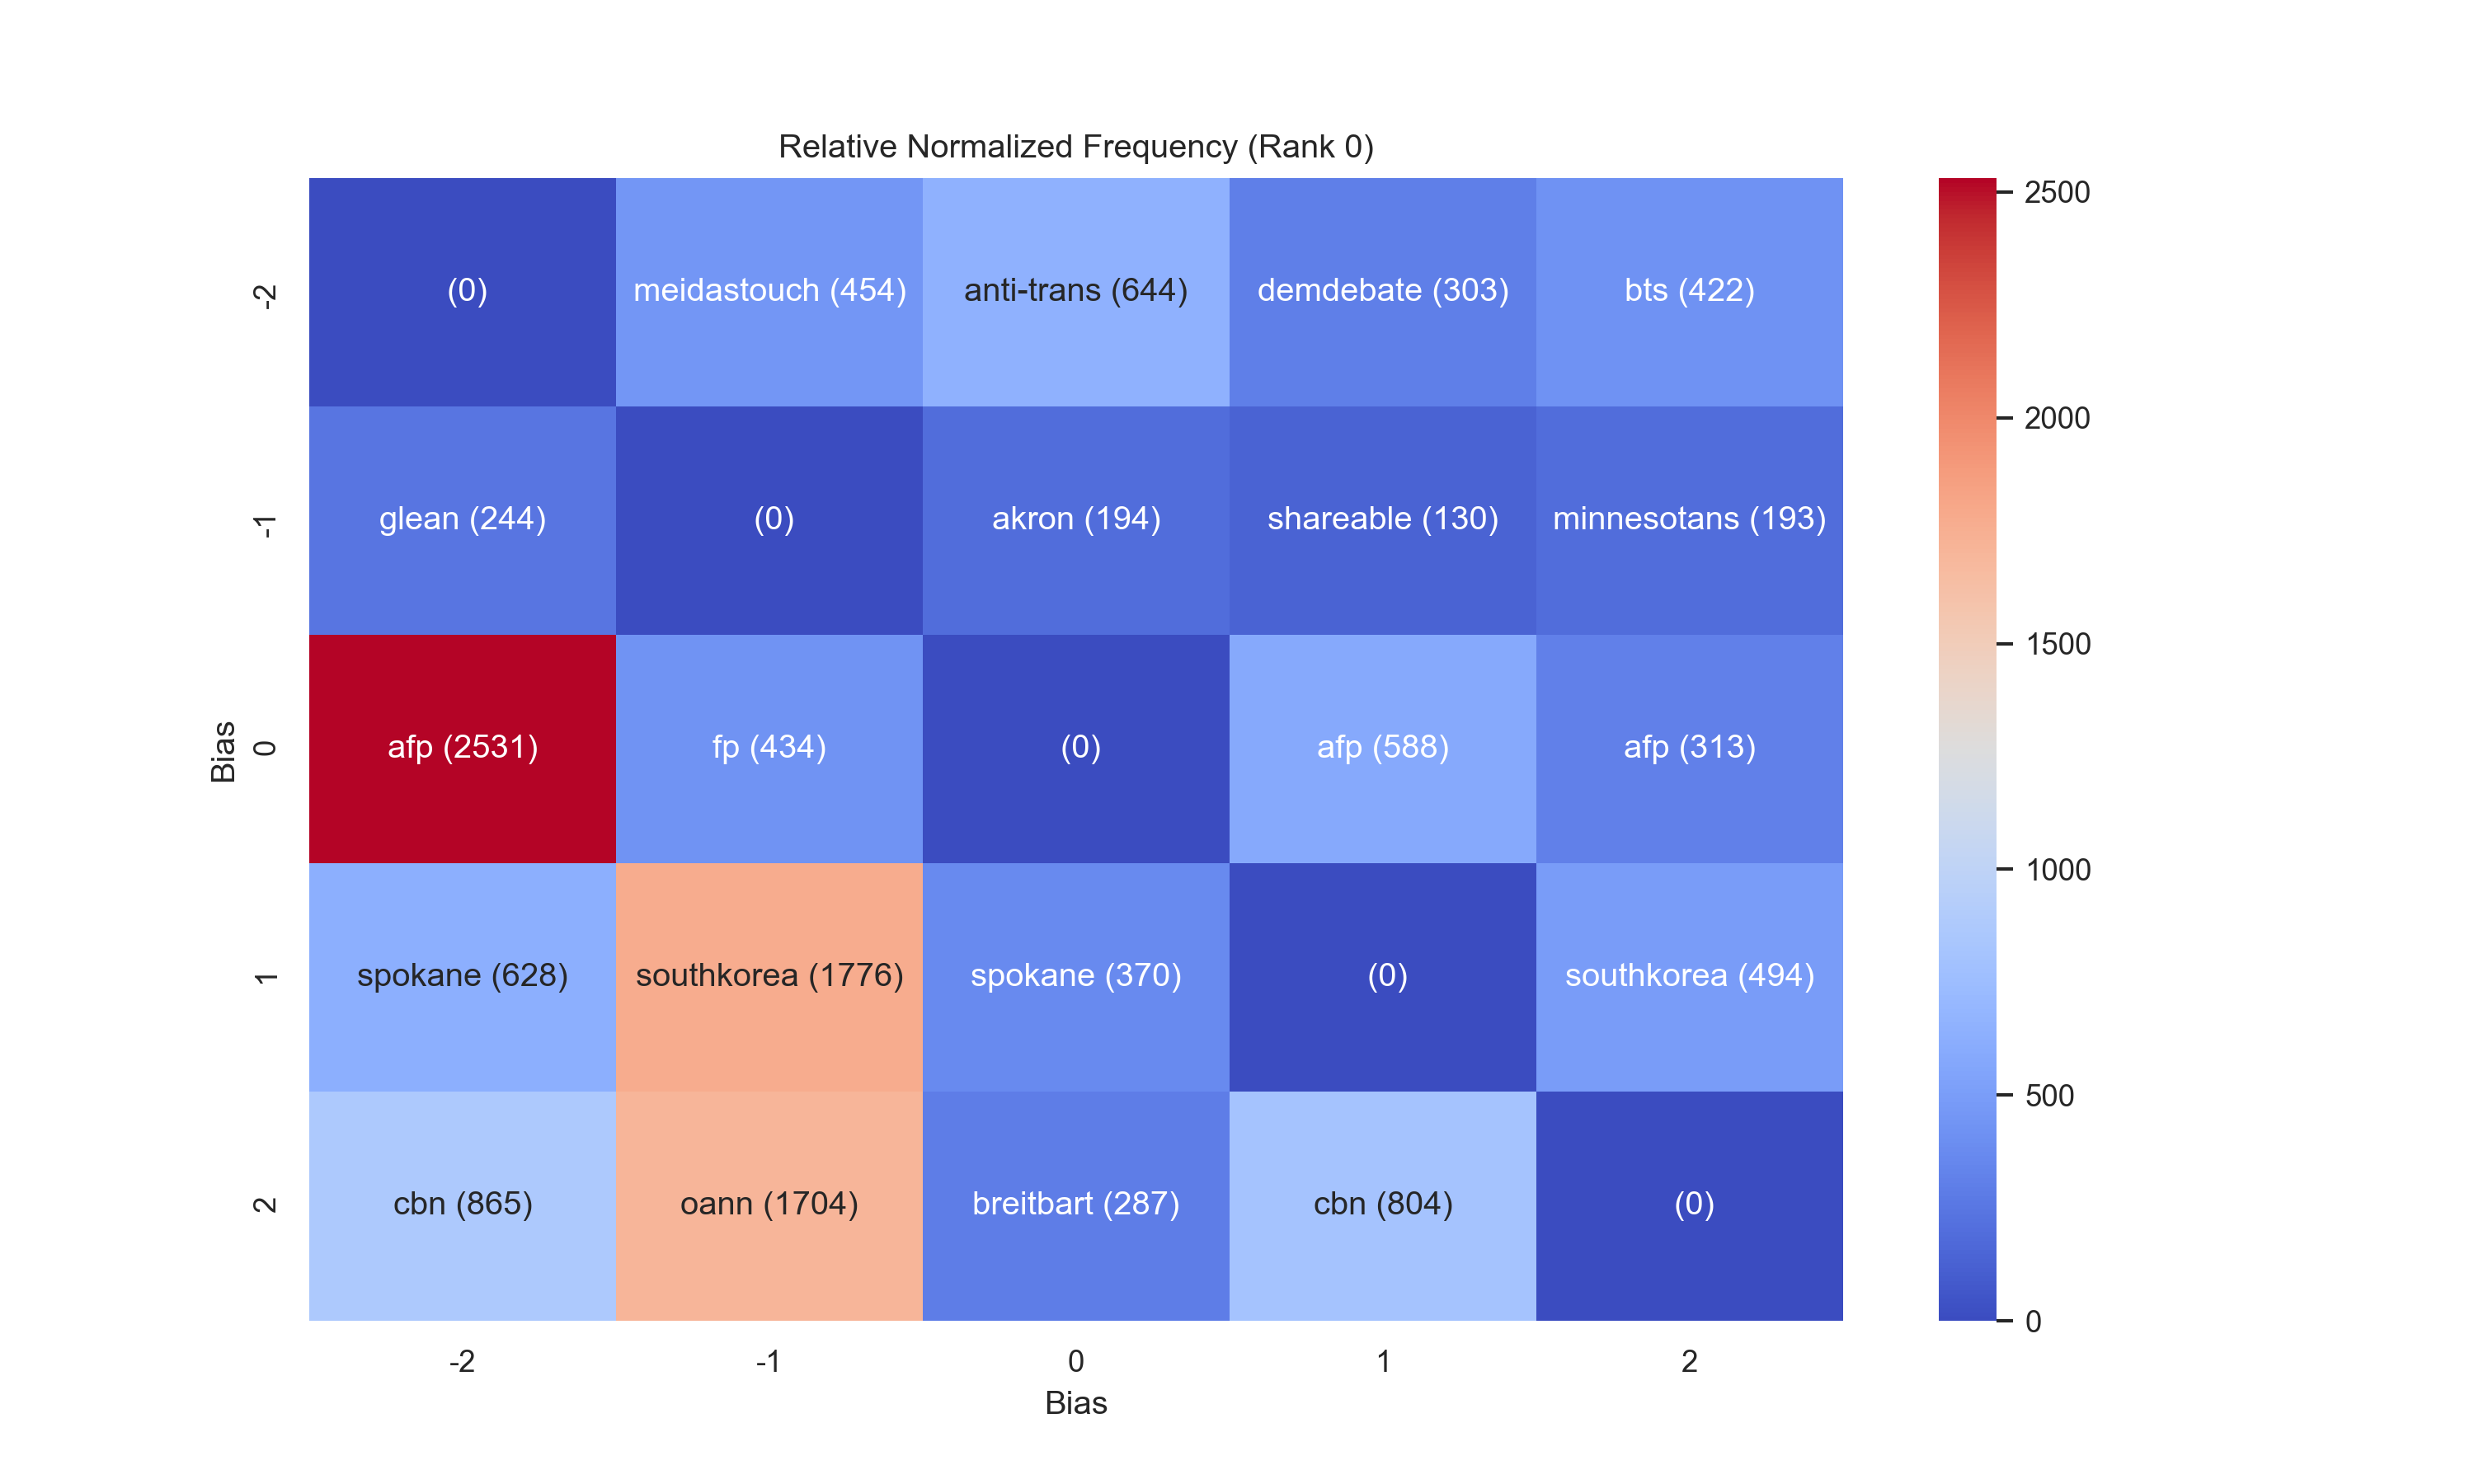
\includegraphics[width=0.6\textwidth]{figs/top_ten_rnf/rnf_t_rank_0.png}
\end{figure}
\end{center}

\subsubsection{Rank 1}
\begin{center}

\CatchFileDef{\TTRNFTable}{figs/top_ten_rnf/table_rnf_t_rank_1.latex.txt}

\resizebox{\columnwidth}{!}
{
\TTRNFTable
}
\begin{figure}[h!]
  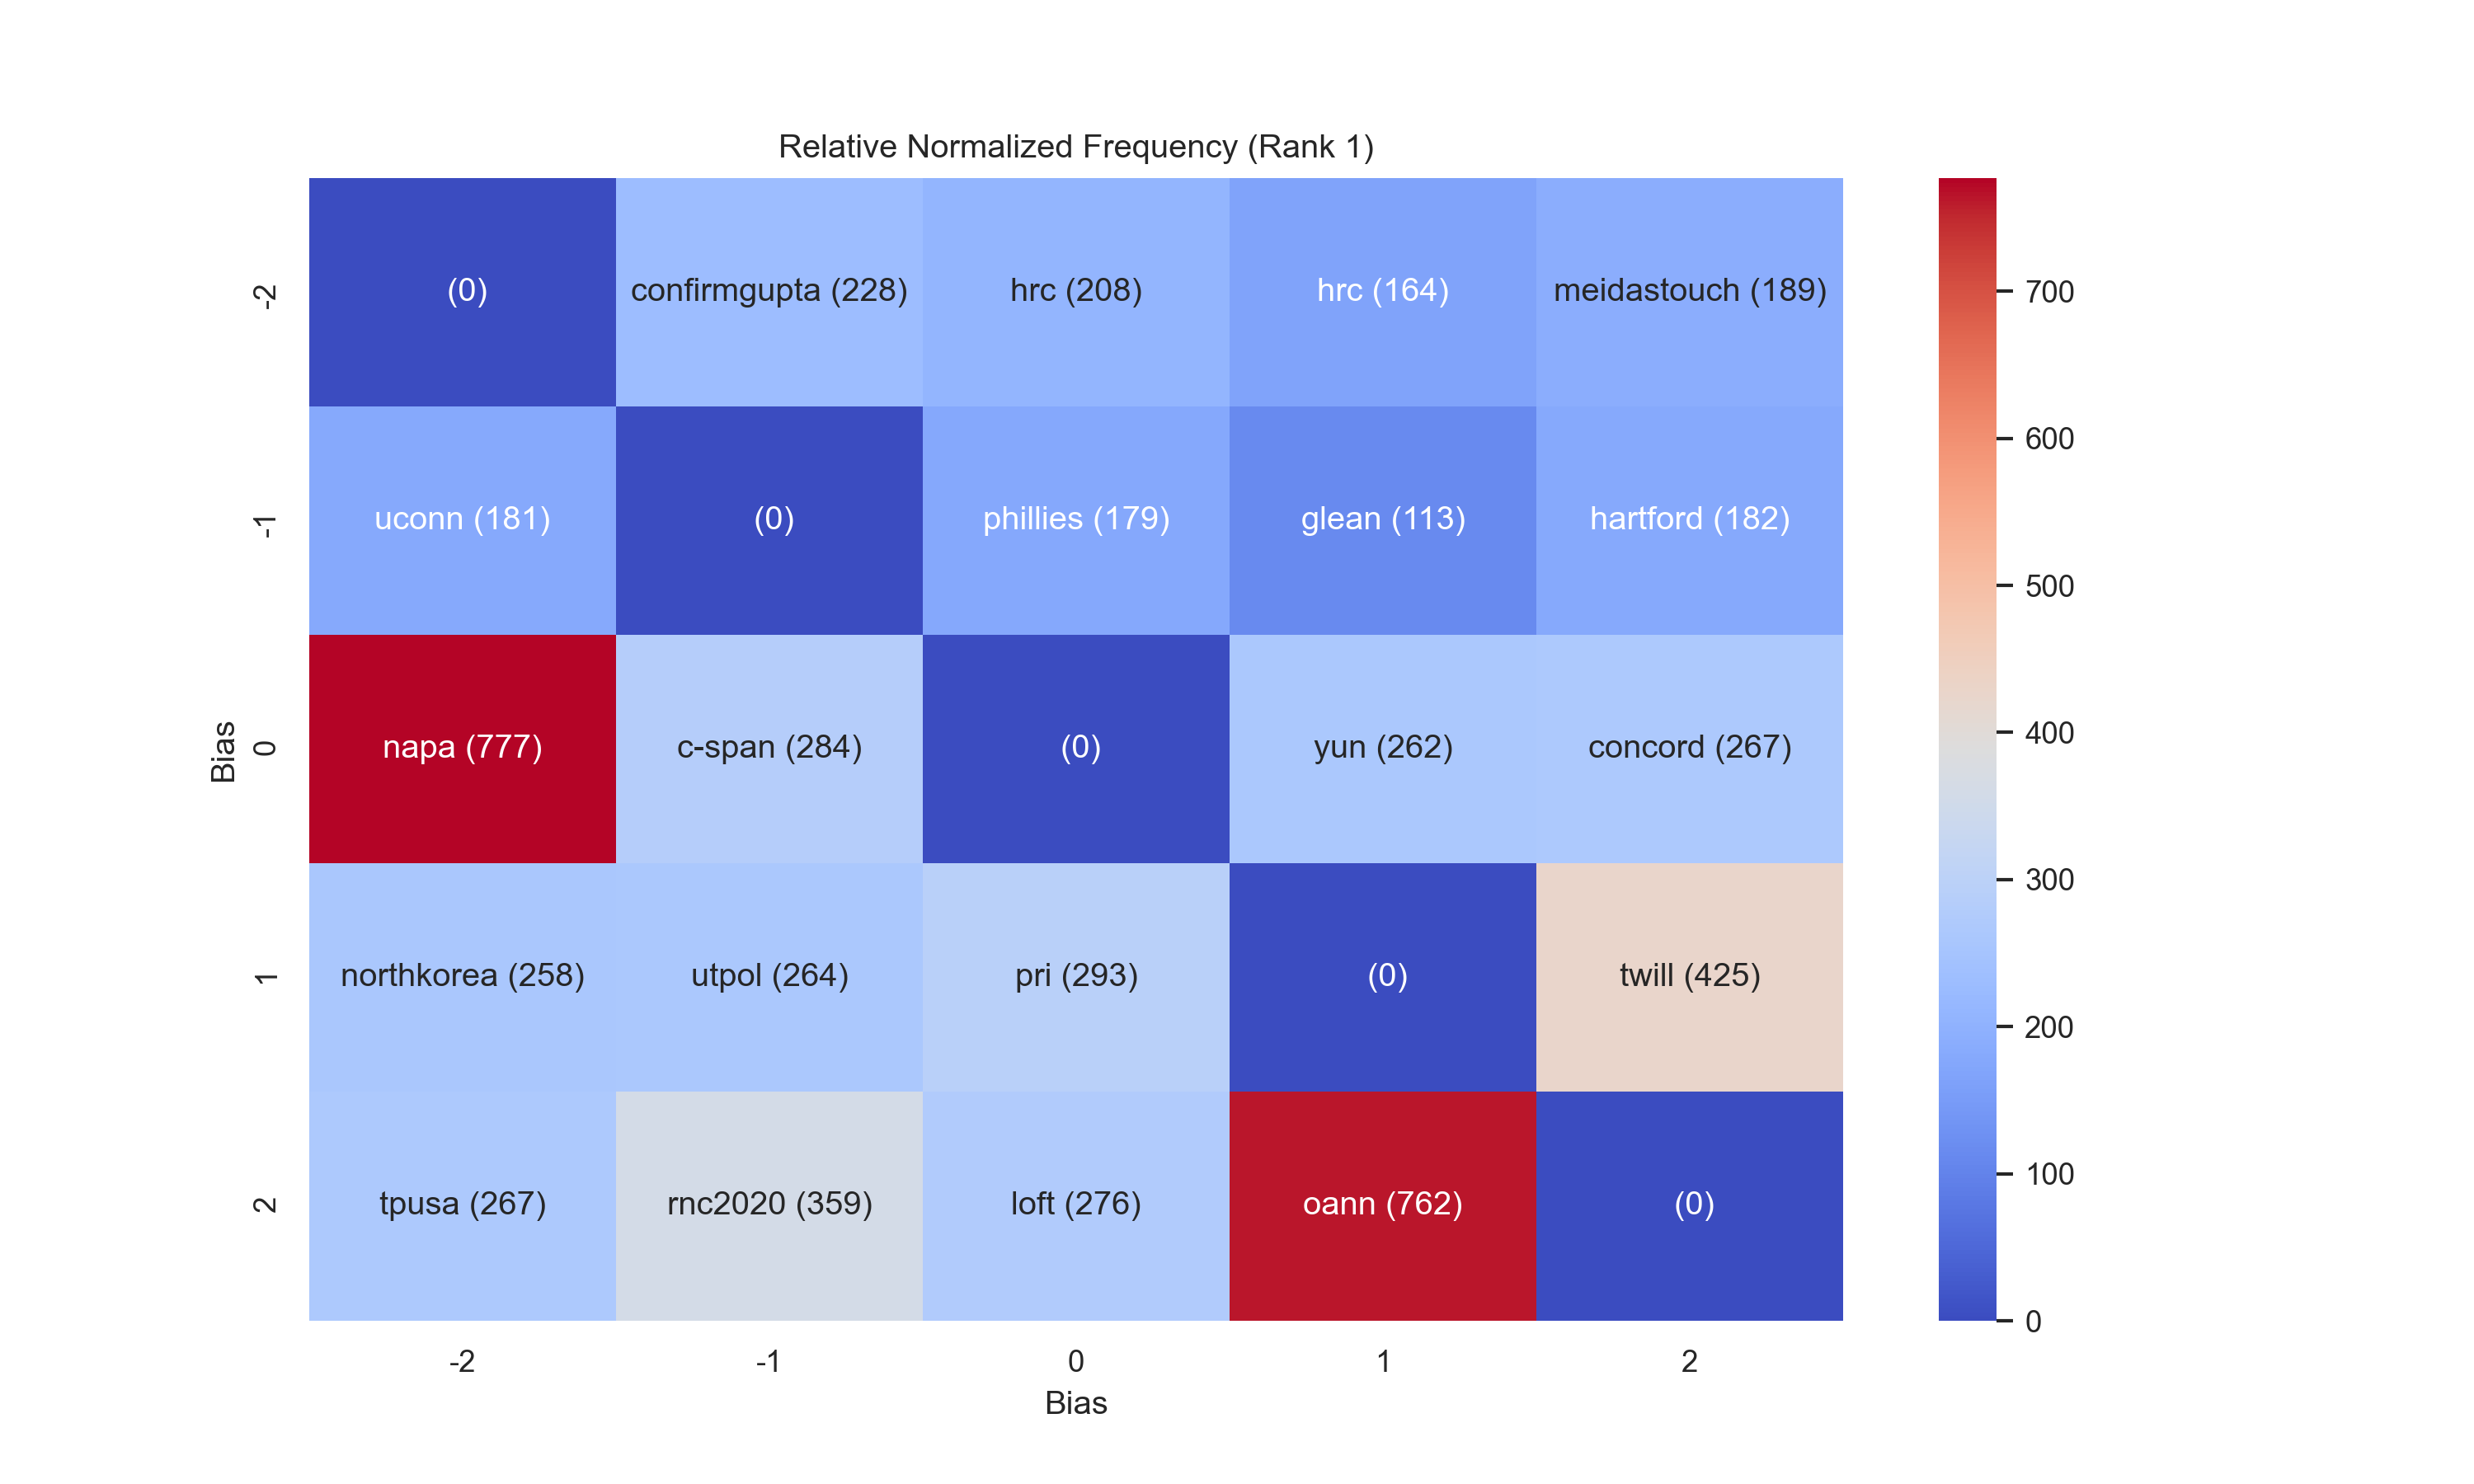
\includegraphics[width=0.6\textwidth]{figs/top_ten_rnf/rnf_t_rank_1.png}
\end{figure}
\end{center}

\pagebreak

\subsubsection{Rank 2}
\begin{center}

\CatchFileDef{\TTRNFTable}{figs/top_ten_rnf/table_rnf_t_rank_2.latex.txt}

\resizebox{\columnwidth}{!}
{
\TTRNFTable
}
\begin{figure}[h!]
  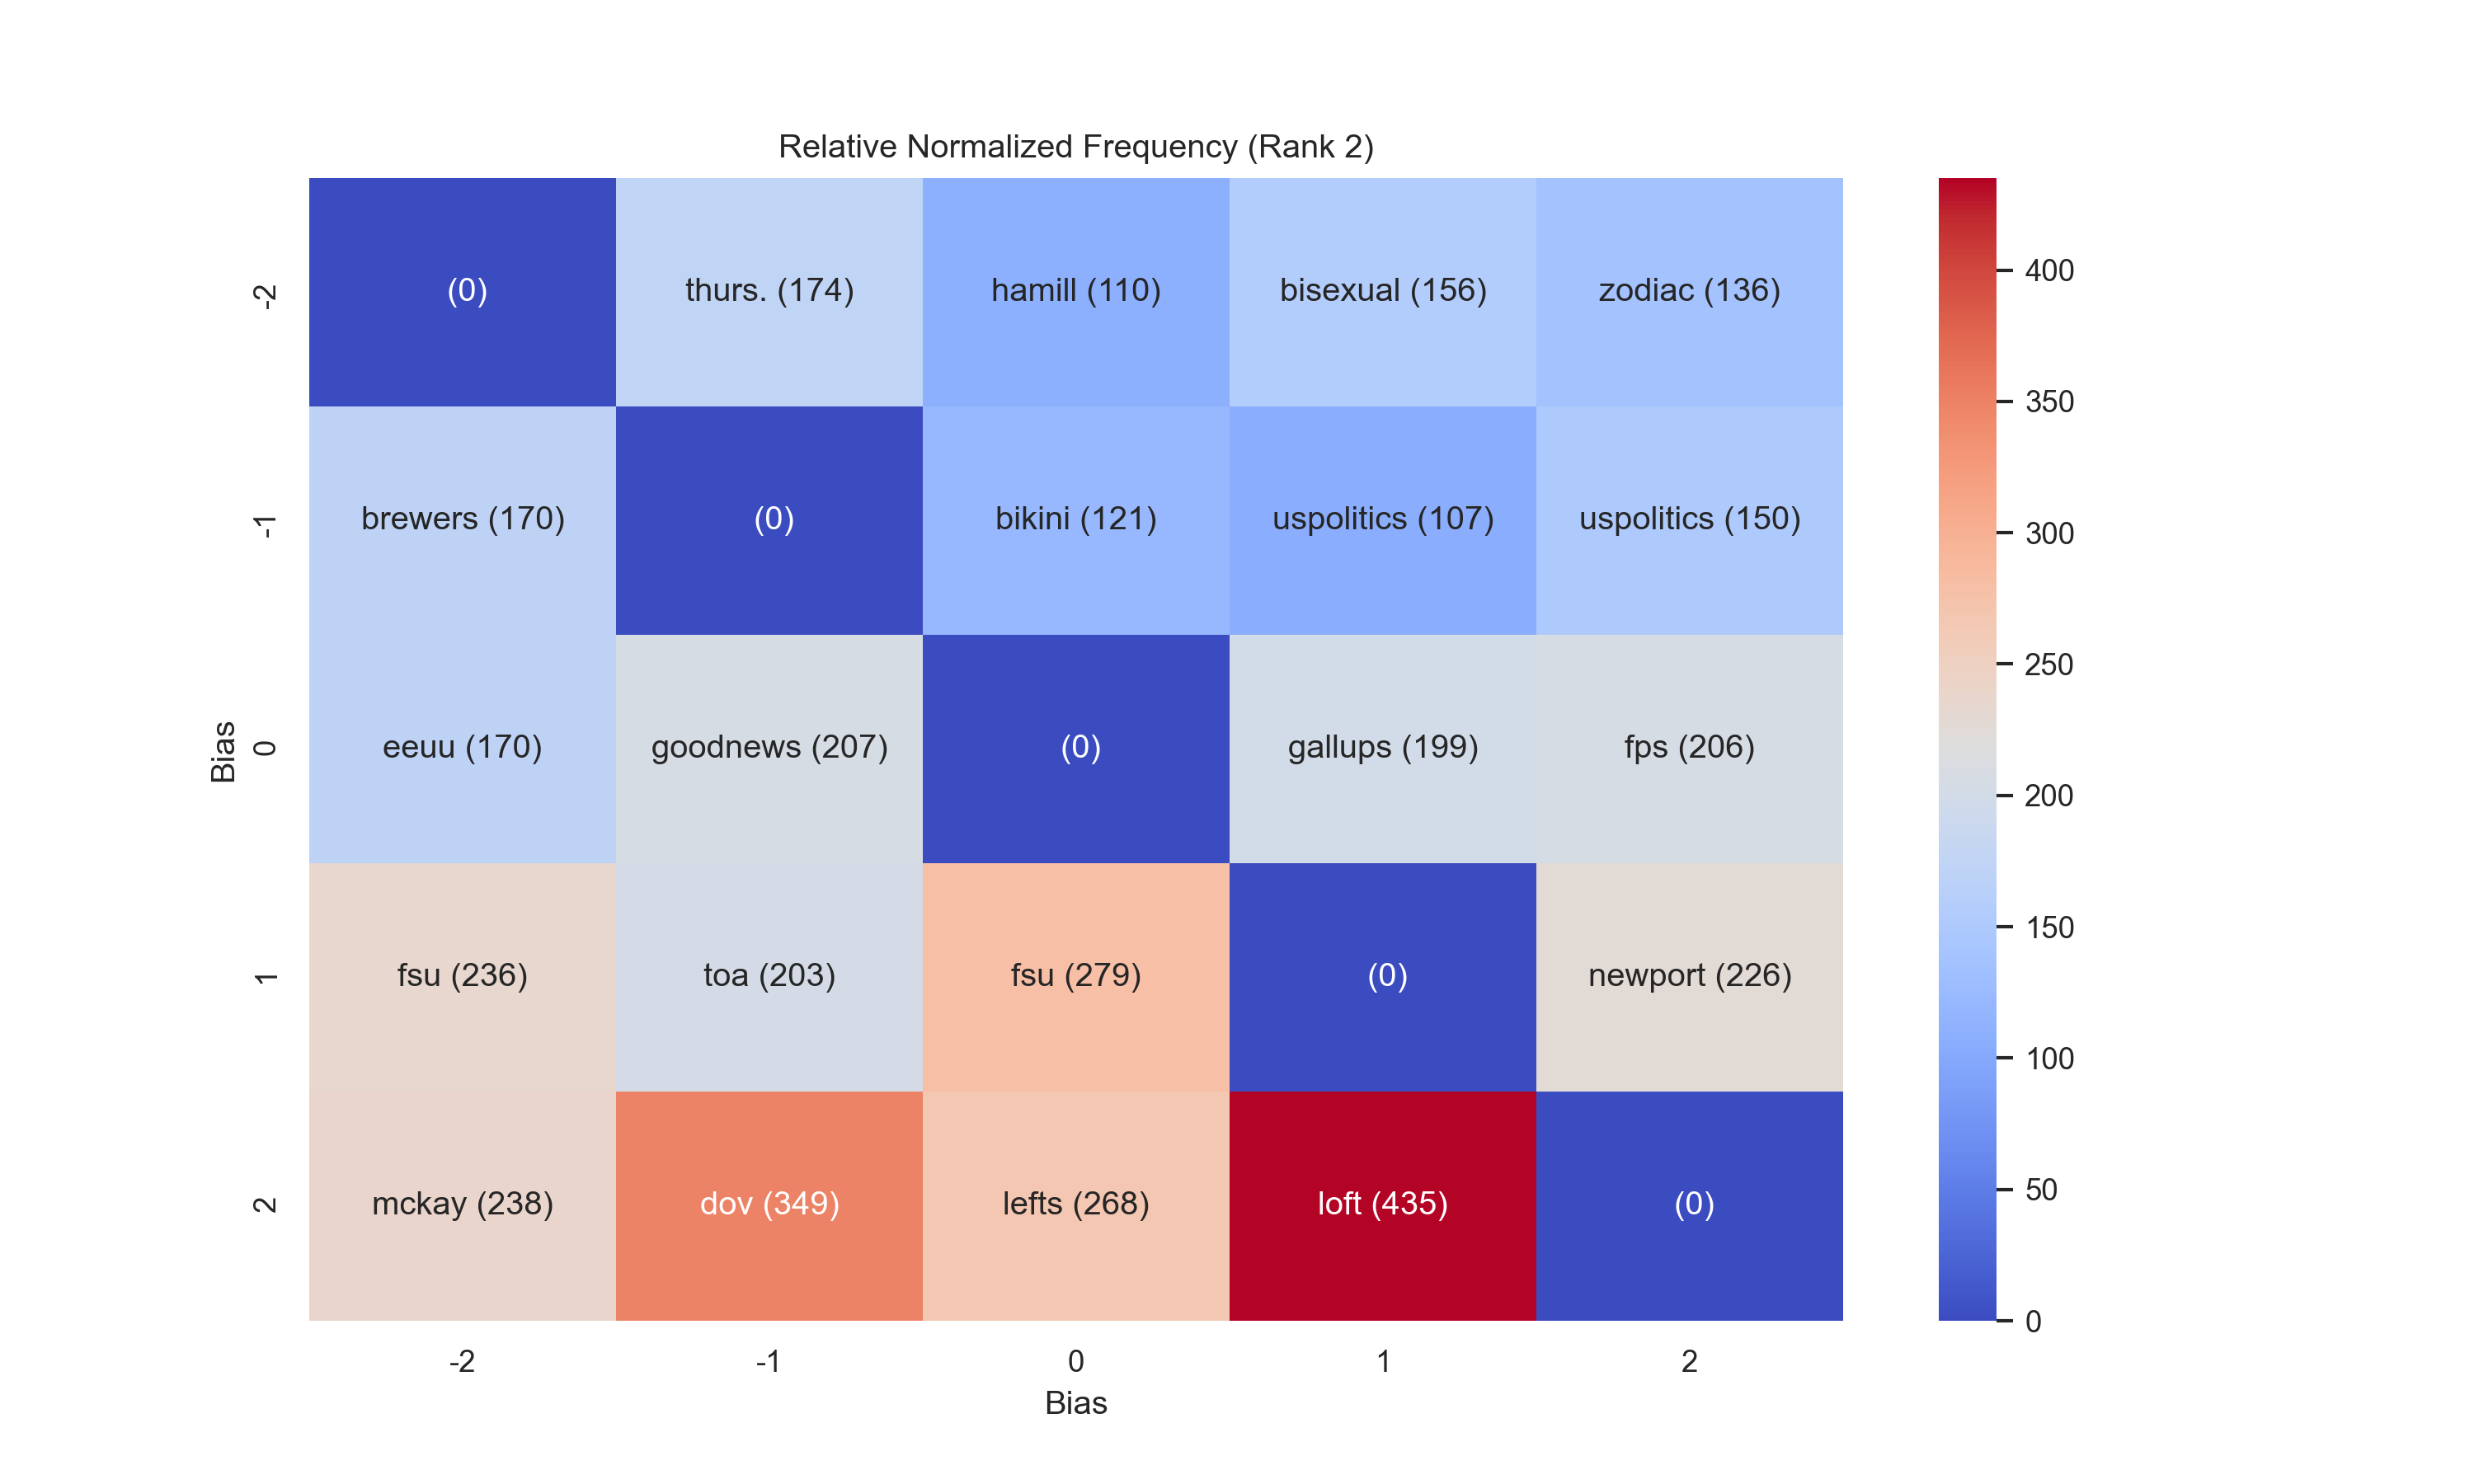
\includegraphics[width=0.6\textwidth]{figs/top_ten_rnf/rnf_t_rank_2.png}
\end{figure}
\end{center}

\subsubsection{Rank 3}
\begin{center}

\CatchFileDef{\TTRNFTable}{figs/top_ten_rnf/table_rnf_t_rank_3.latex.txt}

\resizebox{\columnwidth}{!}
{
\TTRNFTable
}
\begin{figure}[h!]
  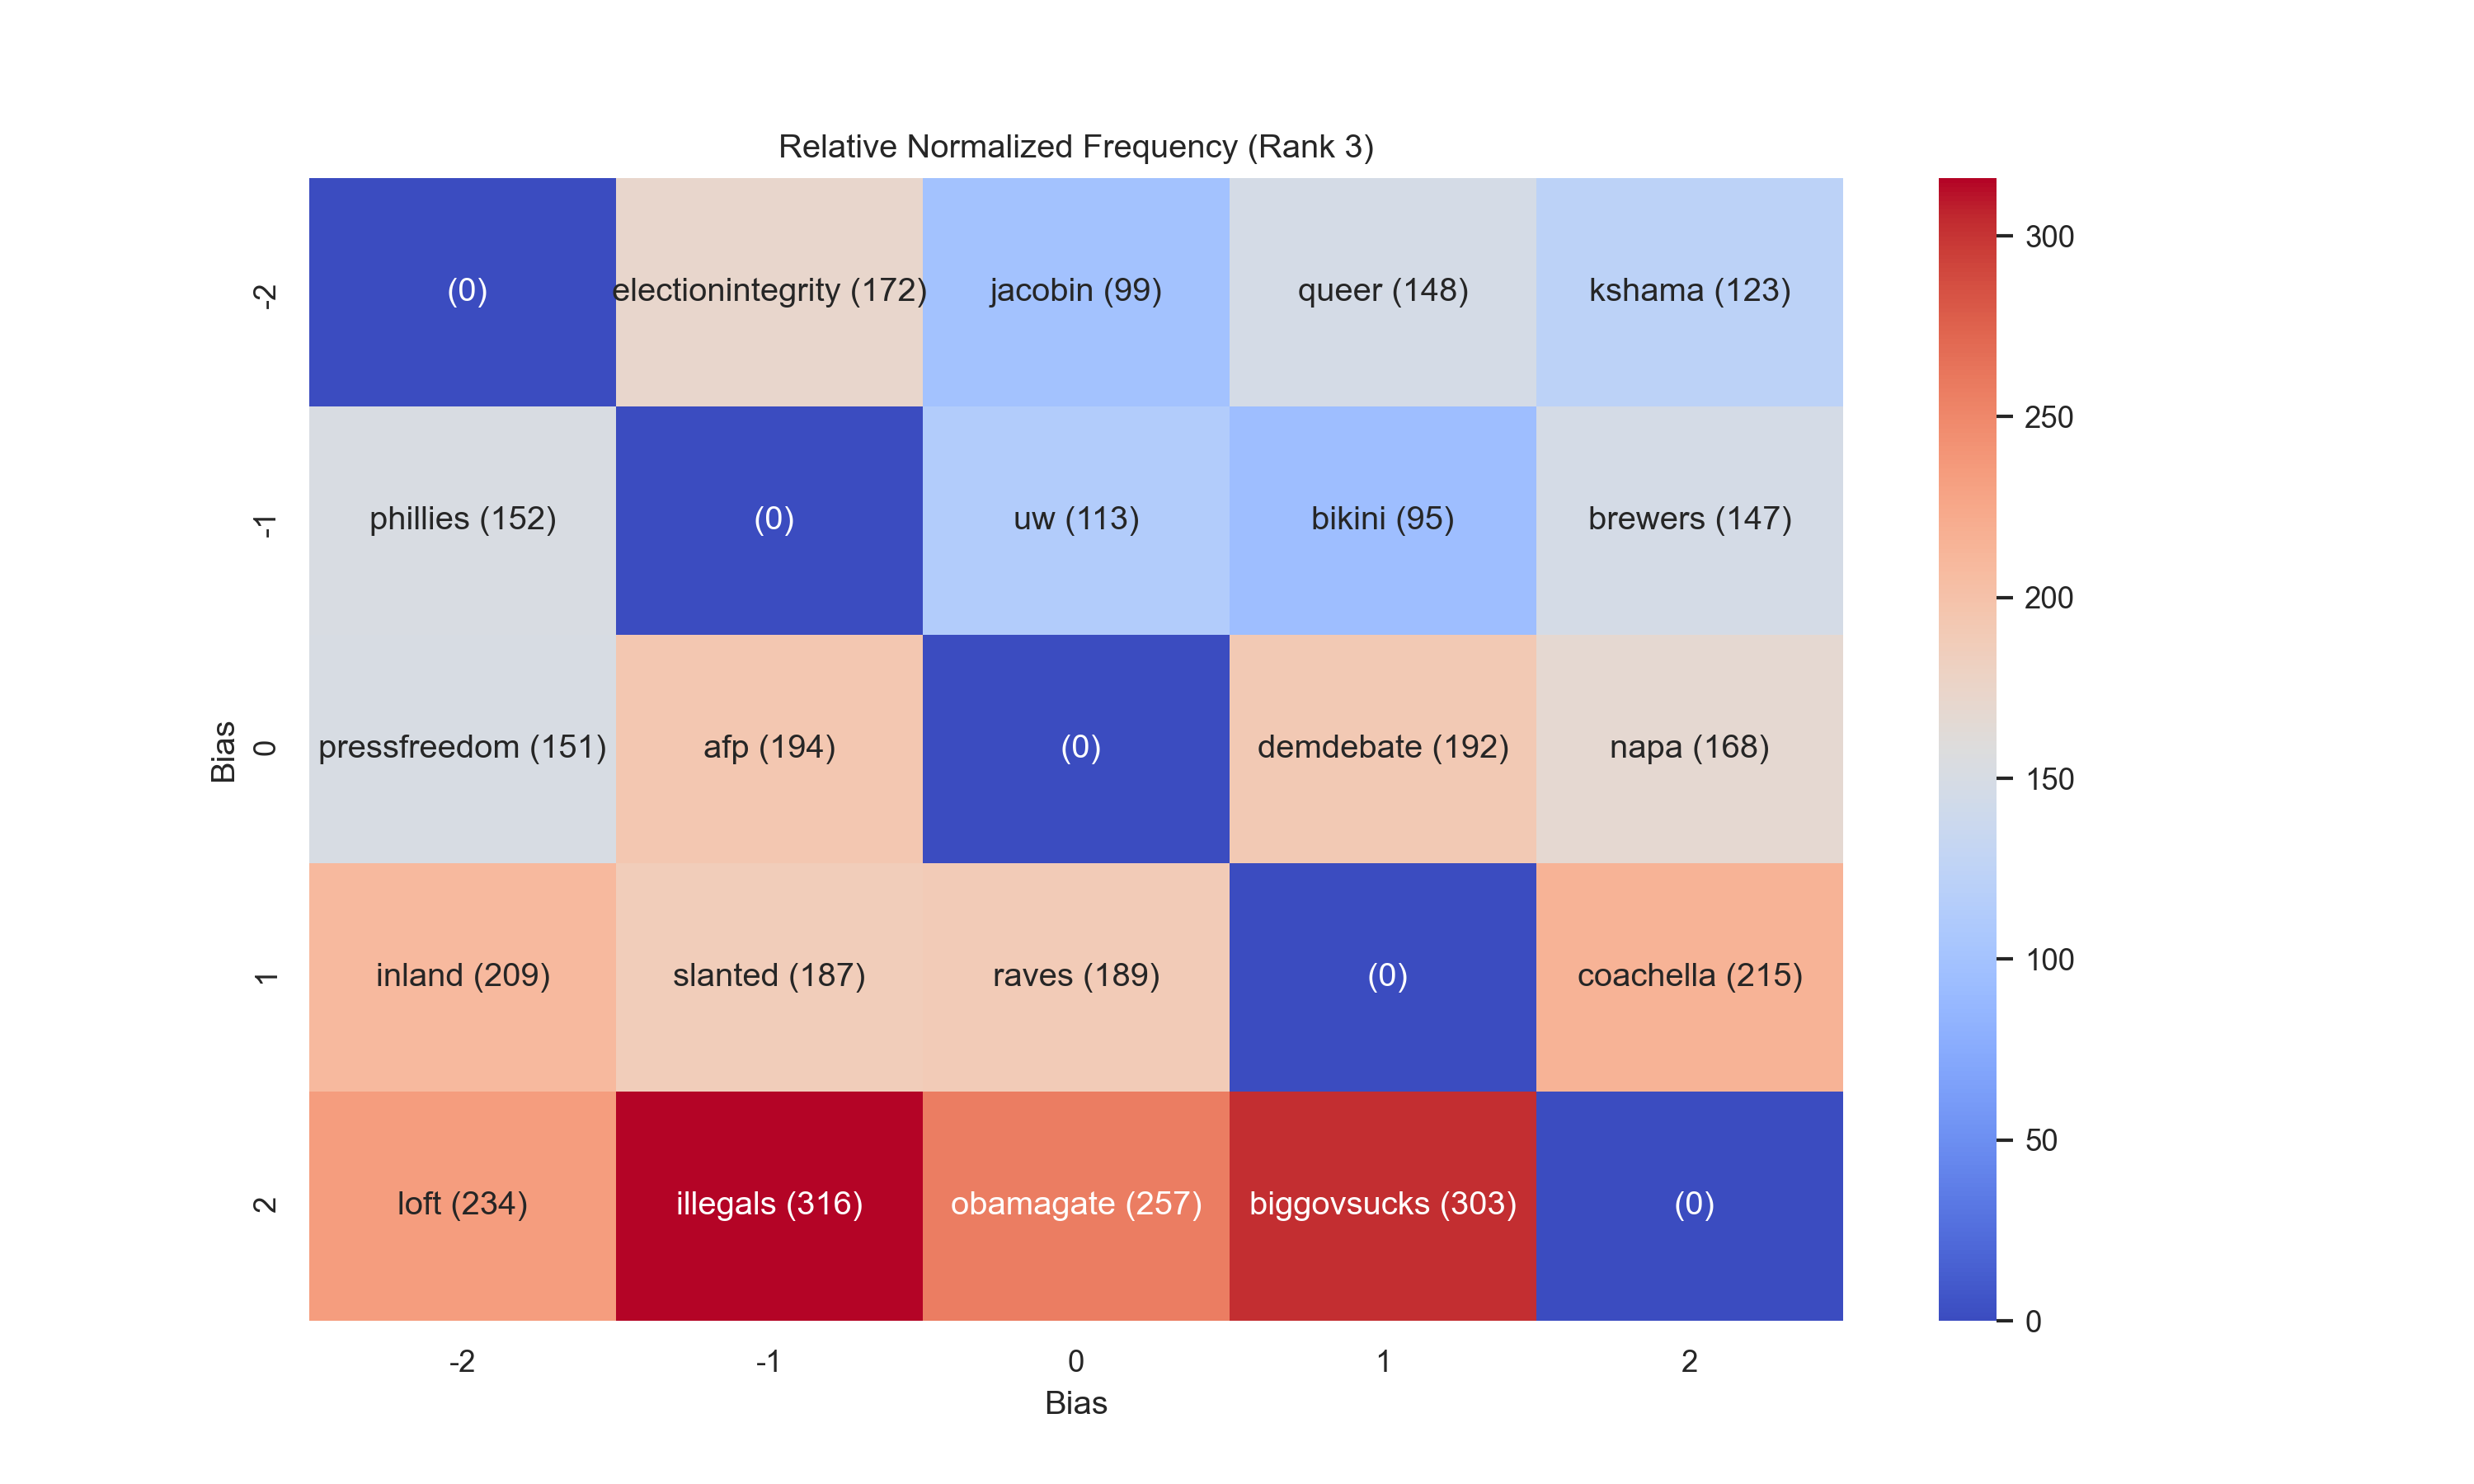
\includegraphics[width=0.6\textwidth]{figs/top_ten_rnf/rnf_t_rank_3.png}
\end{figure}
\end{center}

\pagebreak

\subsubsection{Rank 4}
\begin{center}

\CatchFileDef{\TTRNFTable}{figs/top_ten_rnf/table_rnf_t_rank_4.latex.txt}

\resizebox{\columnwidth}{!}
{
\TTRNFTable
}
\begin{figure}[h!]
  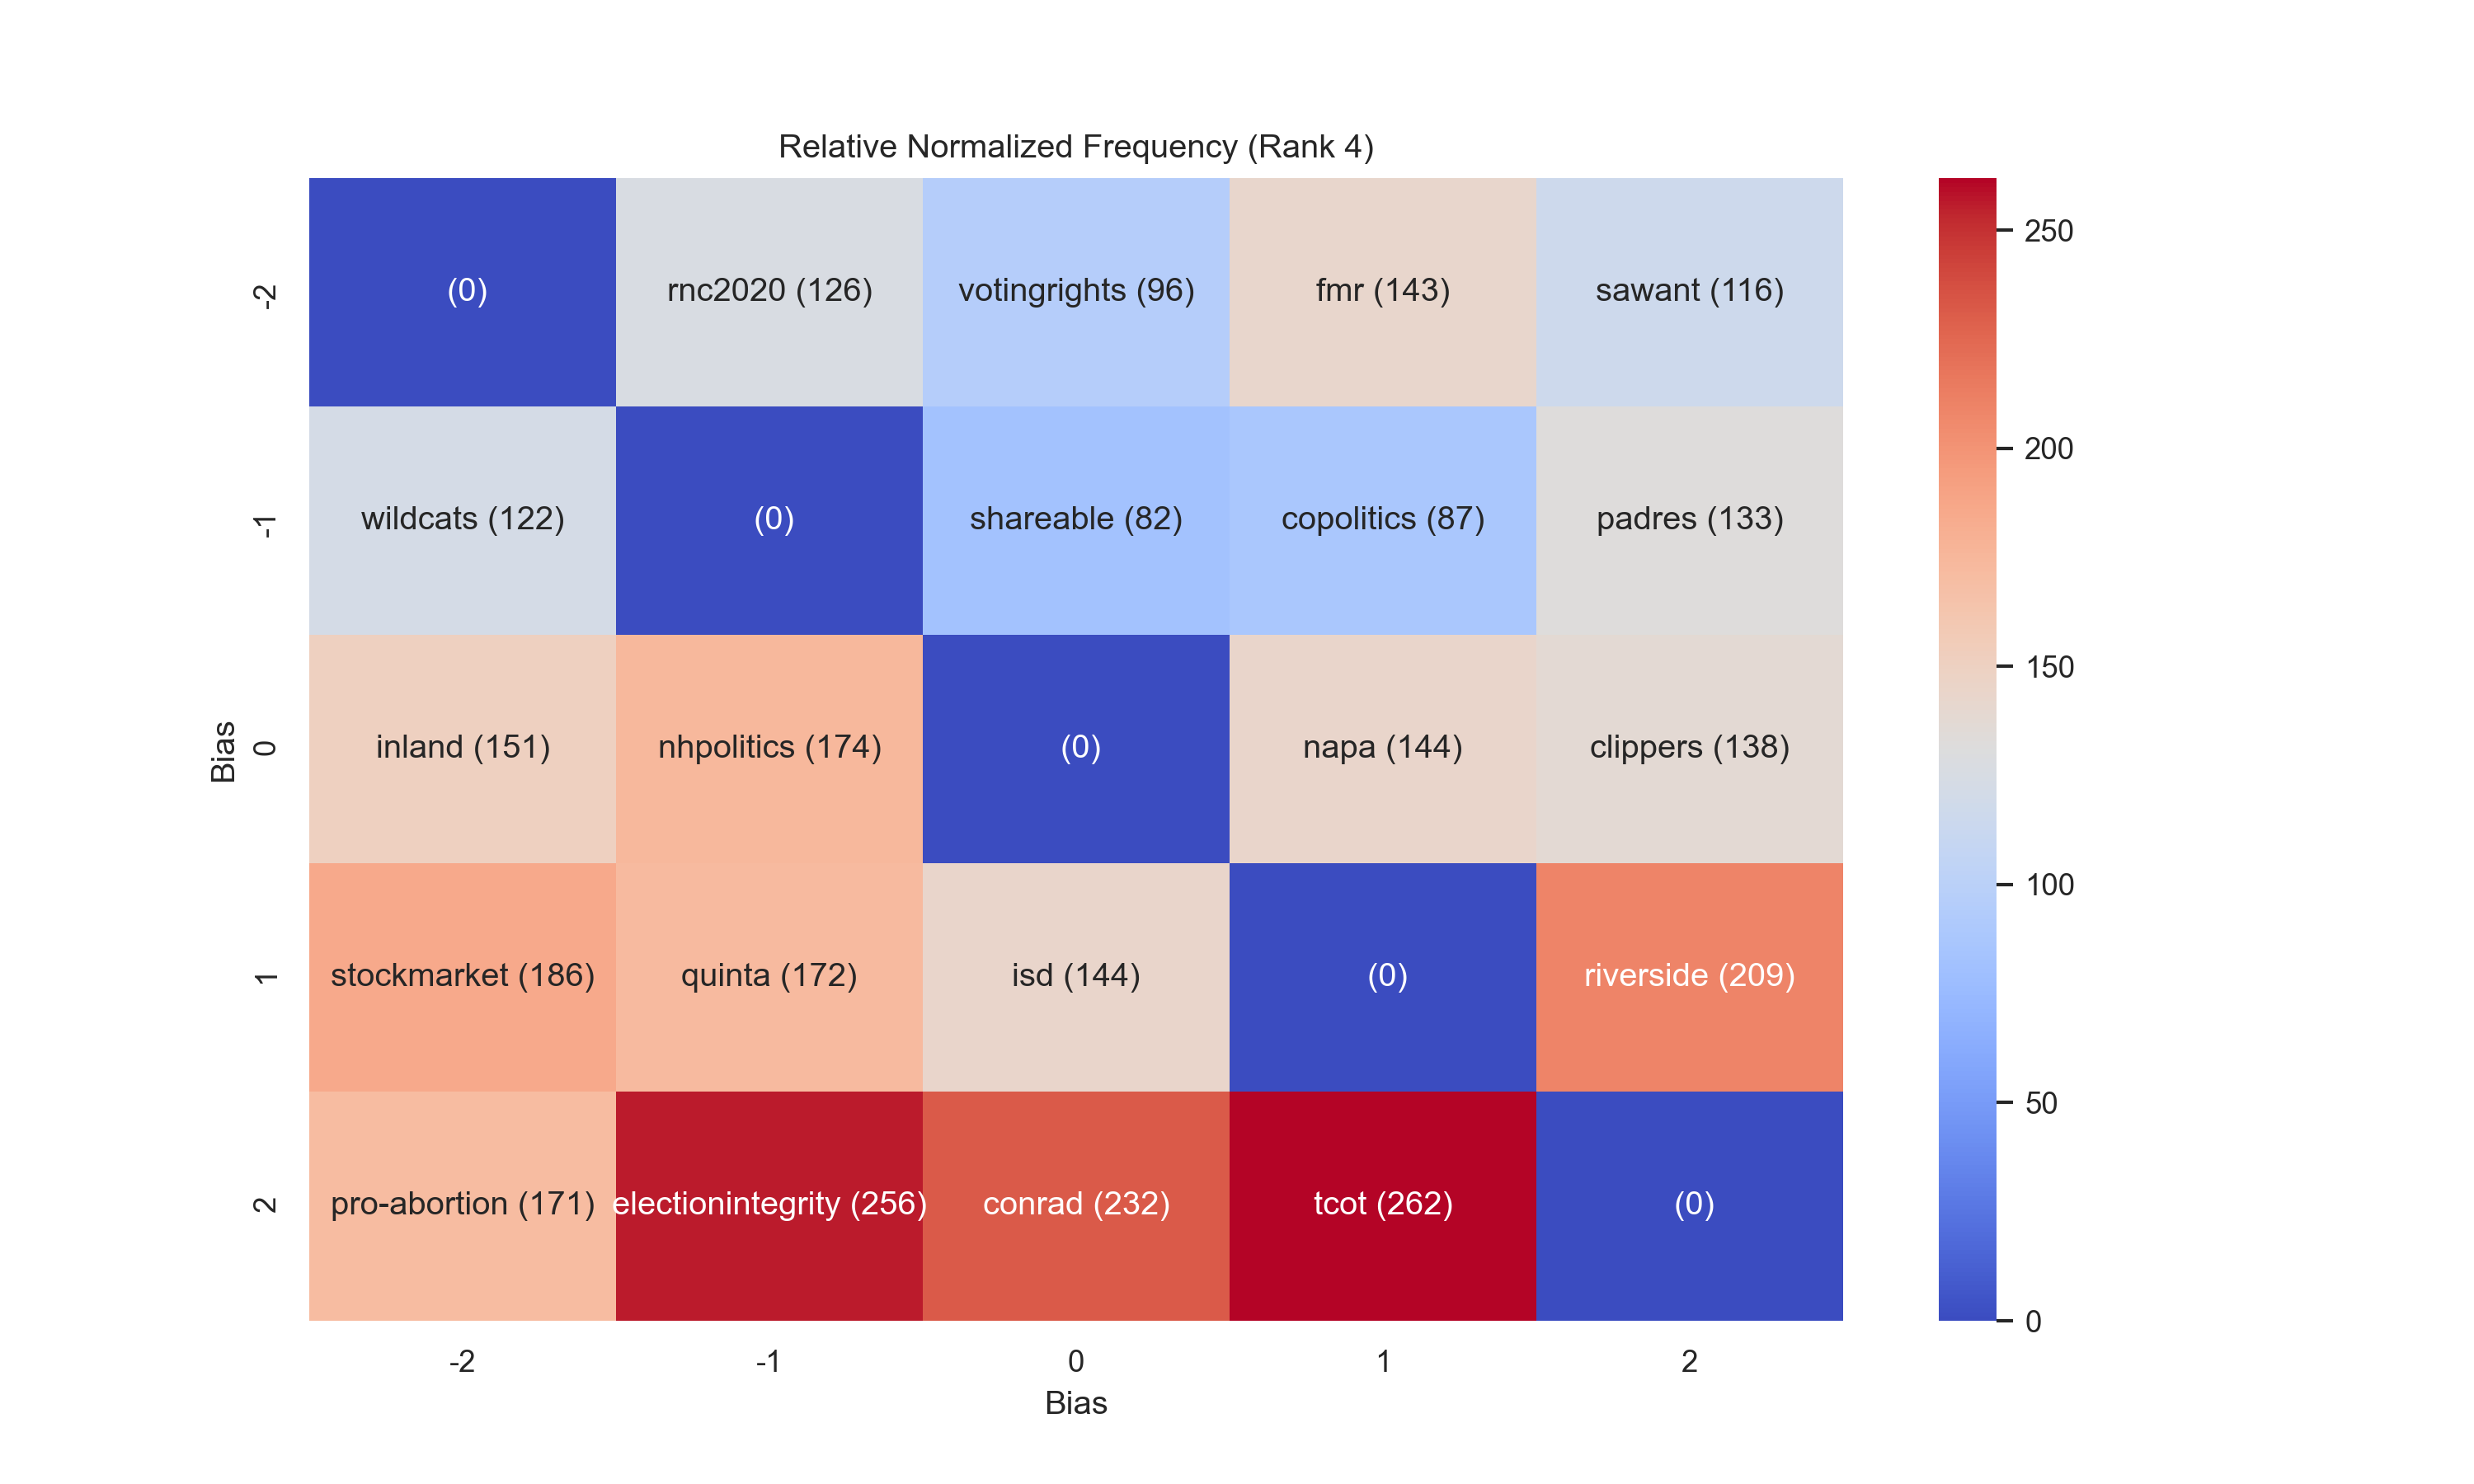
\includegraphics[width=0.6\textwidth]{figs/top_ten_rnf/rnf_t_rank_4.png}
\end{figure}
\end{center}

\subsubsection{Rank 5}
\begin{center}

\CatchFileDef{\TTRNFTable}{figs/top_ten_rnf/table_rnf_t_rank_5.latex.txt}

\resizebox{\columnwidth}{!}
{
\TTRNFTable
}
\begin{figure}[h!]
  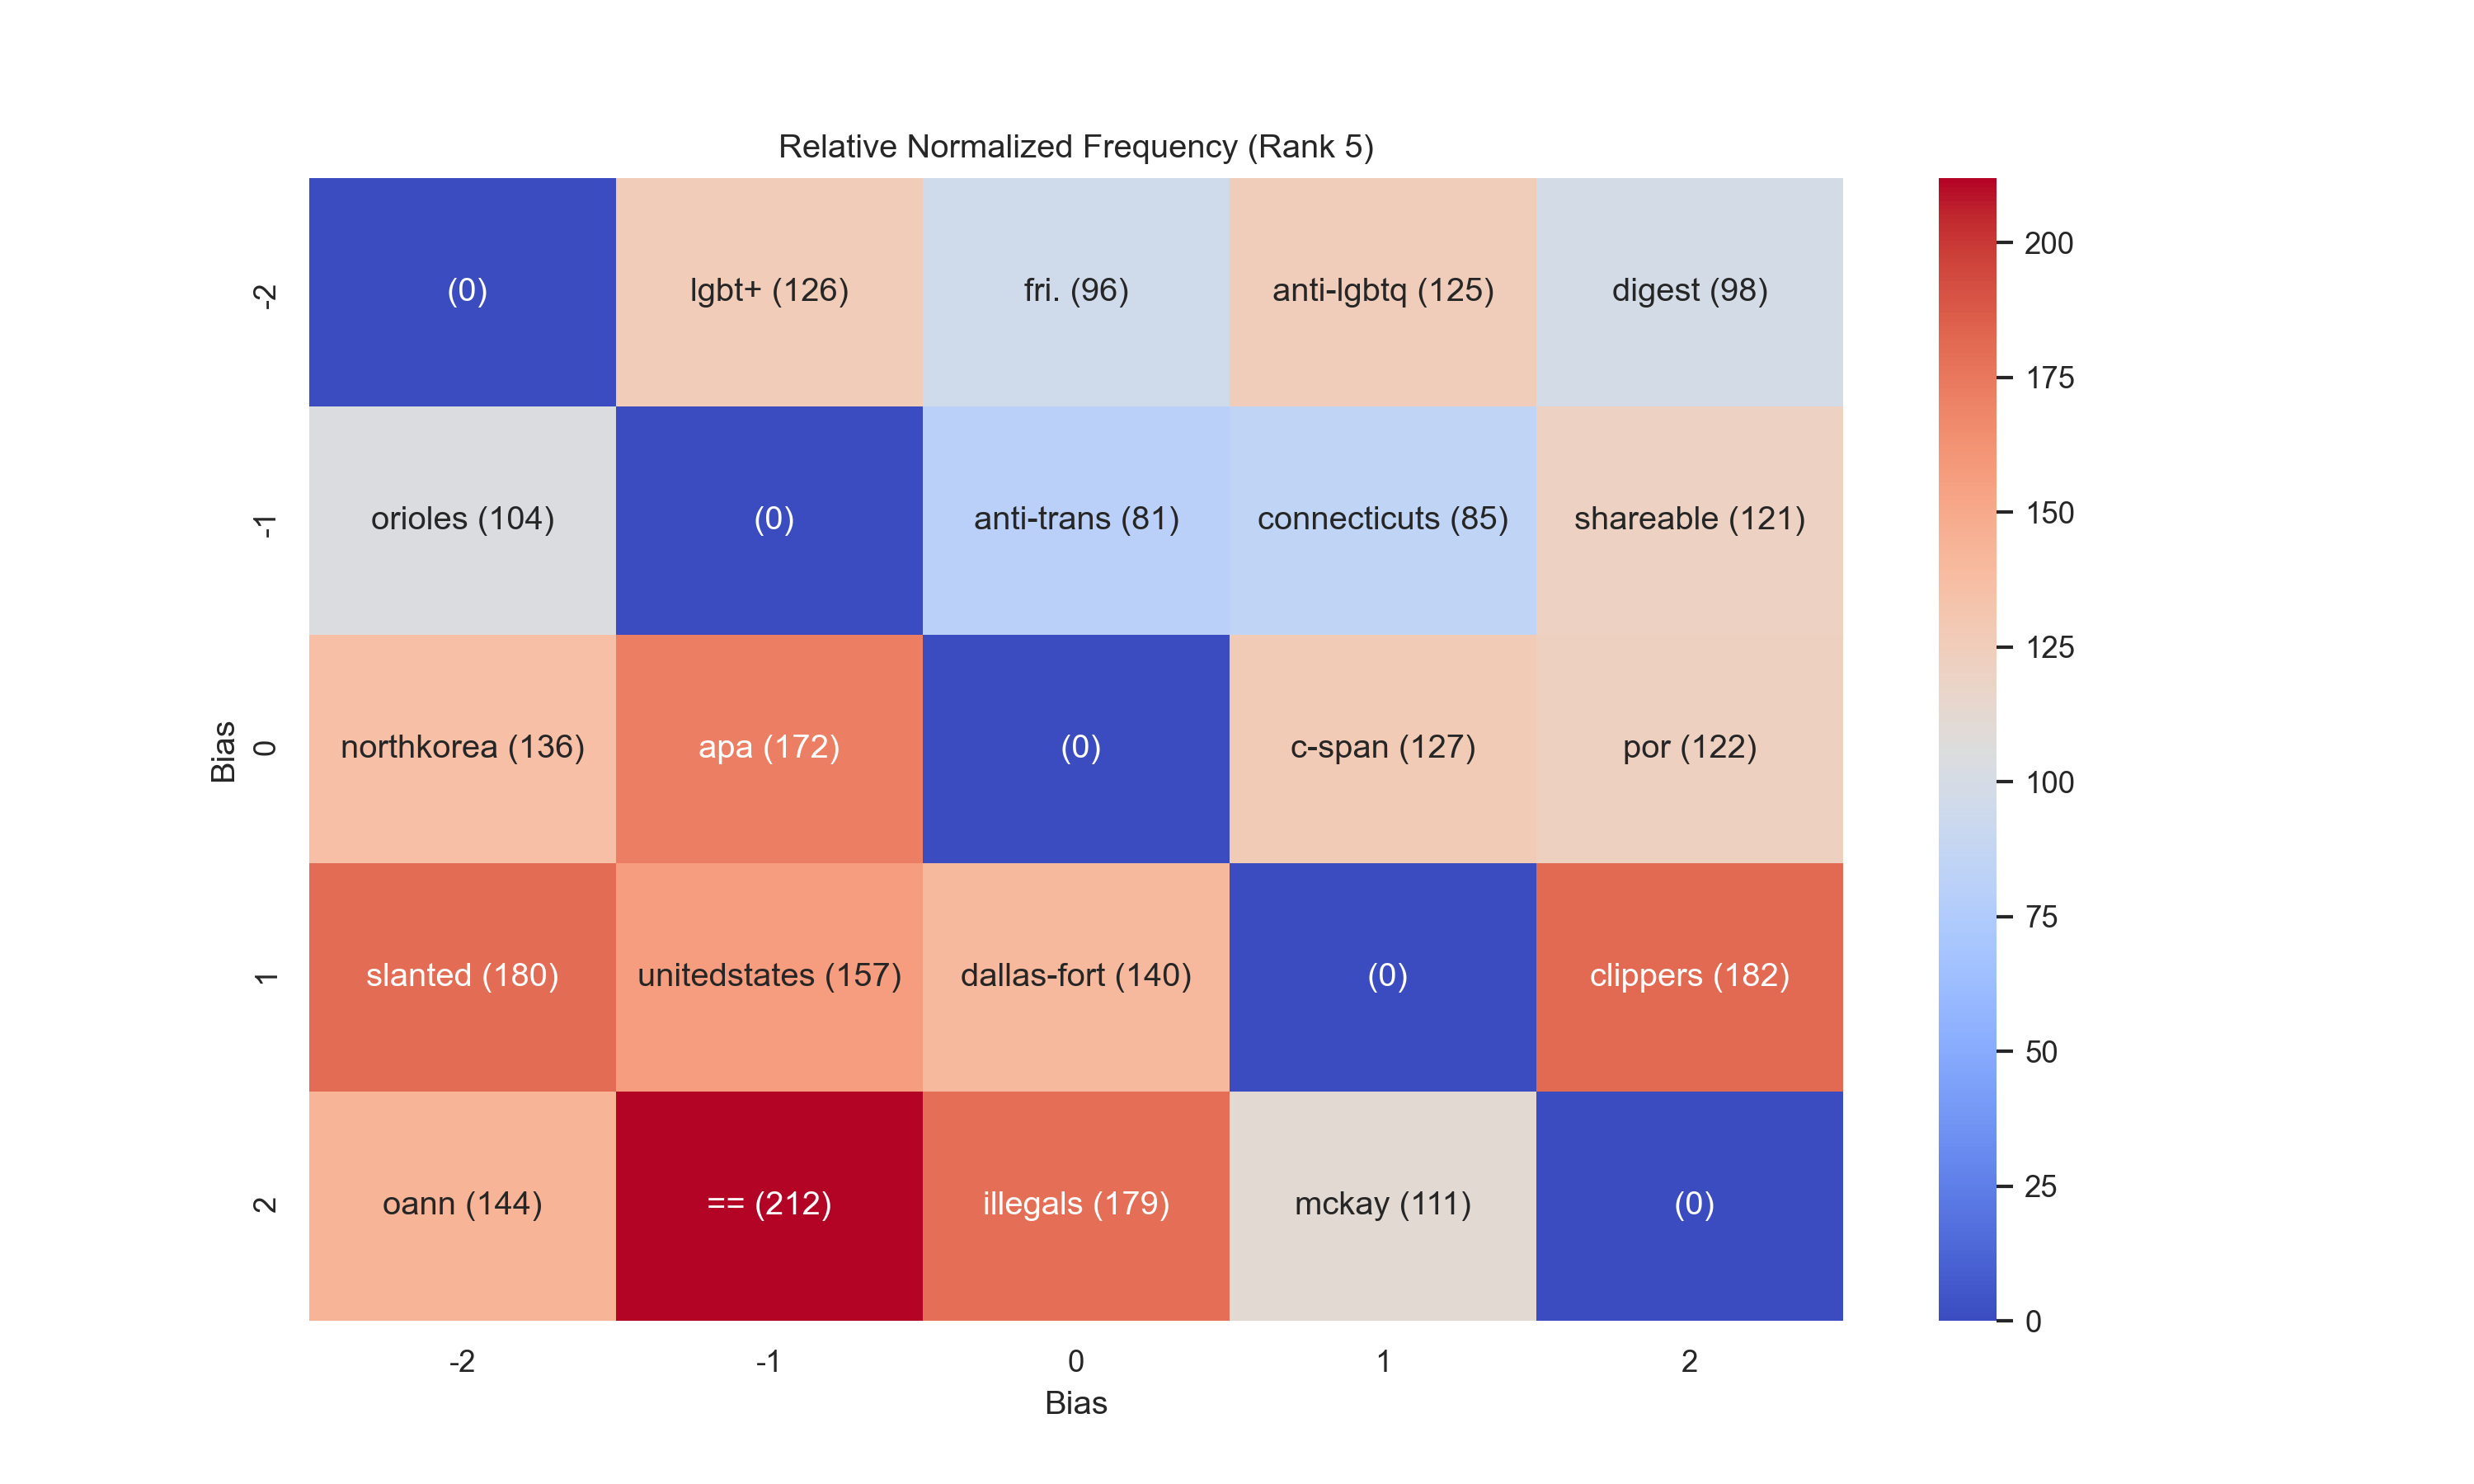
\includegraphics[width=0.6\textwidth]{figs/top_ten_rnf/rnf_t_rank_5.png}
\end{figure}
\end{center}

\pagebreak

\subsubsection{Rank 6}
\begin{center}

\CatchFileDef{\TTRNFTable}{figs/top_ten_rnf/table_rnf_t_rank_6.latex.txt}

\resizebox{\columnwidth}{!}
{
\TTRNFTable
}
\begin{figure}[h!]
  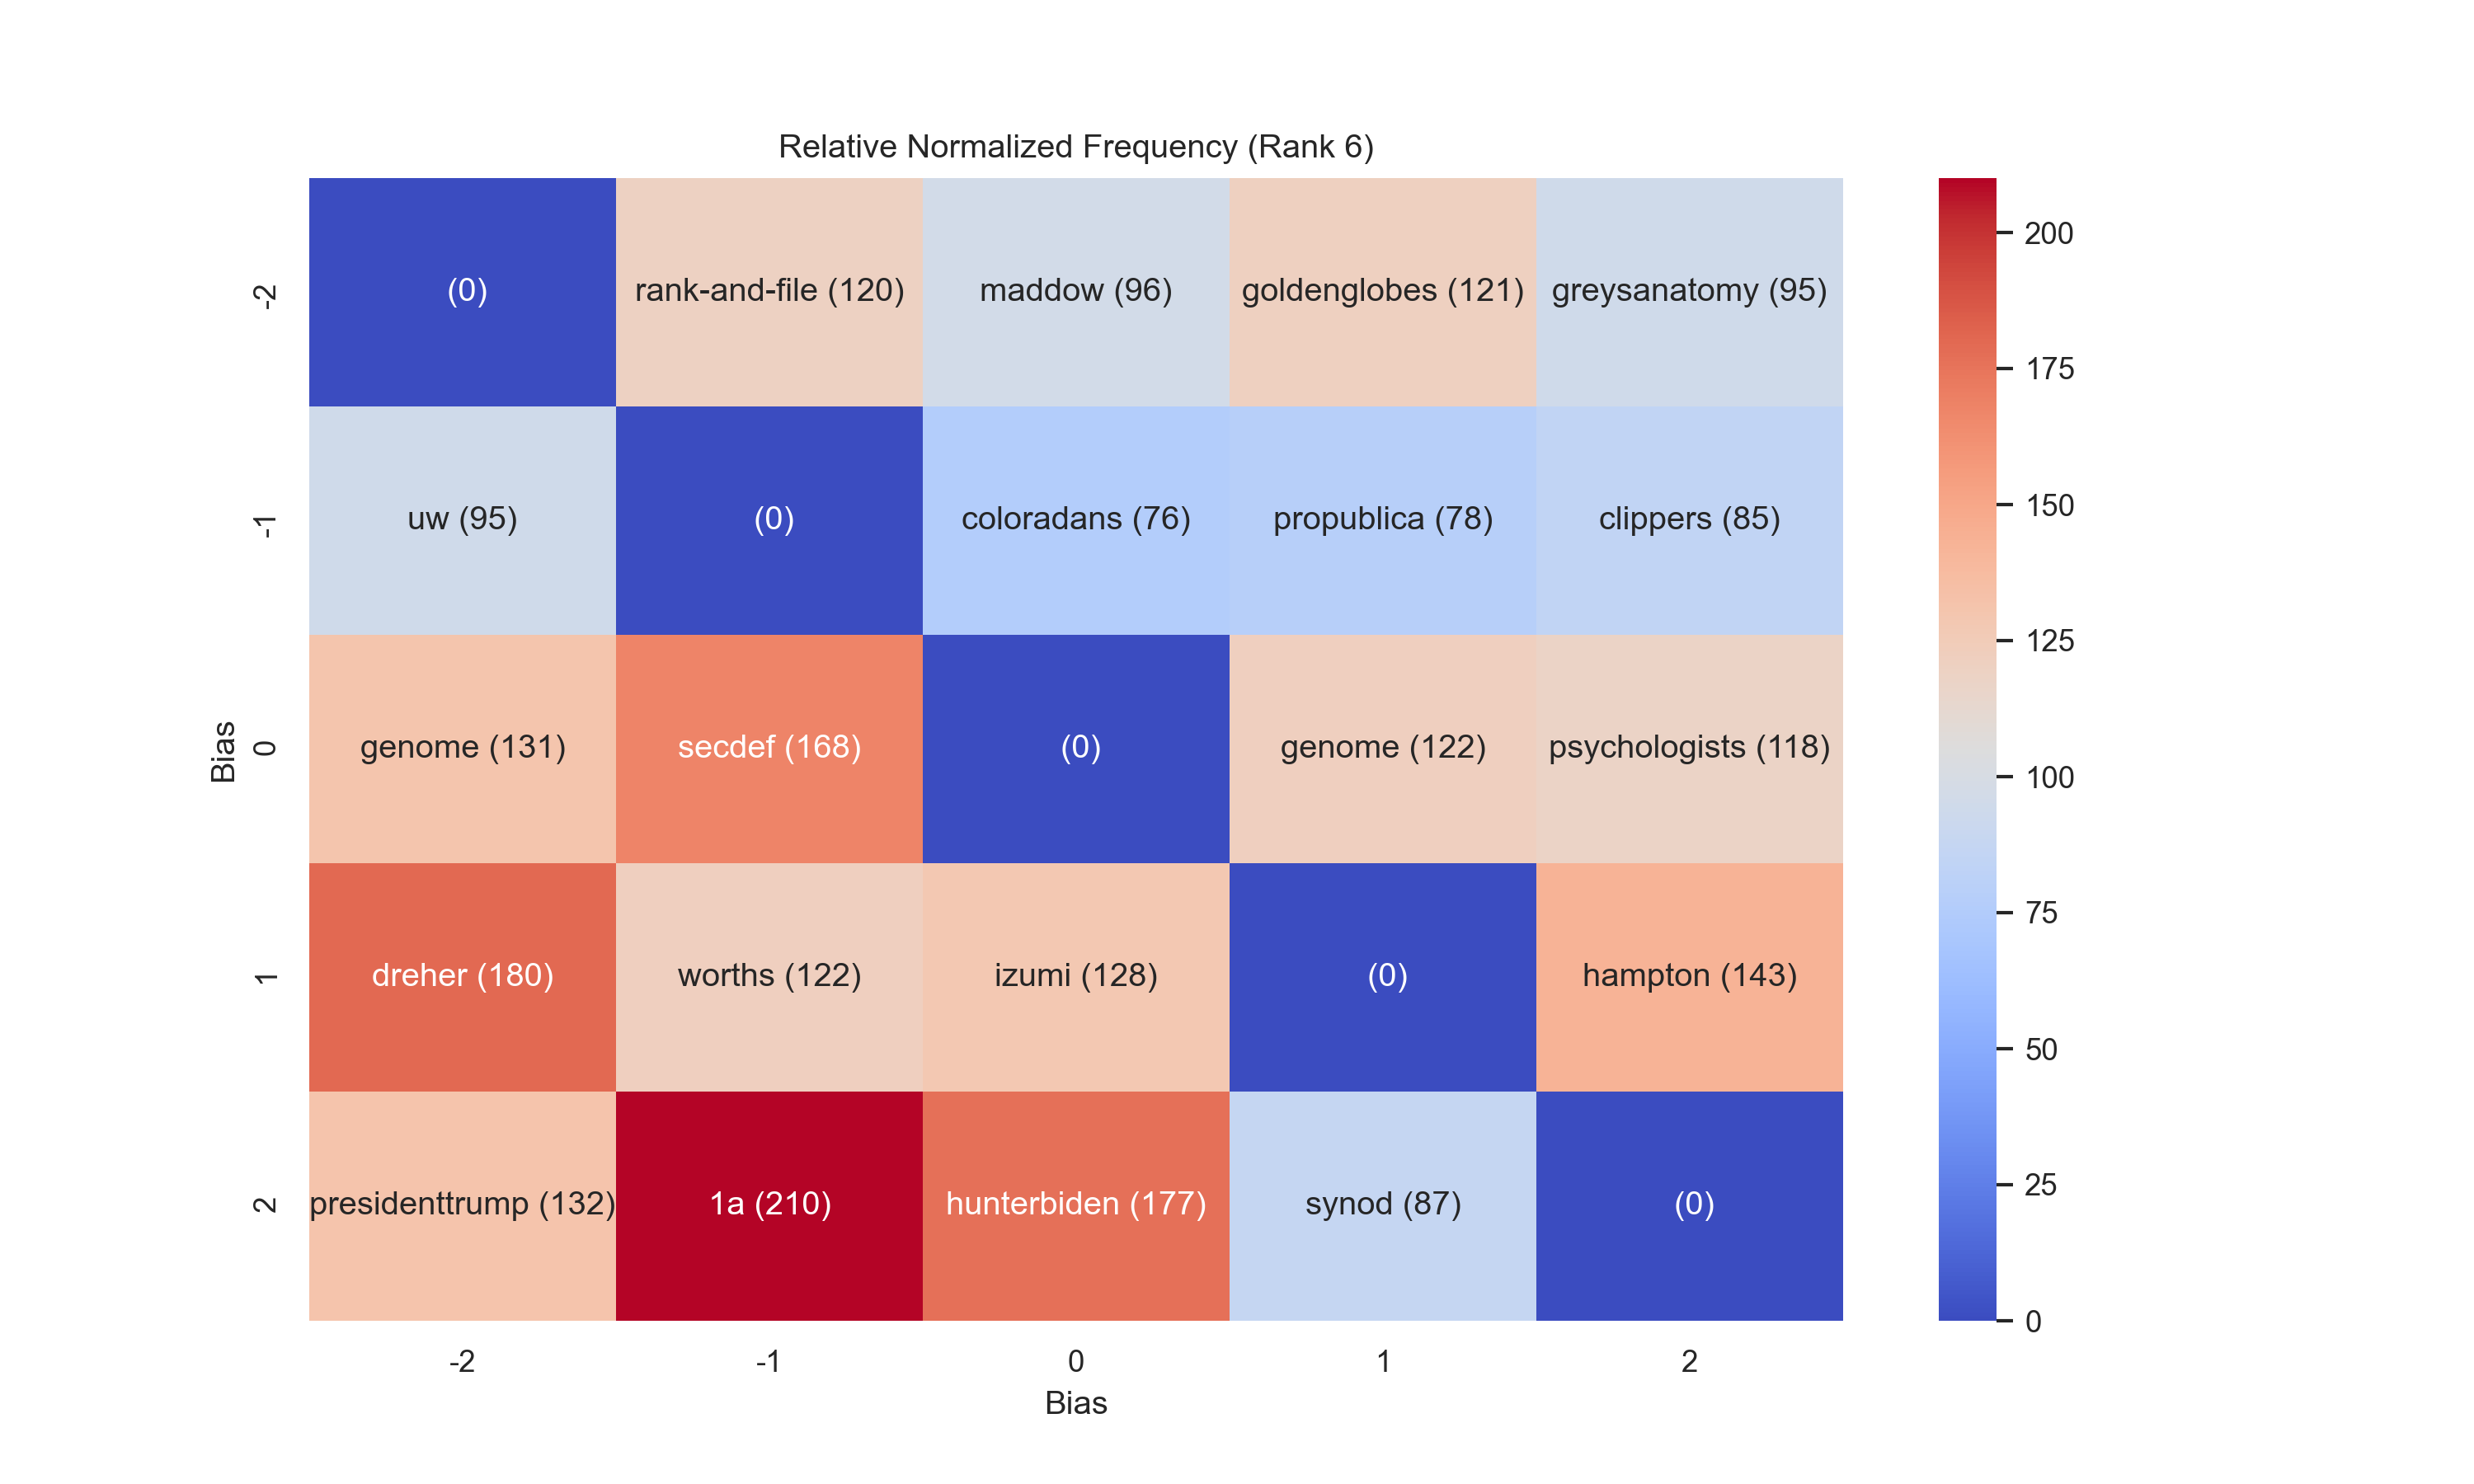
\includegraphics[width=0.6\textwidth]{figs/top_ten_rnf/rnf_t_rank_6.png}
\end{figure}
\end{center}

\subsubsection{Rank 7}
\begin{center}

\CatchFileDef{\TTRNFTable}{figs/top_ten_rnf/table_rnf_t_rank_7.latex.txt}

\resizebox{\columnwidth}{!}
{
\TTRNFTable
}
\begin{figure}[h!]
  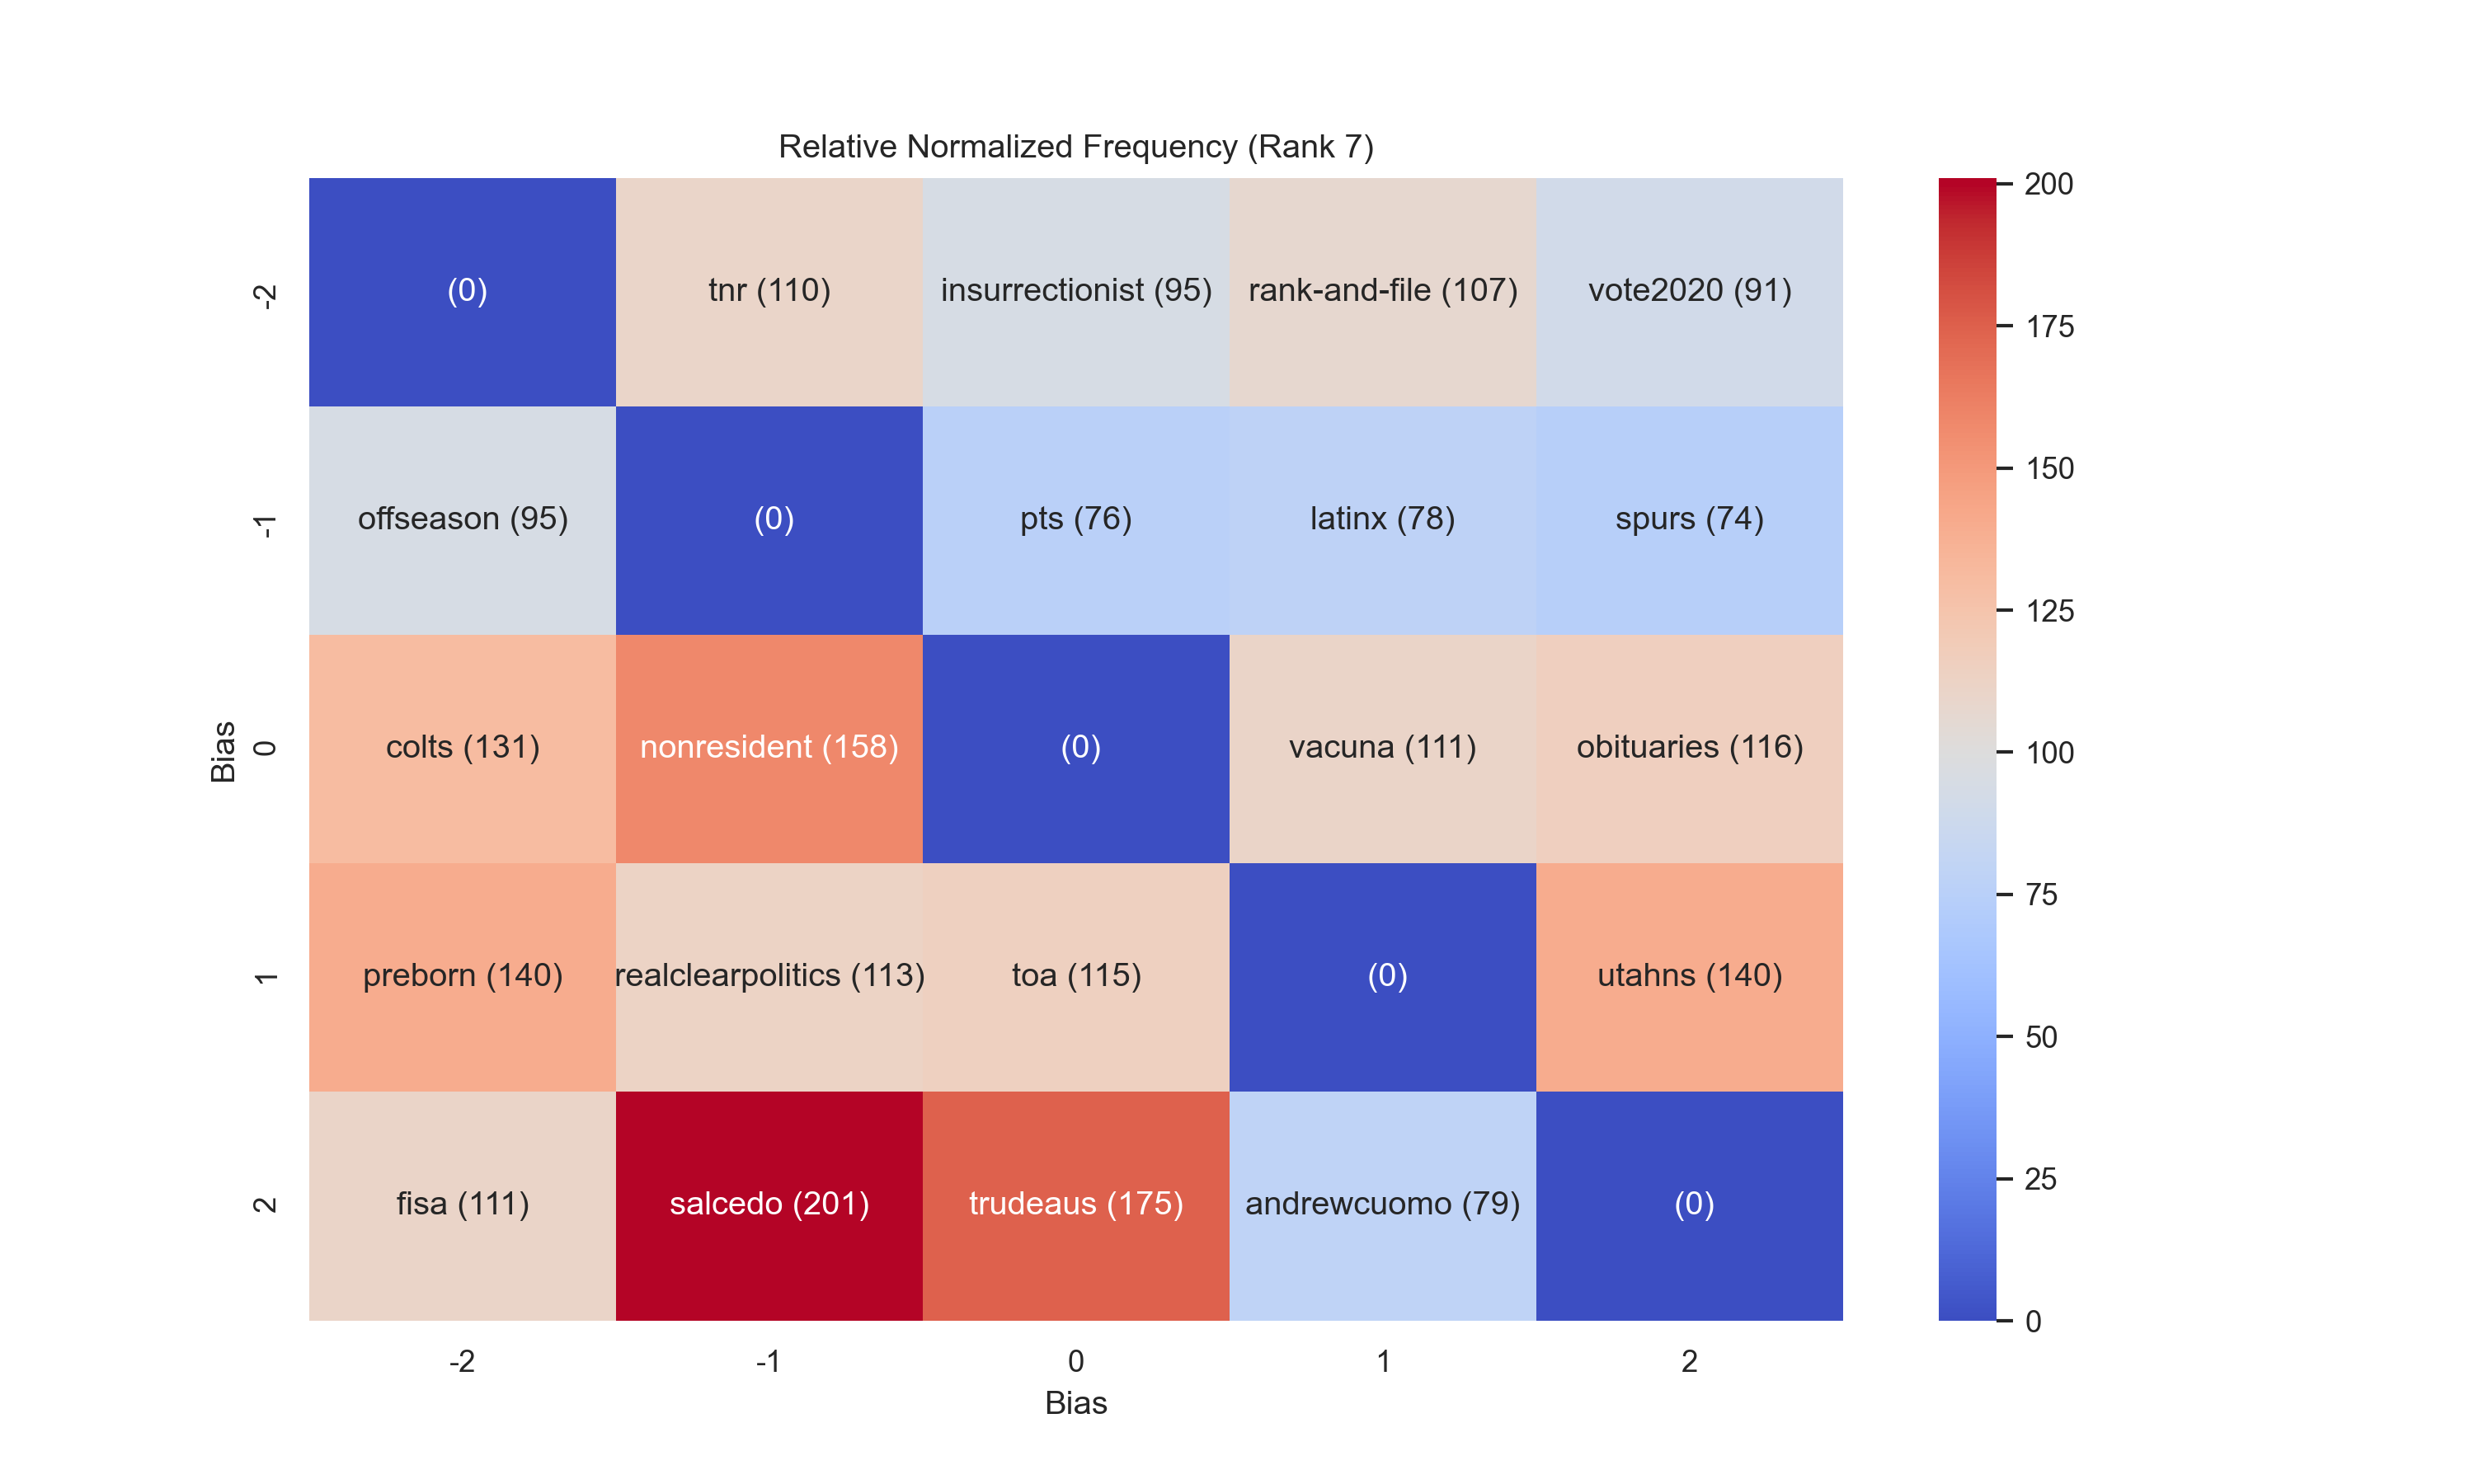
\includegraphics[width=0.6\textwidth]{figs/top_ten_rnf/rnf_t_rank_7.png}
\end{figure}
\end{center}

\pagebreak

\subsubsection{Rank 8}
\begin{center}

\CatchFileDef{\TTRNFTable}{figs/top_ten_rnf/table_rnf_t_rank_8.latex.txt}

\resizebox{\columnwidth}{!}
{
\TTRNFTable
}
\begin{figure}[h!]
  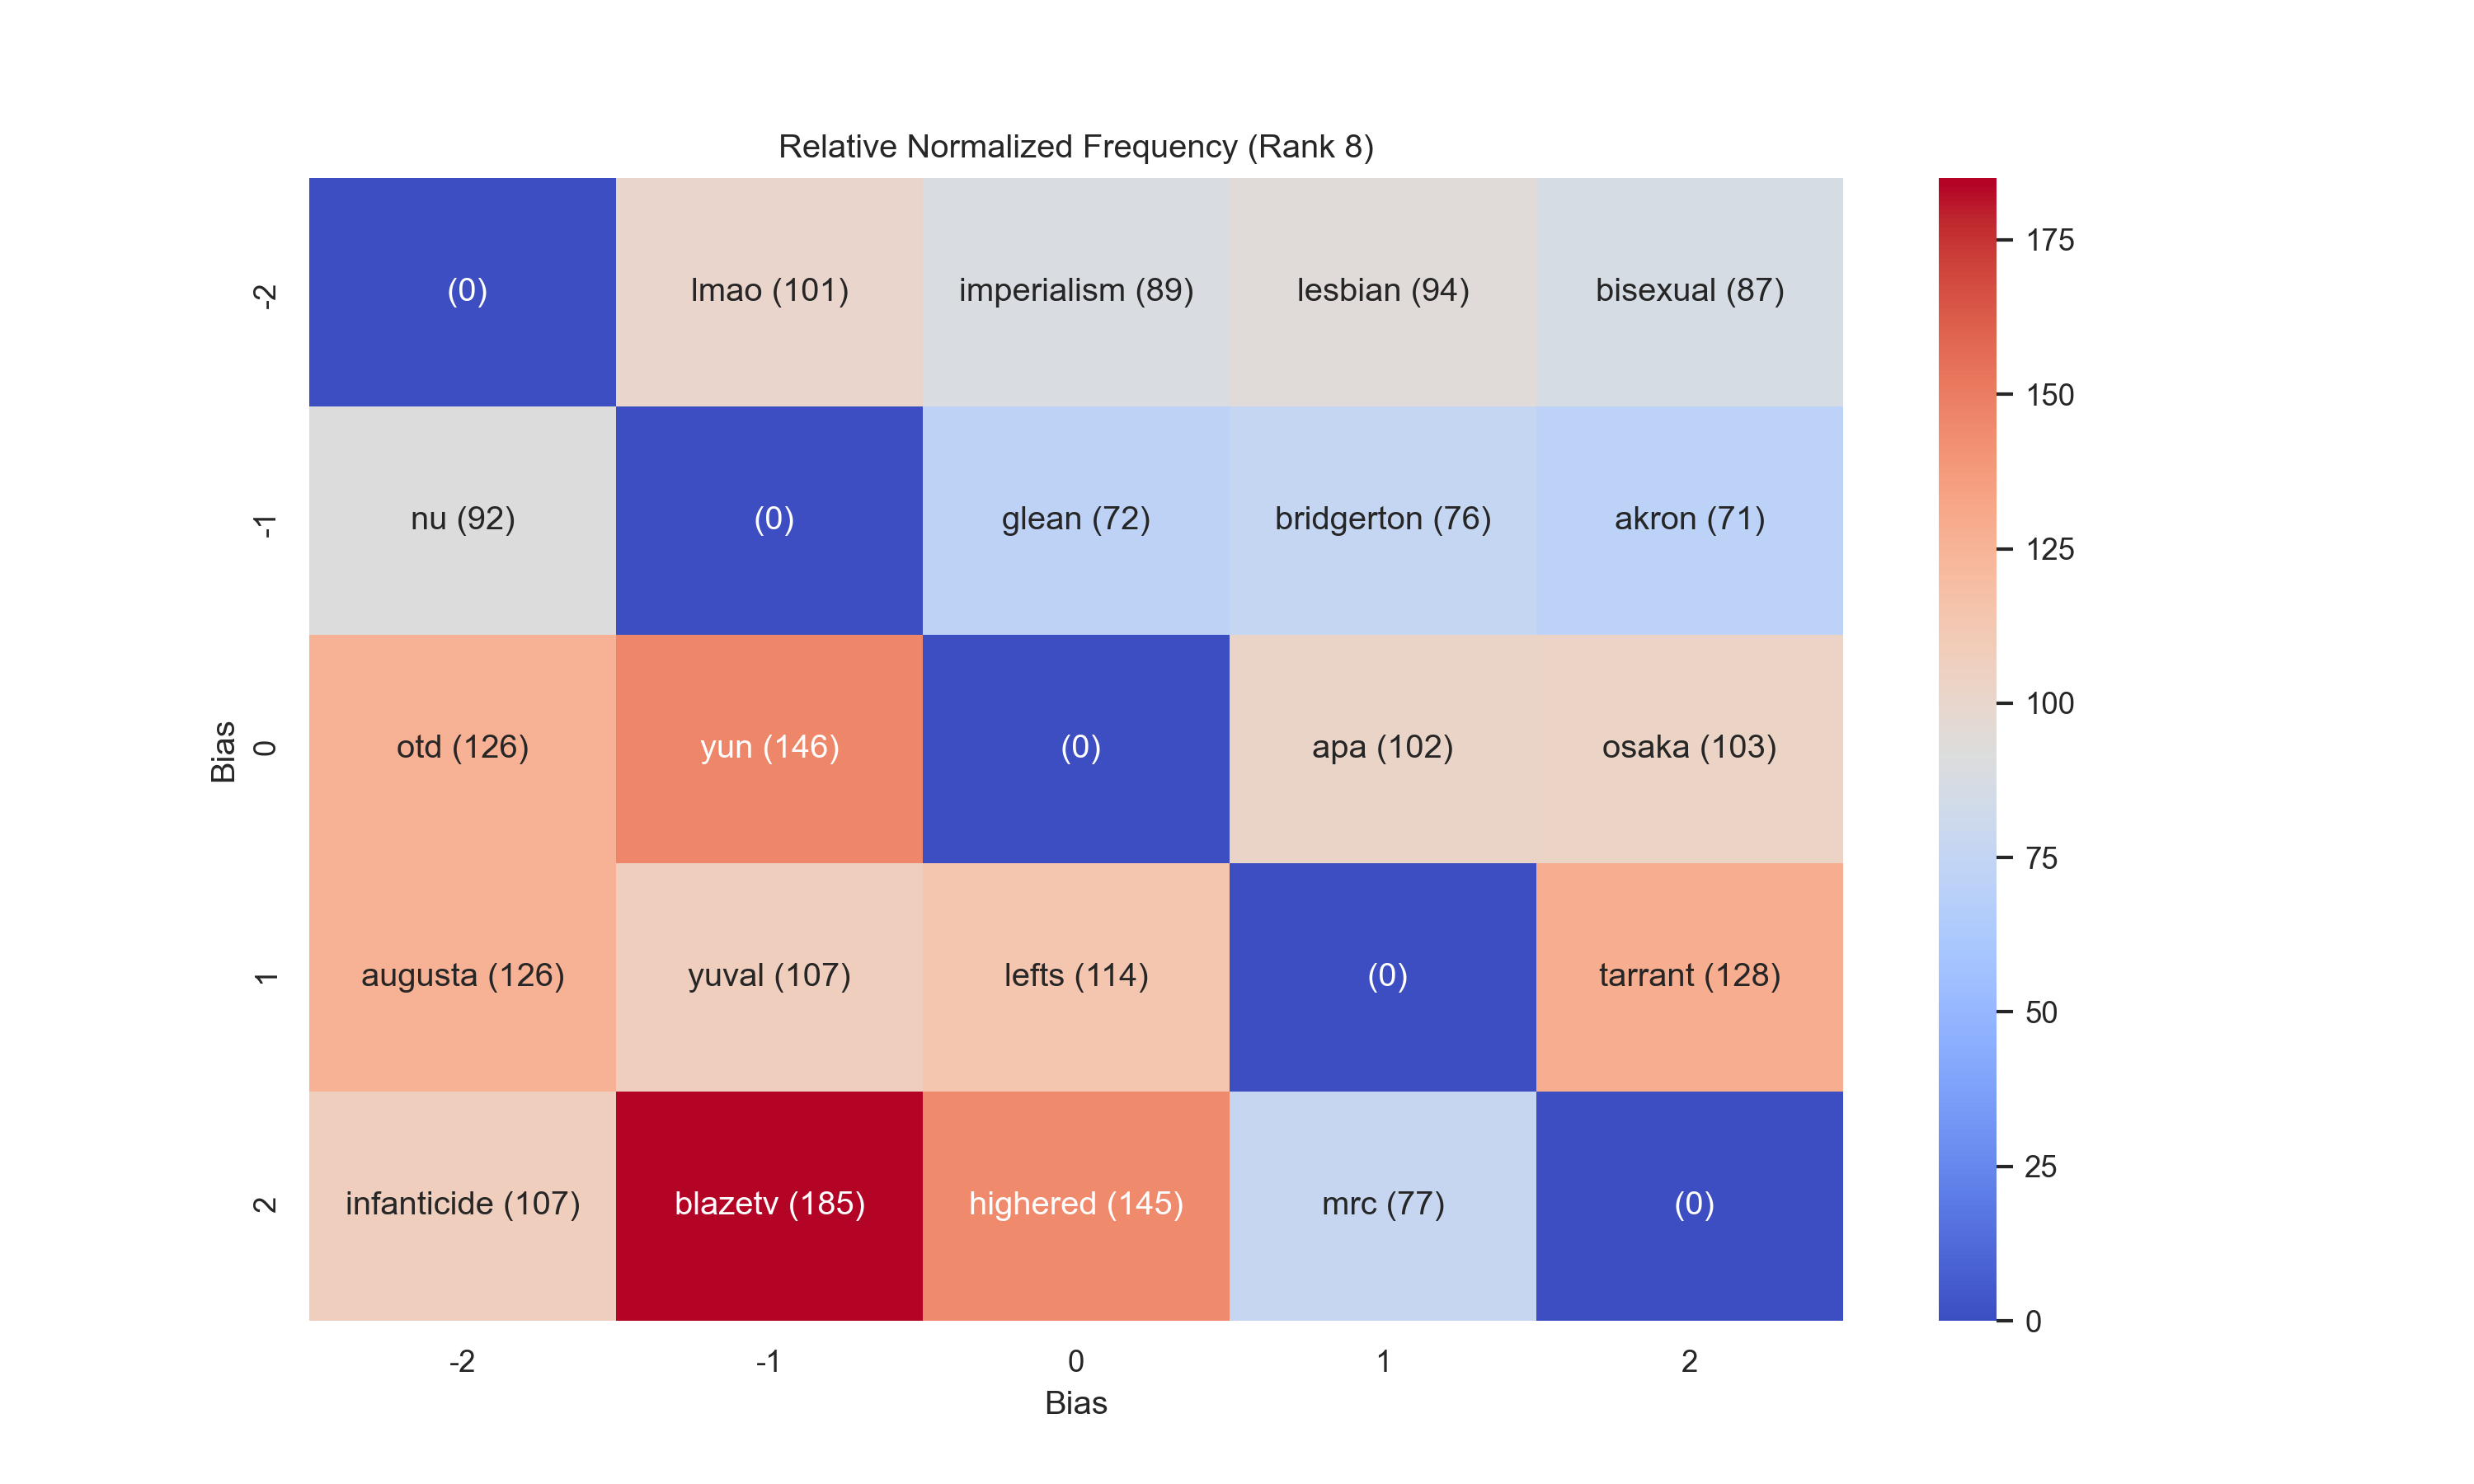
\includegraphics[width=0.6\textwidth]{figs/top_ten_rnf/rnf_t_rank_8.png}
\end{figure}
\end{center}

\subsubsection{Rank 9}
\begin{center}

\CatchFileDef{\TTRNFTable}{figs/top_ten_rnf/table_rnf_t_rank_9.latex.txt}

\resizebox{\columnwidth}{!}
{
\TTRNFTable
}
\begin{figure}[h!]
  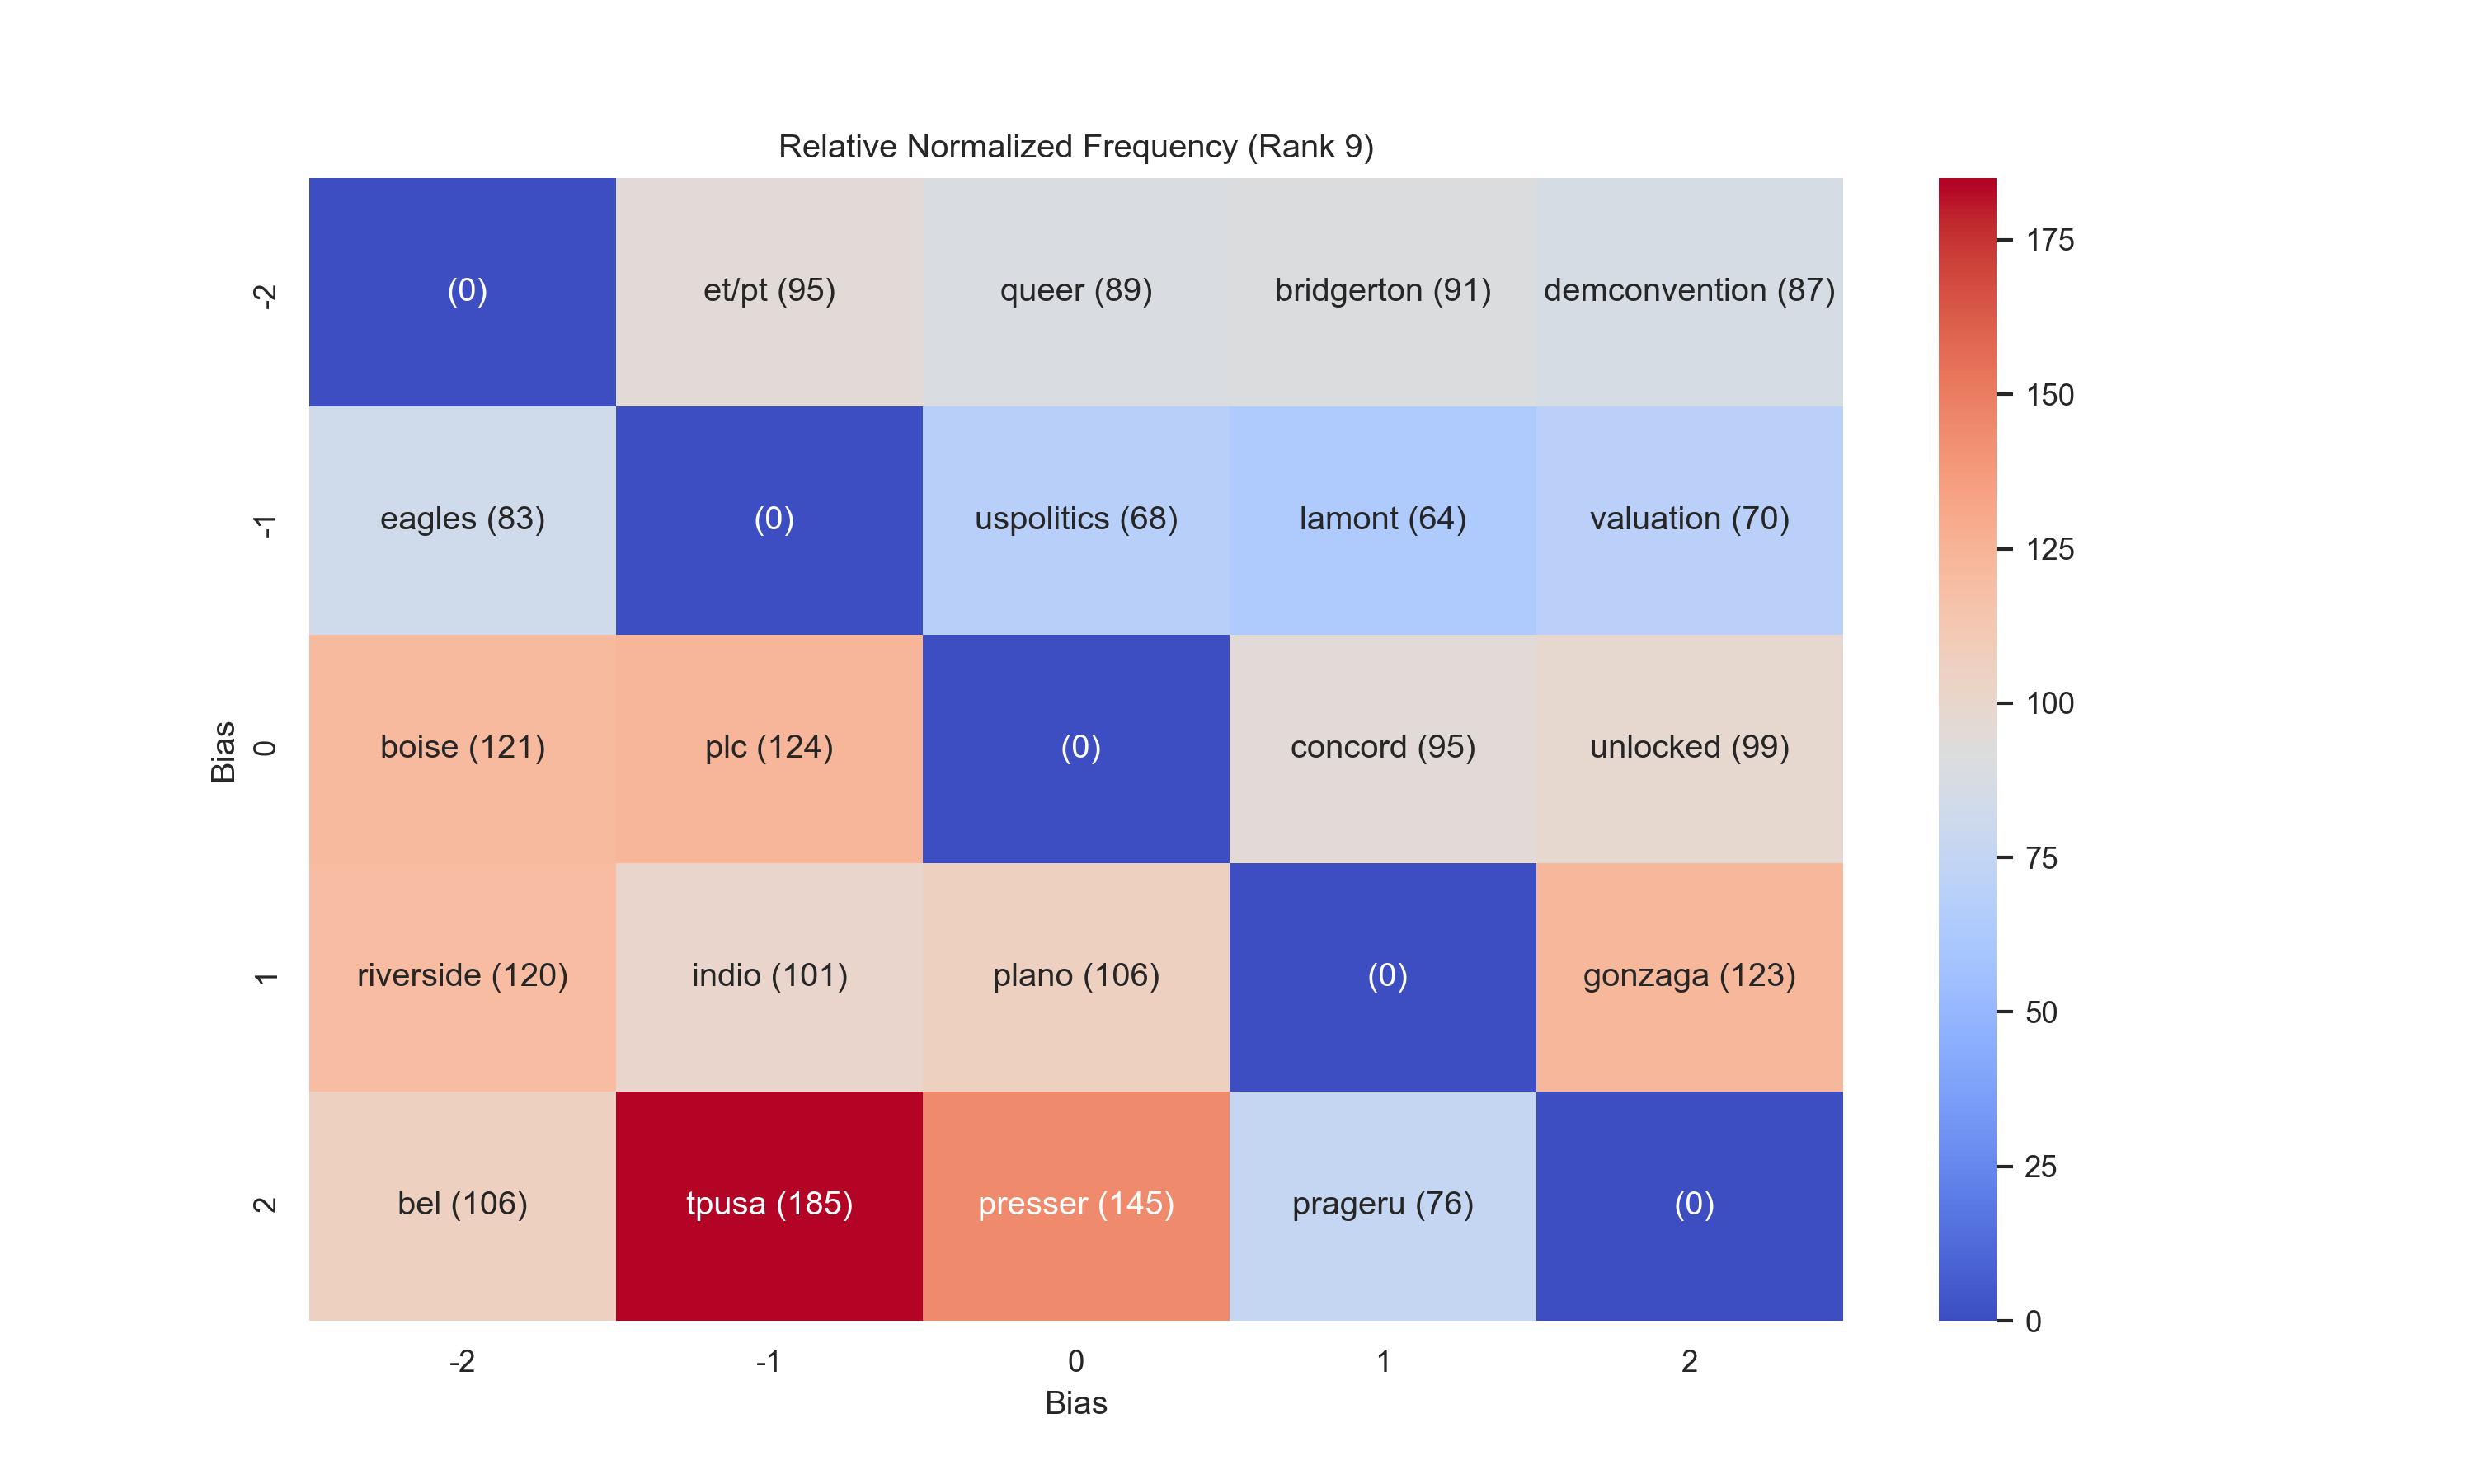
\includegraphics[width=0.6\textwidth]{figs/top_ten_rnf/rnf_t_rank_9.png}
\end{figure}
\end{center}

\pagebreak

\subsection{Top Ten Common Words Based on Relative Normalized Frequency}
\subsubsection{Rank 0}
\begin{center}

\CatchFileDef{\TTRNFTable}{figs/top_ten_rnf/table_rnf_w_rank_0.latex.txt}

\resizebox{\columnwidth}{!}
{
\TTRNFTable
}
\begin{figure}[h!]
  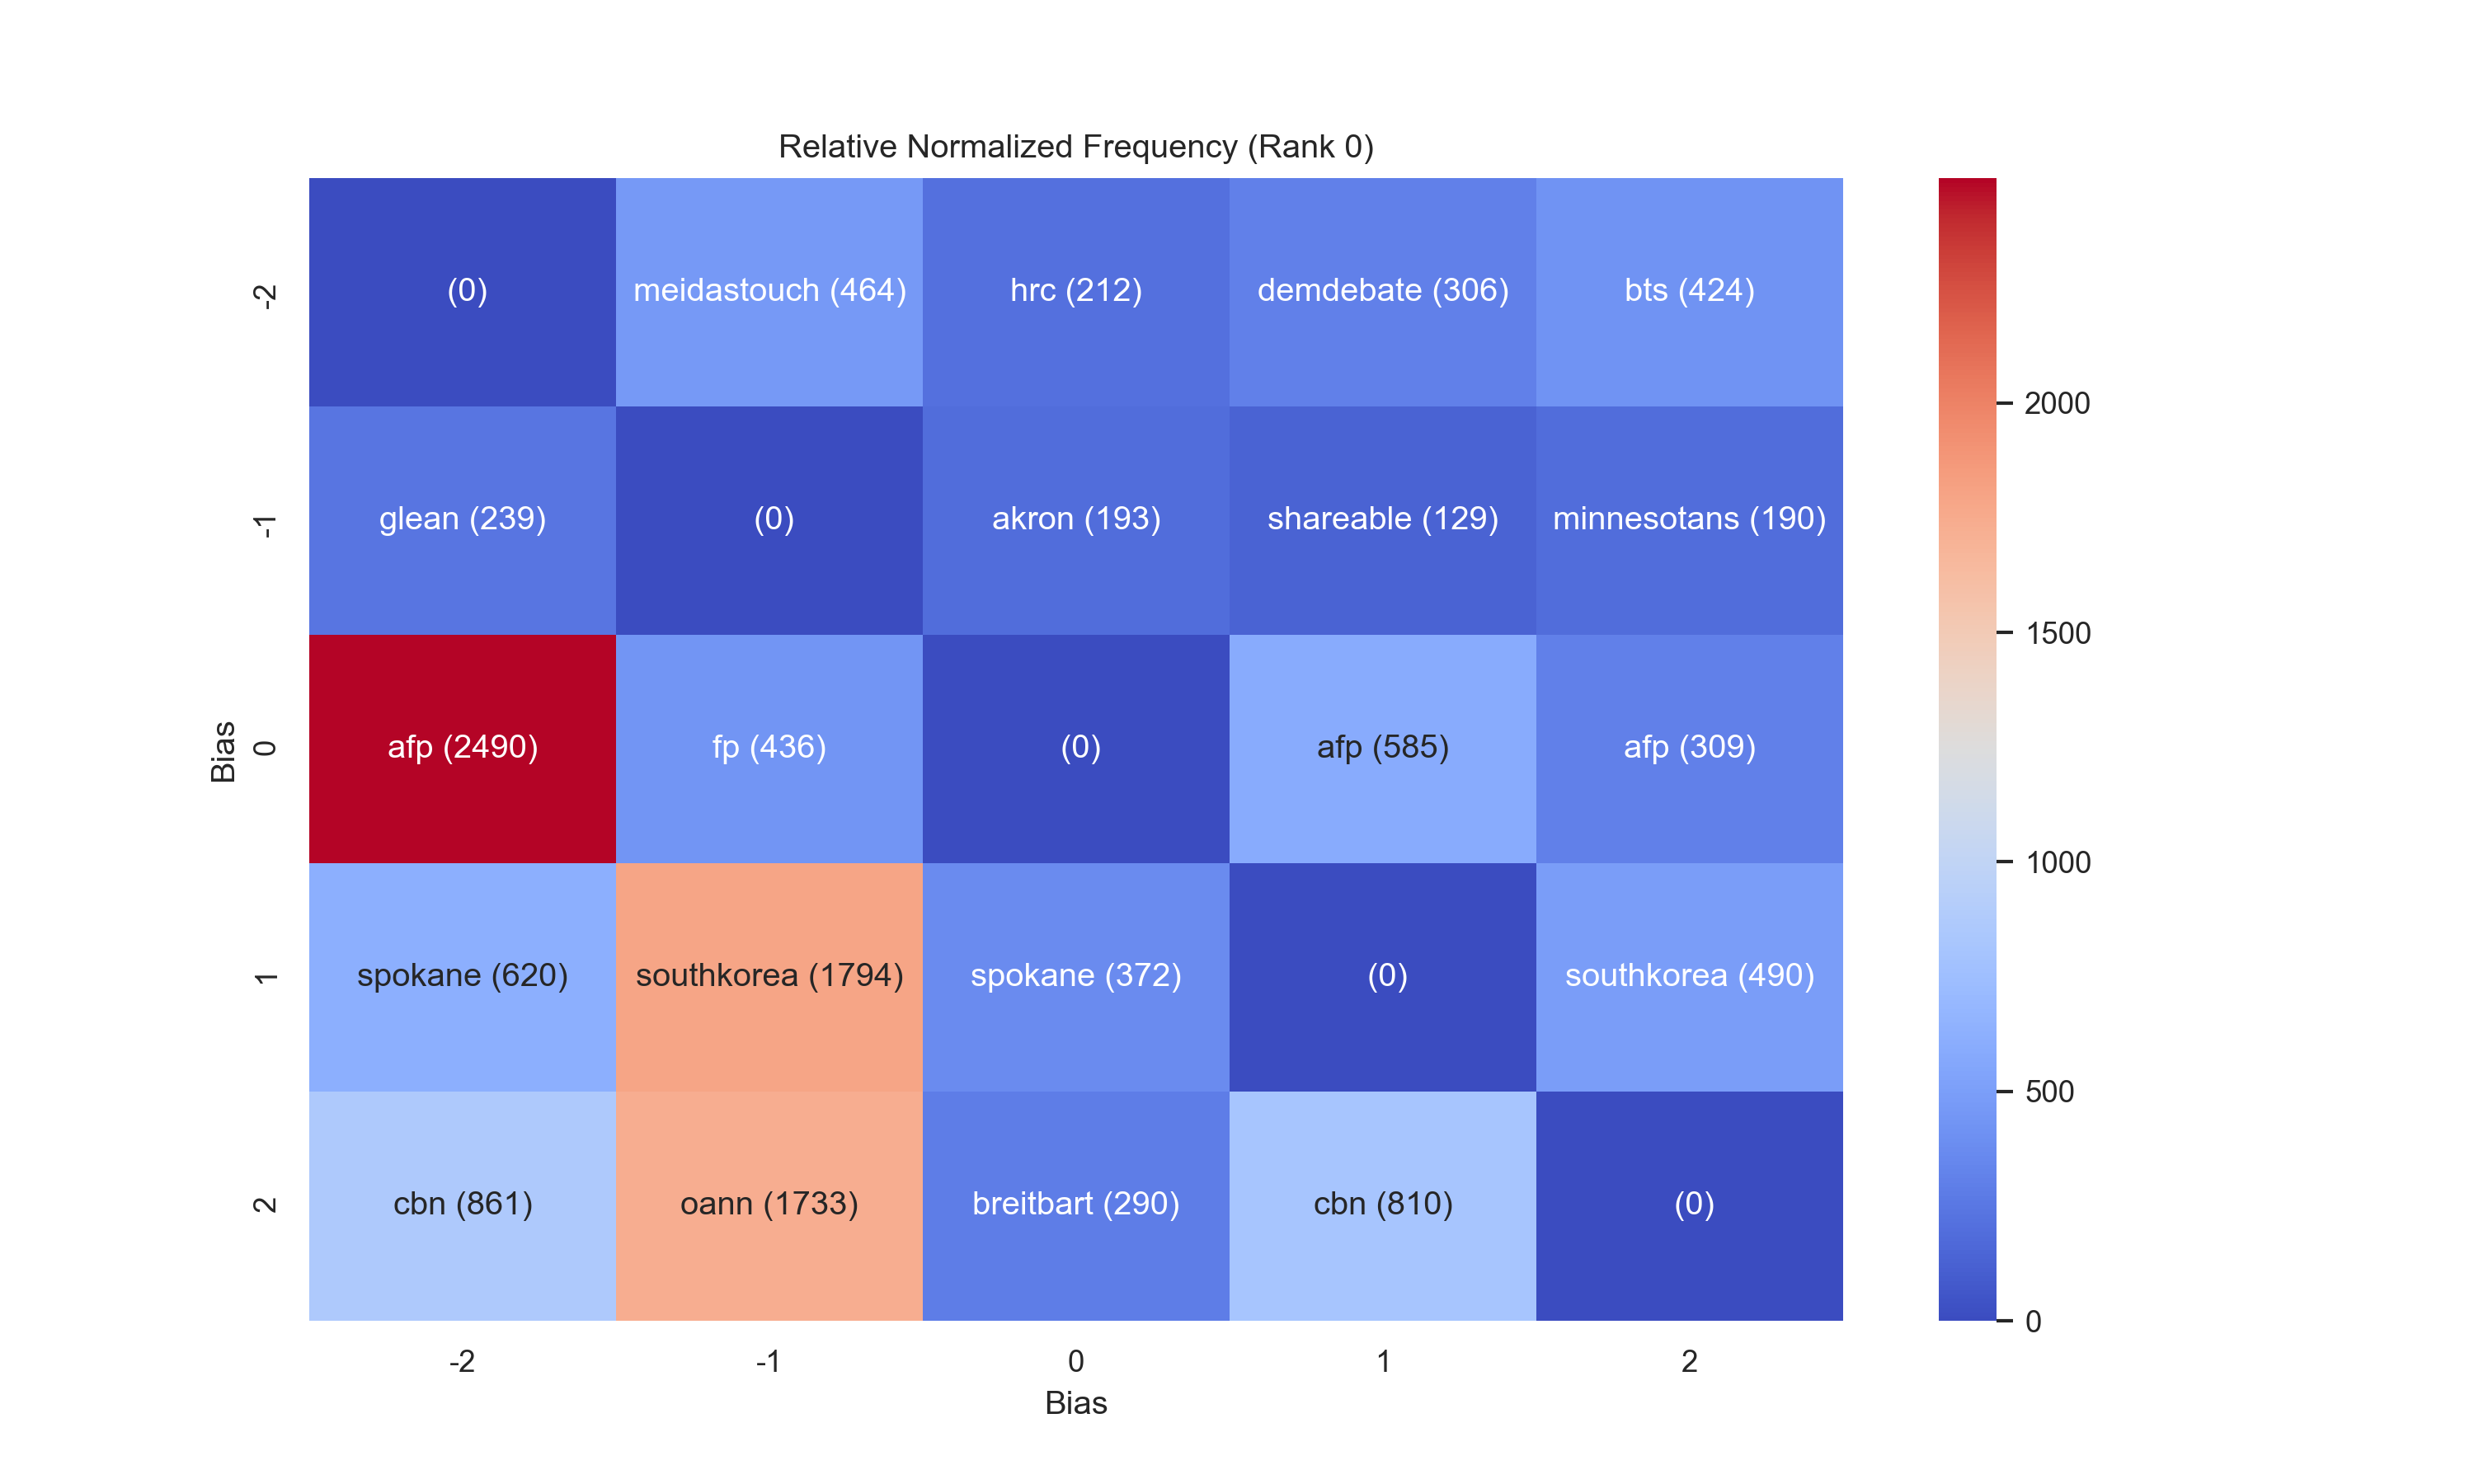
\includegraphics[width=0.6\textwidth]{figs/top_ten_rnf/rnf_w_rank_0.png}
\end{figure}
\end{center}

\subsubsection{Rank 1}
\begin{center}

\CatchFileDef{\TTRNFTable}{figs/top_ten_rnf/table_rnf_w_rank_1.latex.txt}

\resizebox{\columnwidth}{!}
{
\TTRNFTable
}
\begin{figure}[h!]
  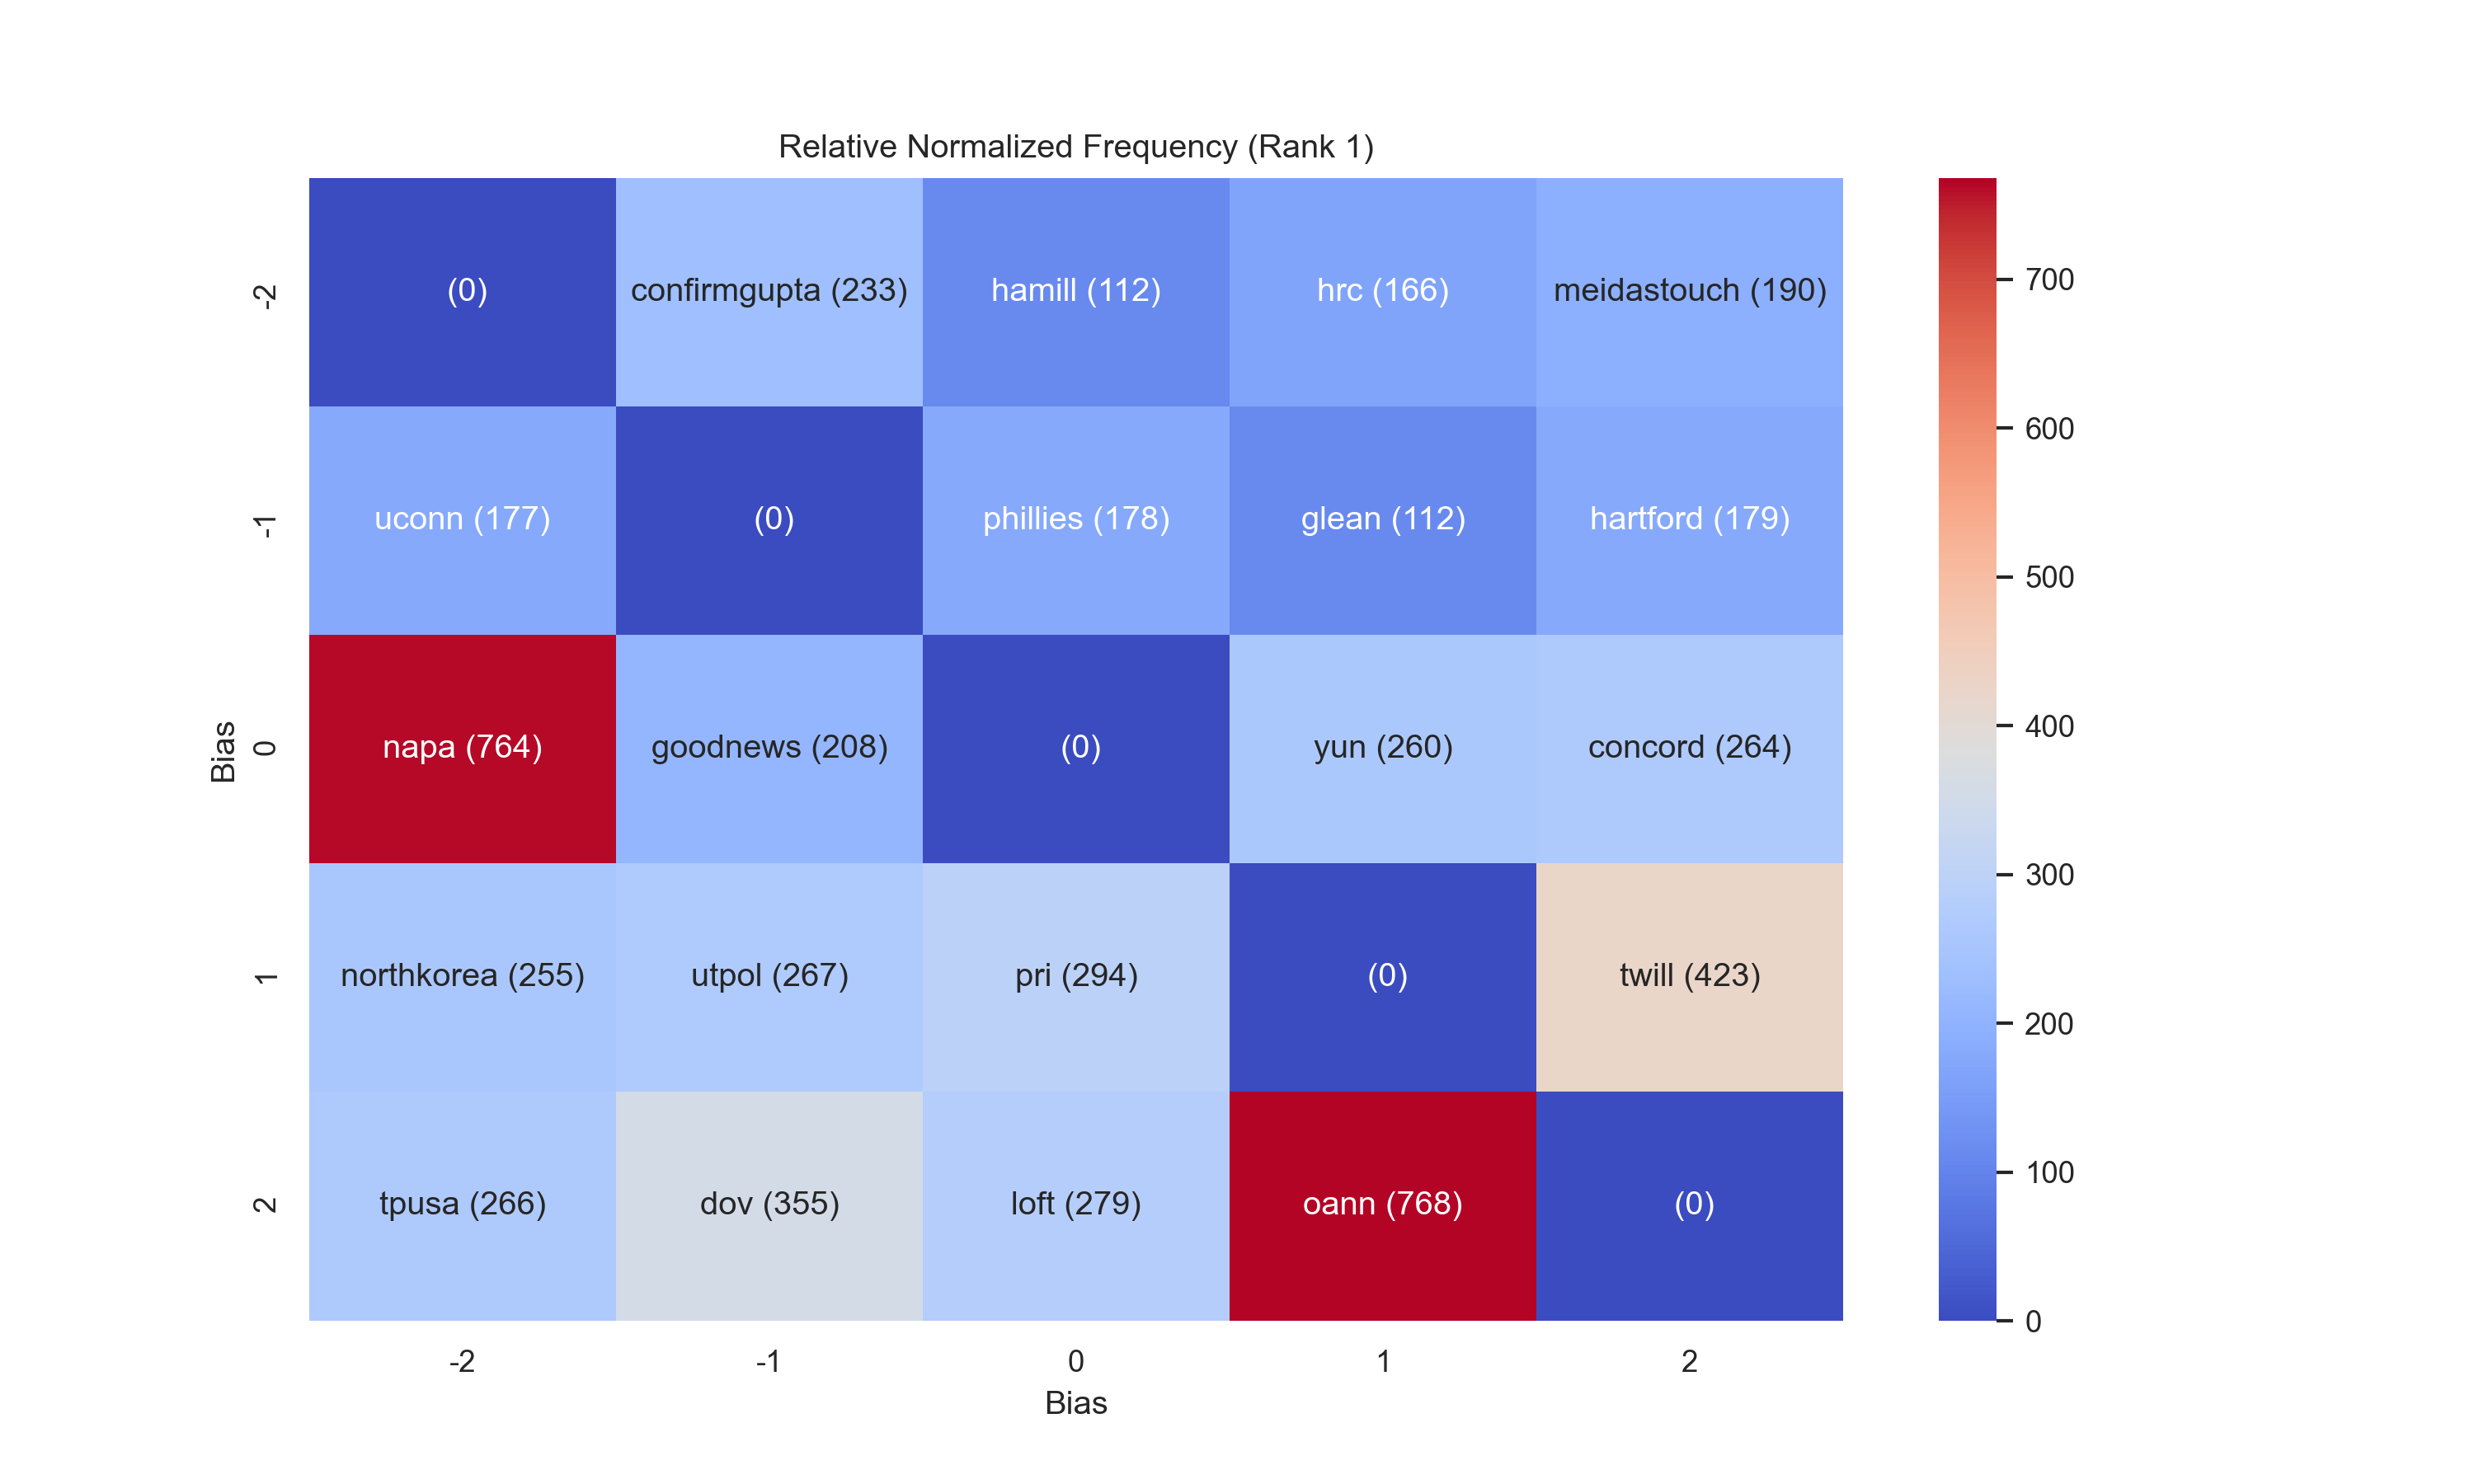
\includegraphics[width=0.6\textwidth]{figs/top_ten_rnf/rnf_w_rank_1.png}
\end{figure}
\end{center}

\pagebreak

\subsubsection{Rank 2}
\begin{center}

\CatchFileDef{\TTRNFTable}{figs/top_ten_rnf/table_rnf_w_rank_2.latex.txt}

\resizebox{\columnwidth}{!}
{
\TTRNFTable
}
\begin{figure}[h!]
  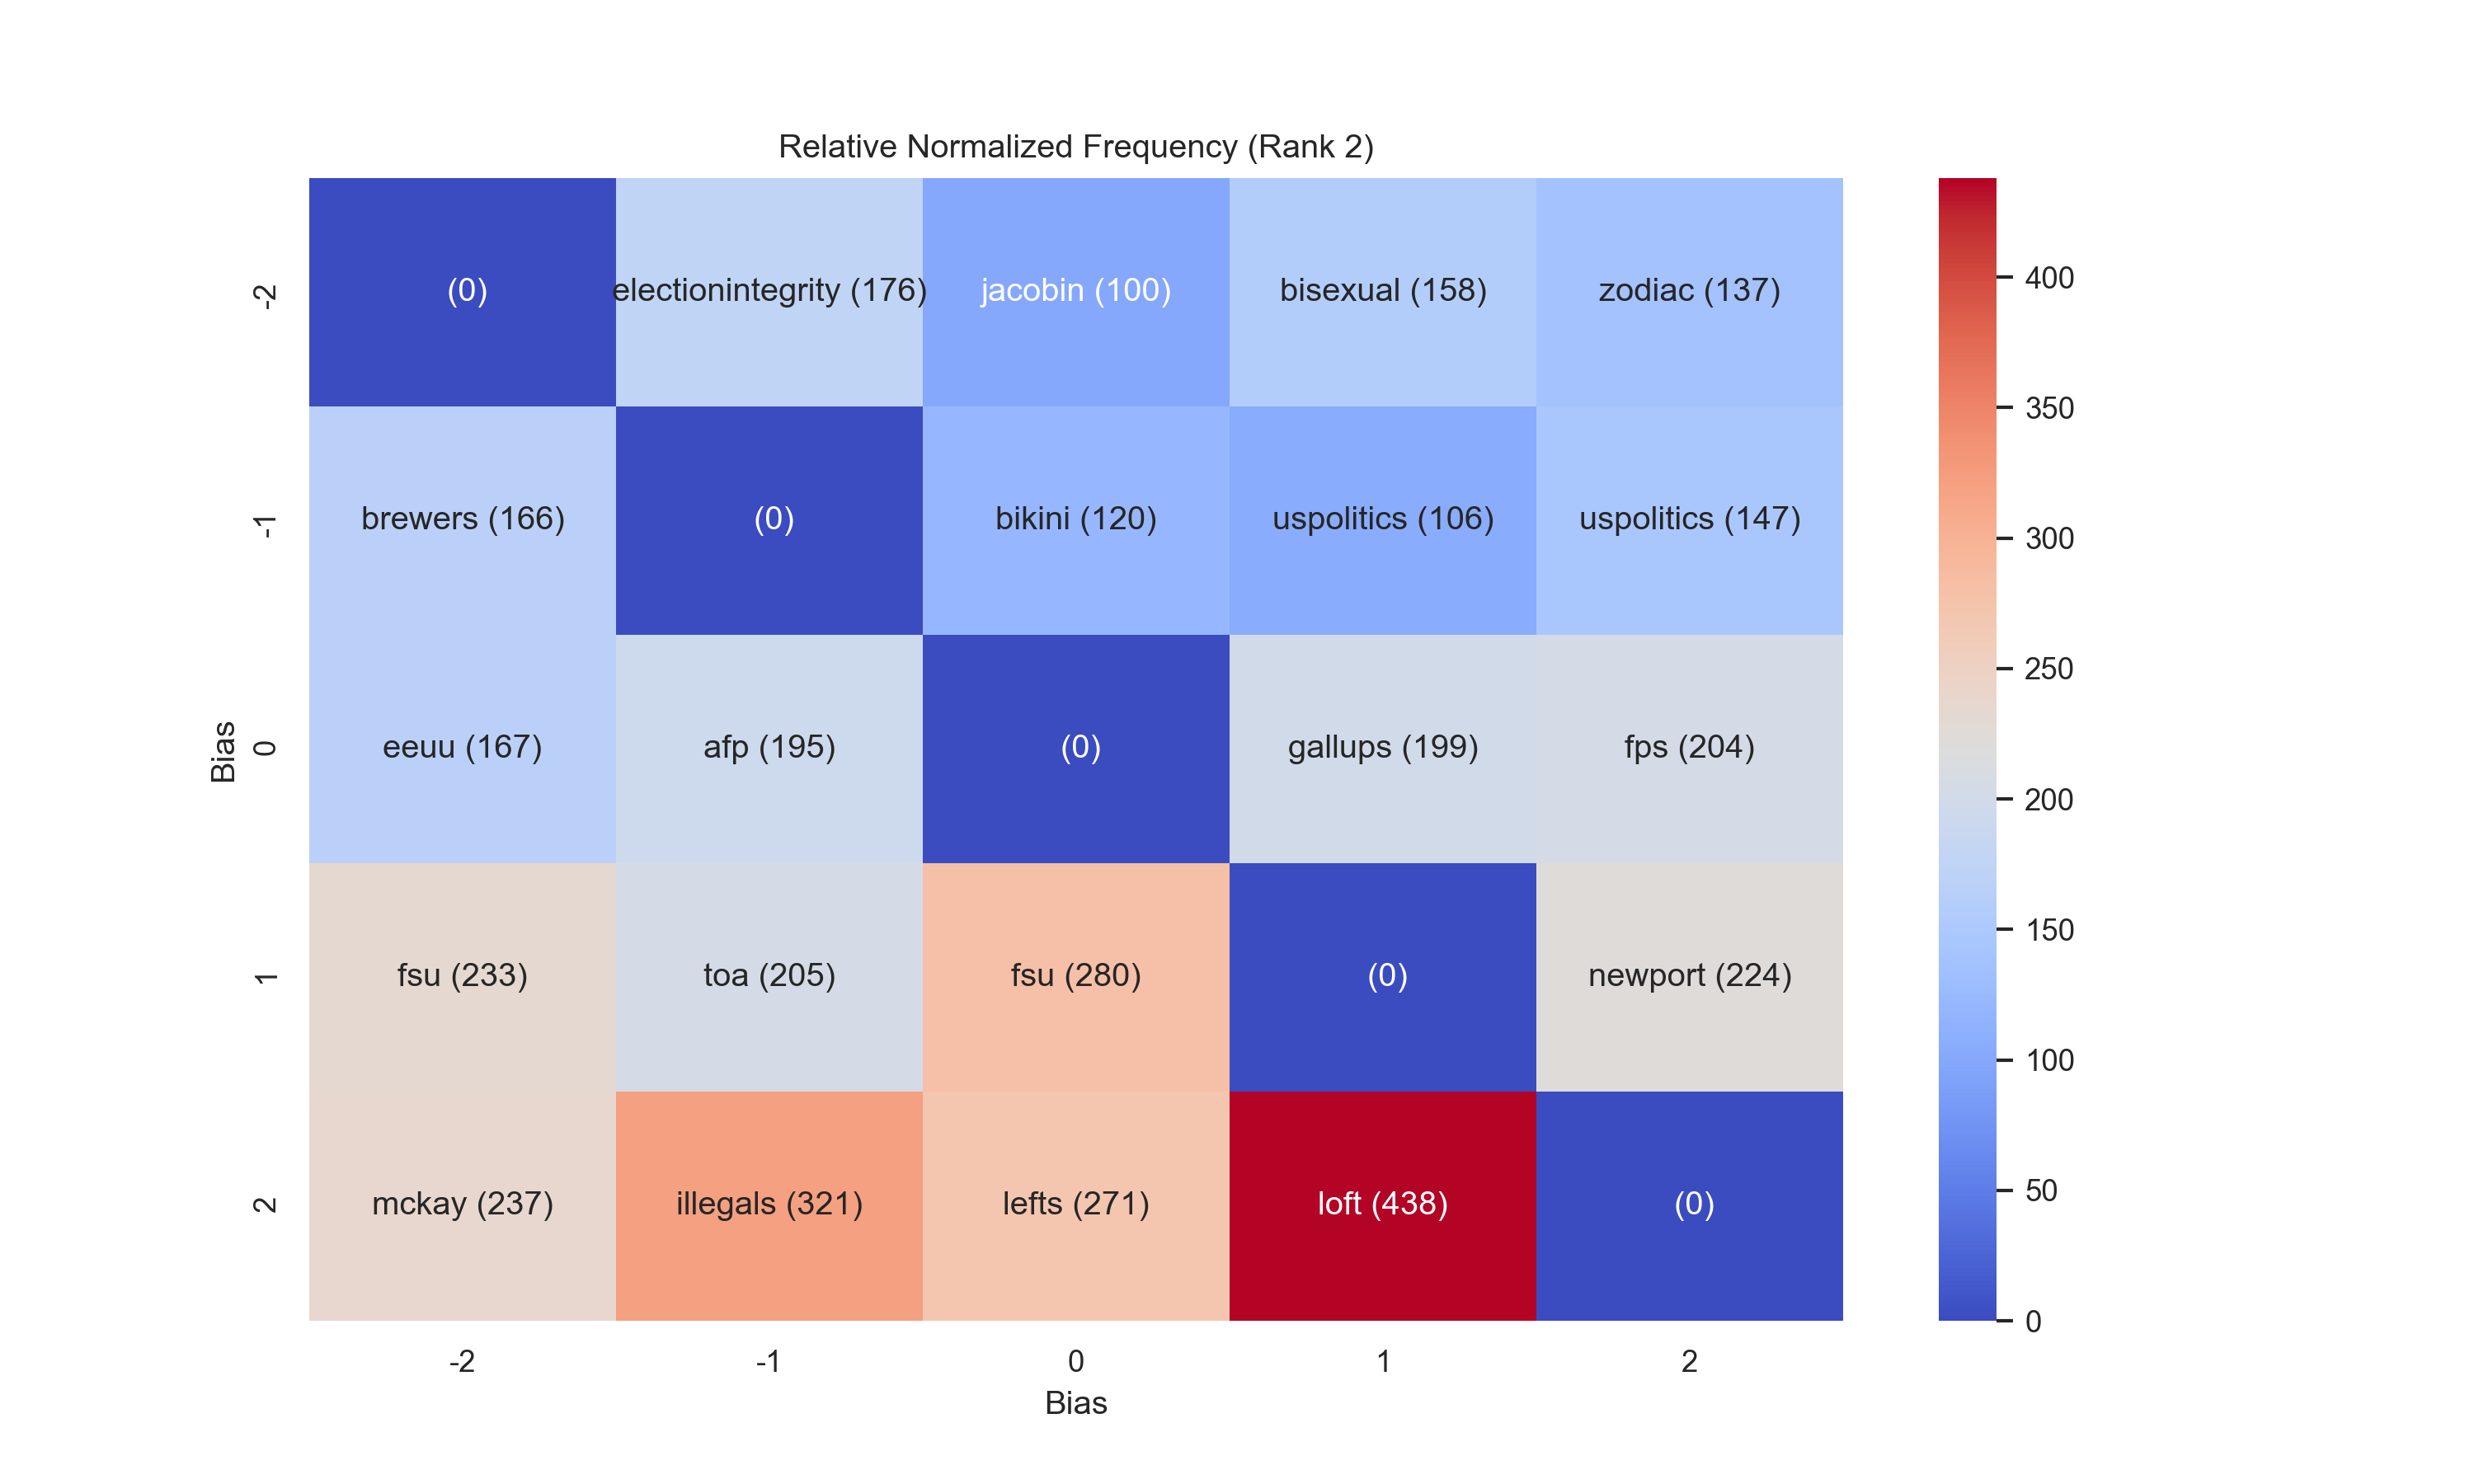
\includegraphics[width=0.6\textwidth]{figs/top_ten_rnf/rnf_w_rank_2.png}
\end{figure}
\end{center}

\subsubsection{Rank 3}
\begin{center}

\CatchFileDef{\TTRNFTable}{figs/top_ten_rnf/table_rnf_w_rank_3.latex.txt}

\resizebox{\columnwidth}{!}
{
\TTRNFTable
}
\begin{figure}[h!]
  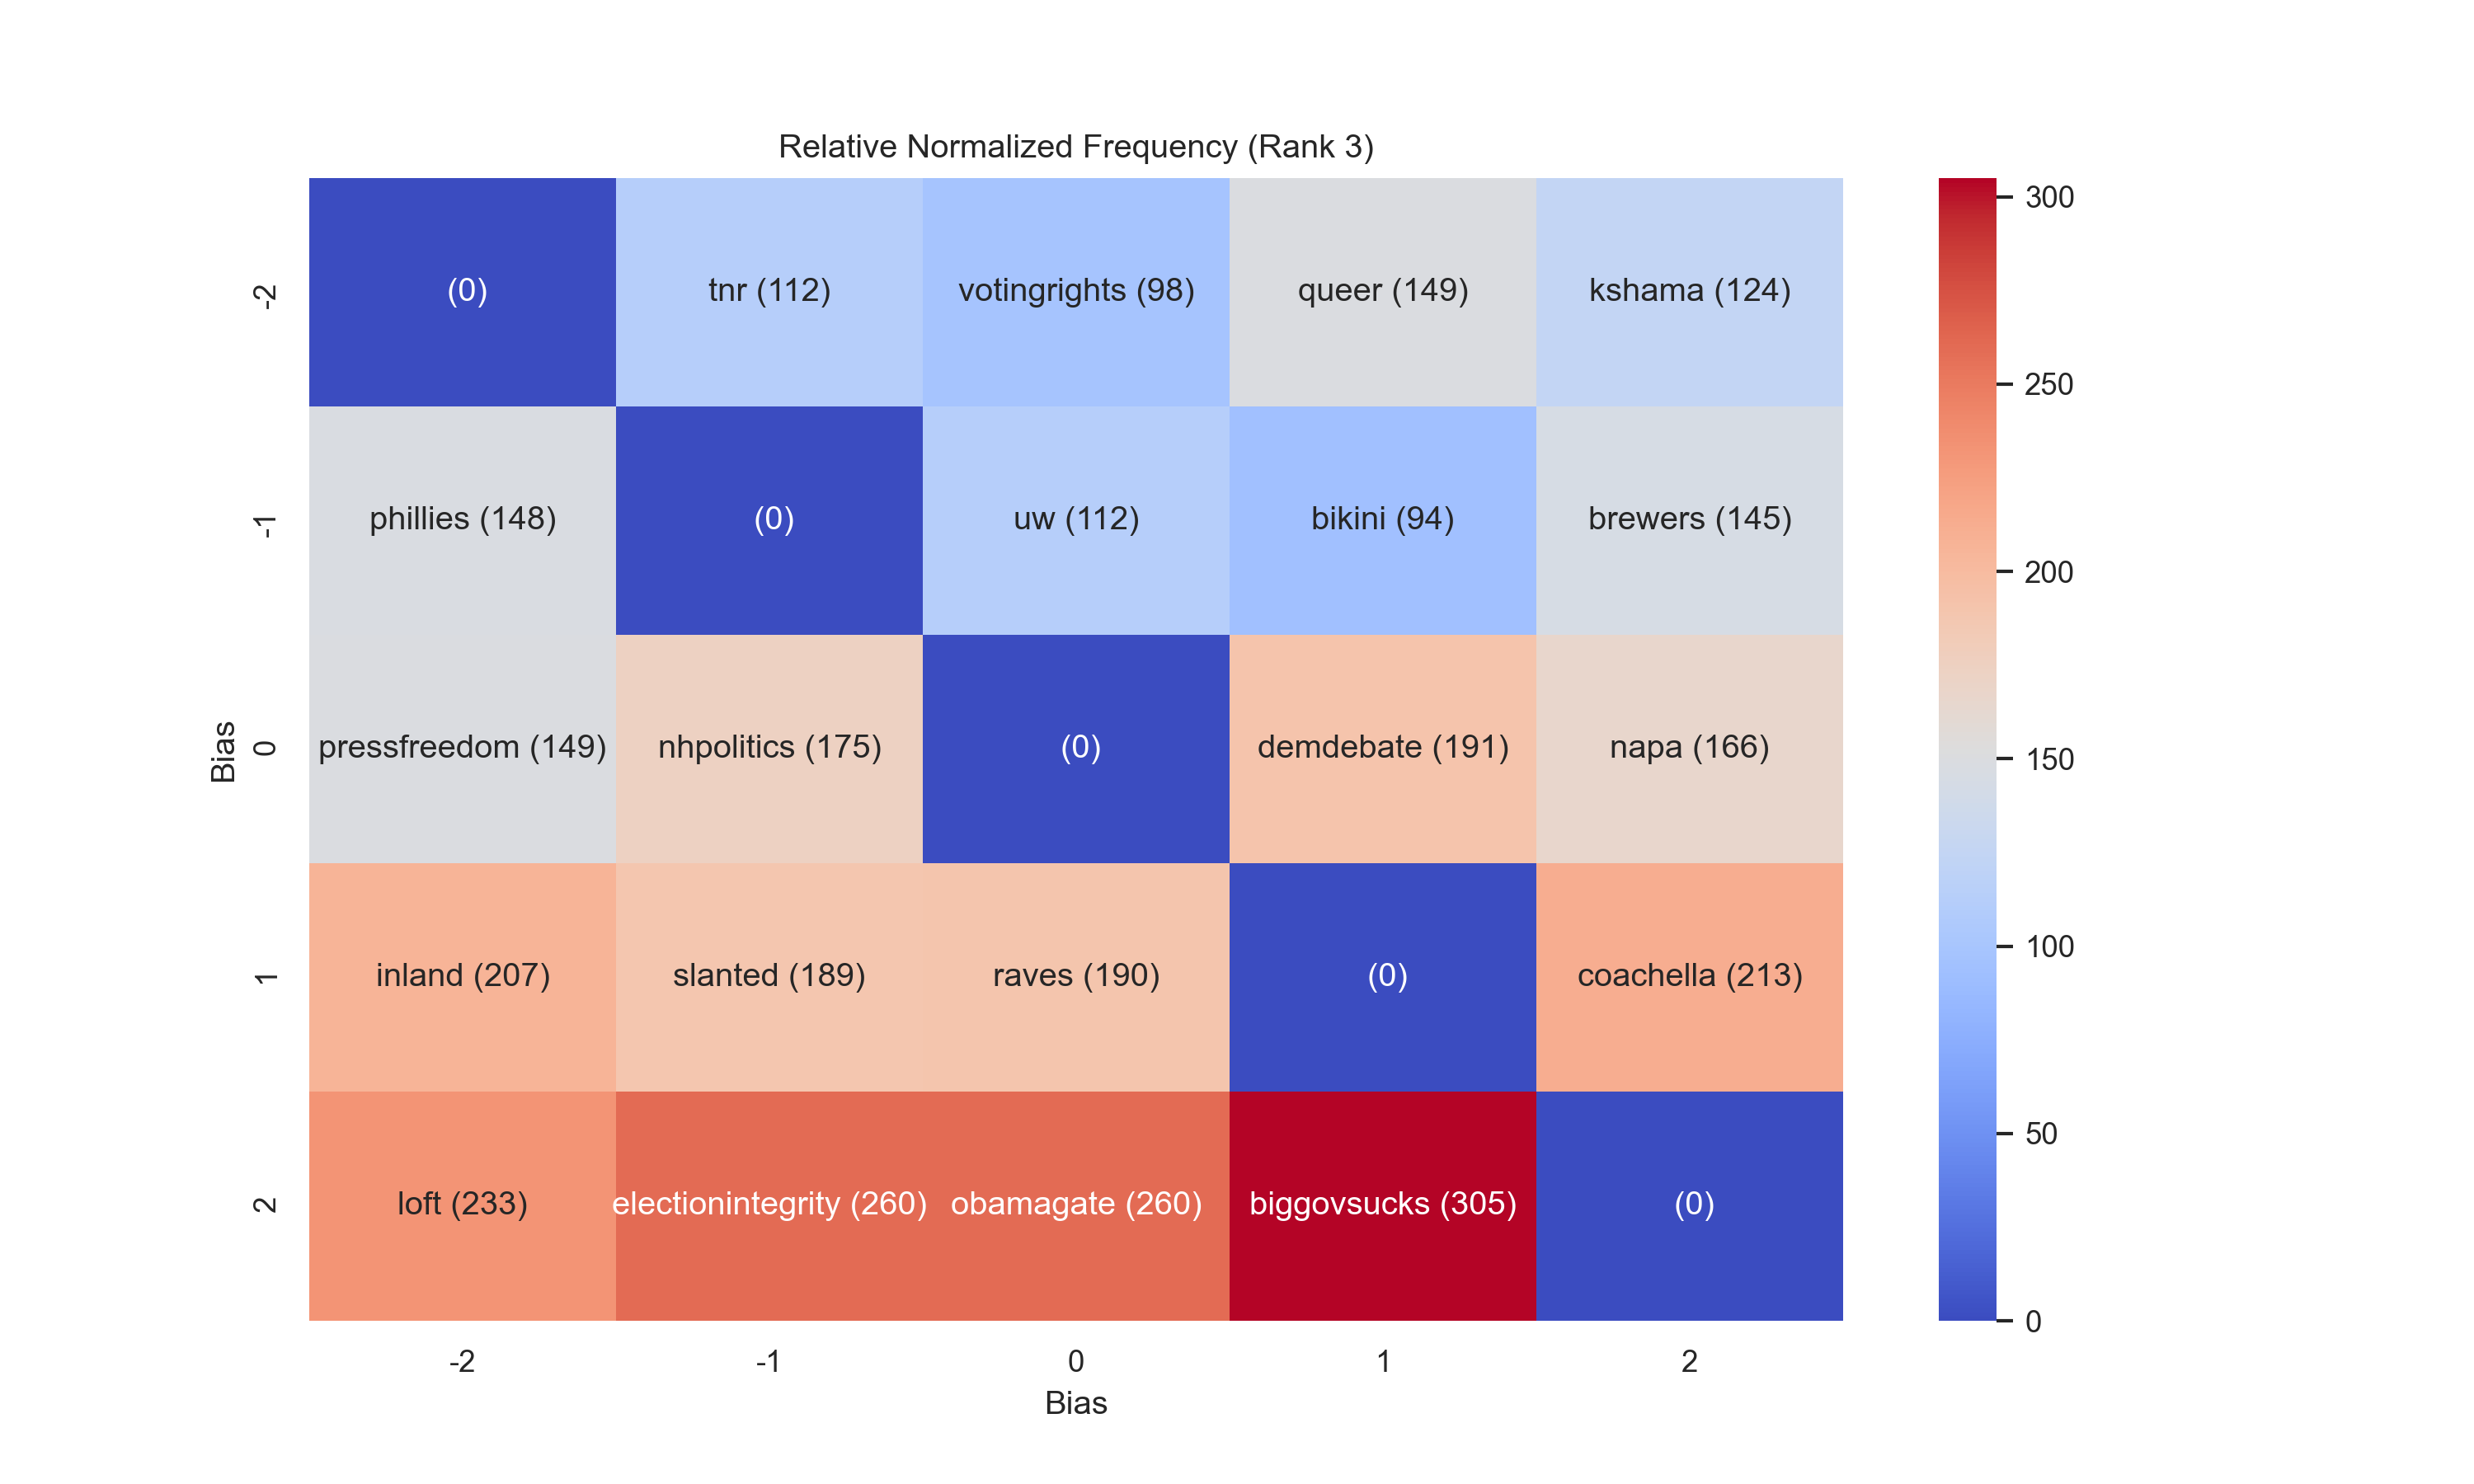
\includegraphics[width=0.6\textwidth]{figs/top_ten_rnf/rnf_w_rank_3.png}
\end{figure}
\end{center}

\pagebreak

\subsubsection{Rank 4}
\begin{center}

\CatchFileDef{\TTRNFTable}{figs/top_ten_rnf/table_rnf_w_rank_4.latex.txt}

\resizebox{\columnwidth}{!}
{
\TTRNFTable
}
\begin{figure}[h!]
  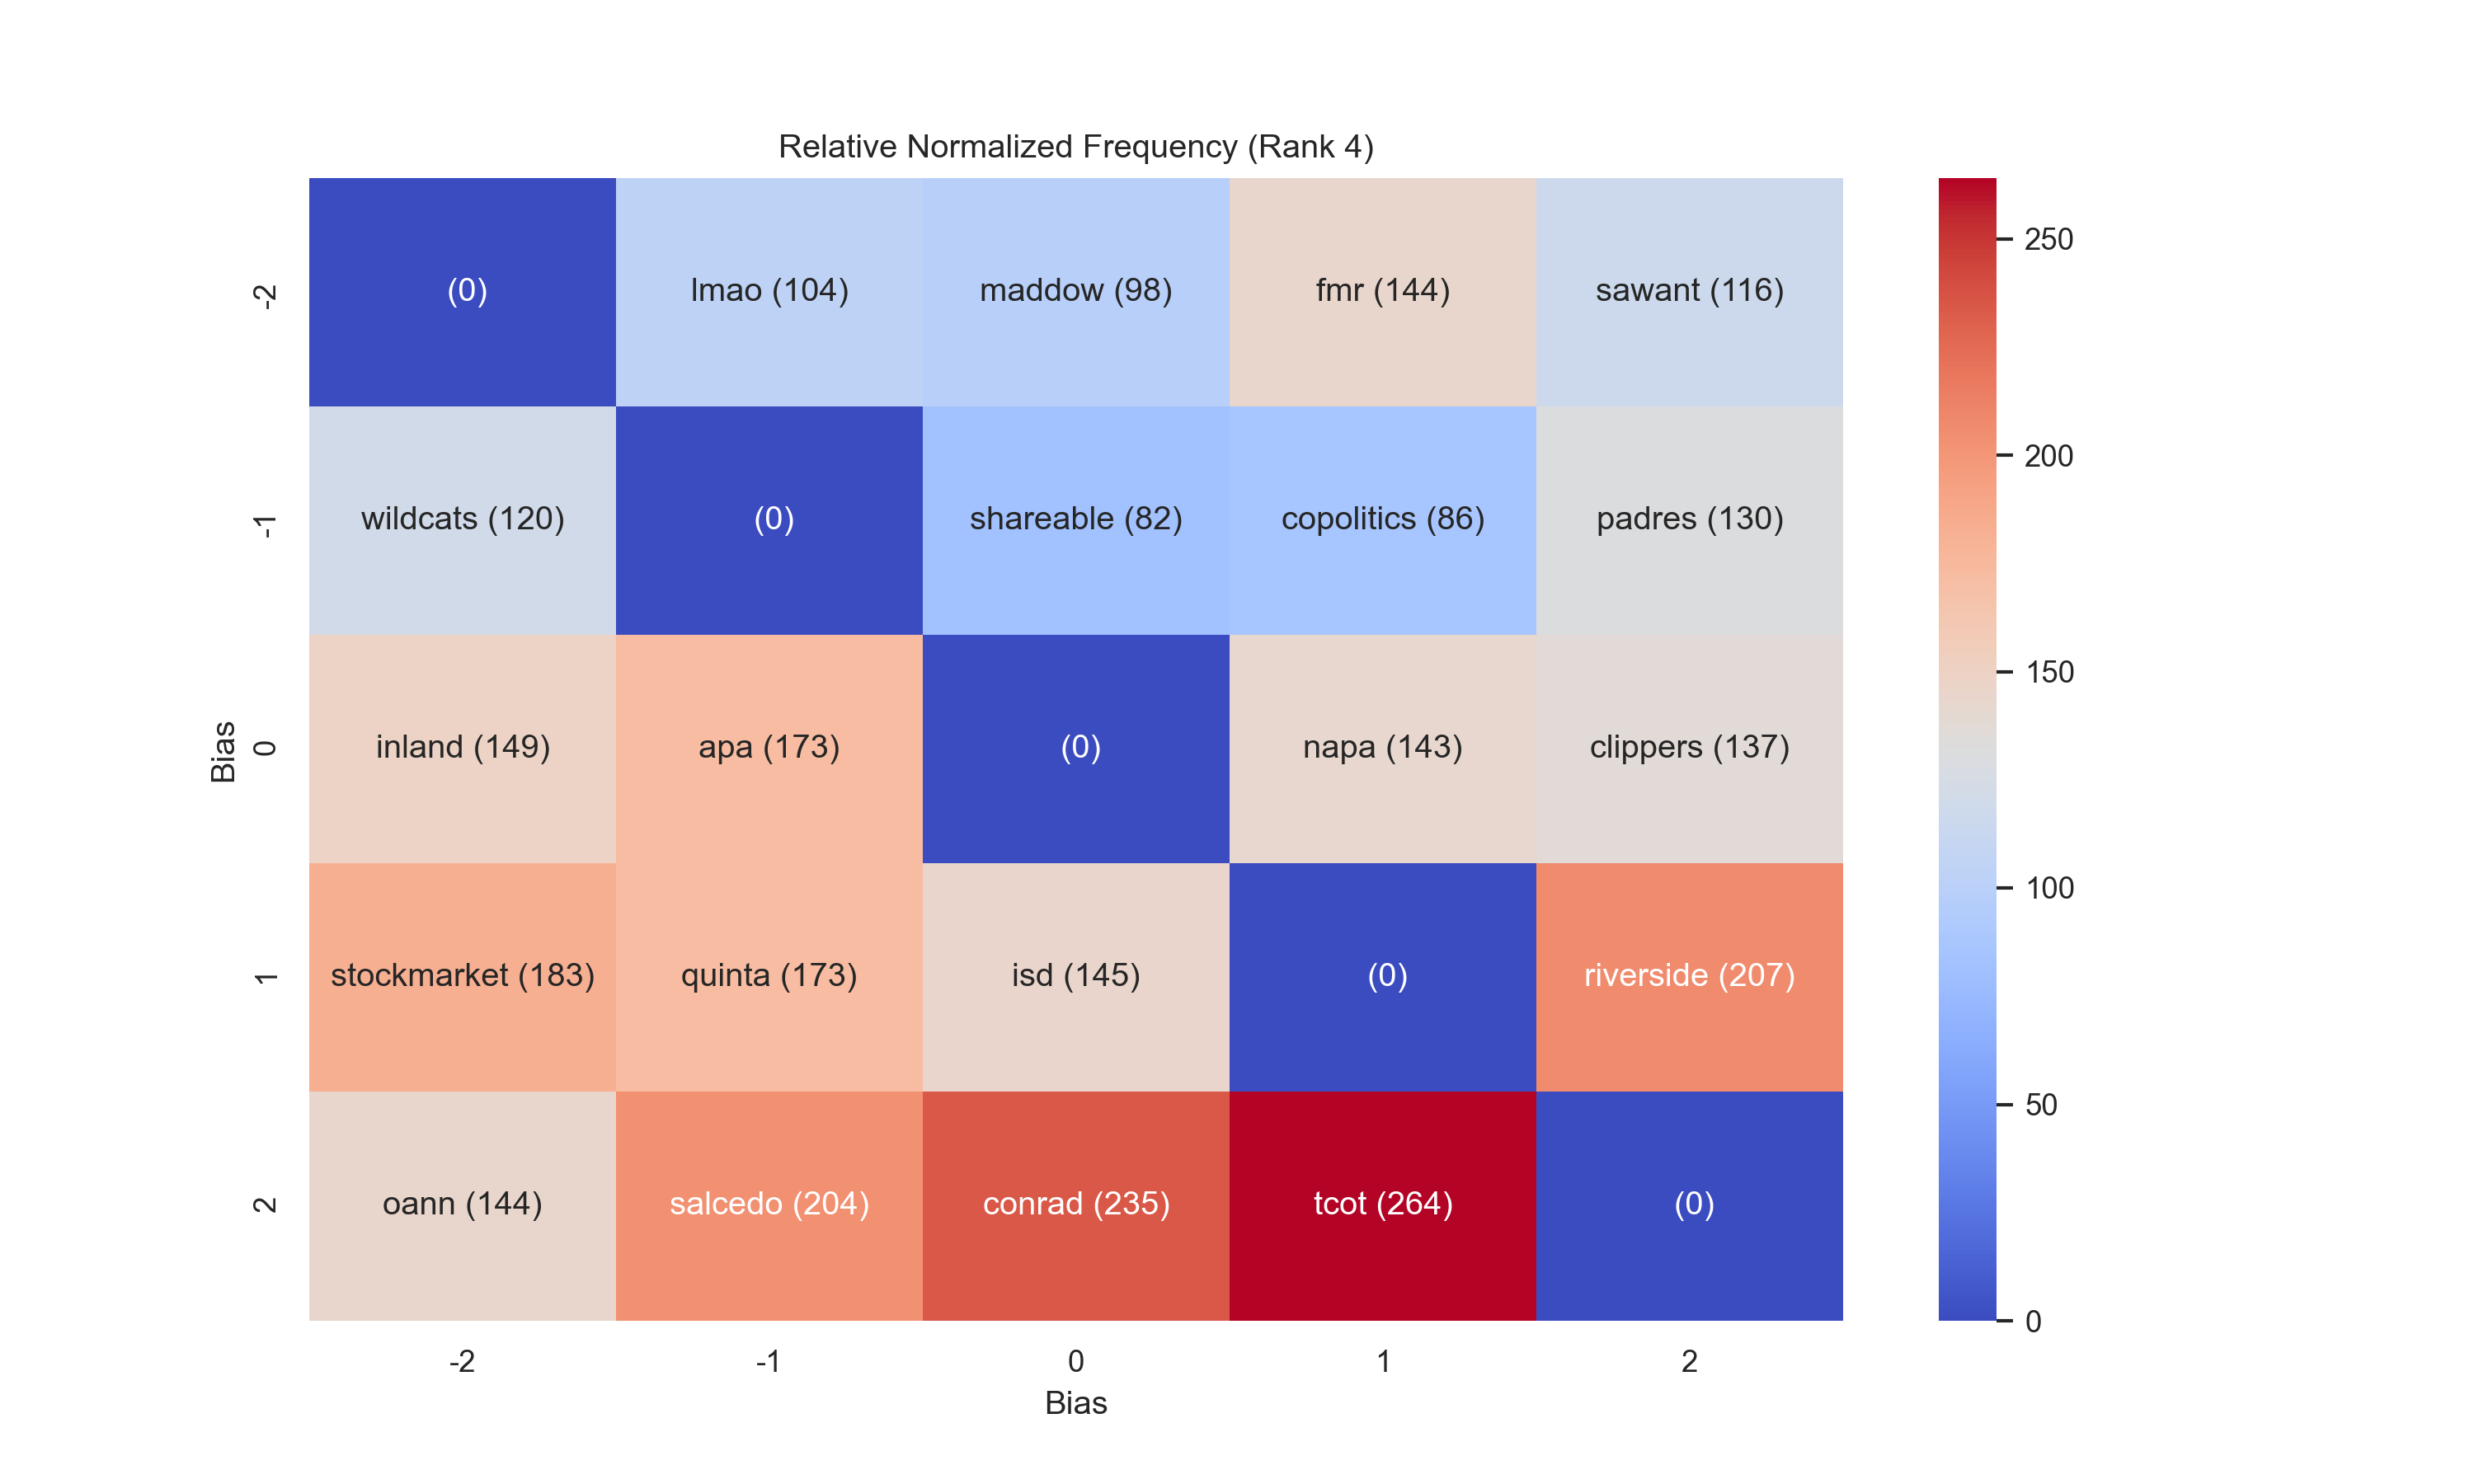
\includegraphics[width=0.6\textwidth]{figs/top_ten_rnf/rnf_w_rank_4.png}
\end{figure}
\end{center}

\subsubsection{Rank 5}
\begin{center}

\CatchFileDef{\TTRNFTable}{figs/top_ten_rnf/table_rnf_w_rank_5.latex.txt}

\resizebox{\columnwidth}{!}
{
\TTRNFTable
}
\begin{figure}[h!]
  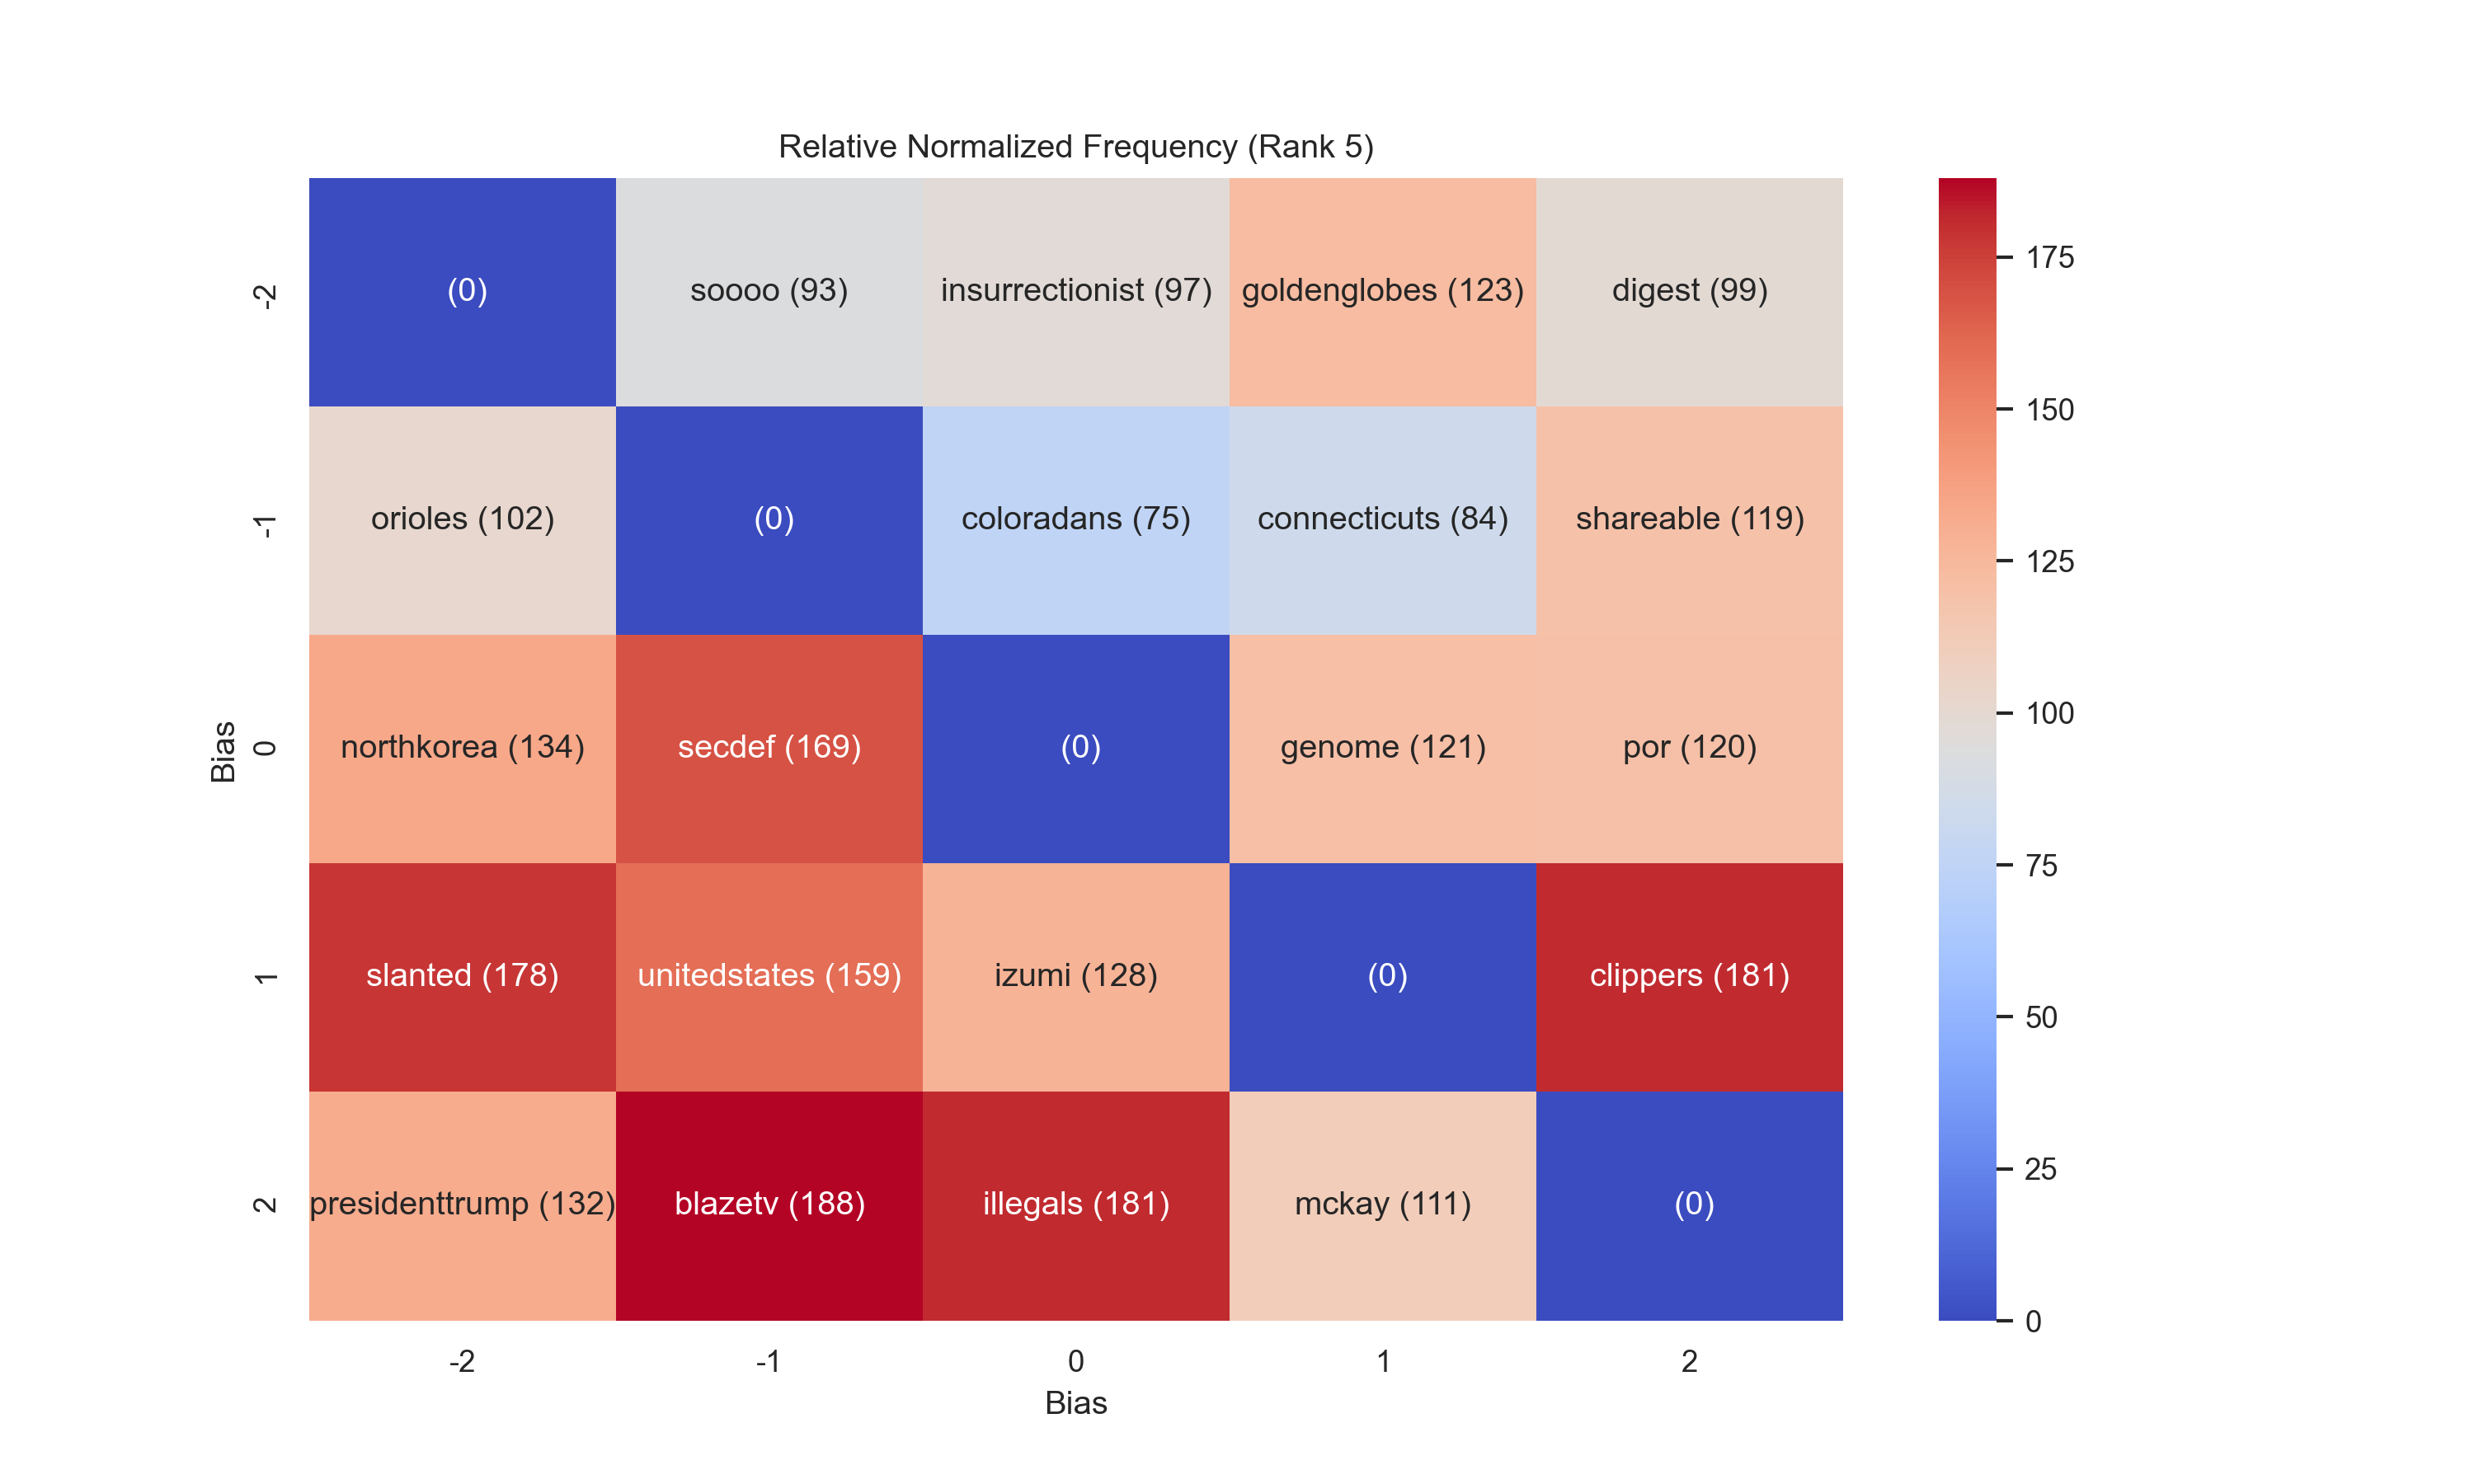
\includegraphics[width=0.6\textwidth]{figs/top_ten_rnf/rnf_w_rank_5.png}
\end{figure}
\end{center}

\pagebreak

\subsubsection{Rank 6}
\begin{center}

\CatchFileDef{\TTRNFTable}{figs/top_ten_rnf/table_rnf_w_rank_6.latex.txt}

\resizebox{\columnwidth}{!}
{
\TTRNFTable
}
\begin{figure}[h!]
  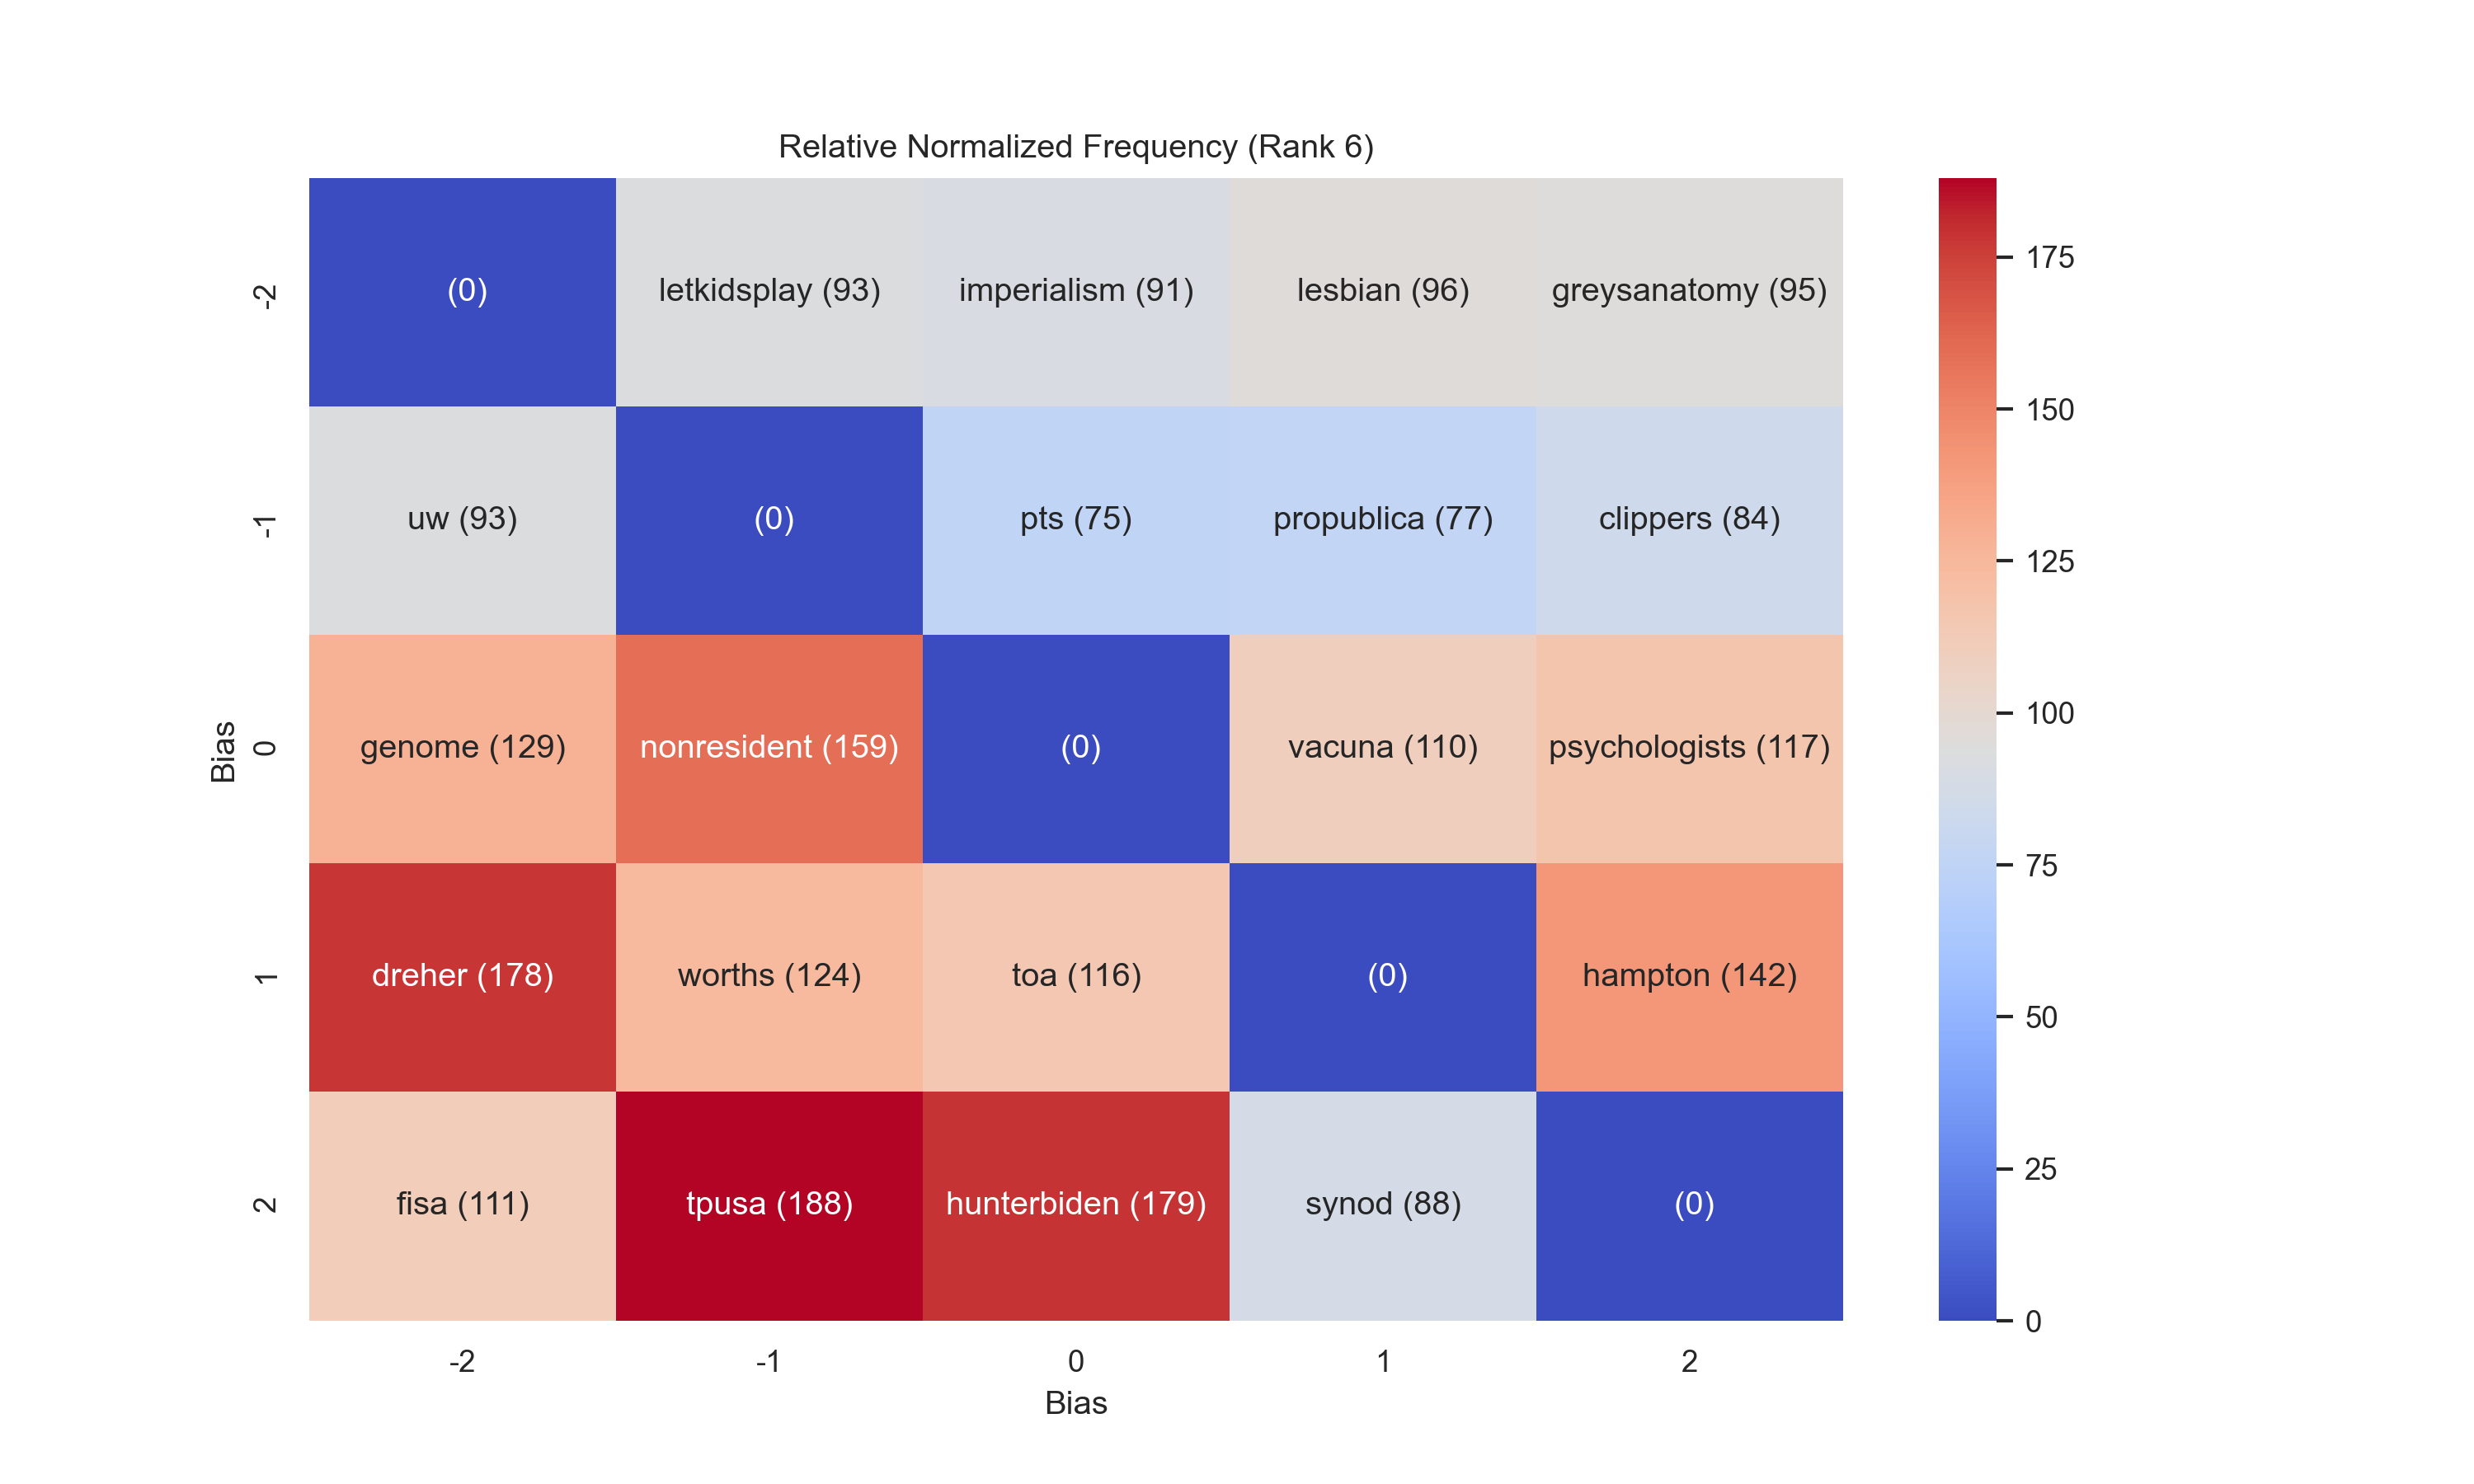
\includegraphics[width=0.6\textwidth]{figs/top_ten_rnf/rnf_w_rank_6.png}
\end{figure}
\end{center}

\subsubsection{Rank 7}
\begin{center}

\CatchFileDef{\TTRNFTable}{figs/top_ten_rnf/table_rnf_w_rank_7.latex.txt}

\resizebox{\columnwidth}{!}
{
\TTRNFTable
}
\begin{figure}[h!]
  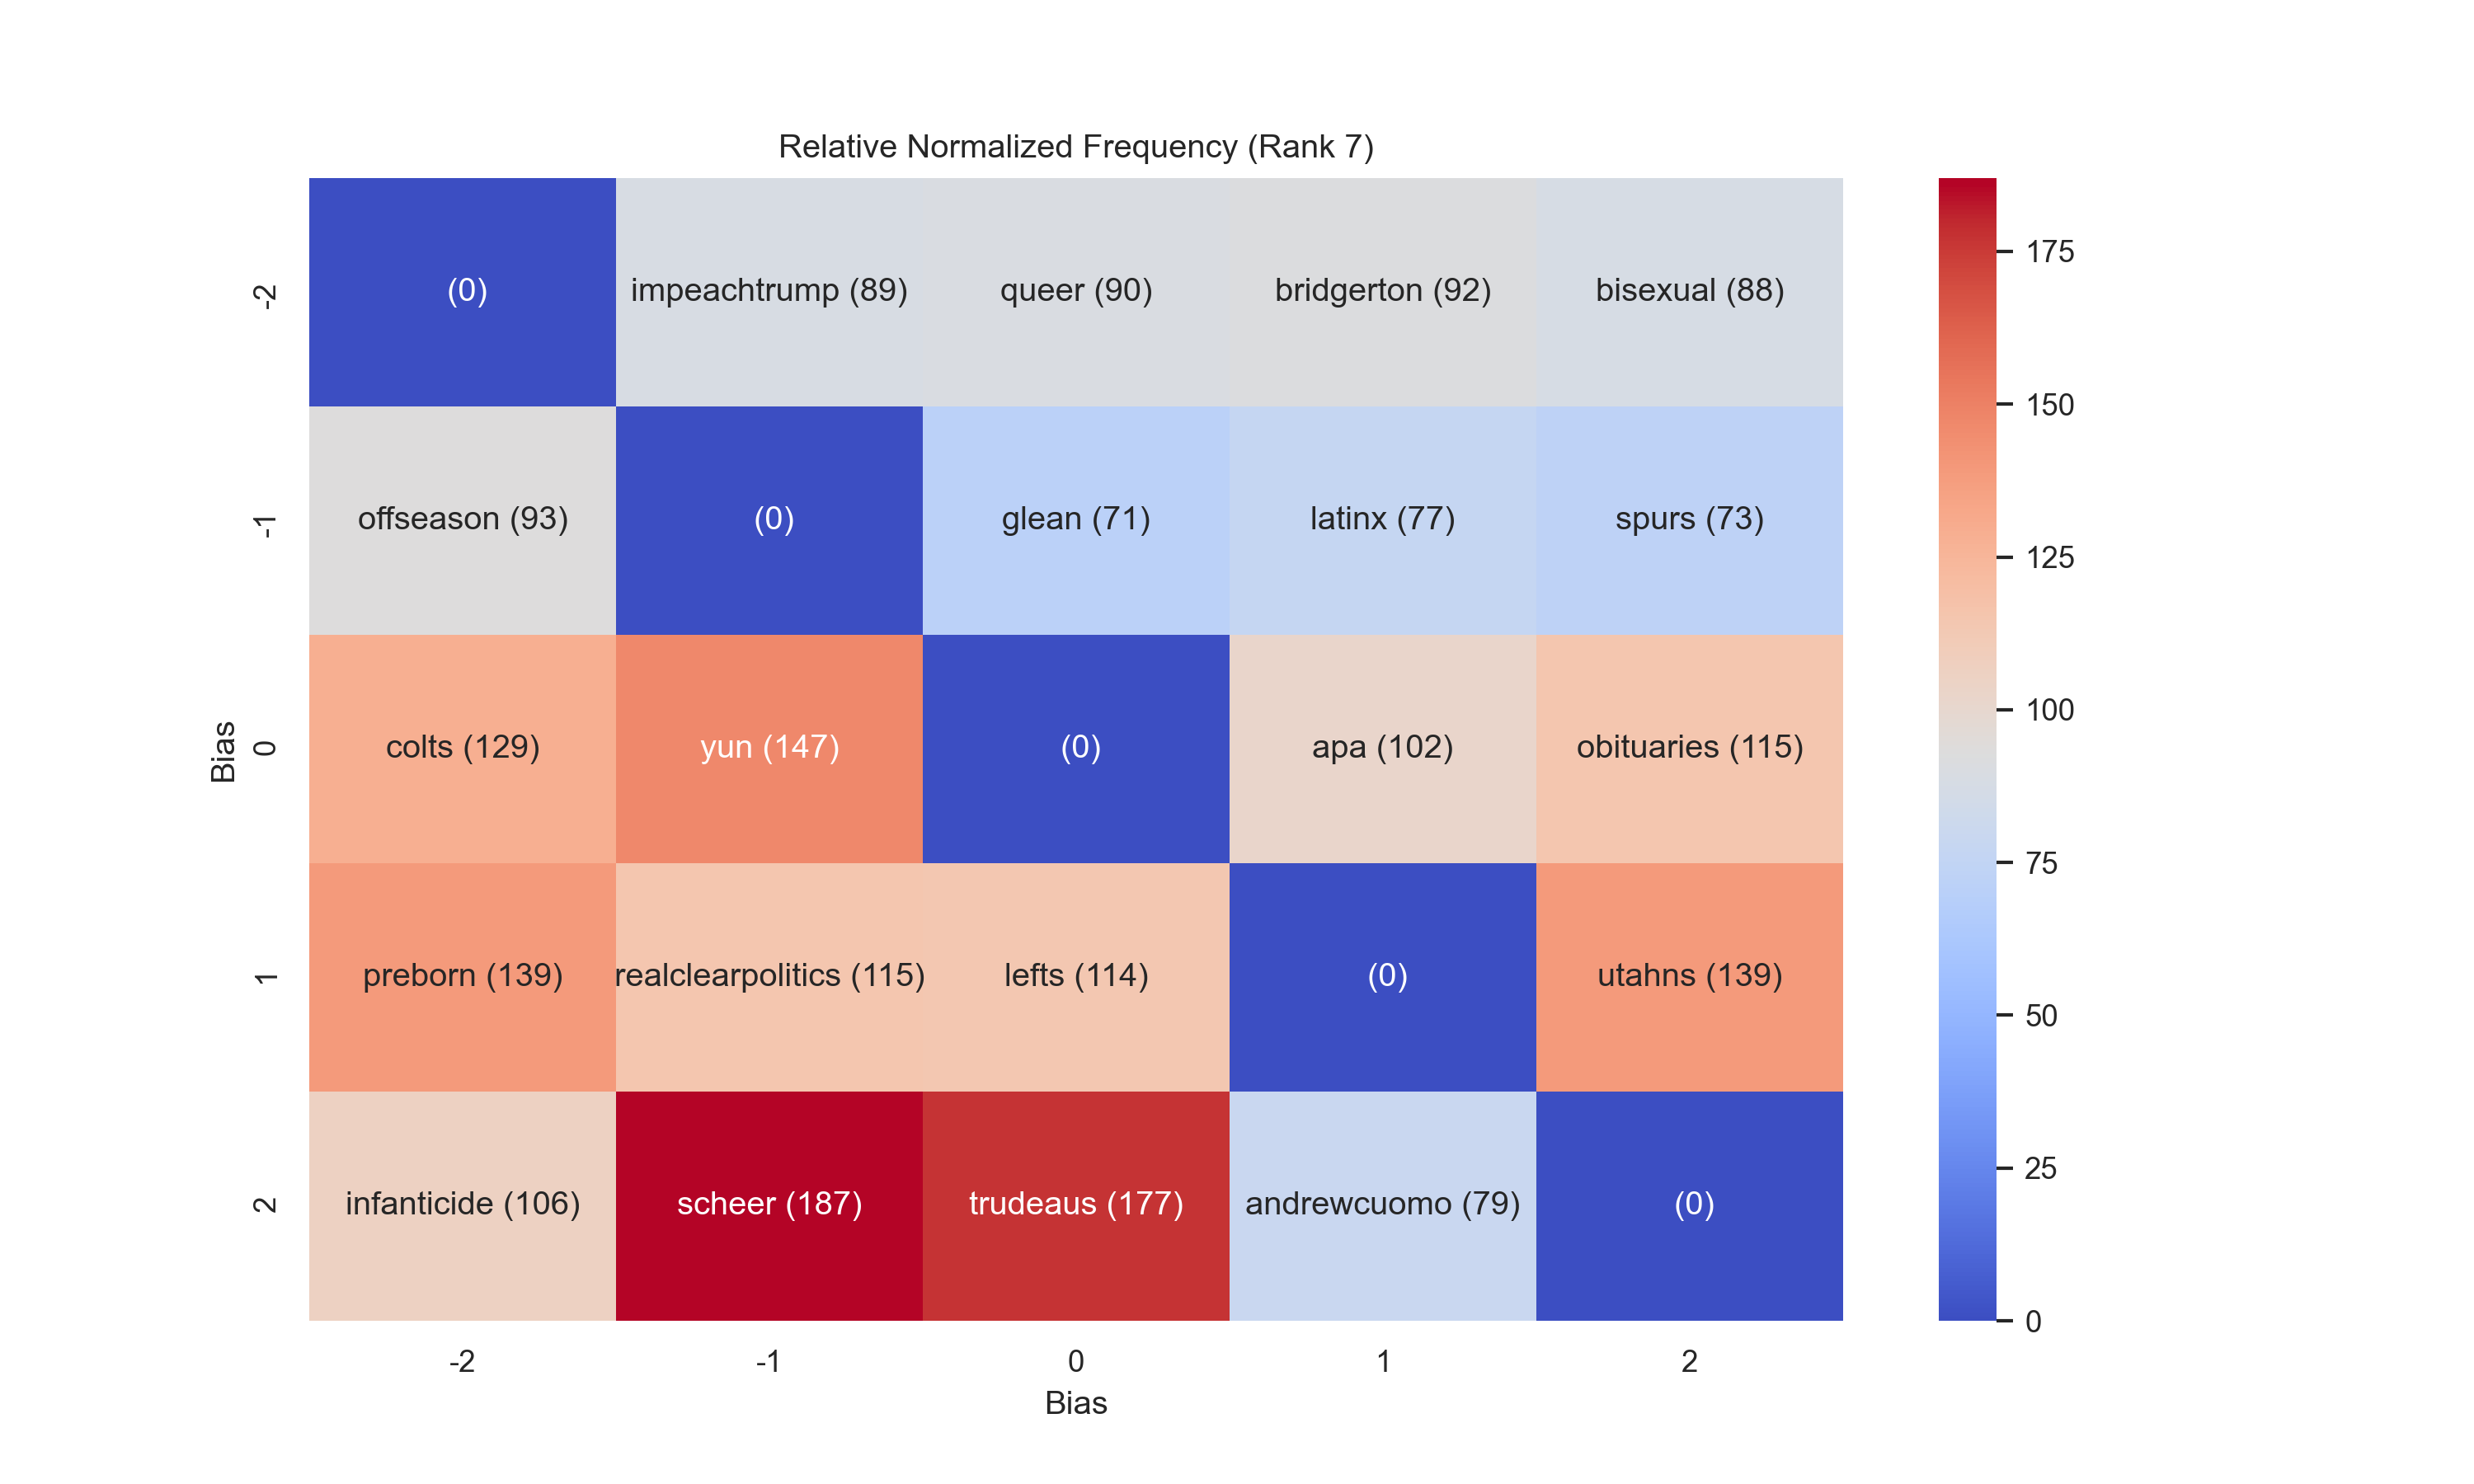
\includegraphics[width=0.6\textwidth]{figs/top_ten_rnf/rnf_w_rank_7.png}
\end{figure}
\end{center}

\pagebreak

\subsubsection{Rank 8}
\begin{center}

\CatchFileDef{\TTRNFTable}{figs/top_ten_rnf/table_rnf_w_rank_8.latex.txt}

\resizebox{\columnwidth}{!}
{
\TTRNFTable
}
\begin{figure}[h!]
  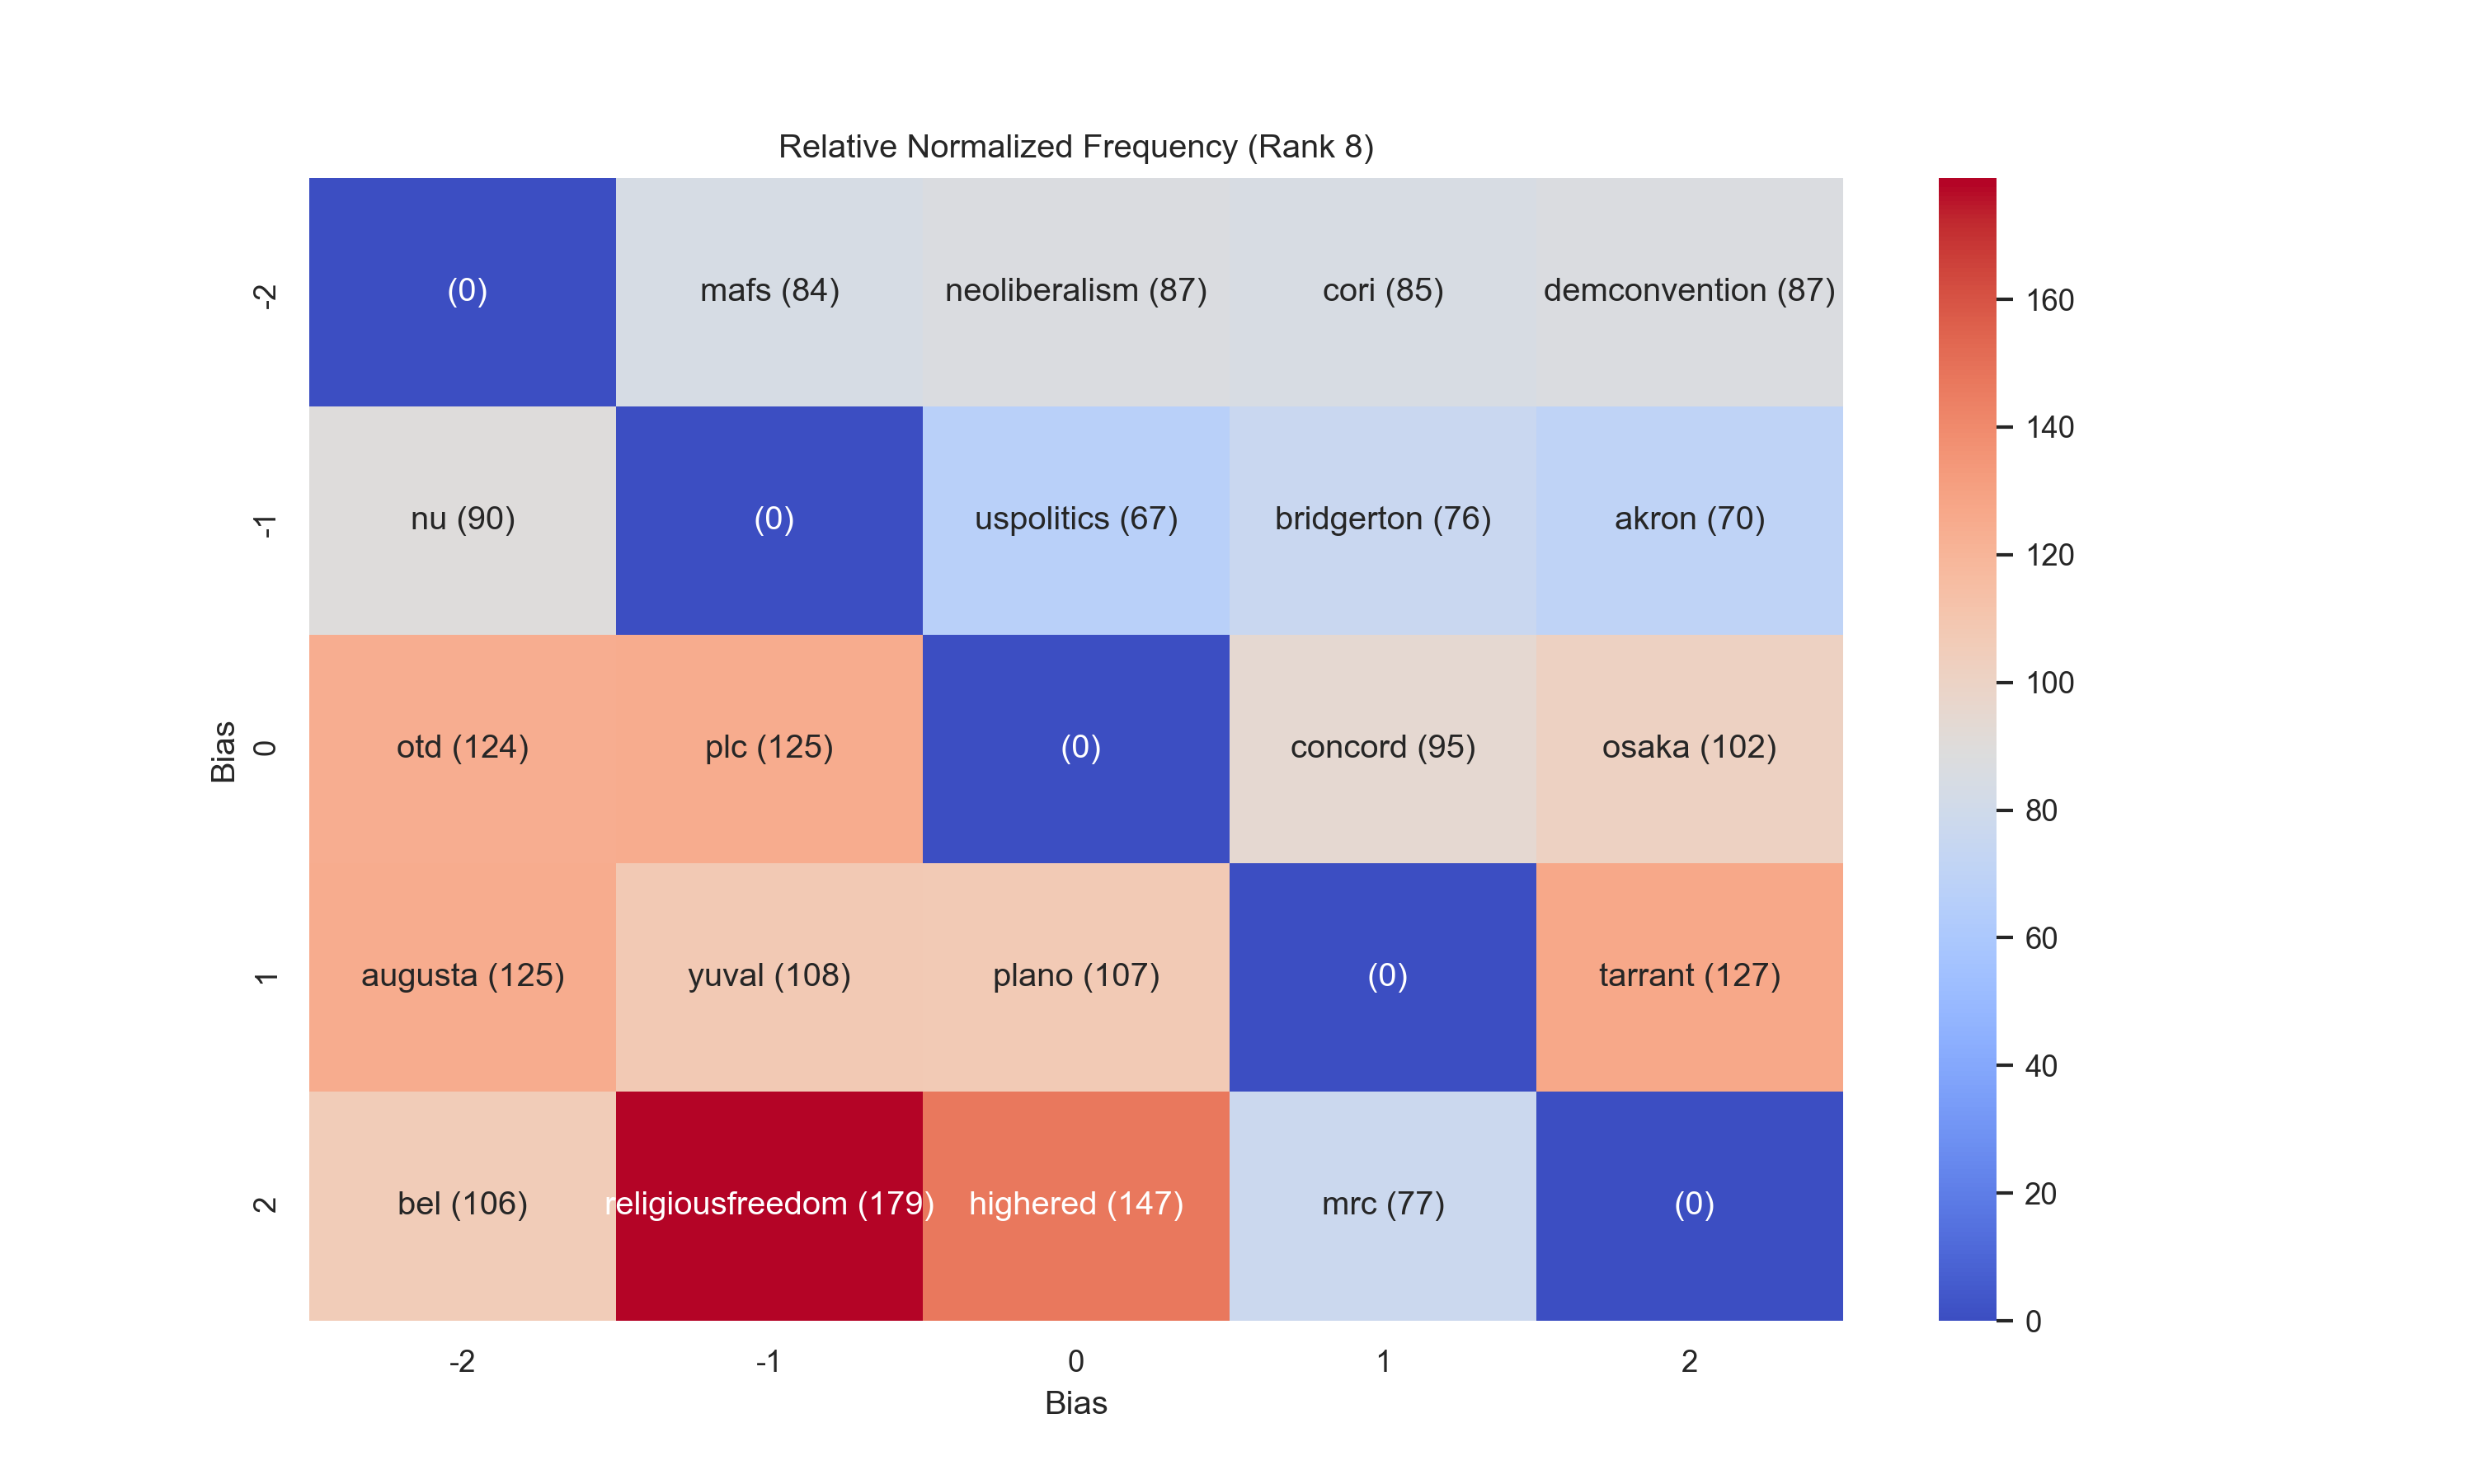
\includegraphics[width=0.6\textwidth]{figs/top_ten_rnf/rnf_w_rank_8.png}
\end{figure}
\end{center}

\subsubsection{Rank 9}
\begin{center}

\CatchFileDef{\TTRNFTable}{figs/top_ten_rnf/table_rnf_w_rank_9.latex.txt}

\resizebox{\columnwidth}{!}
{
\TTRNFTable
}
\begin{figure}[h!]
  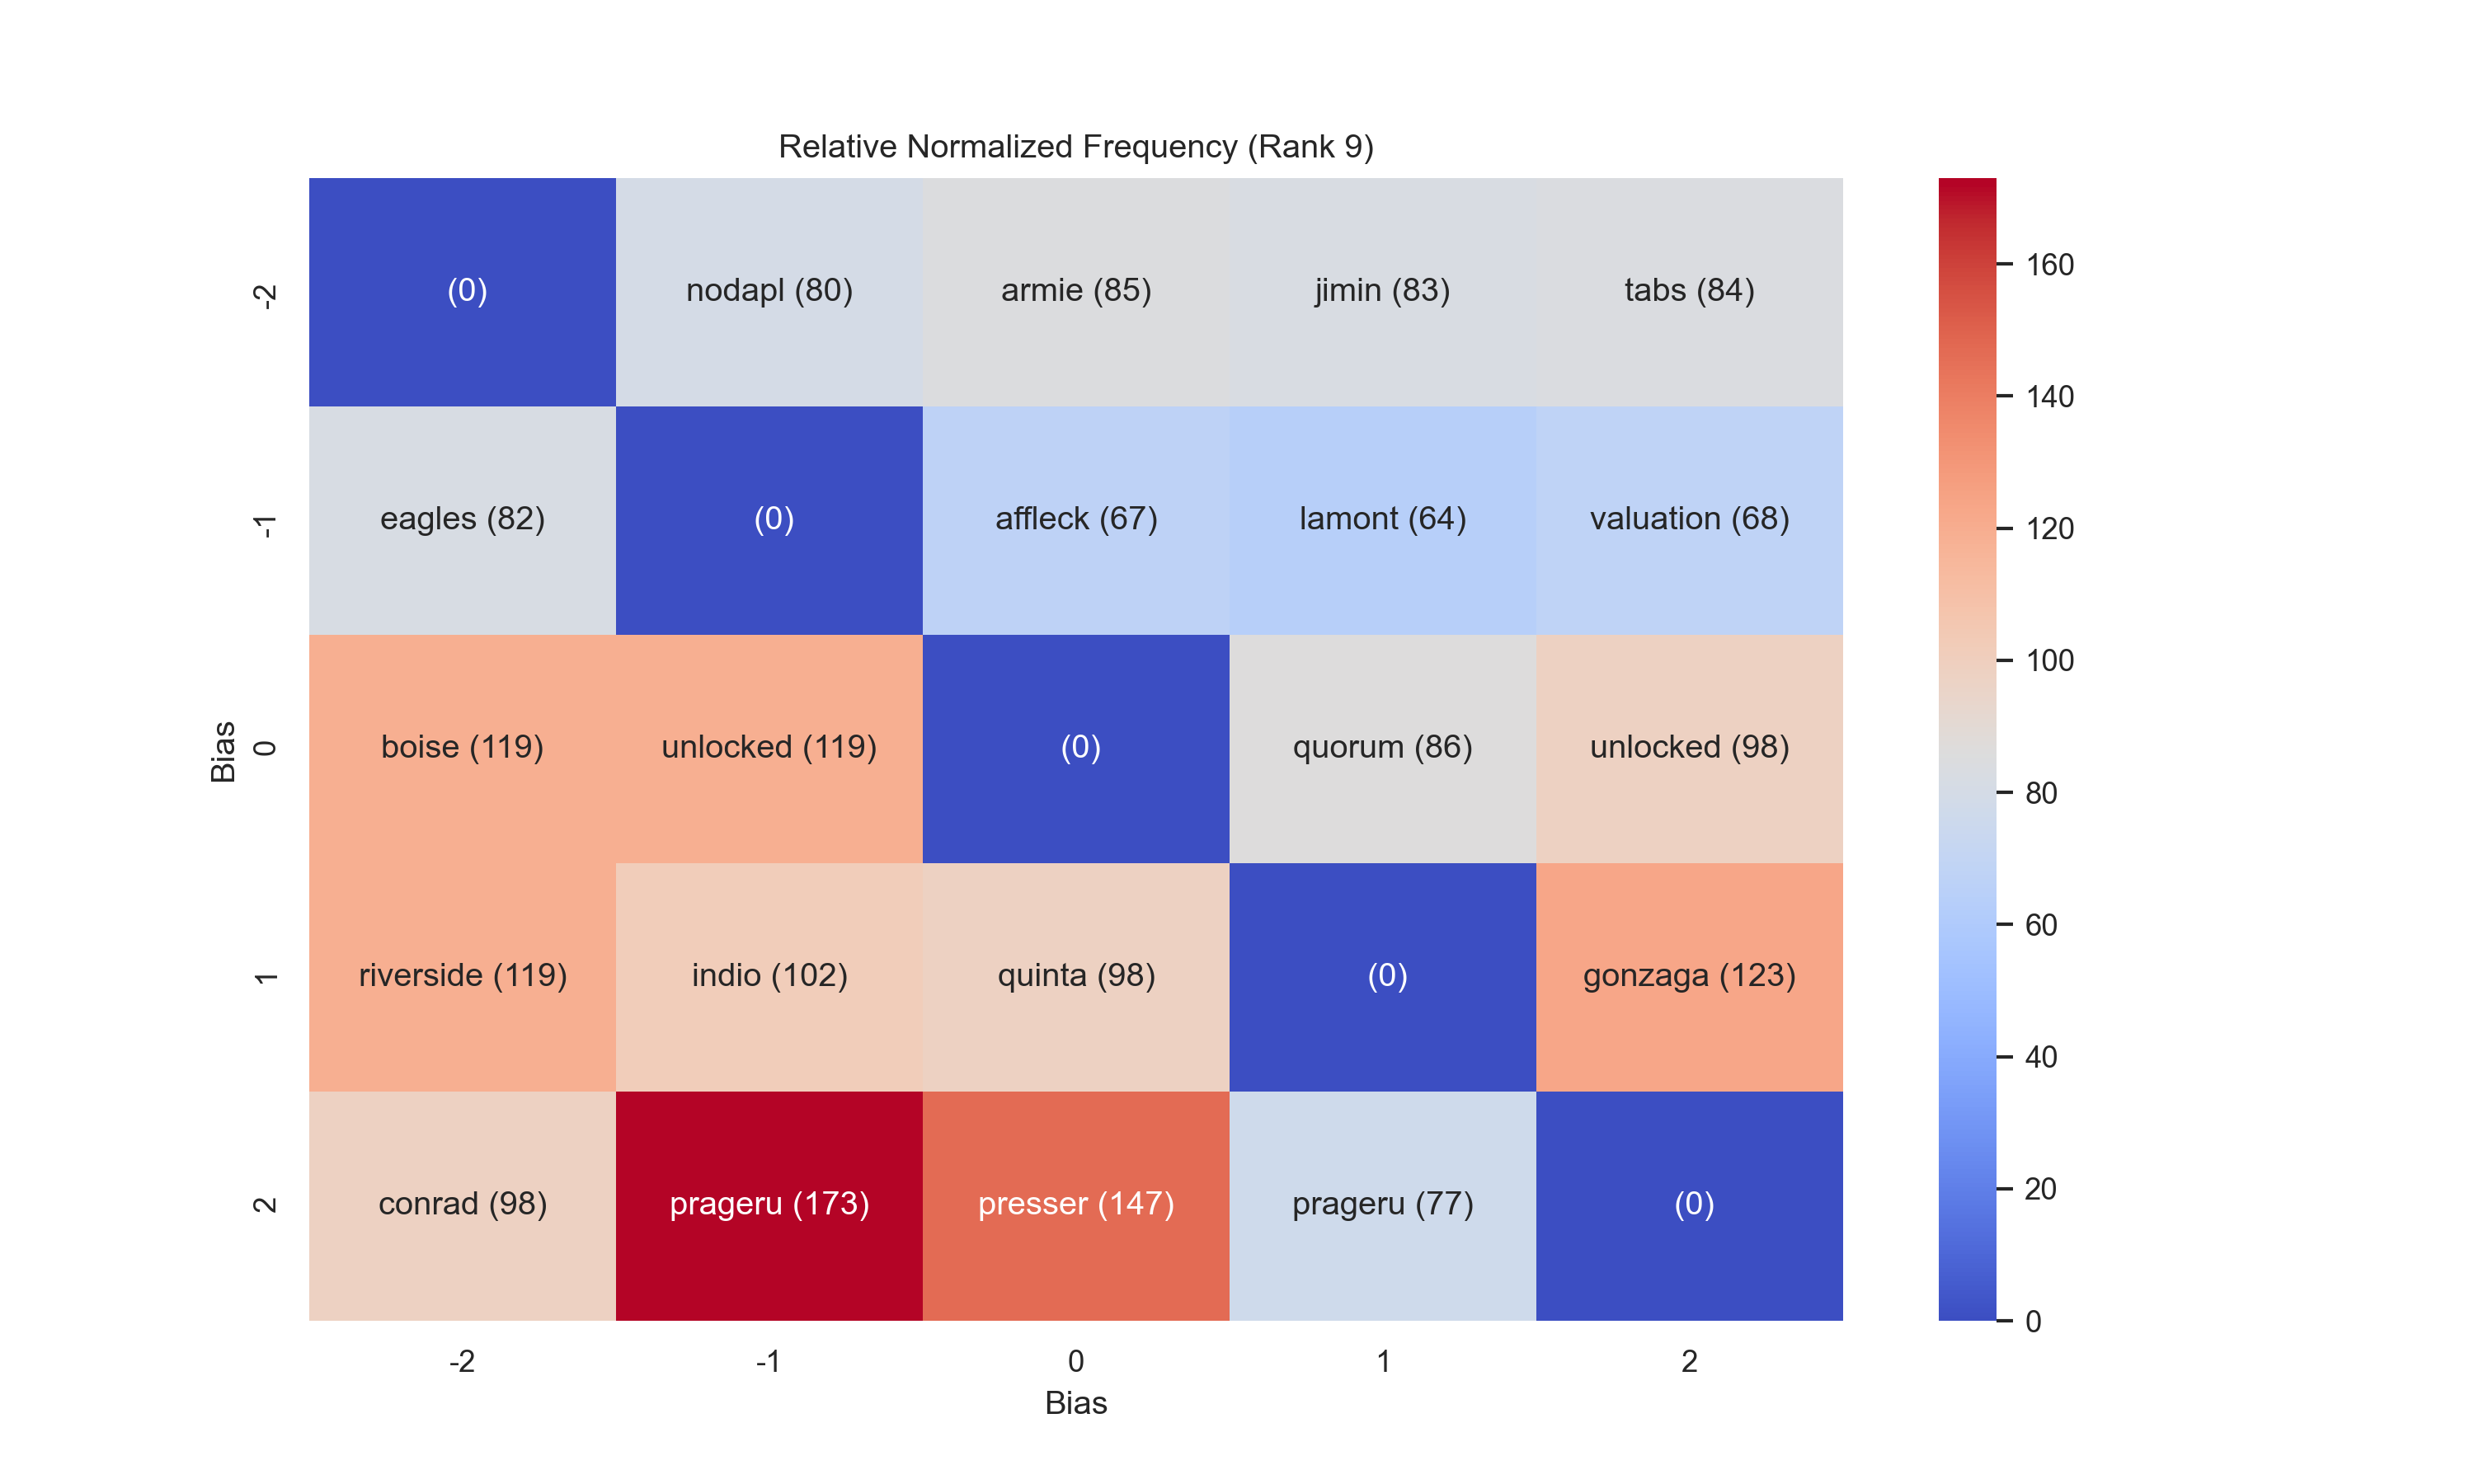
\includegraphics[width=0.6\textwidth]{figs/top_ten_rnf/rnf_w_rank_9.png}
\end{figure}
\end{center}

\pagebreak

\subsection{Top Ten Tokens Based on TF-IDF}
\subsubsection{Bias Class -2 (Left)}
\begin{center}

\CatchFileDef{\TTTFIDFTable}{figs/top_ten_tf_idf/table_-2_token.latex.txt}

\TTTFIDFTable
\begin{figure}[h!]
  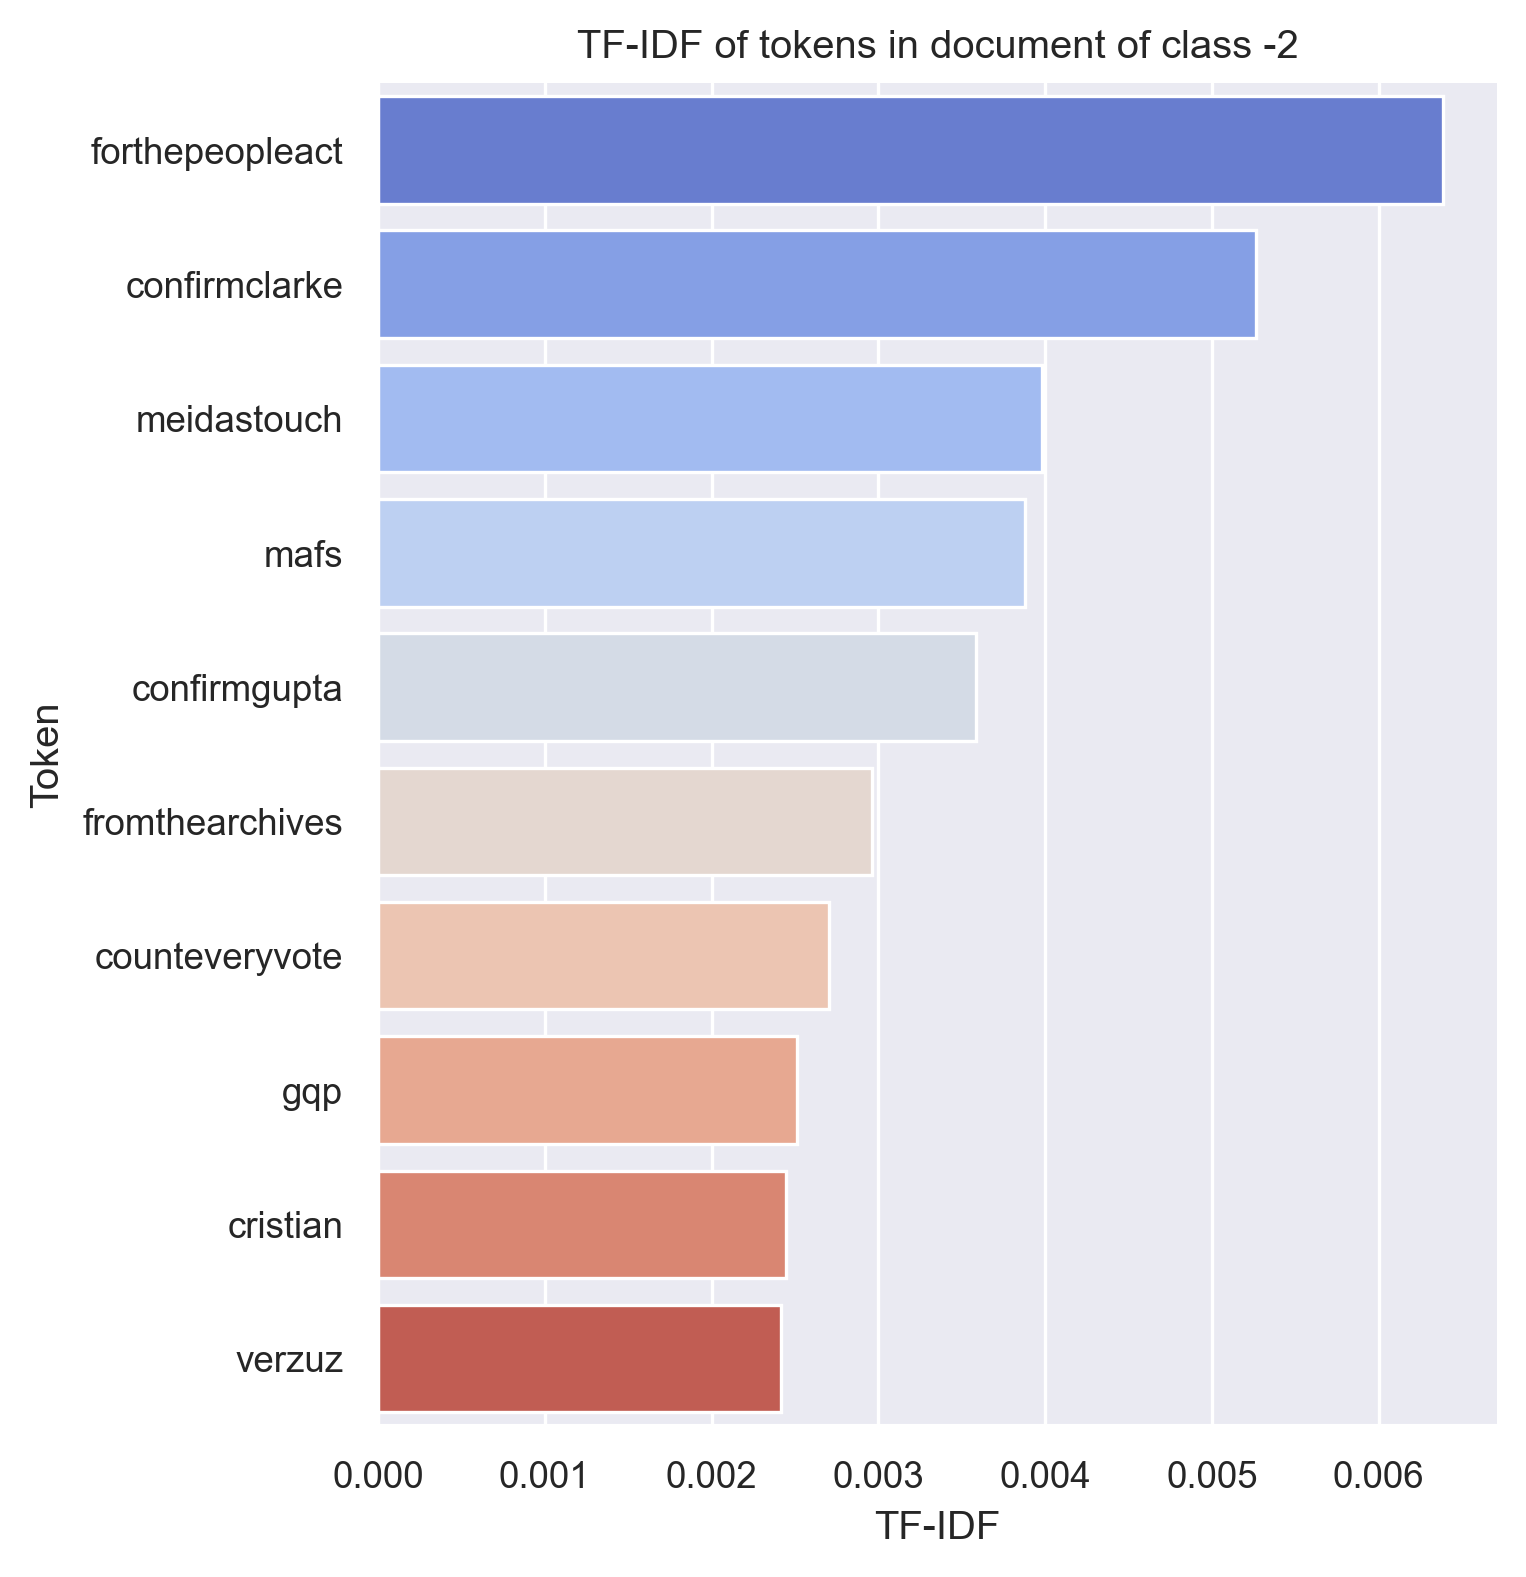
\includegraphics[width=0.65\textwidth]{figs/top_ten_tf_idf/tf_idf_token_-2.png}
\end{figure}
\end{center}

\pagebreak

\subsubsection{Bias Class -1 (Center-Left)}
\begin{center}

\CatchFileDef{\TTTFIDFTable}{figs/top_ten_tf_idf/table_-1_token.latex.txt}

\TTTFIDFTable
\begin{figure}[h!]
  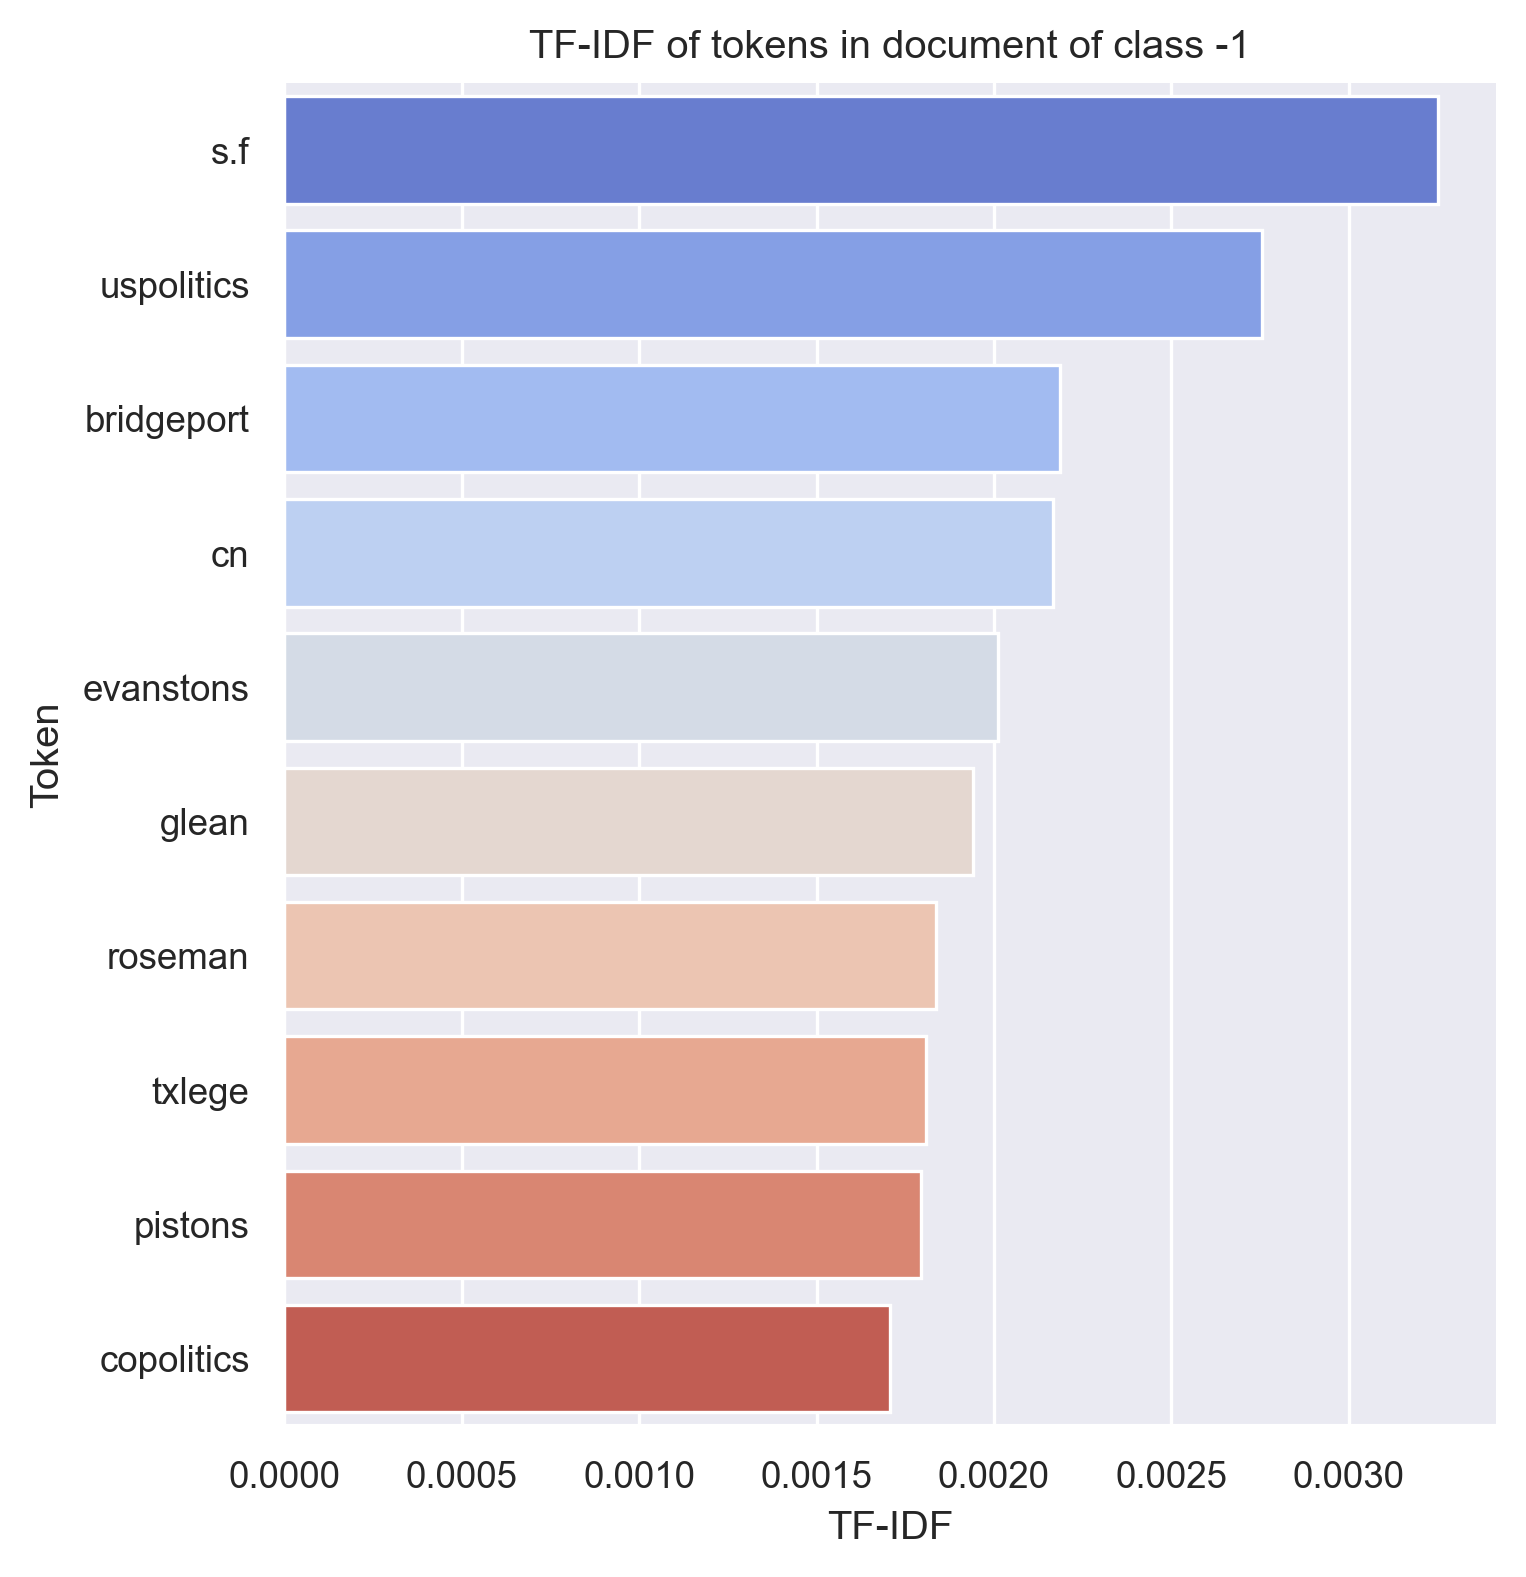
\includegraphics[width=0.65\textwidth]{figs/top_ten_tf_idf/tf_idf_token_-1.png}
\end{figure}
\end{center}

\pagebreak

\subsubsection{Bias Class 0 (Center)}
\begin{center}

\CatchFileDef{\TTTFIDFTable}{figs/top_ten_tf_idf/table_0_token.latex.txt}

\TTTFIDFTable
\begin{figure}[h!]
  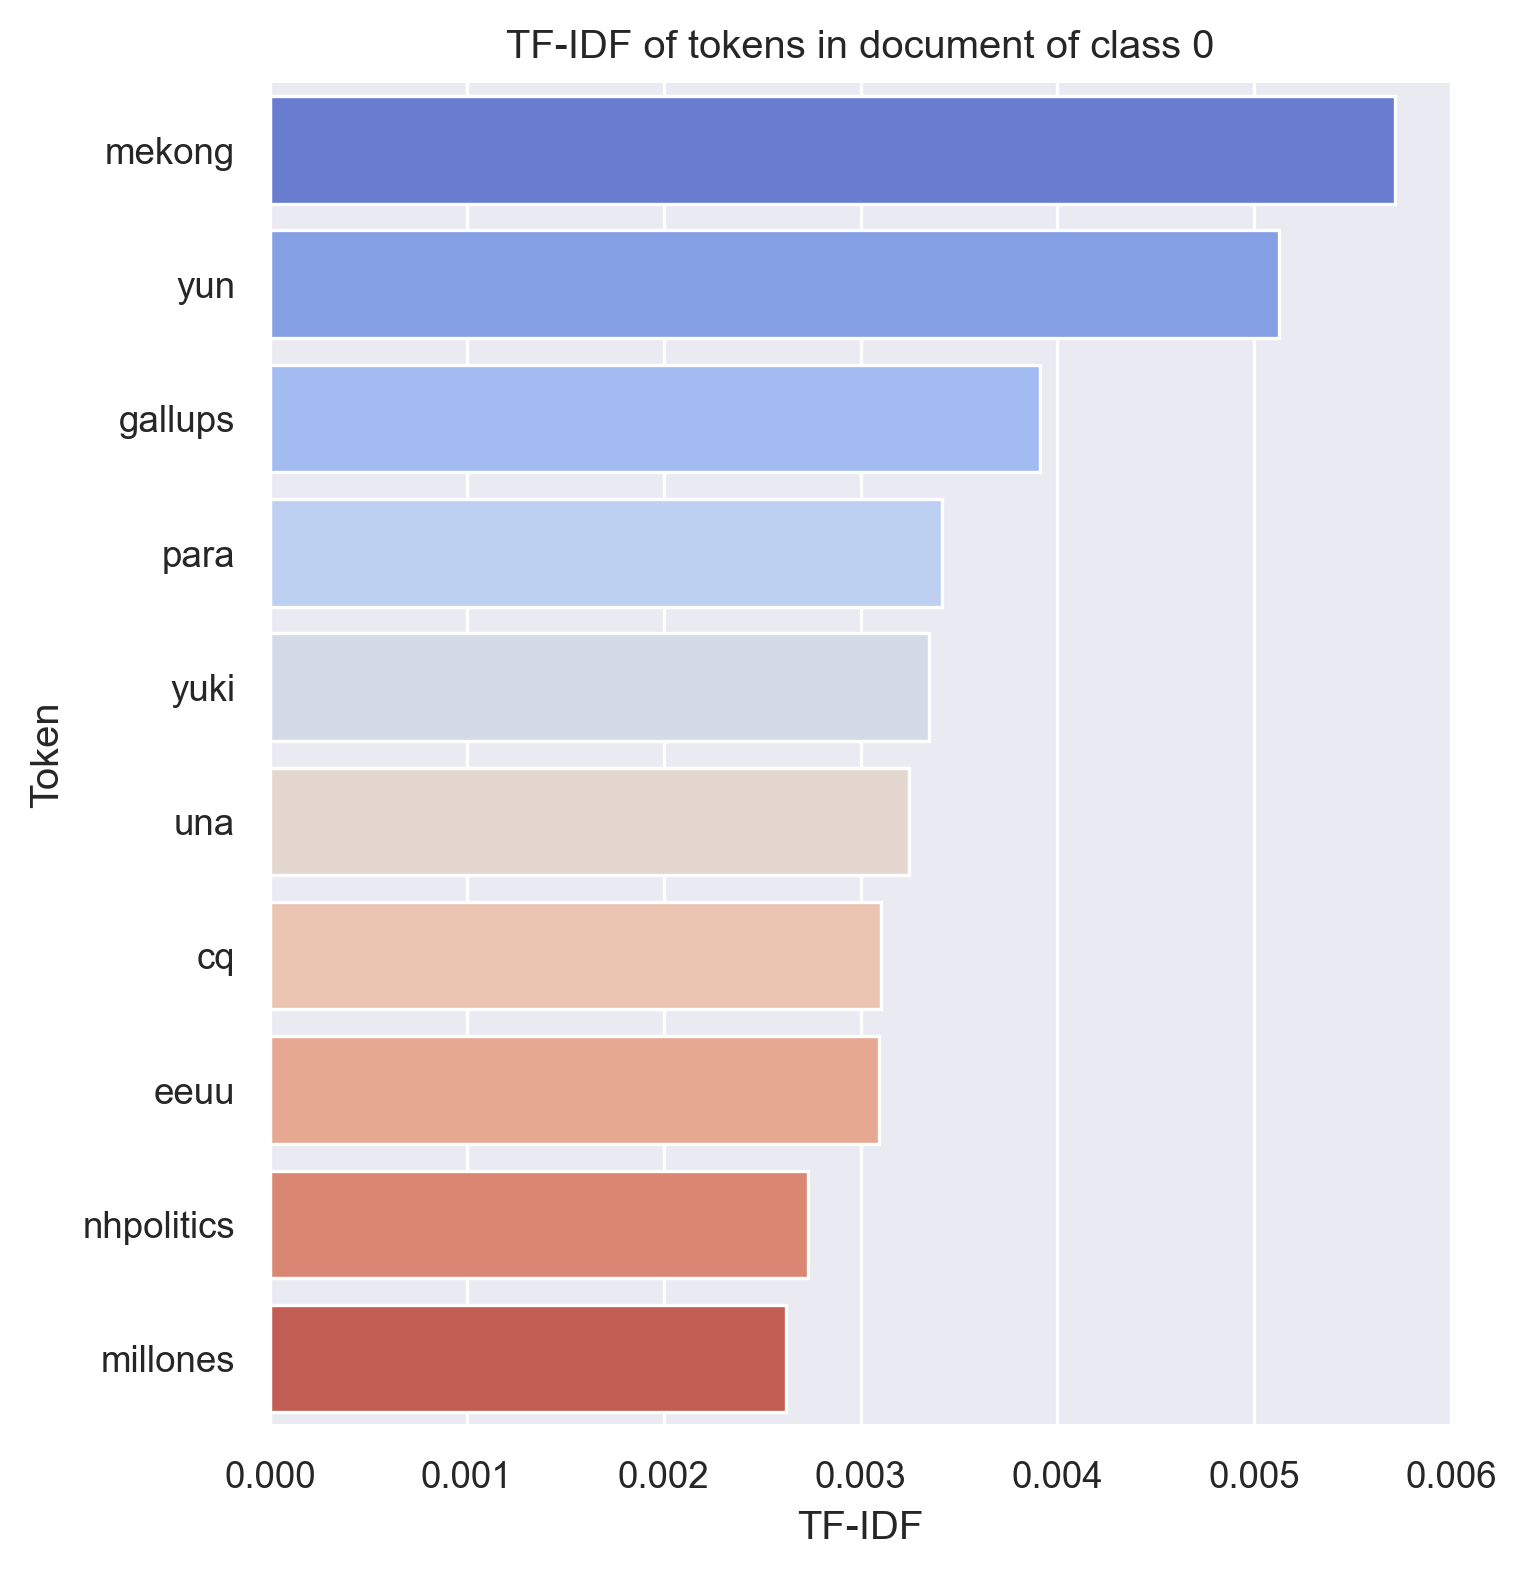
\includegraphics[width=0.65\textwidth]{figs/top_ten_tf_idf/tf_idf_token_0.png}
\end{figure}
\end{center}

\pagebreak

\subsubsection{Bias Class 1 (Center-Right)}
\begin{center}

\CatchFileDef{\TTTFIDFTable}{figs/top_ten_tf_idf/table_1_token.latex.txt}

\TTTFIDFTable
\begin{figure}[h!]
  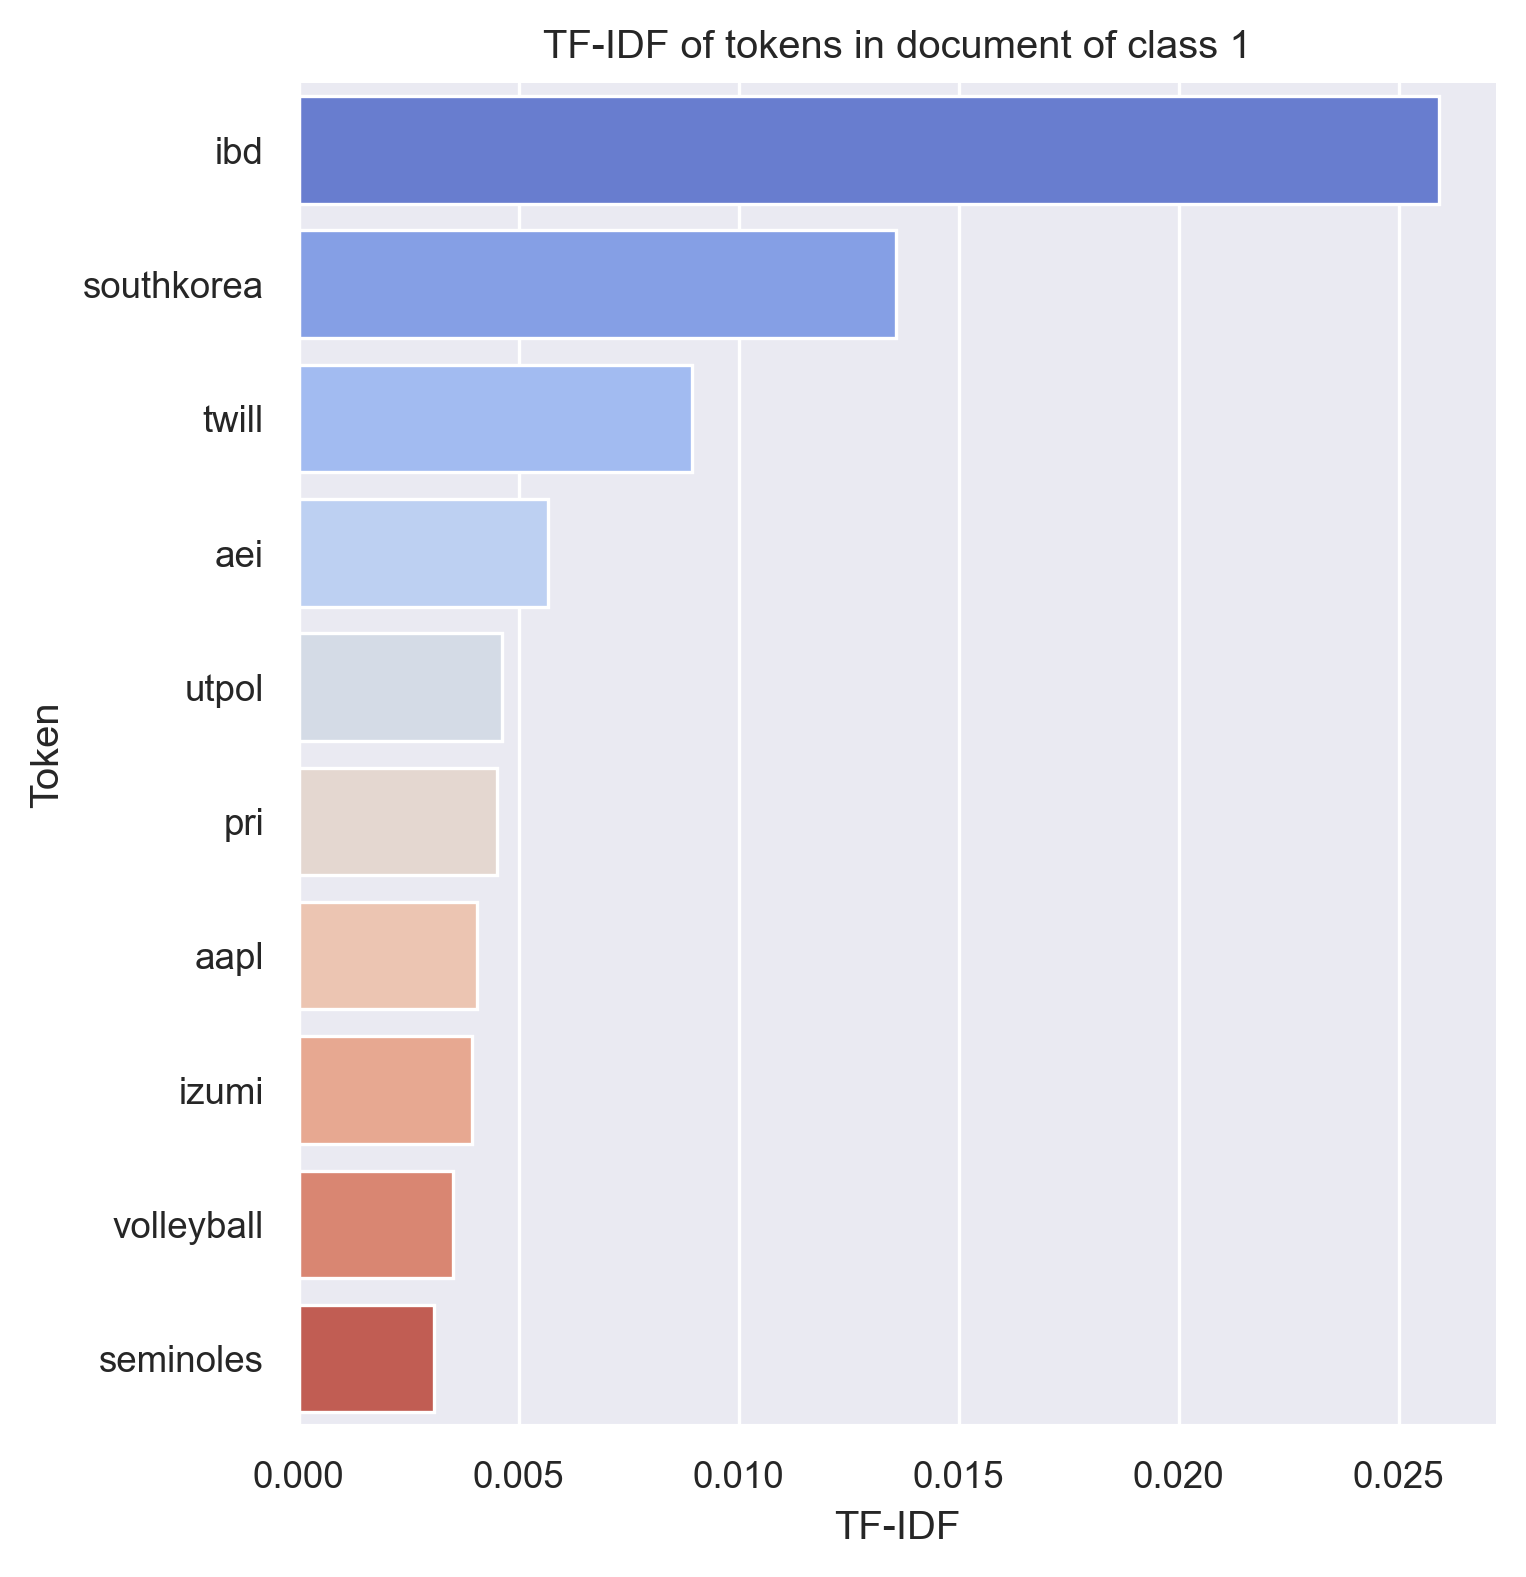
\includegraphics[width=0.65\textwidth]{figs/top_ten_tf_idf/tf_idf_token_1.png}
\end{figure}
\end{center}

\pagebreak

\subsubsection{Bias Class 2 (Right)}
\begin{center}

\CatchFileDef{\TTTFIDFTable}{figs/top_ten_tf_idf/table_2_token.latex.txt}

\TTTFIDFTable
\begin{figure}[h!]
  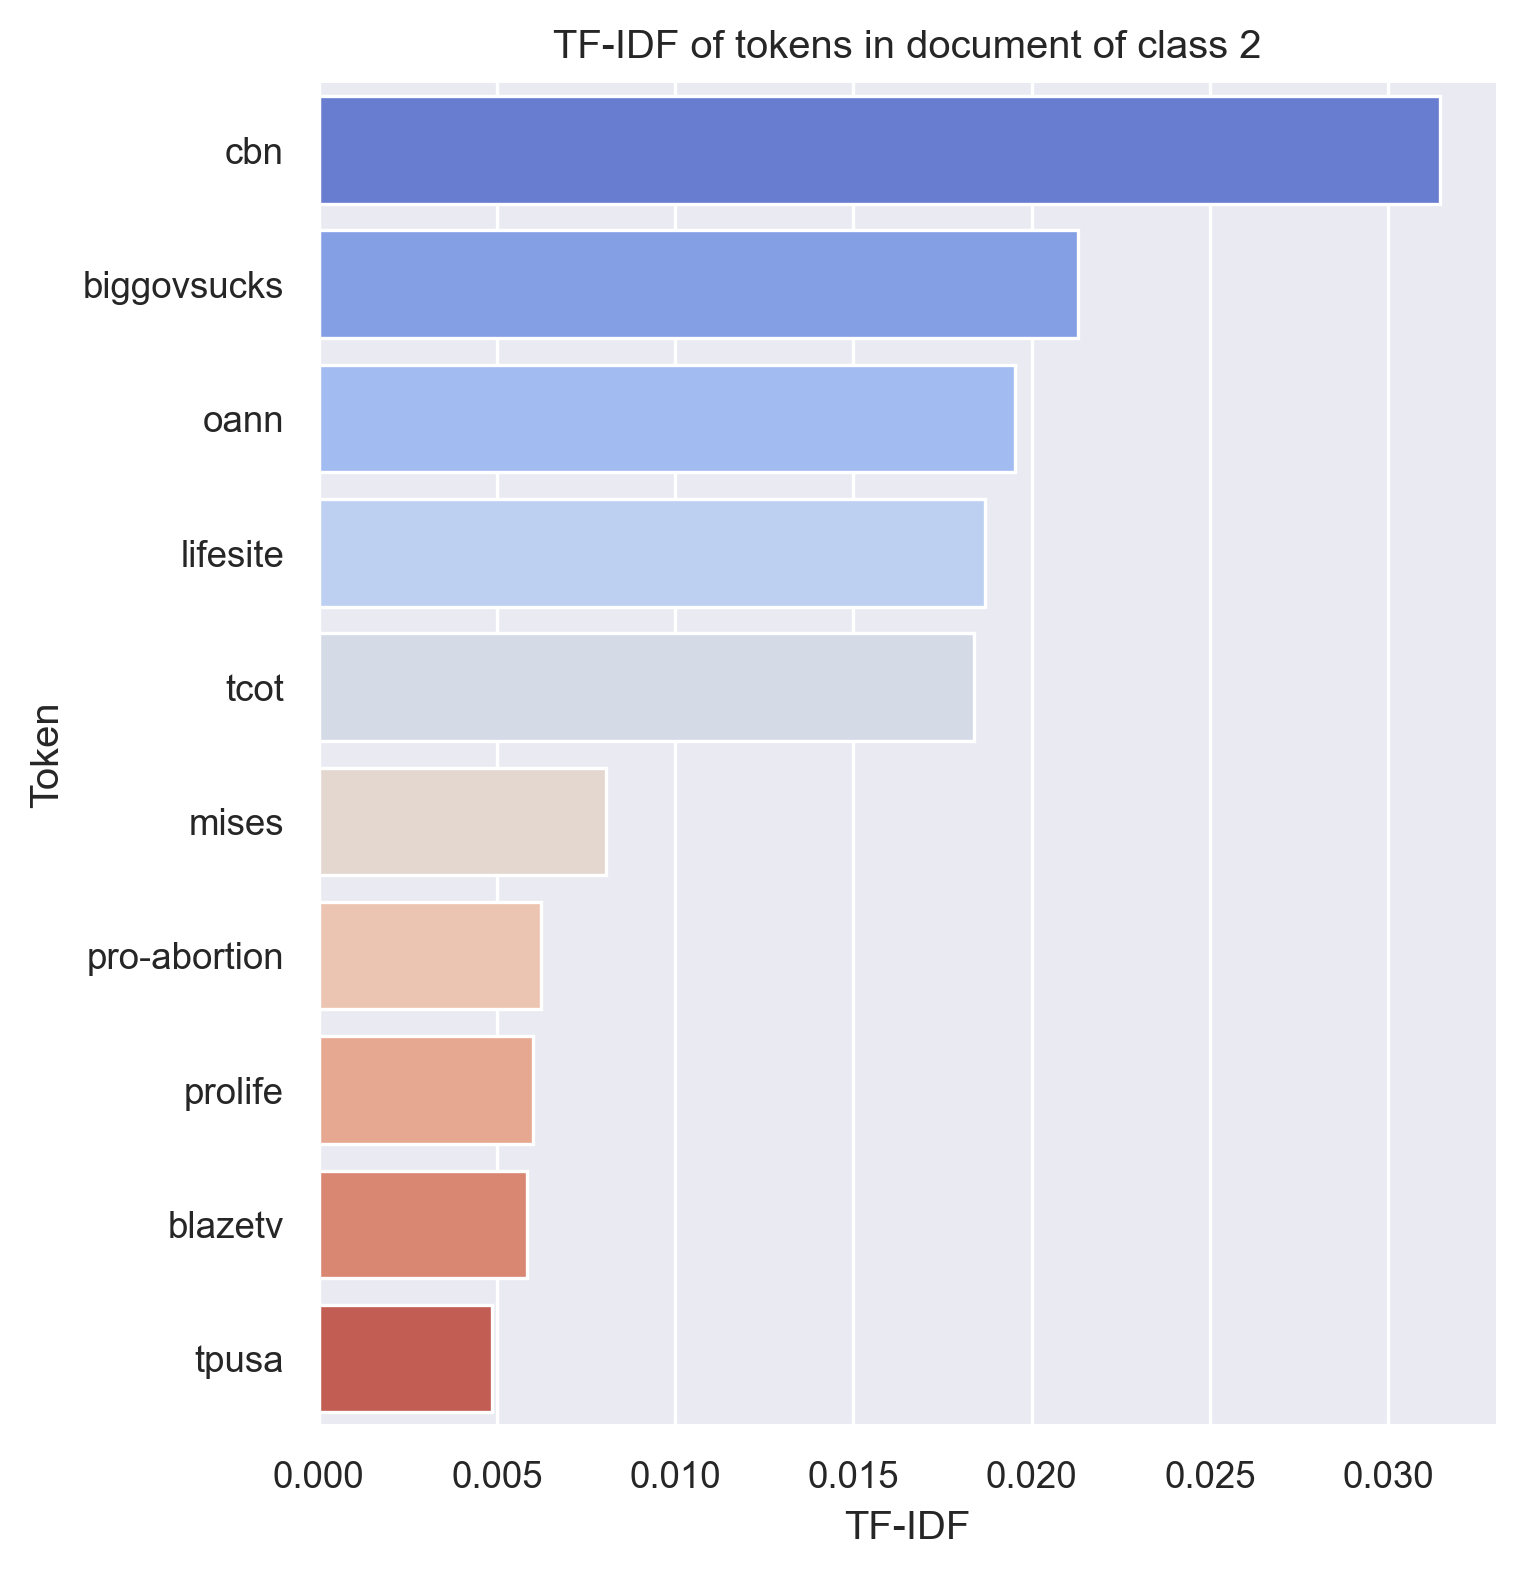
\includegraphics[width=0.65\textwidth]{figs/top_ten_tf_idf/tf_idf_token_2.png}
\end{figure}
\end{center}

\pagebreak

\subsection{Top Ten Words Based on TF-IDF}
\subsubsection{Bias Class -2 (Left)}
\begin{center}

\CatchFileDef{\TTTFIDFTable}{figs/top_ten_tf_idf/table_-2_word.latex.txt}

\TTTFIDFTable
\begin{figure}[h!]
  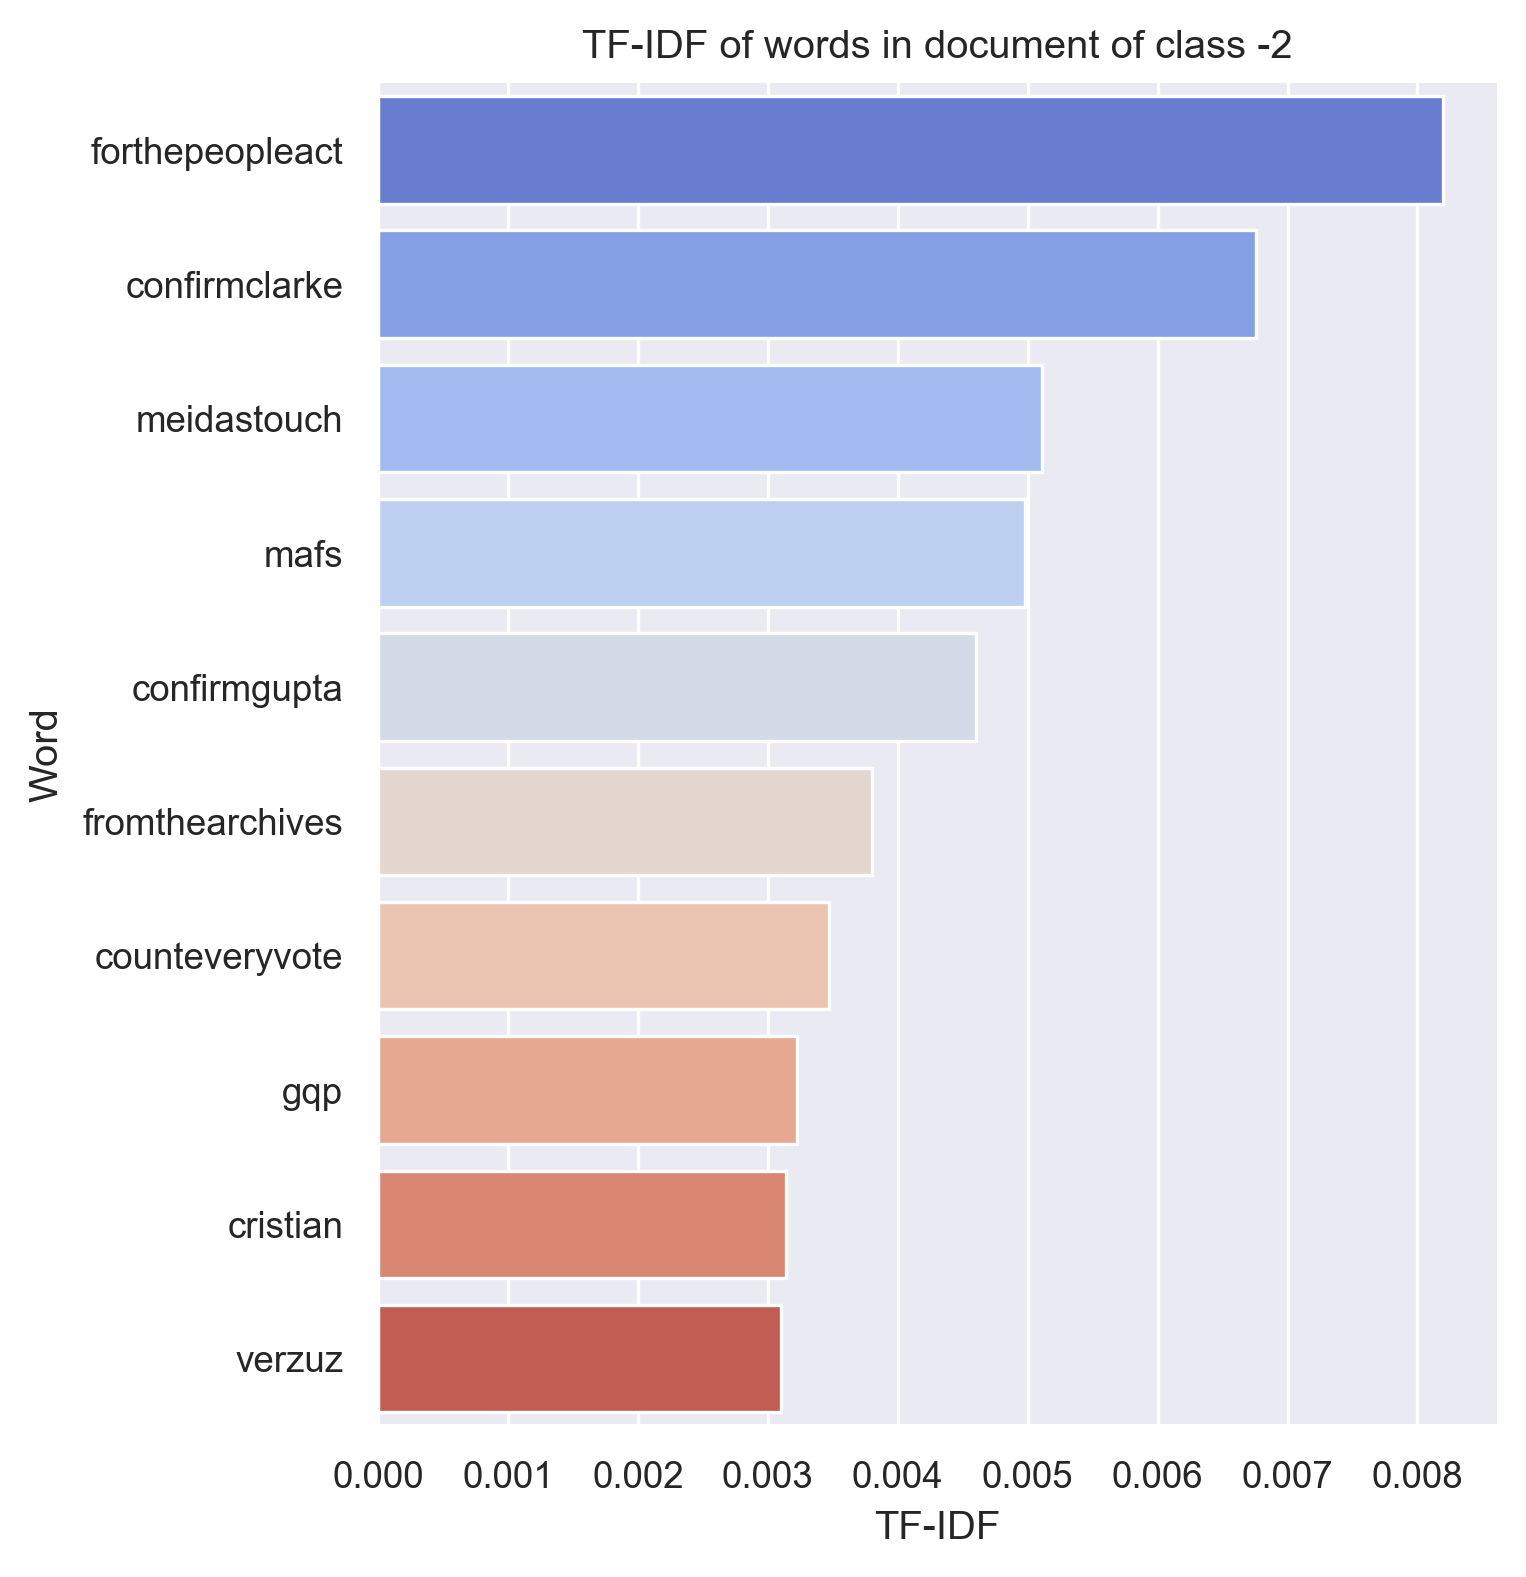
\includegraphics[width=0.65\textwidth]{figs/top_ten_tf_idf/tf_idf_word_-2.png}
\end{figure}
\end{center}

\pagebreak

\subsubsection{Bias Class -1 (Center-Left)}
\begin{center}

\CatchFileDef{\TTTFIDFTable}{figs/top_ten_tf_idf/table_-1_word.latex.txt}

\TTTFIDFTable
\begin{figure}[h!]
  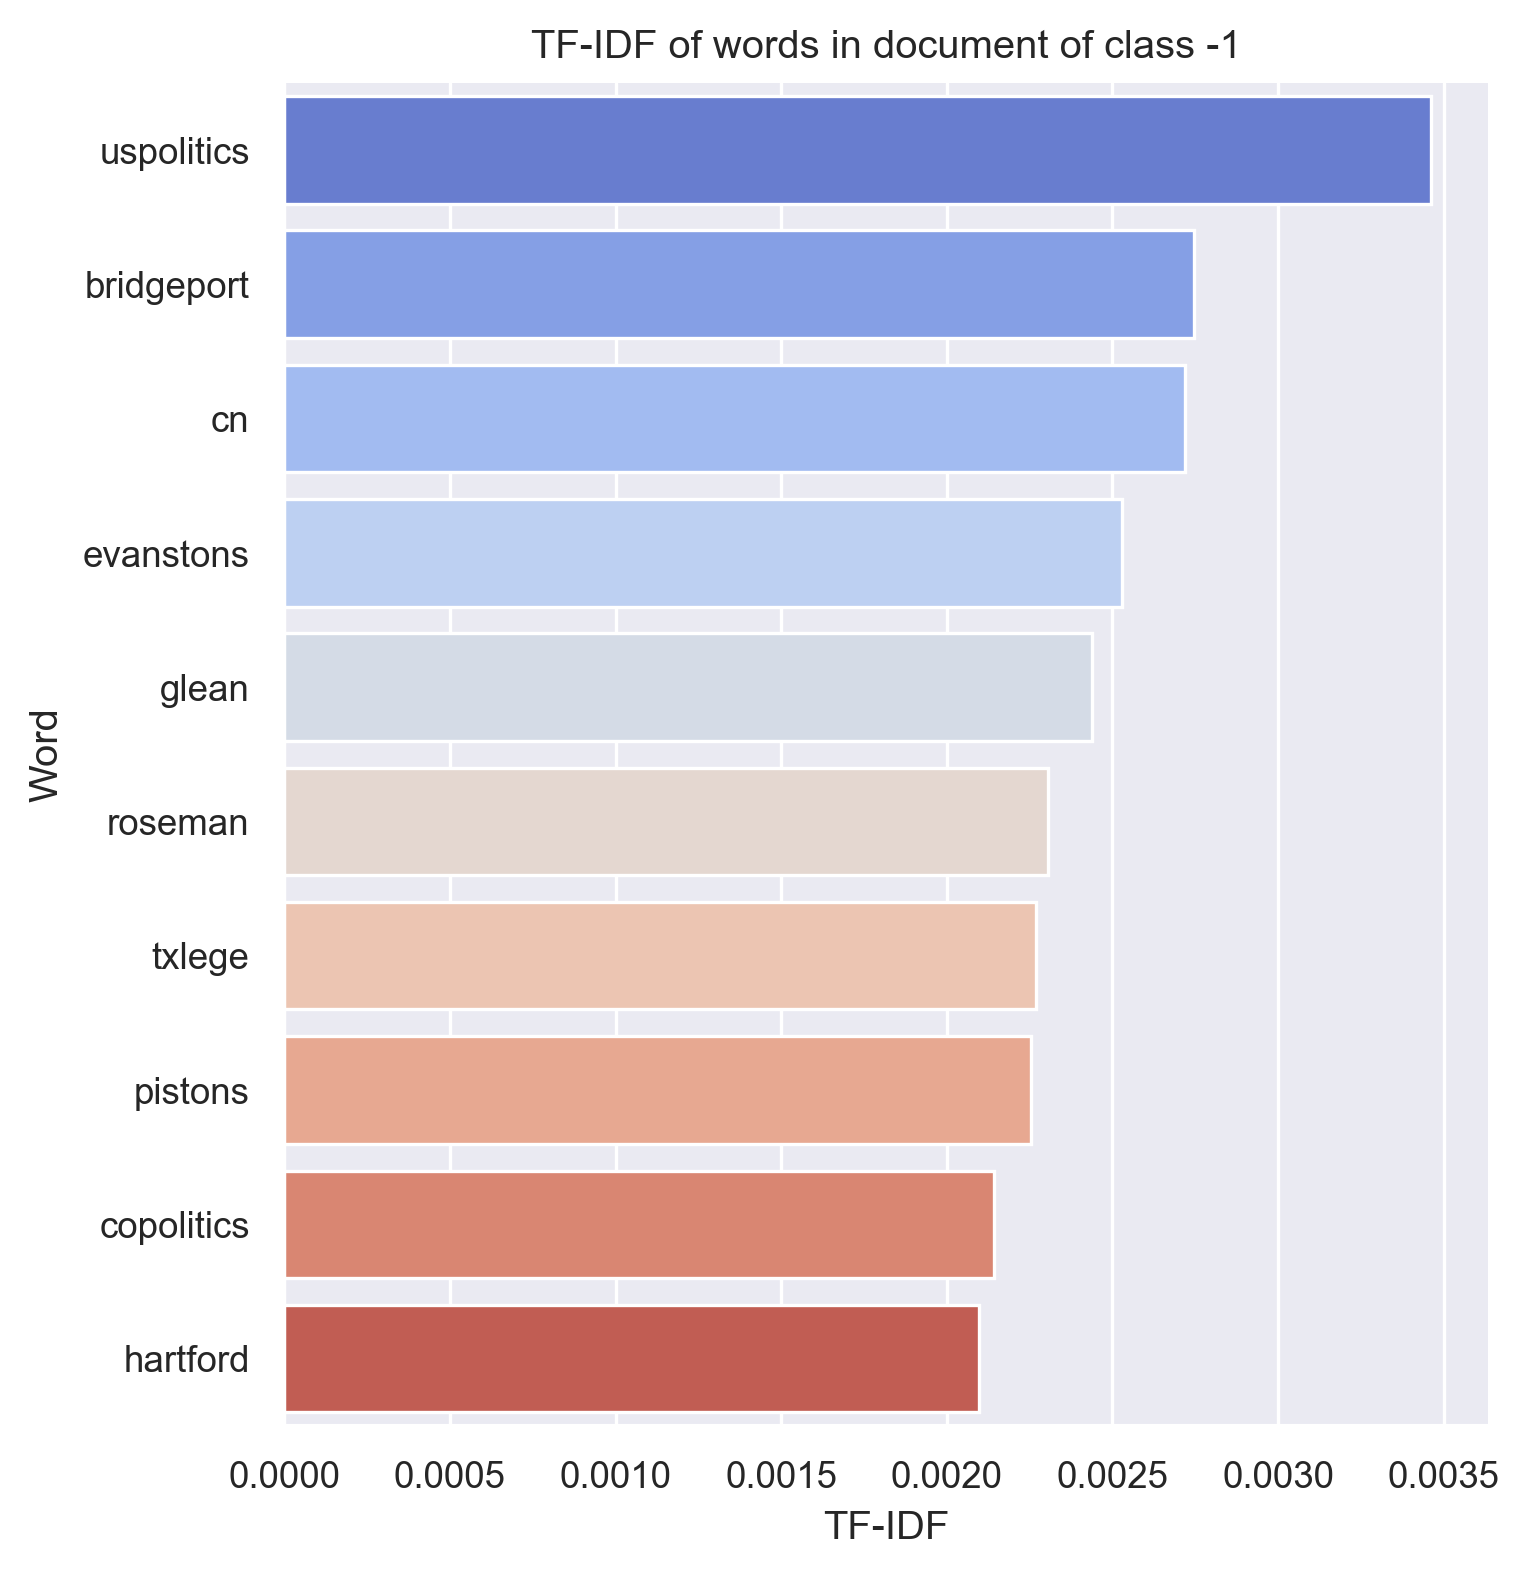
\includegraphics[width=0.65\textwidth]{figs/top_ten_tf_idf/tf_idf_word_-1.png}
\end{figure}
\end{center}

\pagebreak

\subsubsection{Bias Class 0 (Center)}
\begin{center}

\CatchFileDef{\TTTFIDFTable}{figs/top_ten_tf_idf/table_0_word.latex.txt}

\TTTFIDFTable
\begin{figure}[h!]
  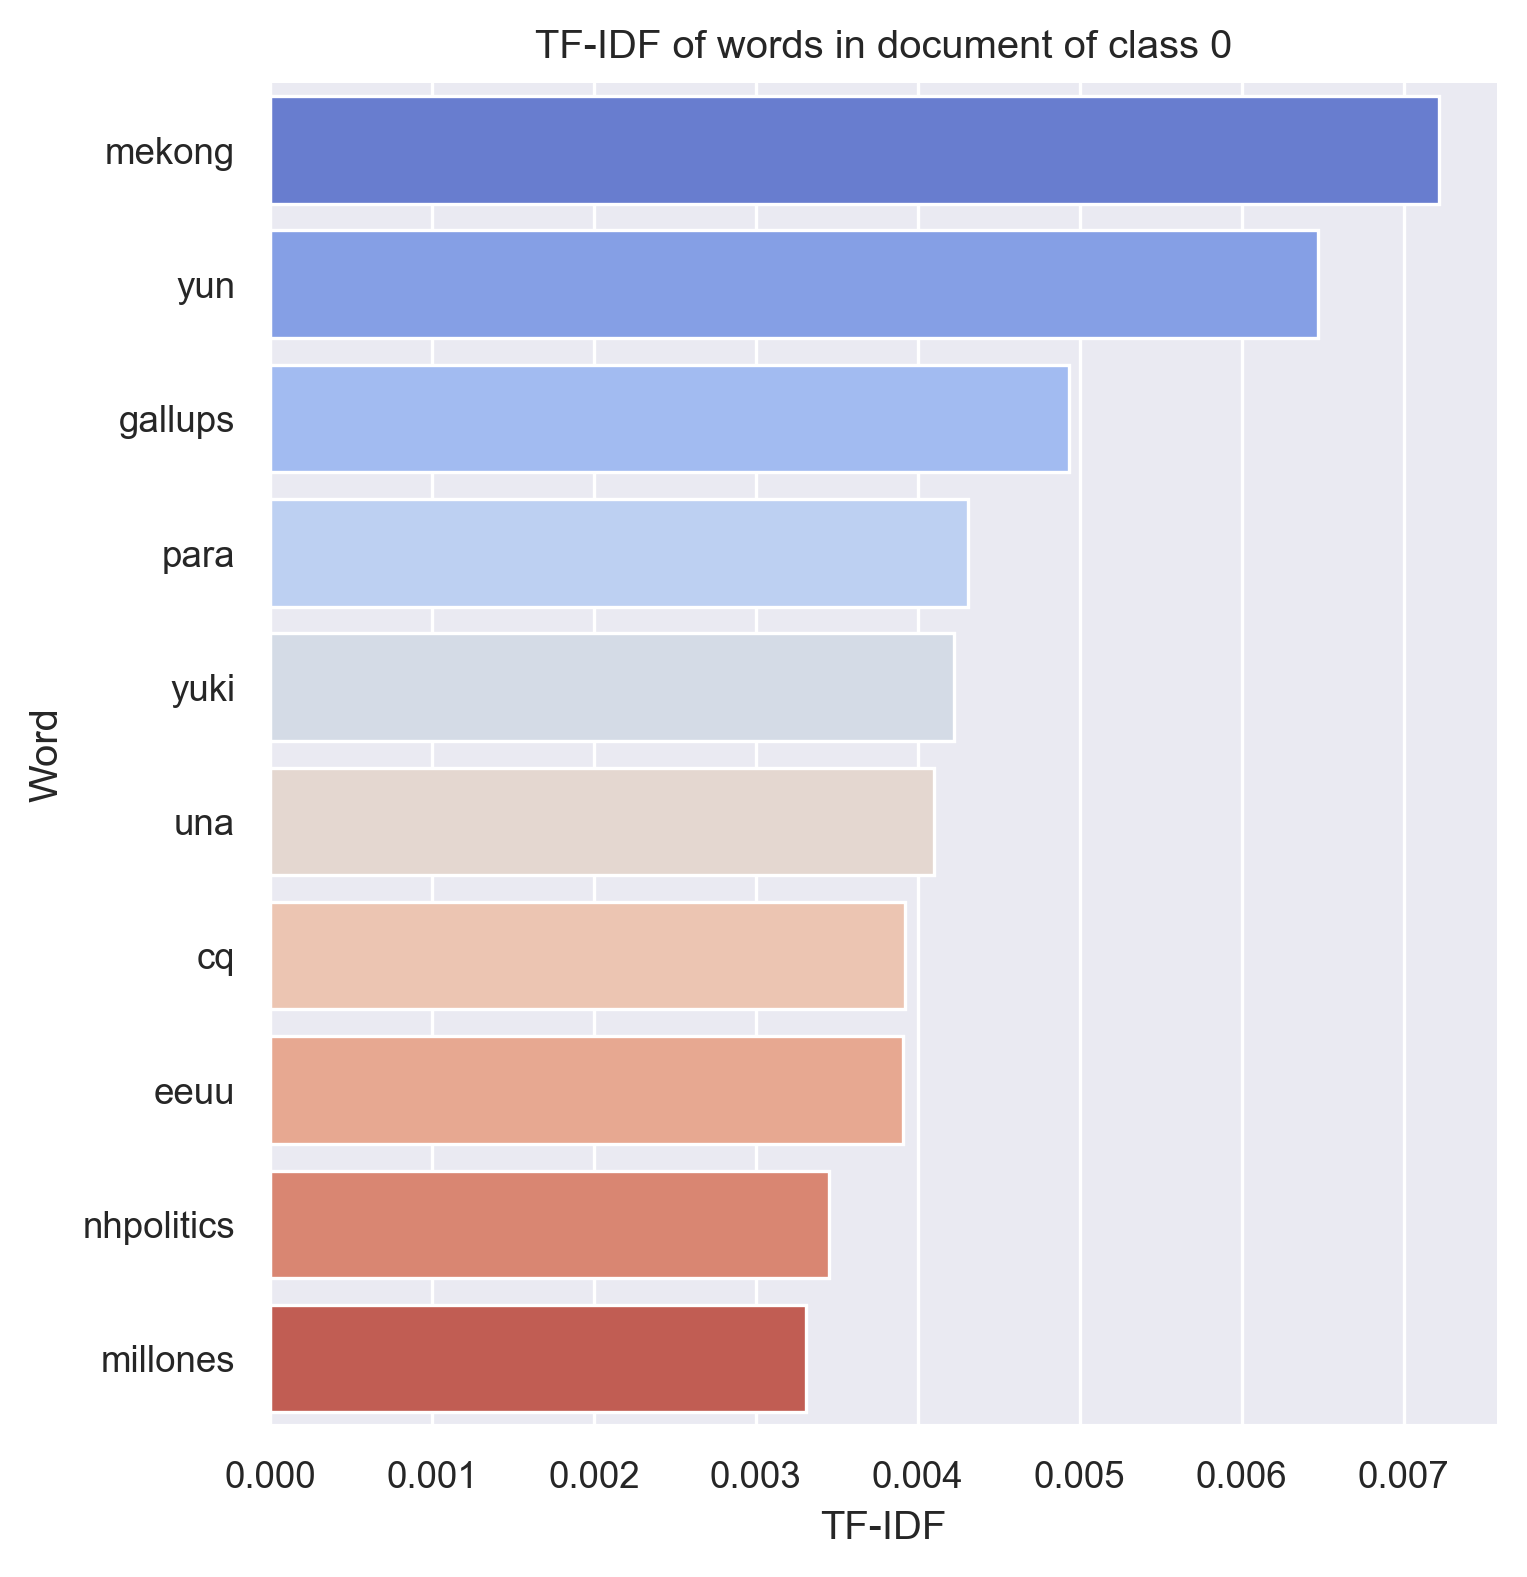
\includegraphics[width=0.65\textwidth]{figs/top_ten_tf_idf/tf_idf_word_0.png}
\end{figure}
\end{center}

\pagebreak

\subsubsection{Bias Class 1 (Center-Right)}
\begin{center}

\CatchFileDef{\TTTFIDFTable}{figs/top_ten_tf_idf/table_1_word.latex.txt}

\TTTFIDFTable
\begin{figure}[h!]
  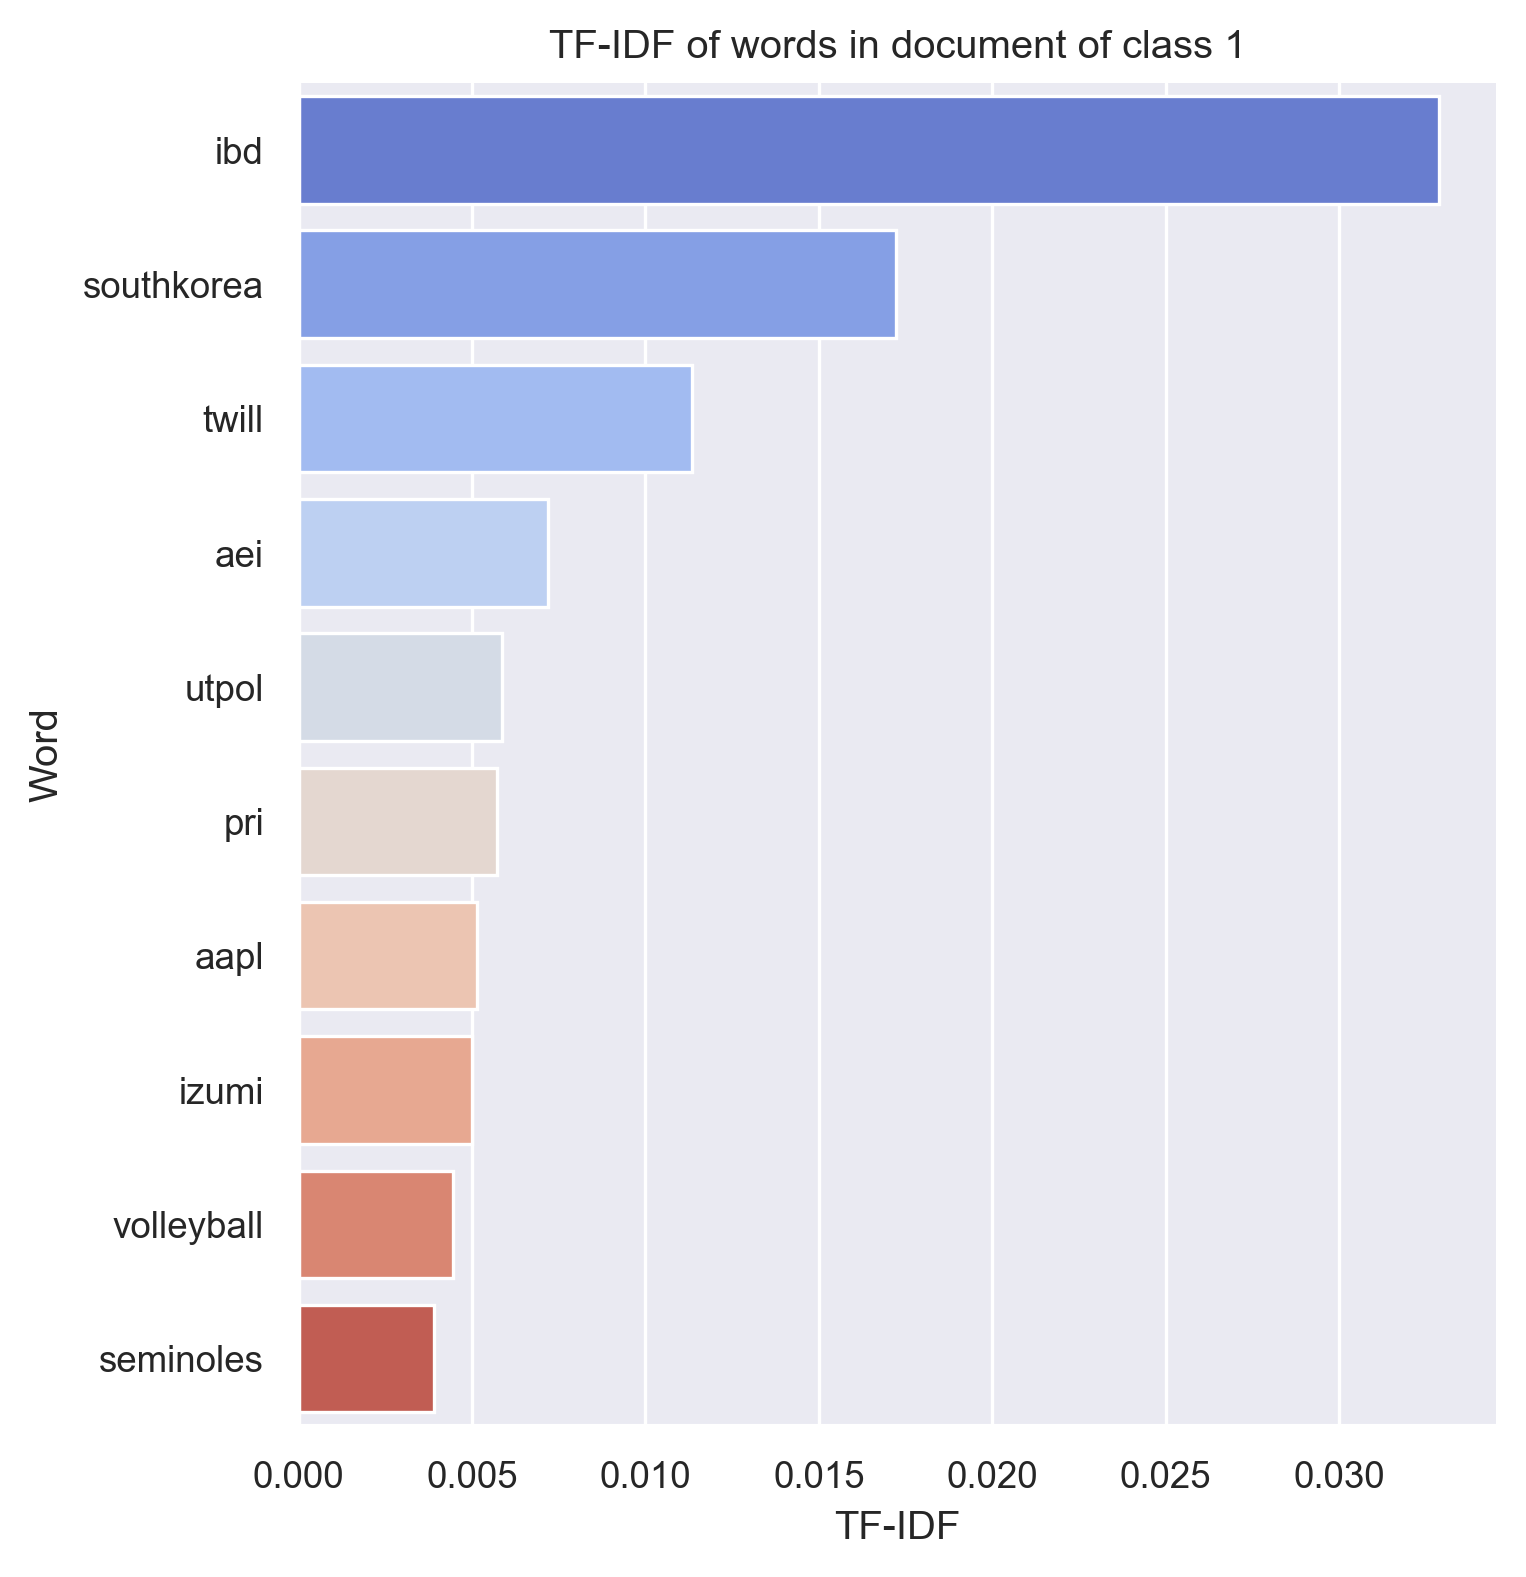
\includegraphics[width=0.65\textwidth]{figs/top_ten_tf_idf/tf_idf_word_1.png}
\end{figure}
\end{center}

\pagebreak

\subsubsection{Bias Class 2 (Right)}
\begin{center}

\CatchFileDef{\TTTFIDFTable}{figs/top_ten_tf_idf/table_2_word.latex.txt}

\TTTFIDFTable
\begin{figure}[h!]
  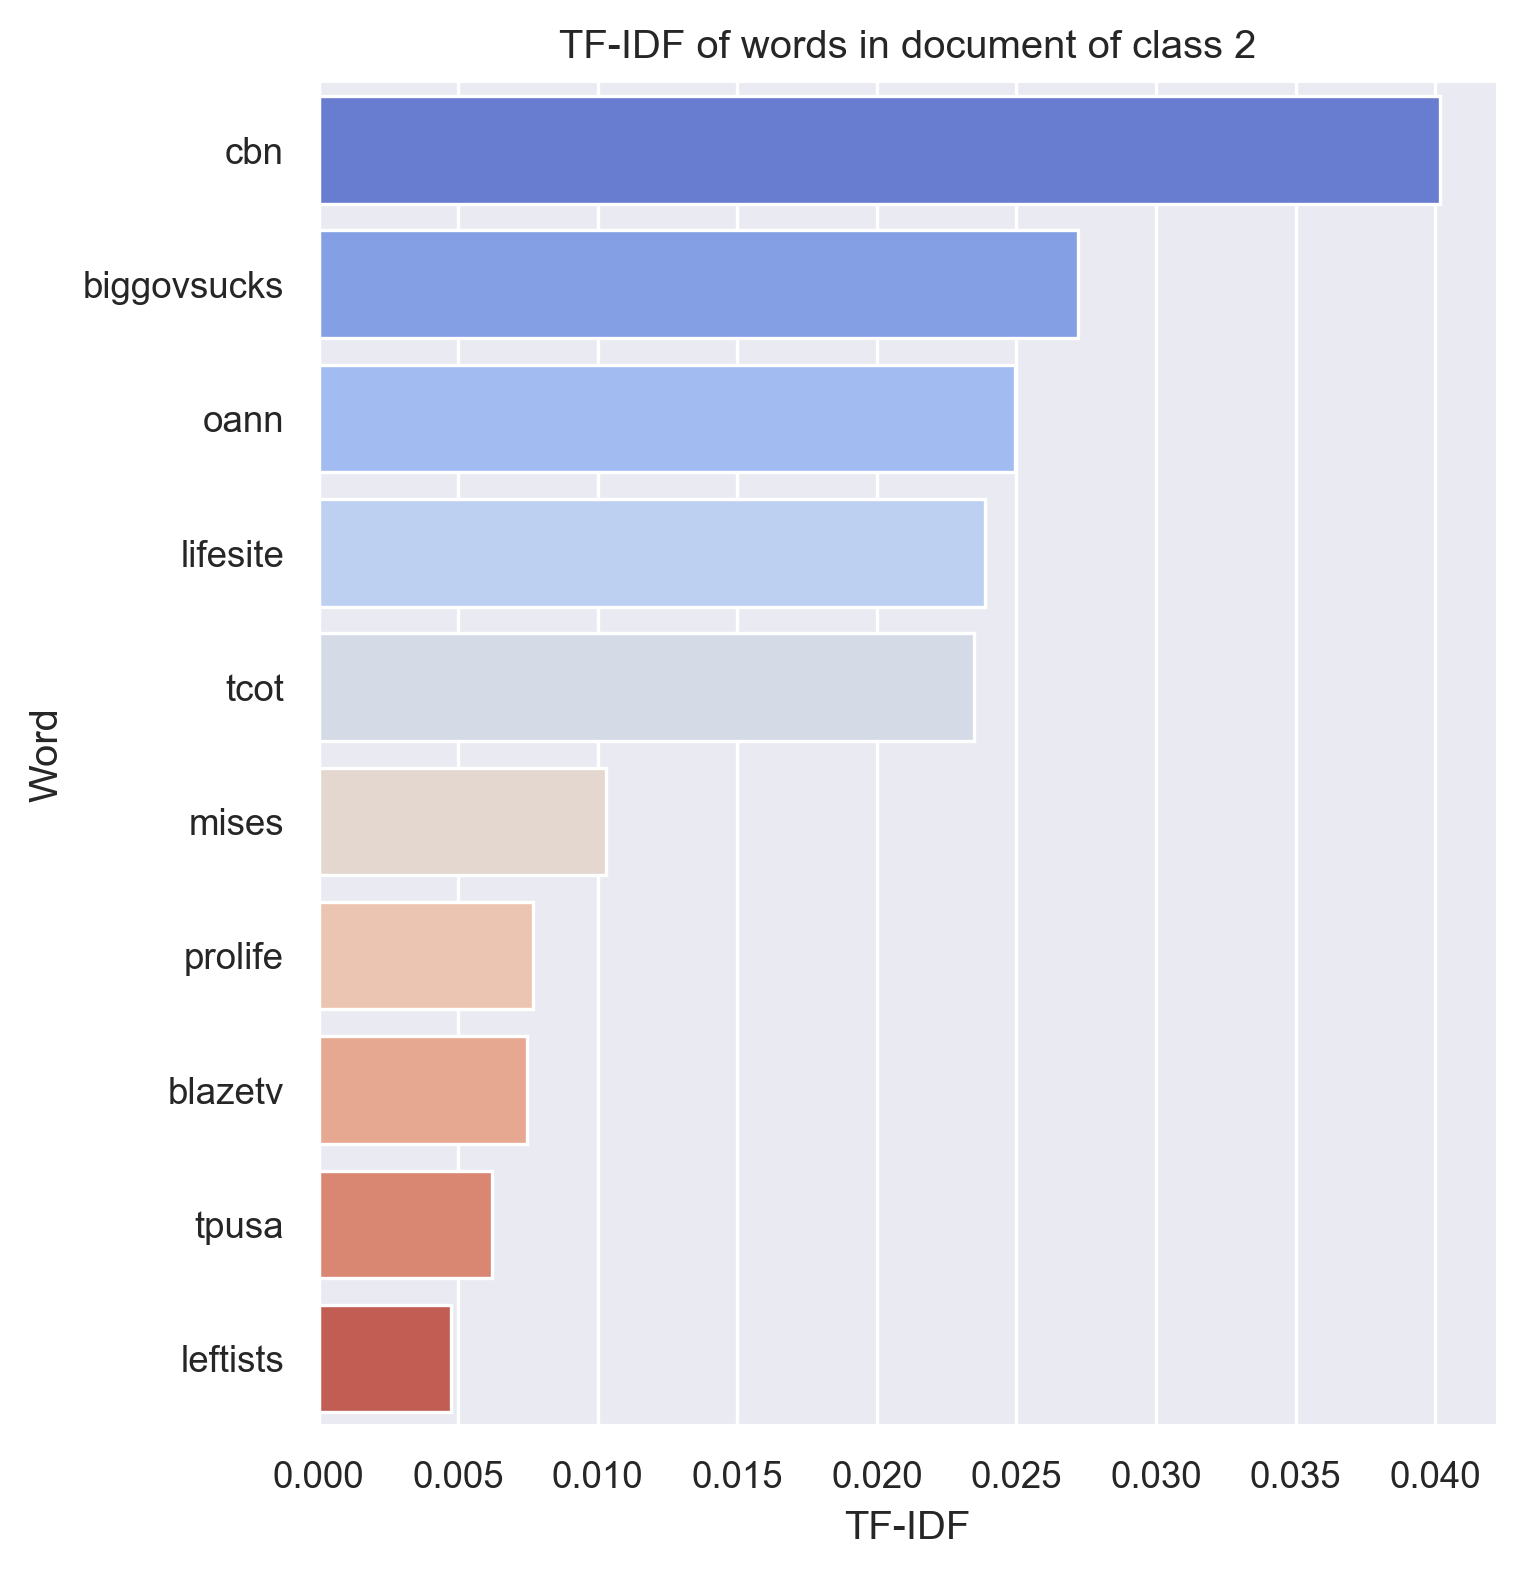
\includegraphics[width=0.65\textwidth]{figs/top_ten_tf_idf/tf_idf_word_2.png}
\end{figure}
\end{center}

\pagebreak

\subsection{Tokens Frequency Histogram}
\subsubsection{Bias Class -2 (Left)}
\begin{center}

\CatchFileDef{\TTTFIDFTable}{figs/words_histogram/table_-2_token.latex.txt}

\TTTFIDFTable
\begin{figure}[h!]
  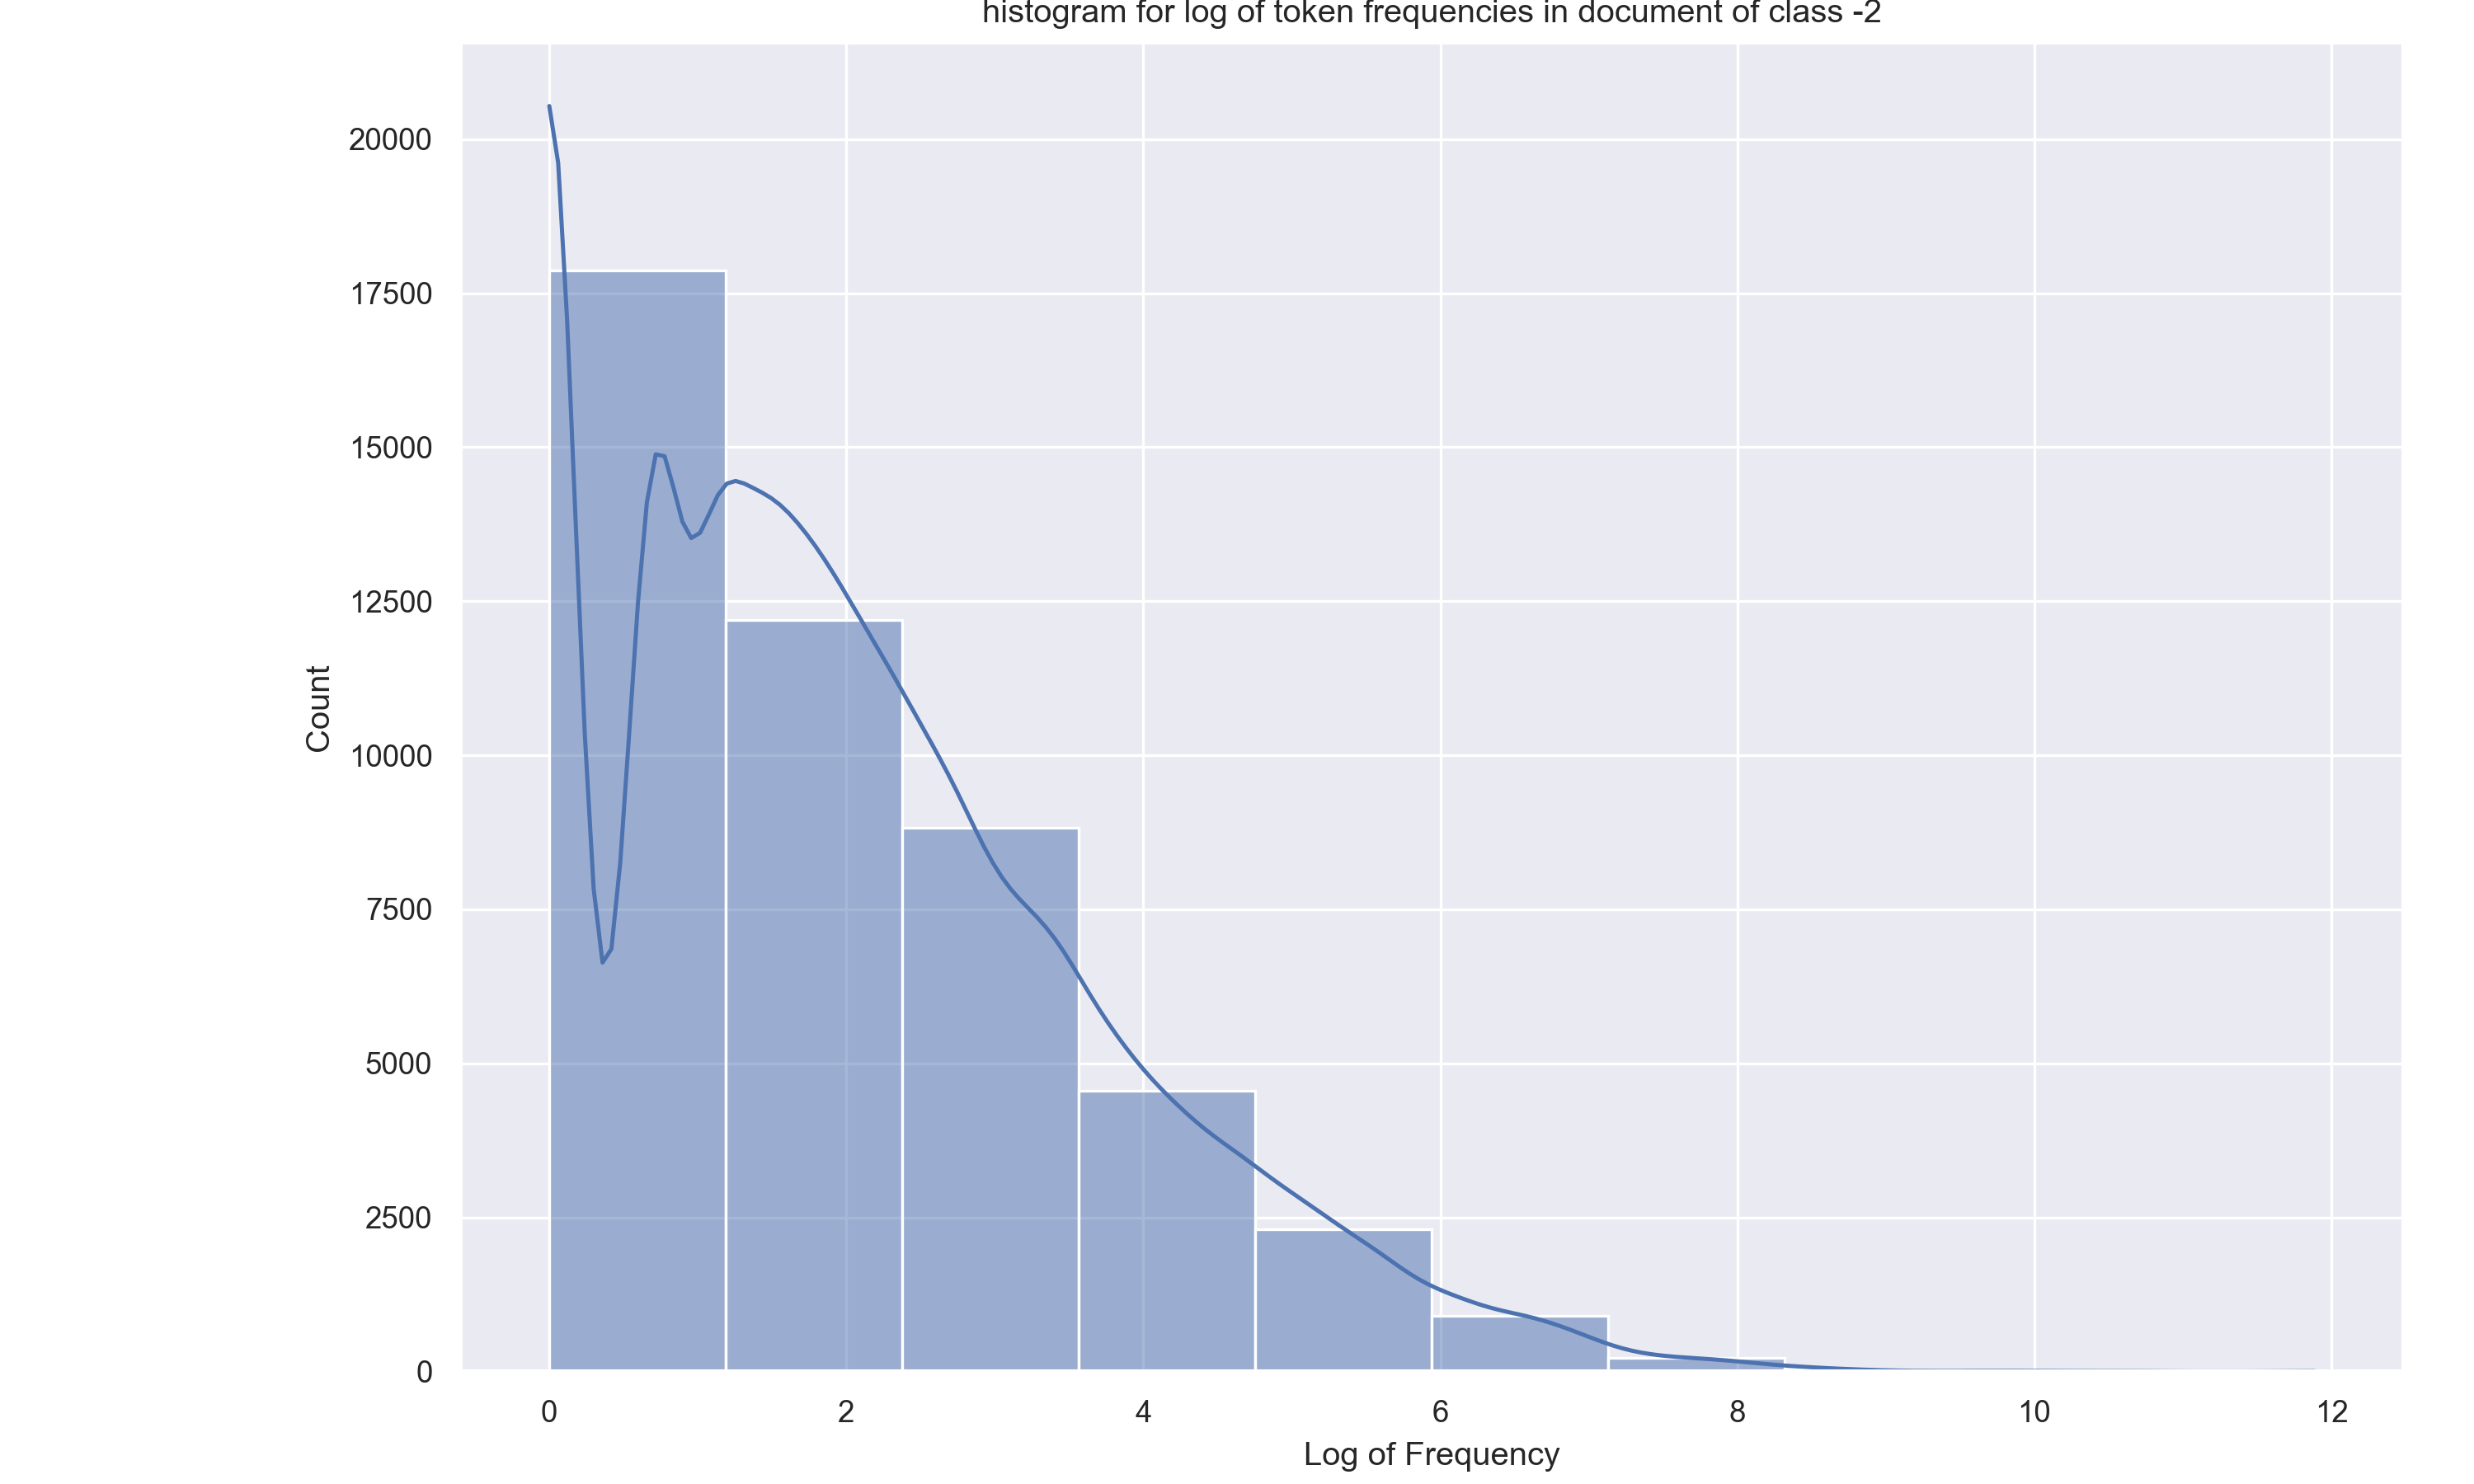
\includegraphics[width=0.65\textwidth]{figs/words_histogram/hist_token_-2.png}
\end{figure}
\end{center}

\pagebreak

\subsubsection{Bias Class -1 (Center-Left)}
\begin{center}

\CatchFileDef{\TTTFIDFTable}{figs/words_histogram/table_-1_token.latex.txt}

\TTTFIDFTable
\begin{figure}[h!]
  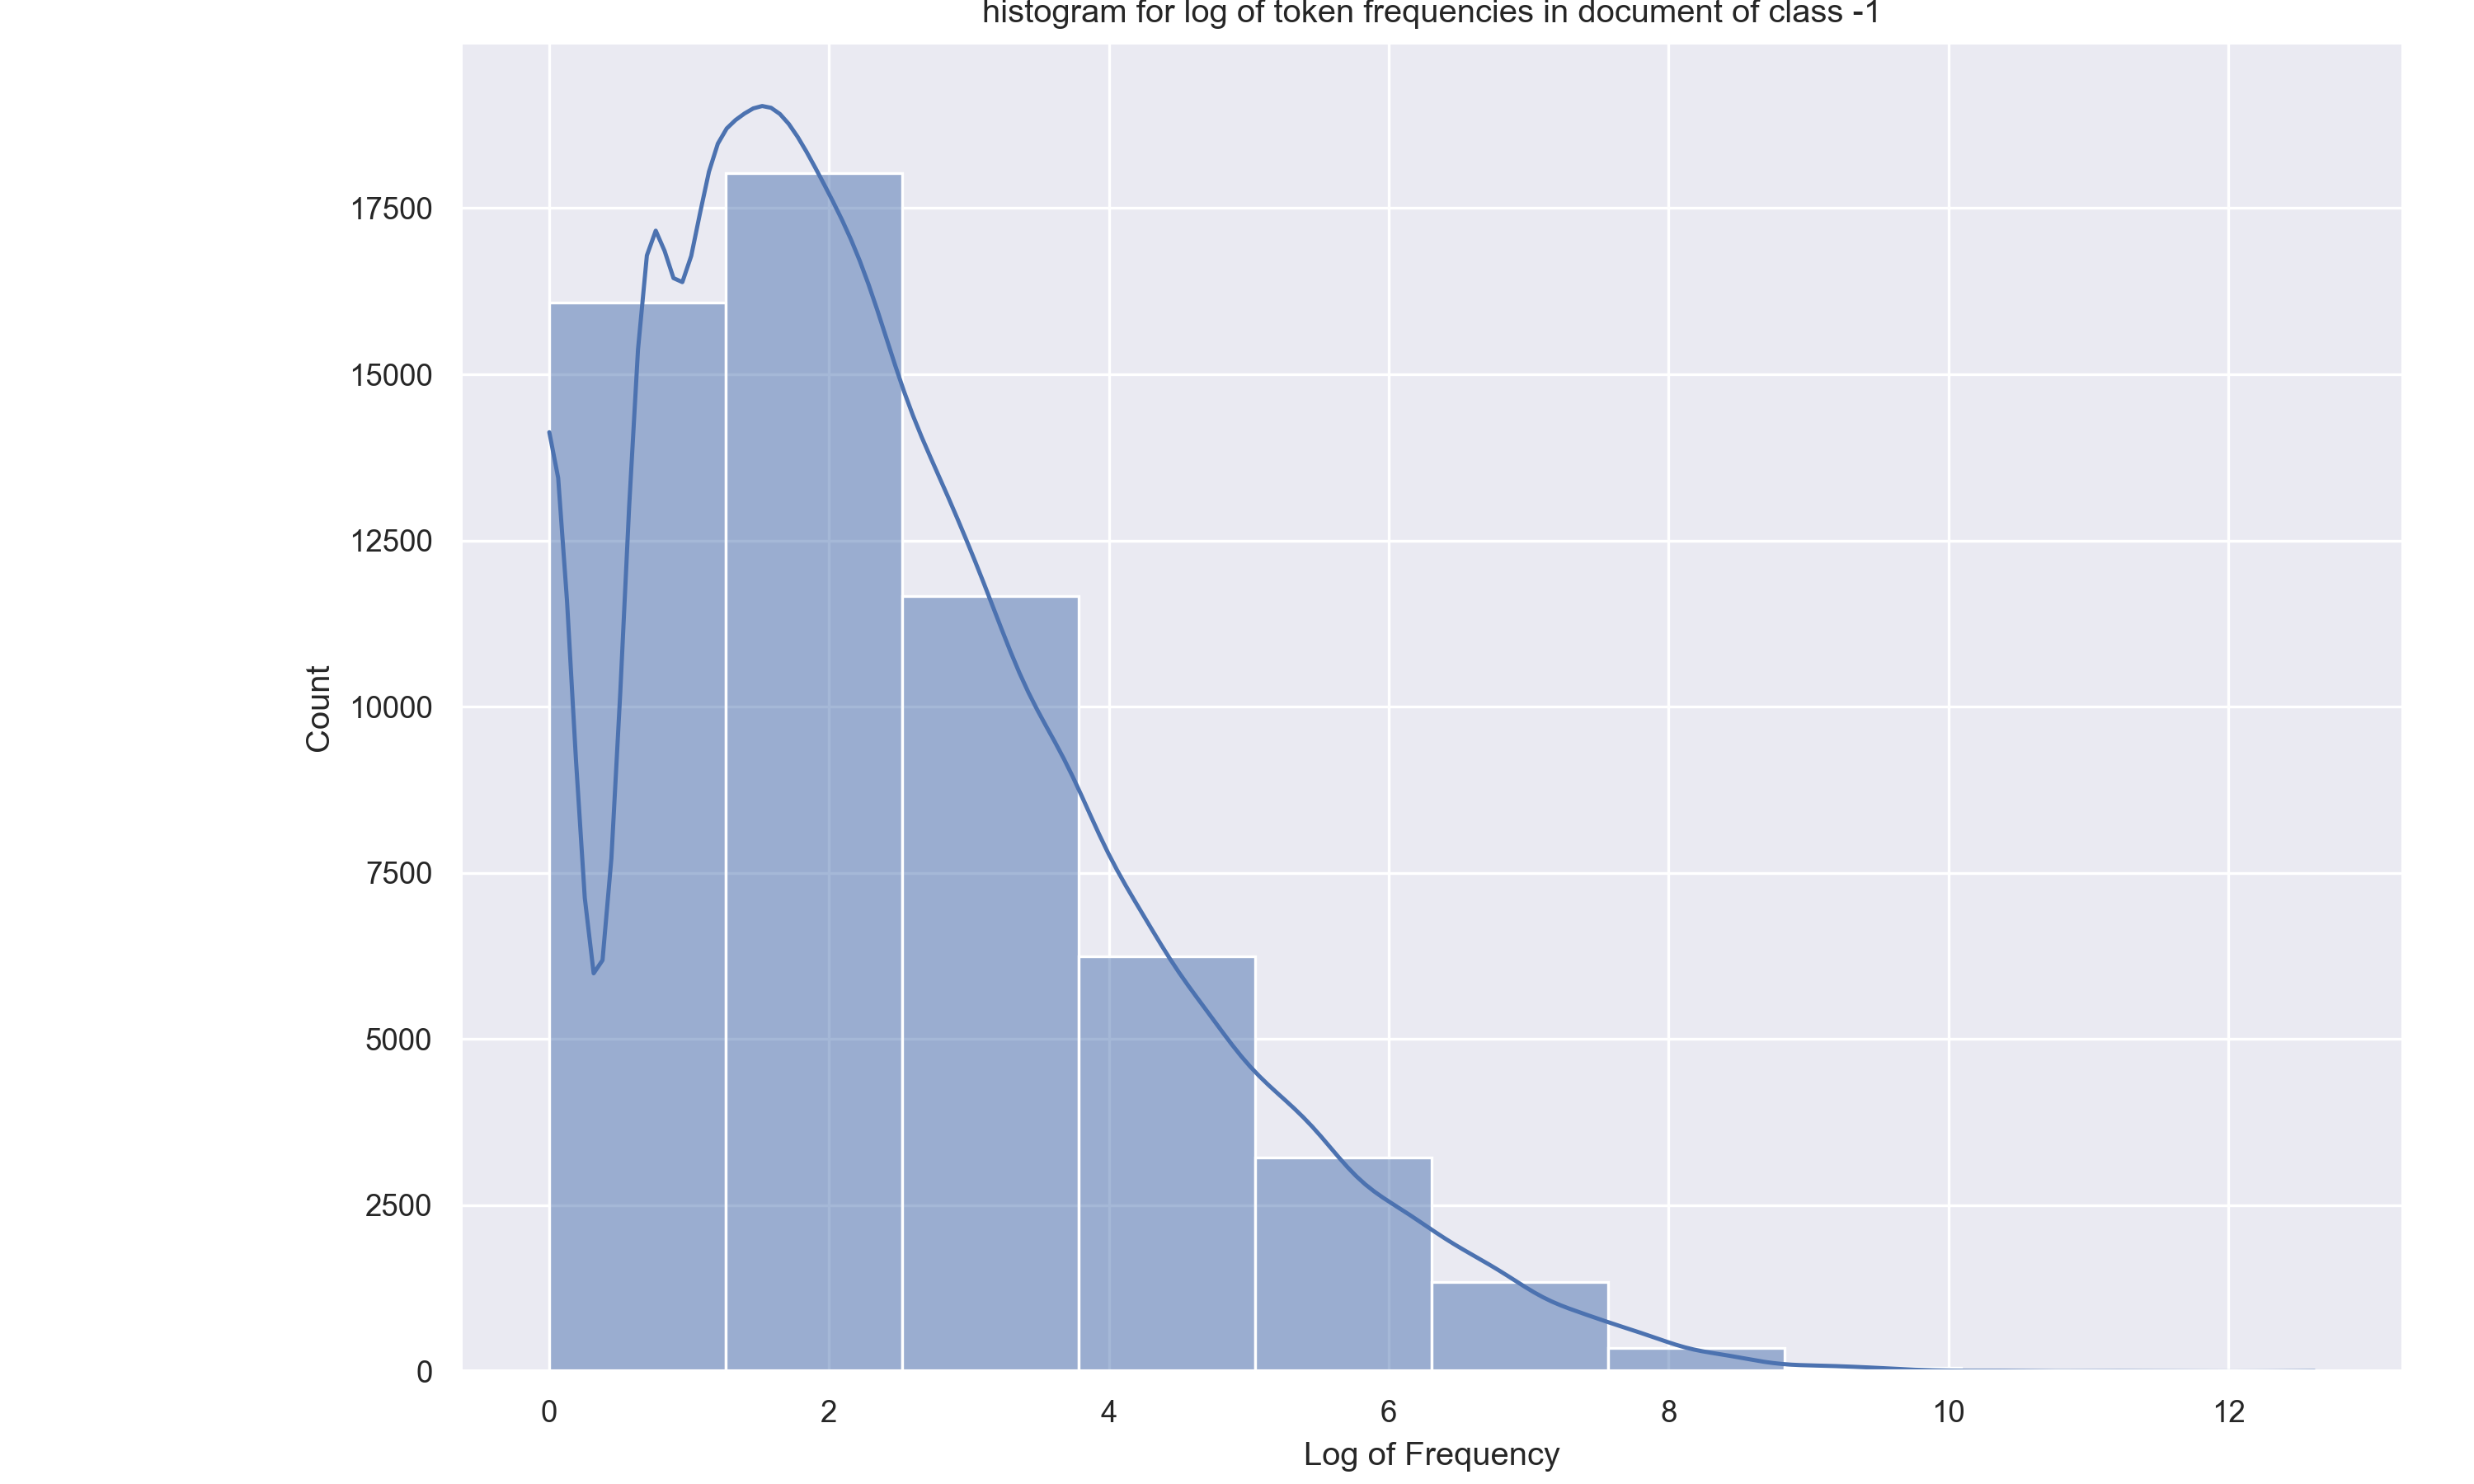
\includegraphics[width=0.65\textwidth]{figs/words_histogram/hist_token_-1.png}
\end{figure}
\end{center}

\pagebreak

\subsubsection{Bias Class 0 (Center)}
\begin{center}

\CatchFileDef{\TTTFIDFTable}{figs/words_histogram/table_0_token.latex.txt}

\TTTFIDFTable
\begin{figure}[h!]
  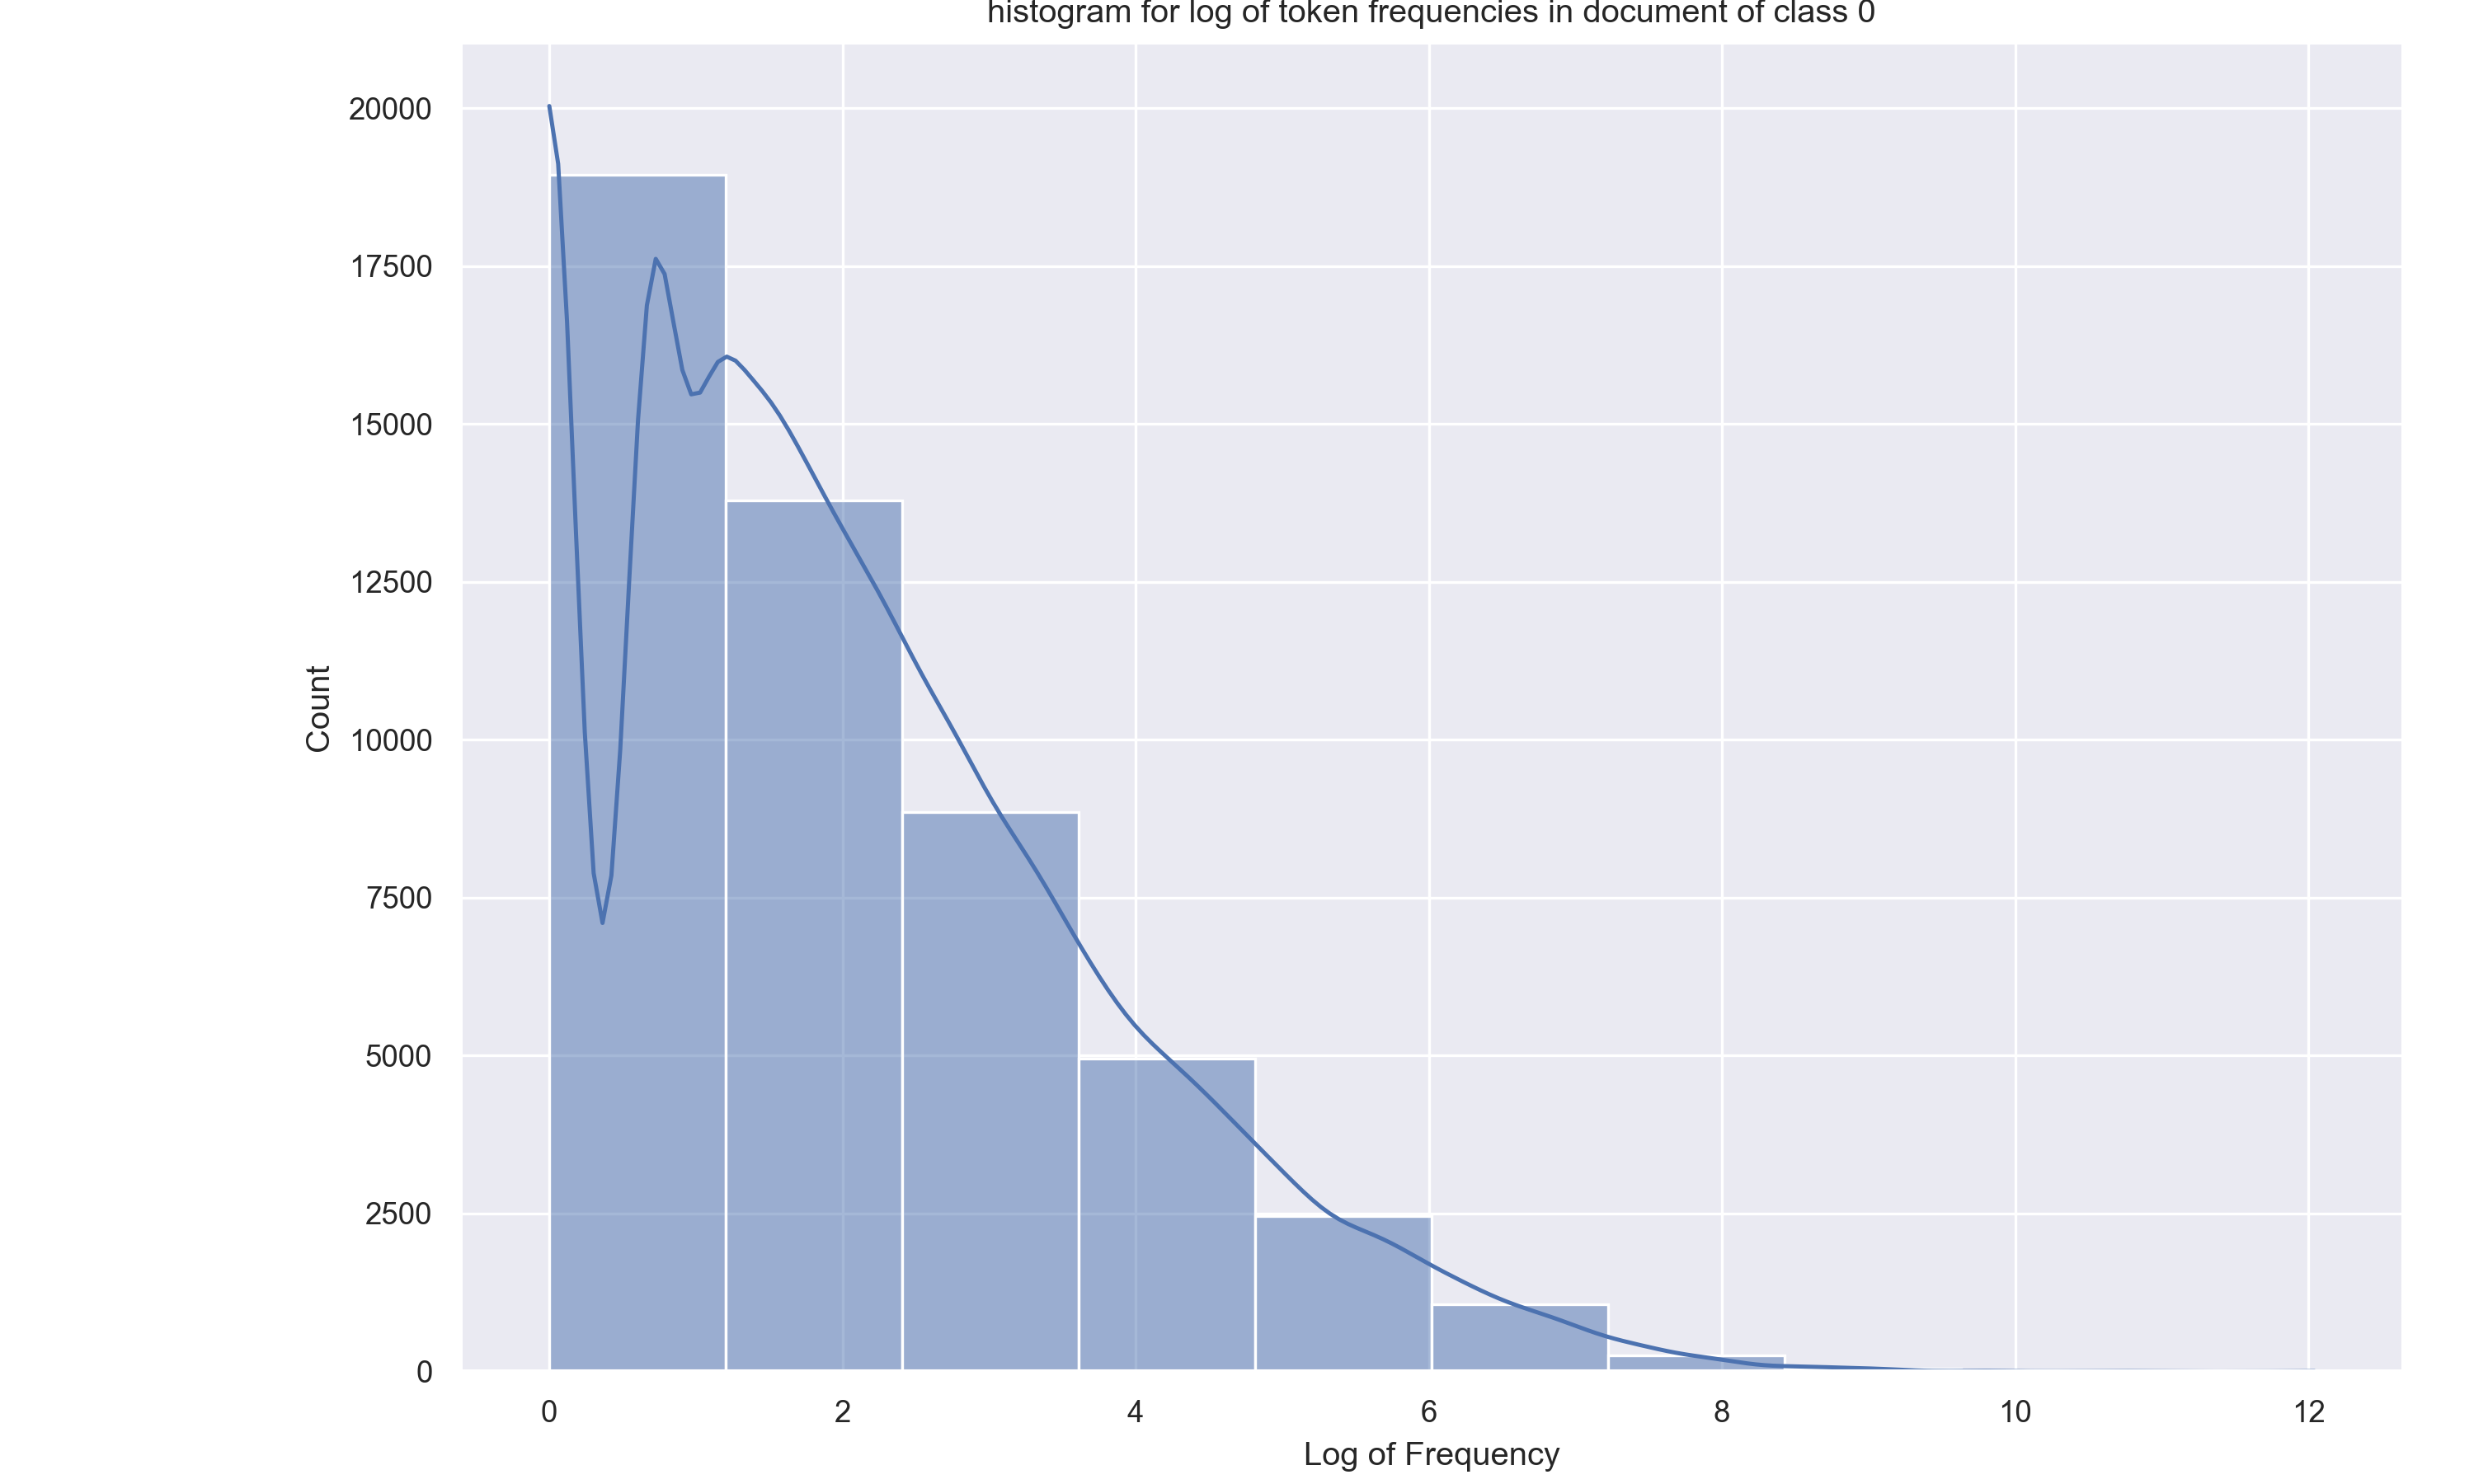
\includegraphics[width=0.65\textwidth]{figs/words_histogram/hist_token_0.png}
\end{figure}
\end{center}

\pagebreak

\subsubsection{Bias Class 1 (Center-Right)}
\begin{center}

\CatchFileDef{\TTTFIDFTable}{figs/words_histogram/table_1_token.latex.txt}

\TTTFIDFTable
\begin{figure}[h!]
  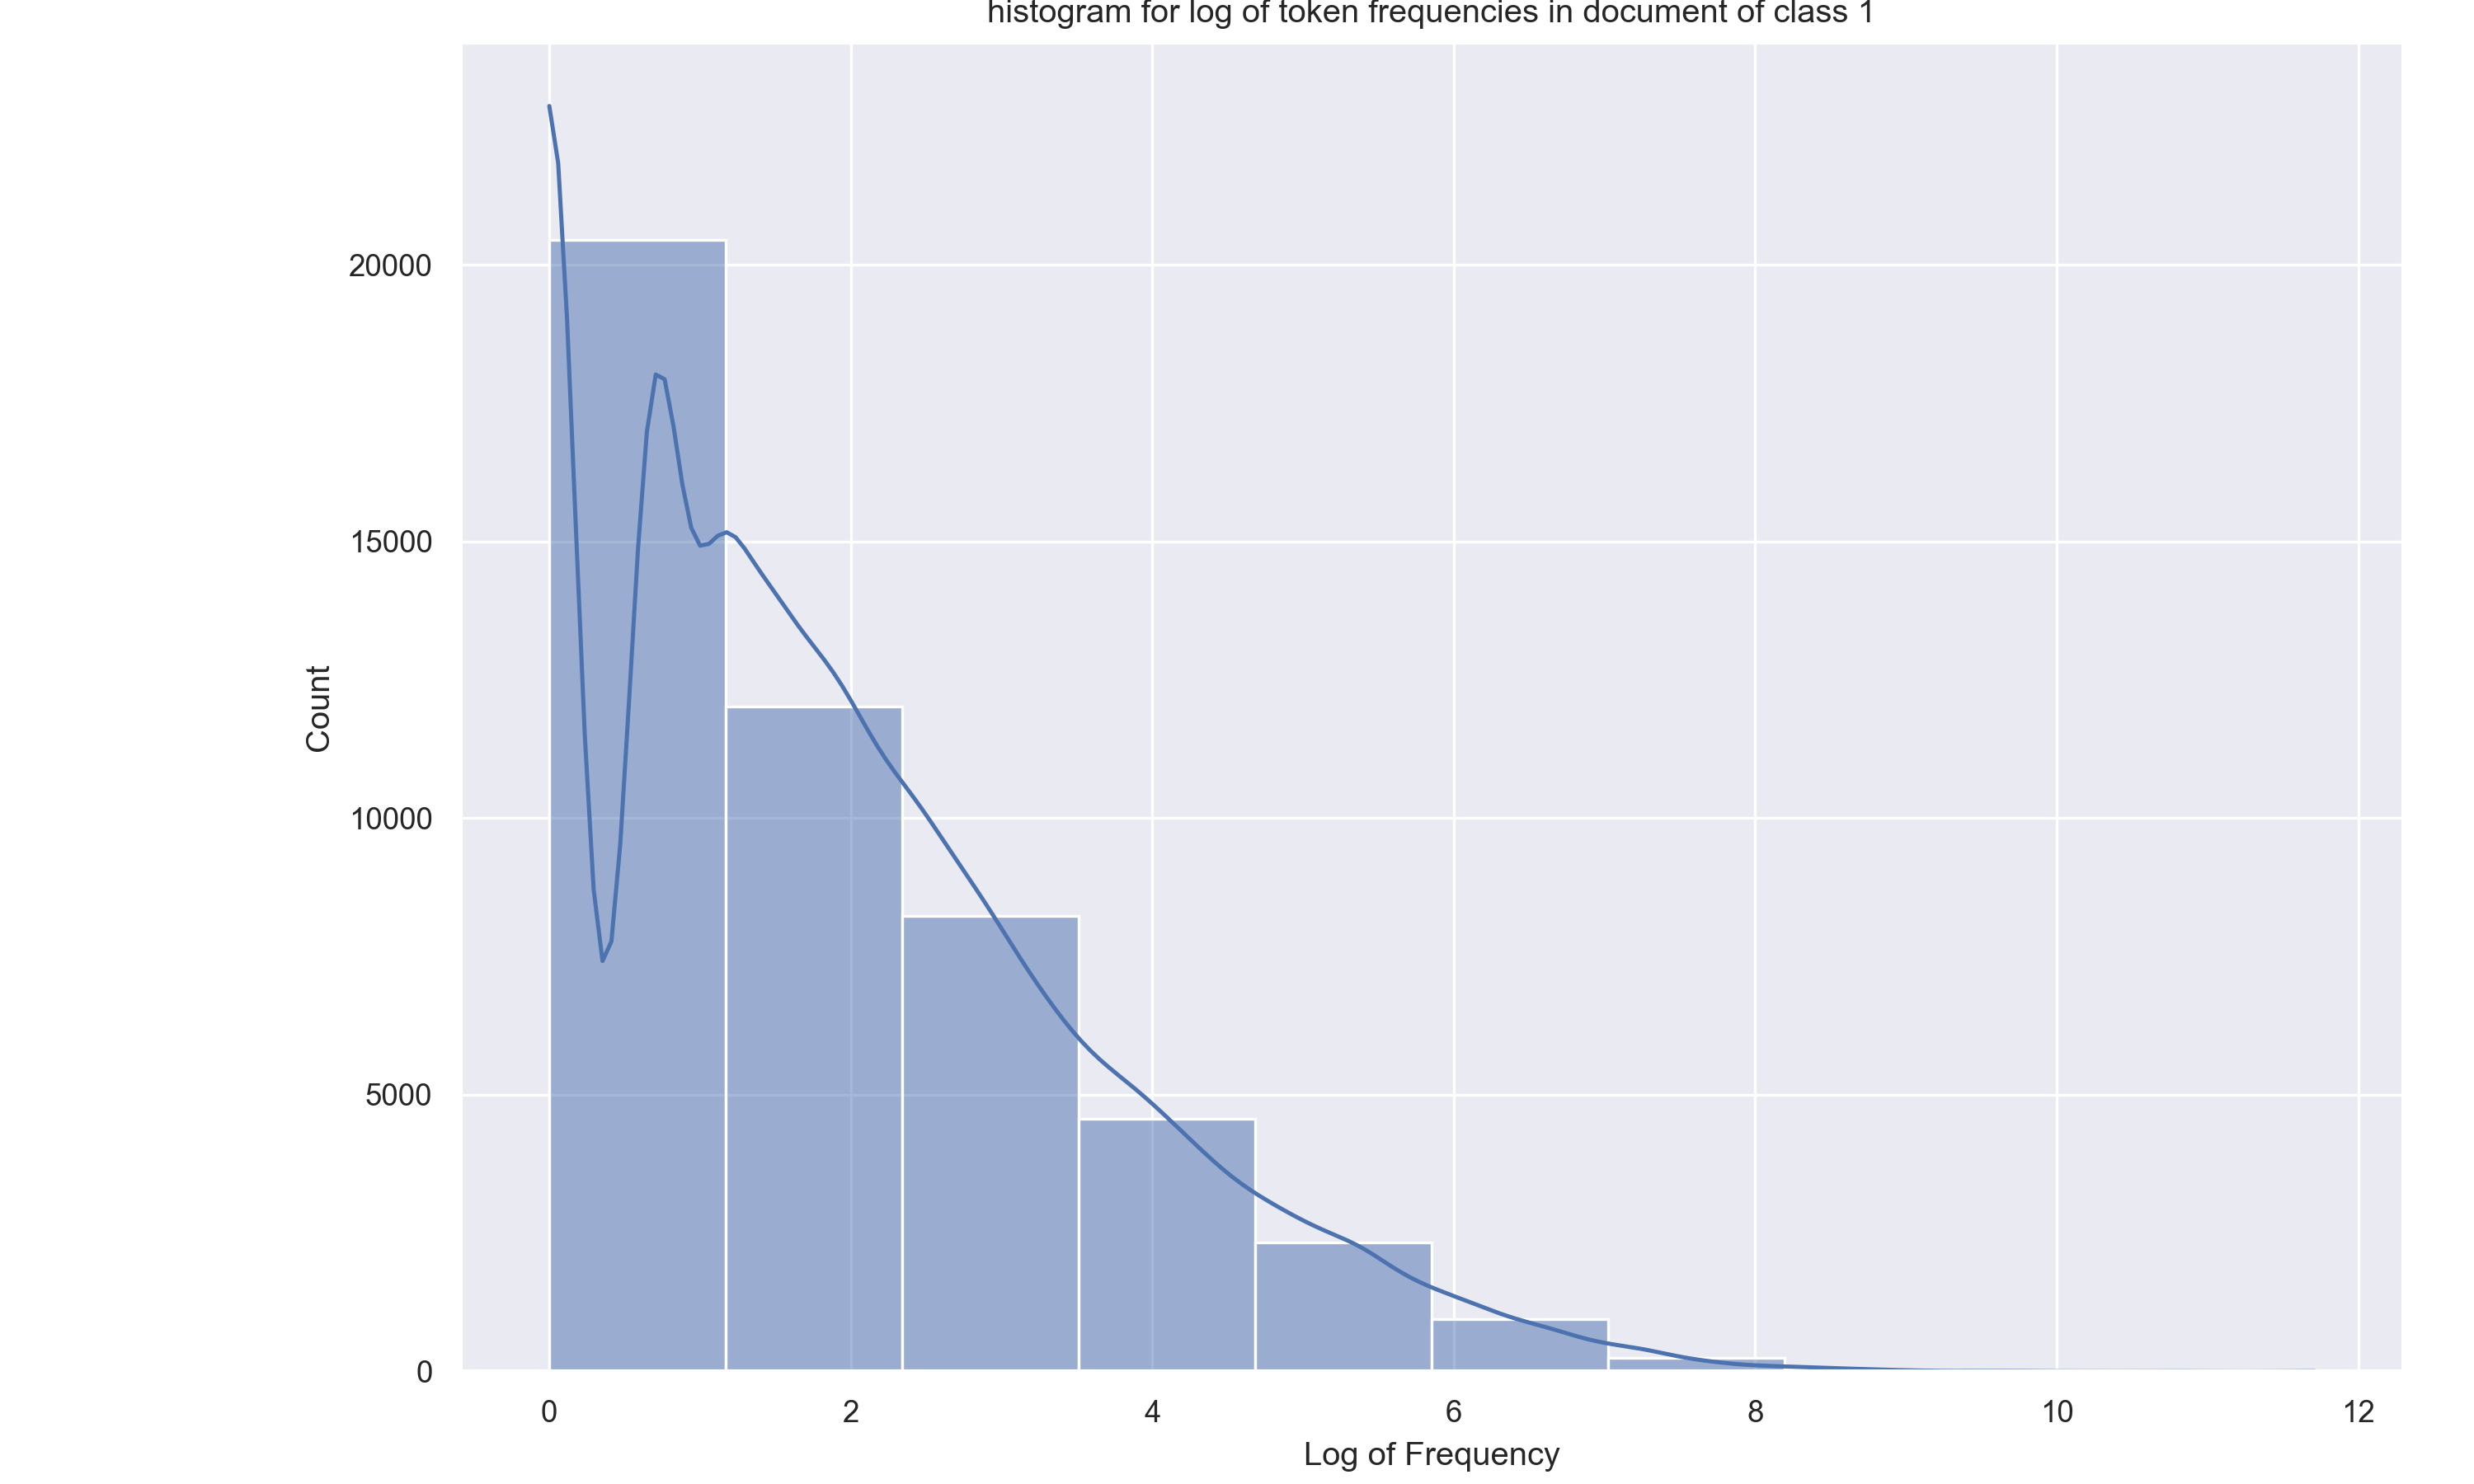
\includegraphics[width=0.65\textwidth]{figs/words_histogram/hist_token_1.png}
\end{figure}
\end{center}

\pagebreak

\subsubsection{Bias Class 2 (Right)}
\begin{center}

\CatchFileDef{\TTTFIDFTable}{figs/words_histogram/table_2_token.latex.txt}

\TTTFIDFTable
\begin{figure}[h!]
  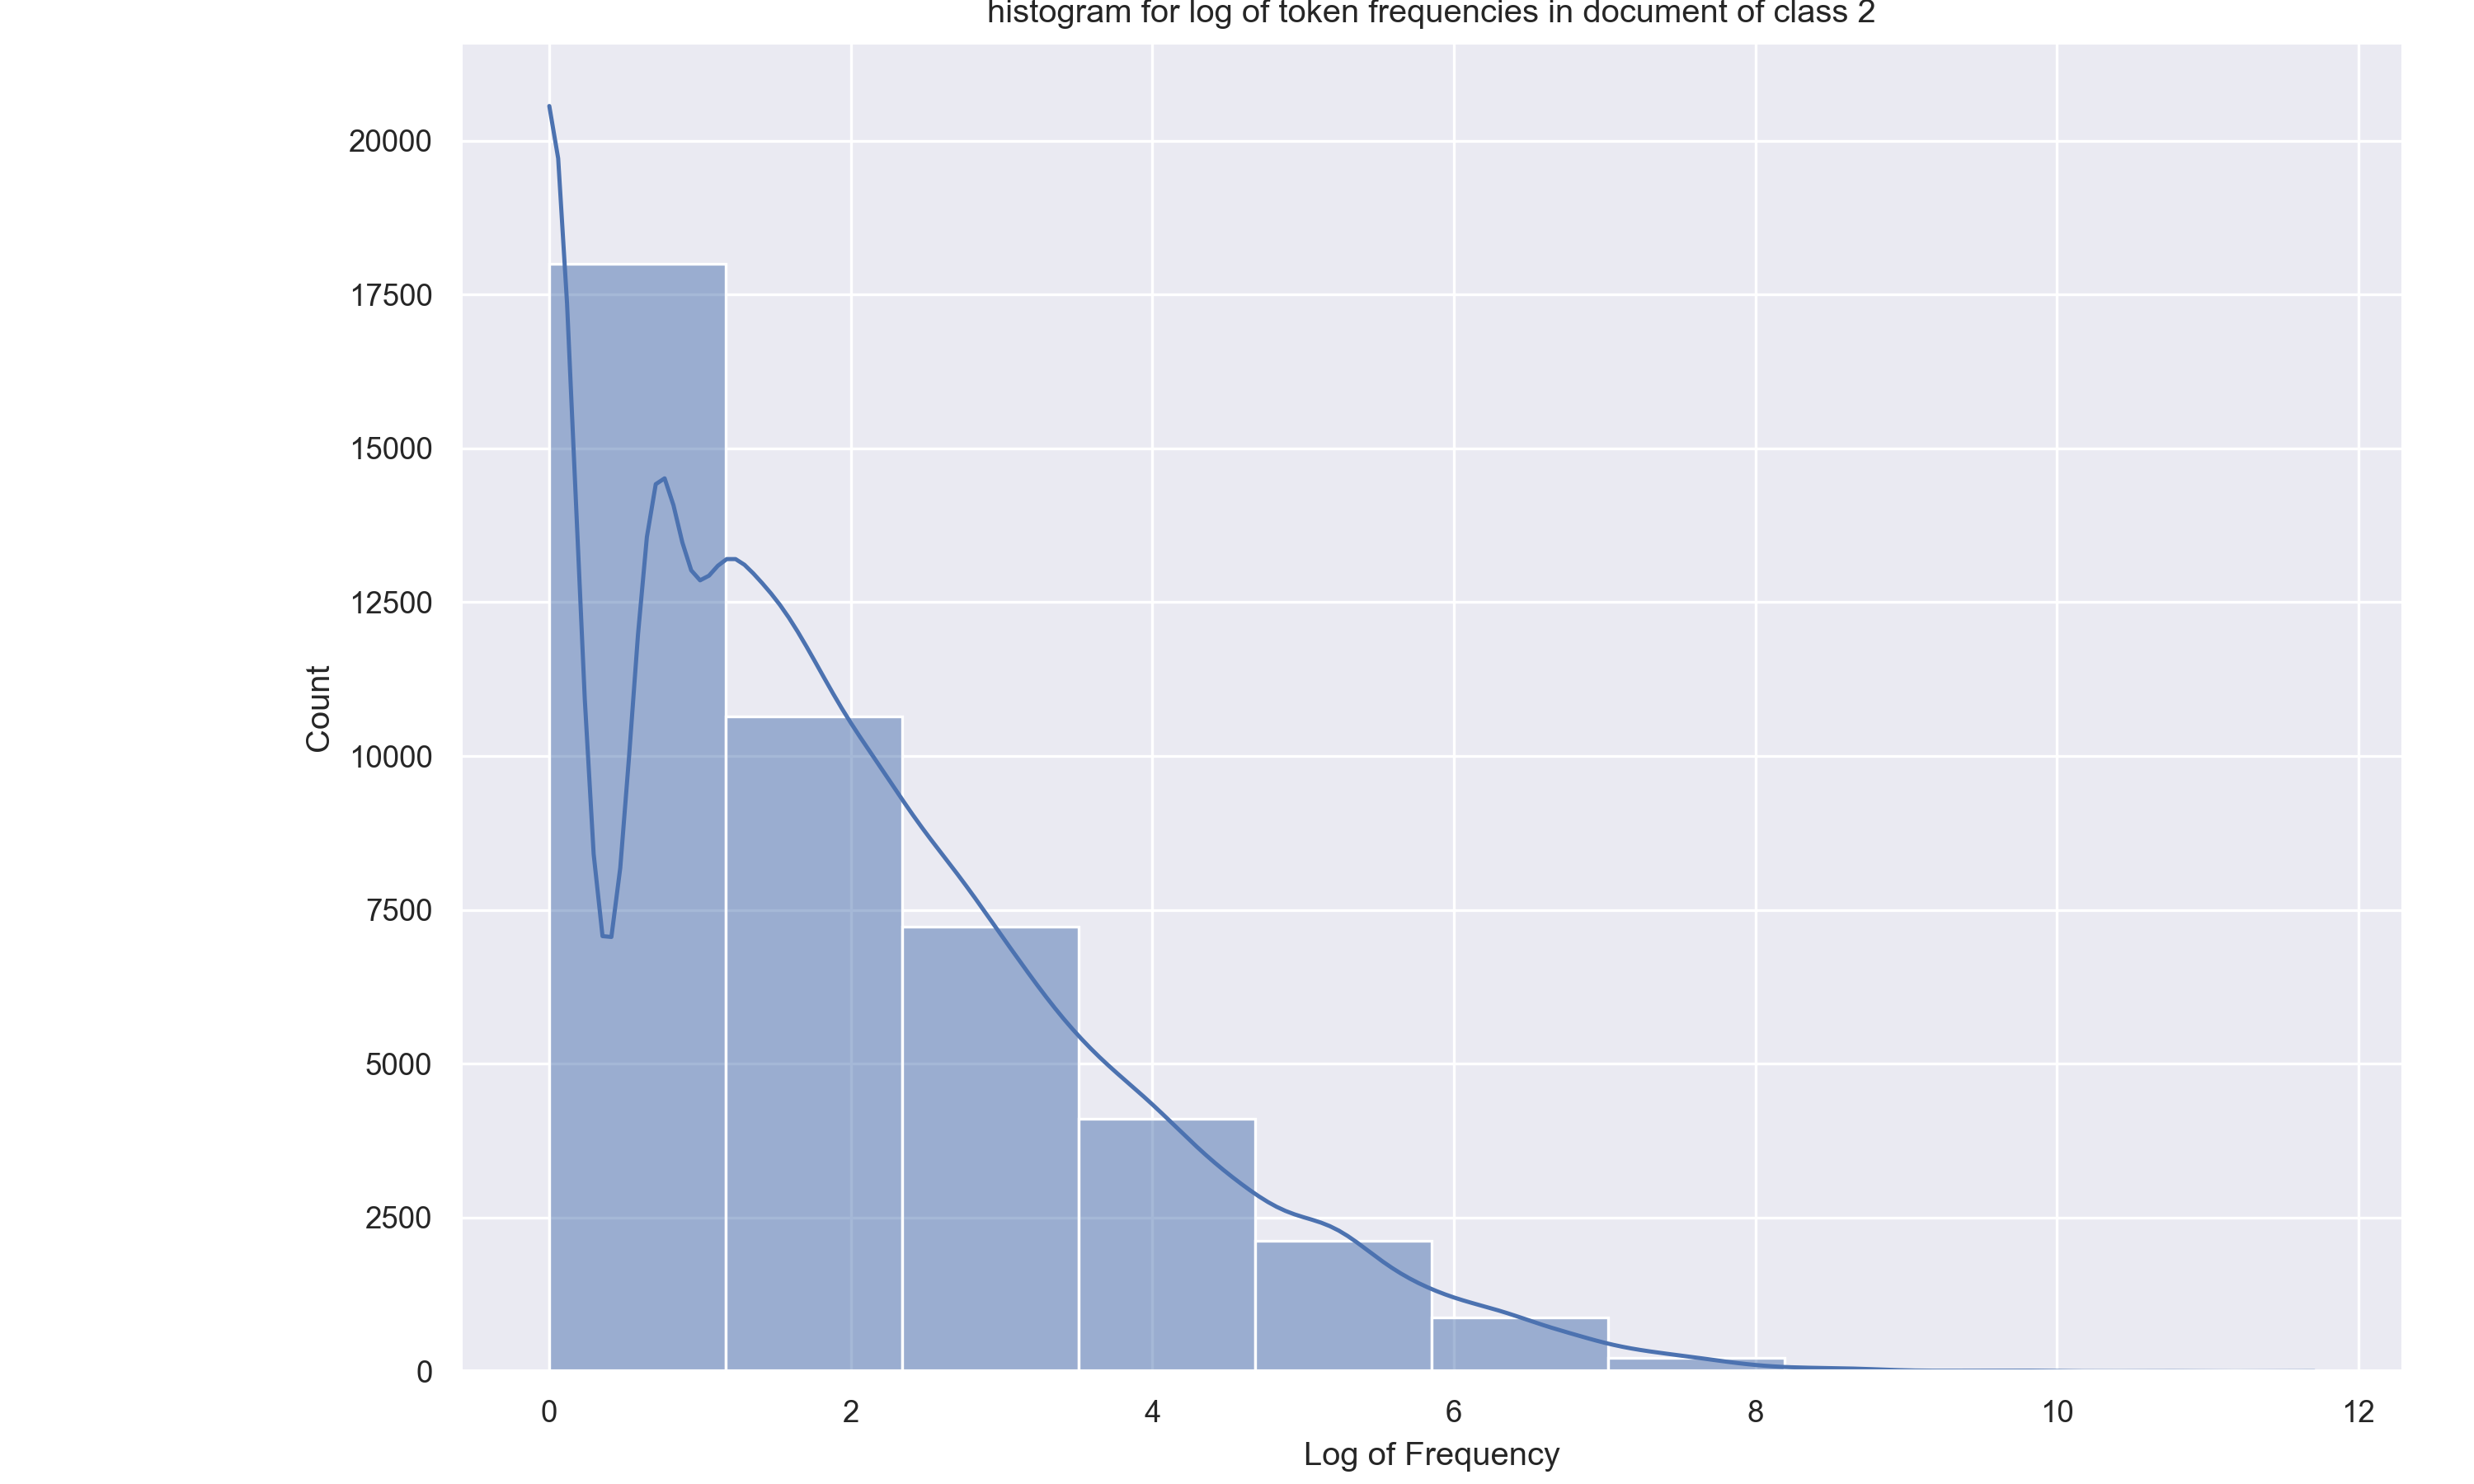
\includegraphics[width=0.65\textwidth]{figs/words_histogram/hist_token_2.png}
\end{figure}
\end{center}

\pagebreak

\subsection{Words Frequency Histogram}
\subsubsection{Bias Class -2 (Left)}
\begin{center}

\CatchFileDef{\TTTFIDFTable}{figs/words_histogram/table_-2_word.latex.txt}

\TTTFIDFTable
\begin{figure}[h!]
  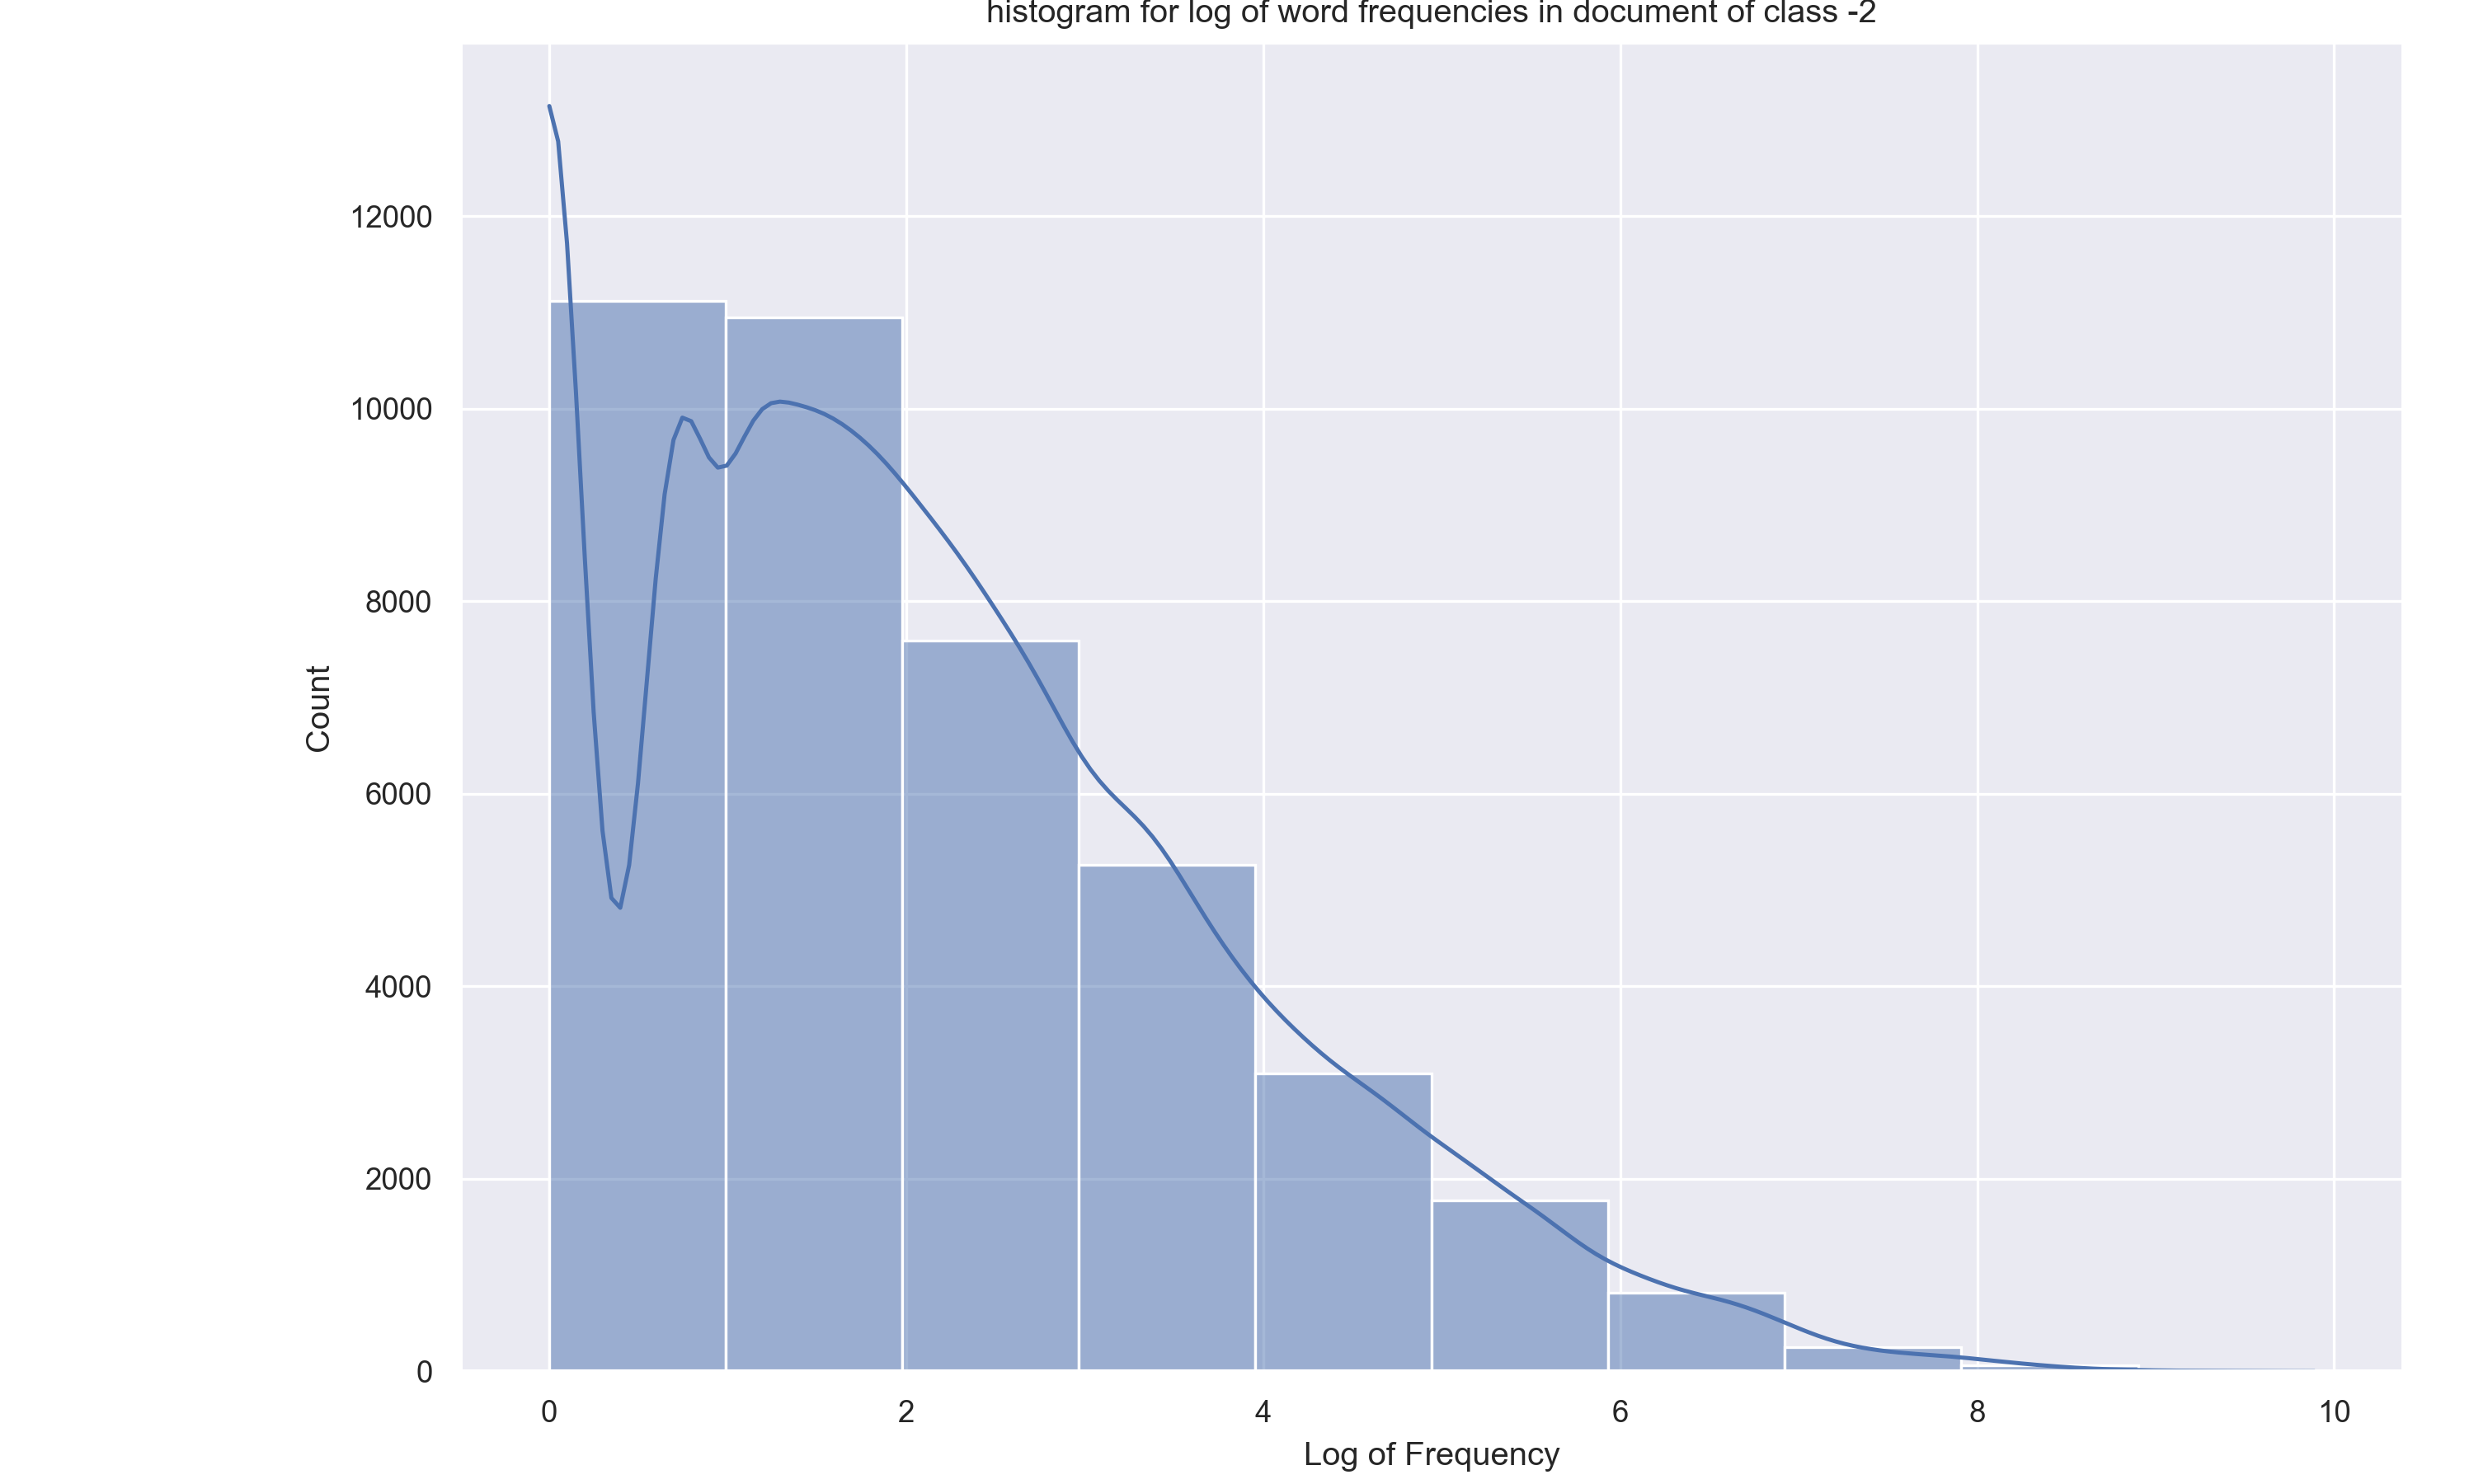
\includegraphics[width=0.65\textwidth]{figs/words_histogram/hist_word_-2.png}
\end{figure}
\end{center}

\pagebreak

\subsubsection{Bias Class -1 (Center-Left)}
\begin{center}

\CatchFileDef{\TTTFIDFTable}{figs/words_histogram/table_-1_word.latex.txt}

\TTTFIDFTable
\begin{figure}[h!]
  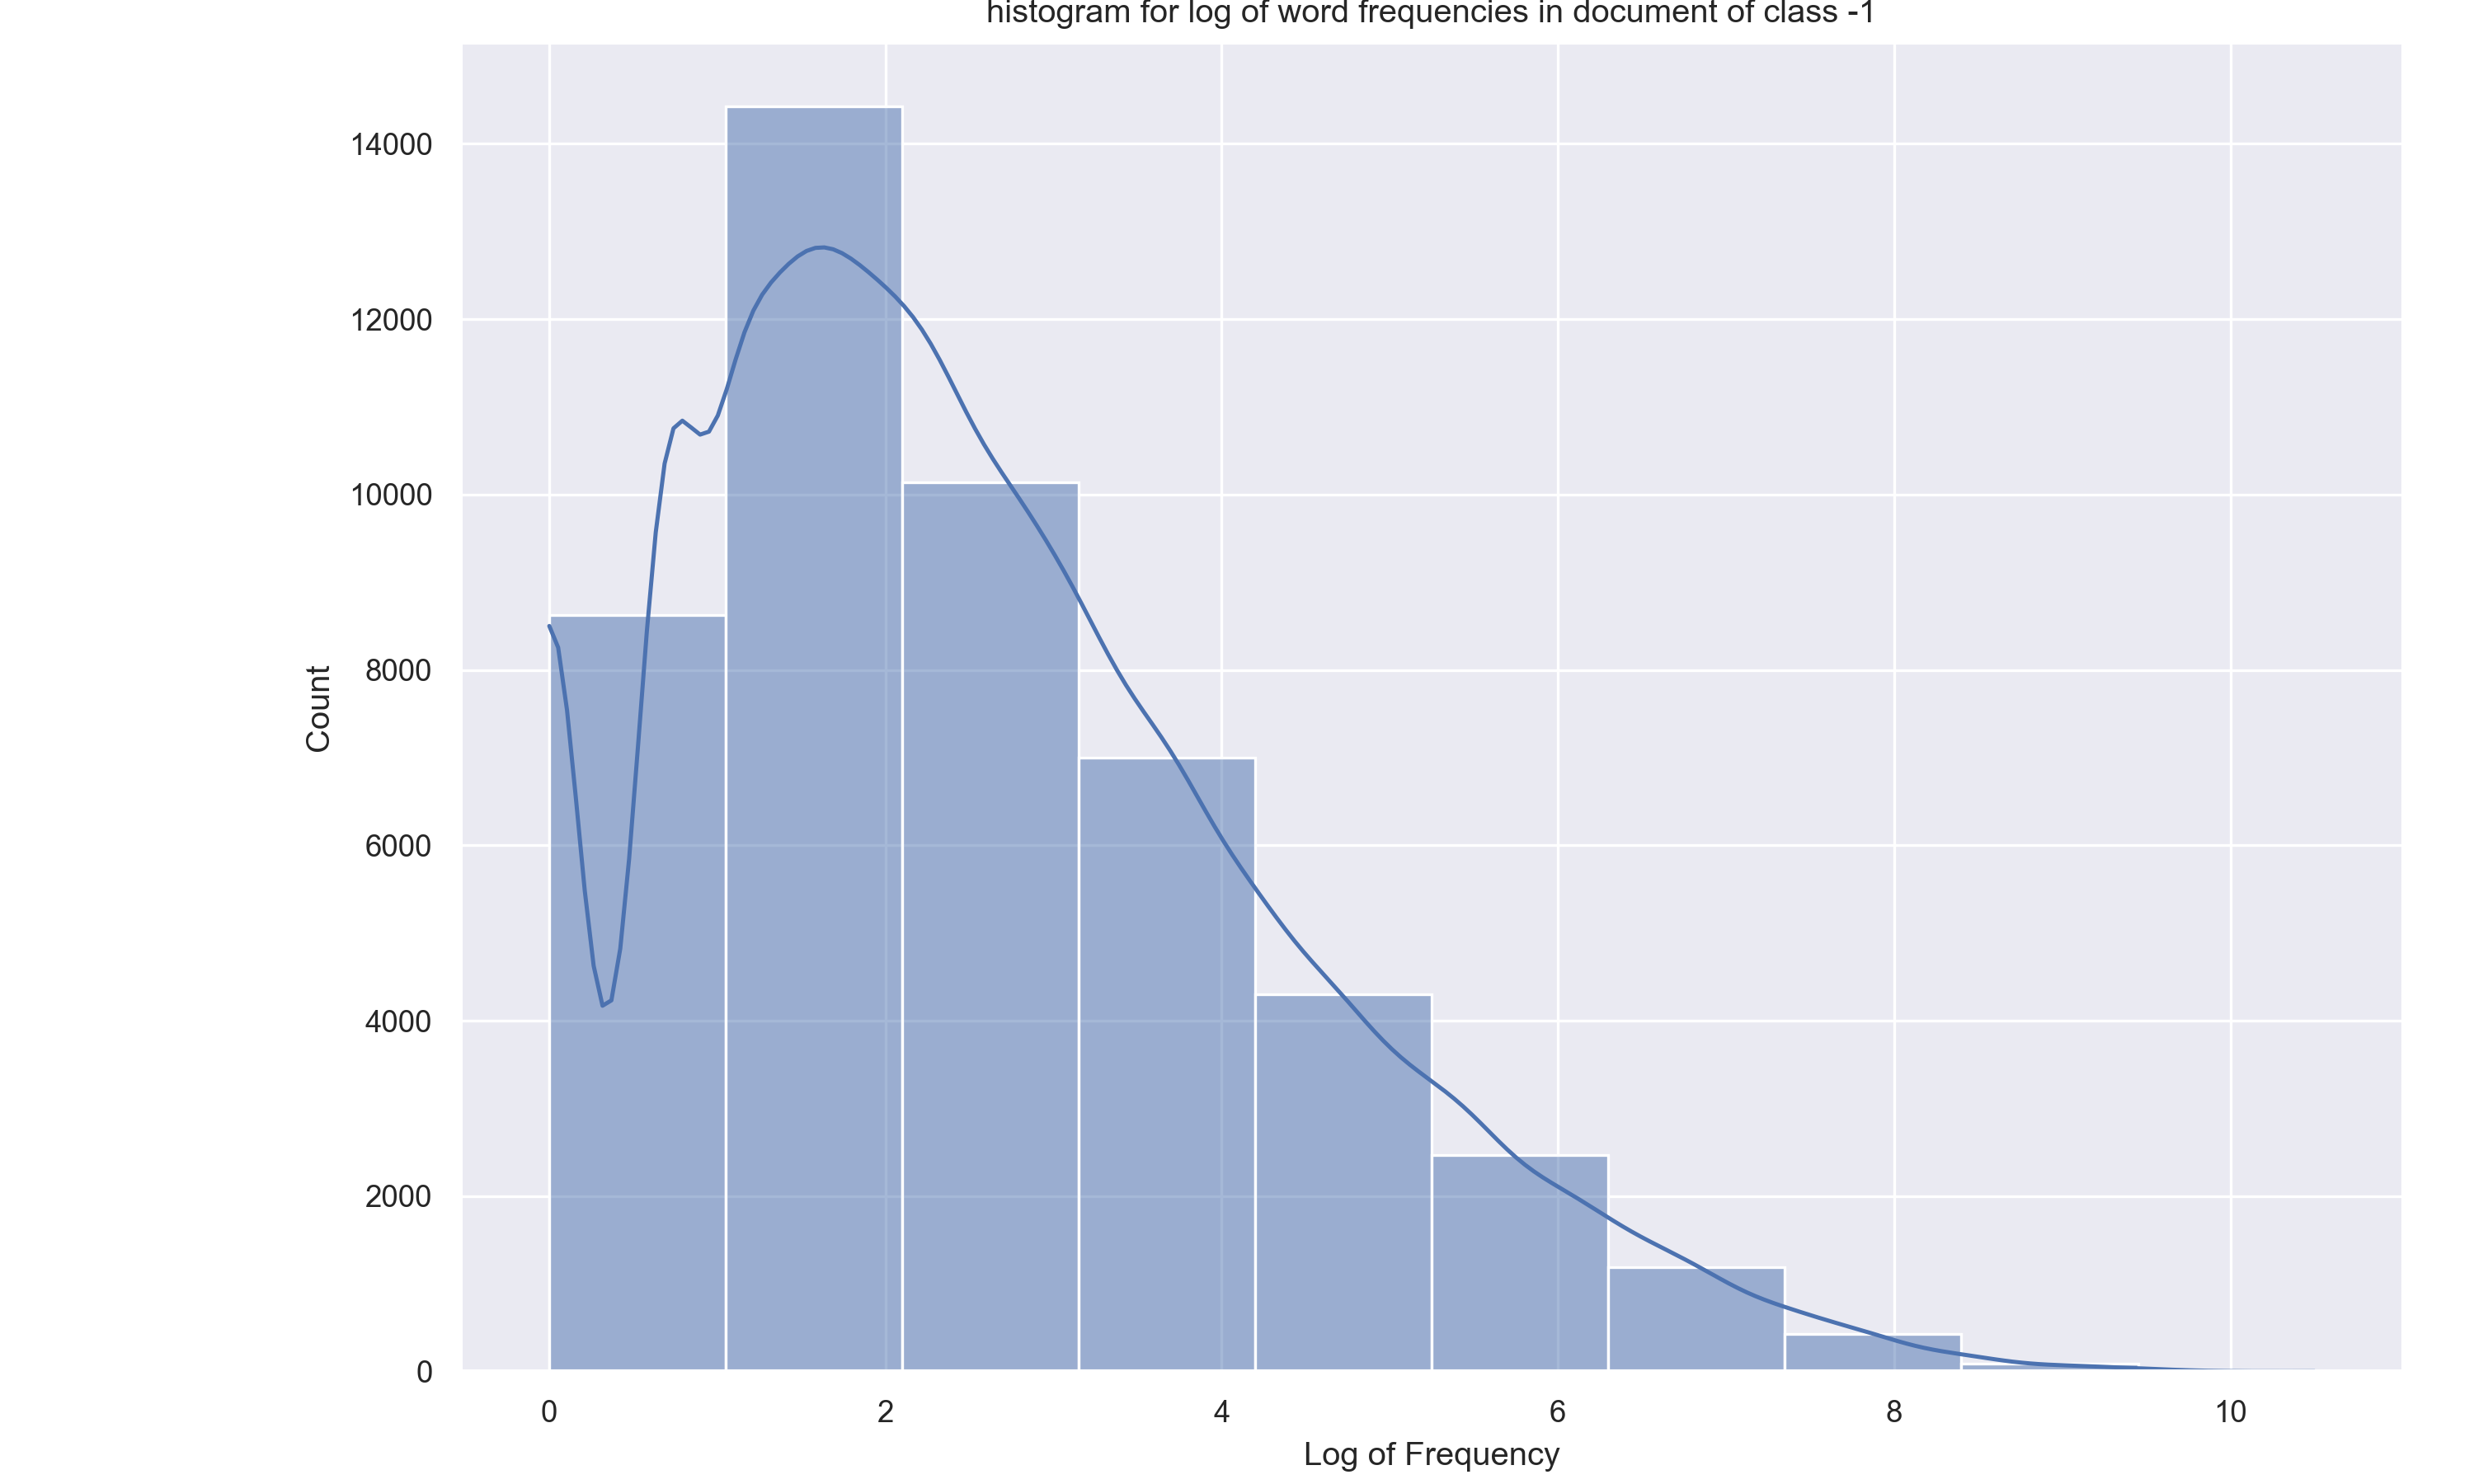
\includegraphics[width=0.65\textwidth]{figs/words_histogram/hist_word_-1.png}
\end{figure}
\end{center}

\pagebreak

\subsubsection{Bias Class 0 (Center)}
\begin{center}

\CatchFileDef{\TTTFIDFTable}{figs/words_histogram/table_0_word.latex.txt}

\TTTFIDFTable
\begin{figure}[h!]
  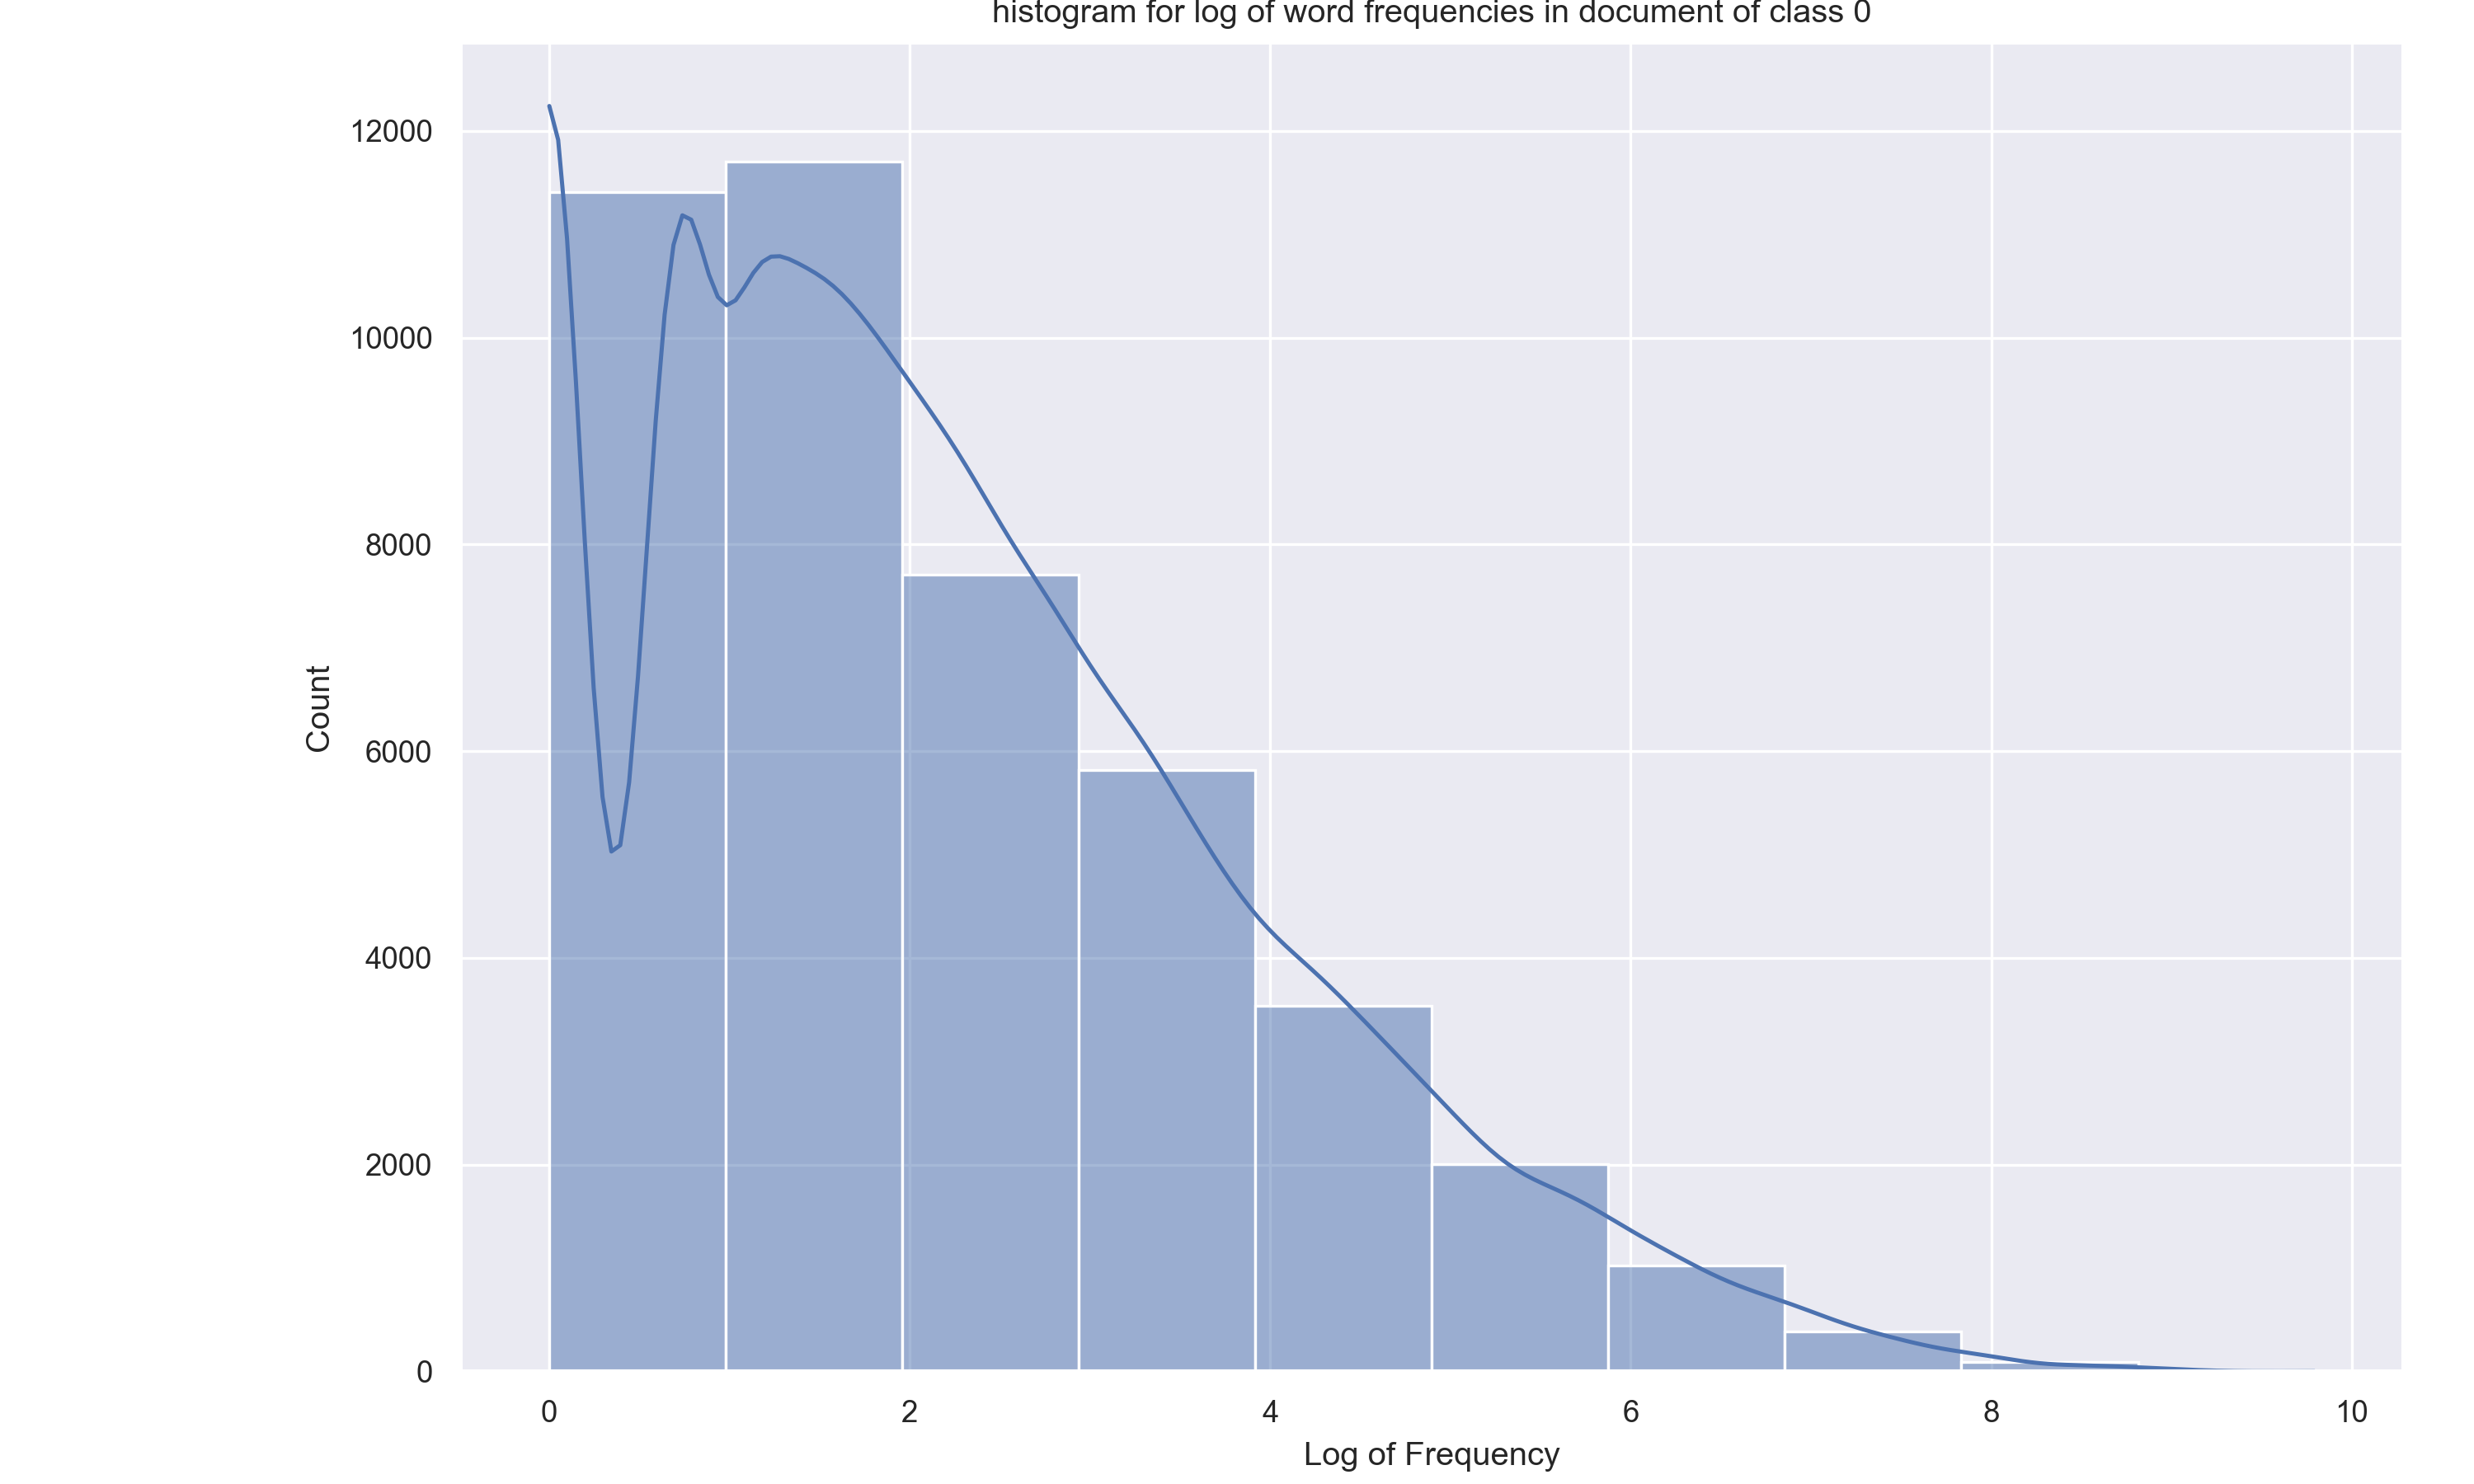
\includegraphics[width=0.65\textwidth]{figs/words_histogram/hist_word_0.png}
\end{figure}
\end{center}

\pagebreak

\subsubsection{Bias Class 1 (Center-Right)}
\begin{center}

\CatchFileDef{\TTTFIDFTable}{figs/words_histogram/table_1_word.latex.txt}

\TTTFIDFTable
\begin{figure}[h!]
  \includegraphics[width=0.65\textwidth]{figs/words_histogram/hist_word_1.png}
\end{figure}
\end{center}

\pagebreak

\subsubsection{Bias Class 2 (Right)}
\begin{center}

\CatchFileDef{\TTTFIDFTable}{figs/words_histogram/table_2_word.latex.txt}

\TTTFIDFTable
\begin{figure}[h!]
  \includegraphics[width=0.85\textwidth]{figs/words_histogram/hist_word_2.png}
\end{figure}
\end{center}

\end{document}